\documentclass{article}
\usepackage[utf8]{inputenc}
\usepackage[dvipsnames]{xcolor}
\usepackage{graphicx}        % standard LaTeX graphics toolhttps://www.overleaf.com/project/5e6ada755bf39e0001fe46c0
\usepackage{float} 
\usepackage{mathtools}
\usepackage{hyperref}
\usepackage{wasysym}
\usepackage{adjustbox}
\usepackage{nicefrac}
\usepackage{xfrac}    % for \sfrac
\usepackage{verbatim} 
\usepackage{xcolor}
\usepackage[style=apa]{biblatex}
\addbibresource{references.bib}

\newcommand{\rocco}[1]{{\textcolor{red}{Rocco: #1}}} % to add comments
\newcommand{\andreas}[1]{\textcolor{blue}{{Andreas: }#1}} % to add comments


\title{Relocation choice for different homophily preferences: hybrid scenarios for Schelling Model\\
\ title to define
}

\author{Rocco Paolillo, Andreas Flache}
\date{March 2021}

\begin{document}

\maketitle

\begin{abstract}
[shorten to 200 wrds]   Schelling’s model of residential segregation famously showed how high levels of residential segregation can emerge as unintended outcome of the interplay of individual relocations of actors who hold relatively mild ethnic preferences. Most of the work building on this model neglected two forms of heterogeneity which seem to become increasingly important empirically in contemporary societies. First, there is considerable heterogeneity of residential preferences not only between but also within ethnic groups, with especially younger, higher educated and more wealthy individuals having less strong preferences for ethnic homophily. Second, most of the research following Schelling focuses on ethnic similarity as relevant to residential preferences. However, recent theoretical and empirical research on spatial sorting emphasizes multidimensionality, as individuals prefer similar others not only regarding ethnicity, but also for social distinctions as shared values or shared status. Extending recent work (Paolillo et Lorenz, 2018), we explore the interplay of heterogeneity in both forms of homophily preferences for ethnicity and shared values. Using a discrete choice version of Schelling’s model, in which agents differ in their relative weights for ethnic and value similarity in relocation moves, we explore the consequences of deterministic or random relocation choice of agents, in addition to structural conditions of relative group sizes of ethnic and value groups. We find in particular that hybrid segregation patterns can emerge in which ethnically mixed but value homogeneous neighborhoods arise alongside ethnically segregated neighborhoods populated by agents driven more by ethnic homophily. Importantly and contrary to Schelling’s model, we show how partial ethnic mixing can arise even if everyone has a preference for more co-ethnics in her neighborhood, all other things being equal.
\end{abstract}

\keywords{Keywords (3-5): super-diversity, discrete choice, spatial sorting, Schelling}


\section*{Introduction}

% Topic: from General Segregation, to the specific how Schelling gets in

Ethnic or racial residential segregation appears still a critical topic of multi-ethnic cities all over the world \autocite{charles2003dynamics}. Many possible and interconnected explanations for segregation have been proposed, such as discrimination by landlords \autocite{ahmed2008discrimination}, the sorting mechanisms built into housing markets \autocite{bailey2012spatial}, or income inequality in combination with features of urban geography \autocite{pais2017intergenerational}. Prominently, Schelling's contribution was to demonstrate   \autocite{schelling1969models,schelling1971dynamic} with a formal computational model that segregation can be a self-organizing phenomenon (unorganized segregation) that emerges from the interaction of people satisfying their "discriminatory individual choice" \textcite[p. 488]{schelling1969models} within spatial limited constraints\footnote{Essentially the same mechanism proposed by Schelling was independently developed and formalized earlier by \textcite{sakoda1971checkerboard}, see \textcite{hegselmann2017thomas}}. Essential to Schelling's model, and focus of this paper, is the concept of "preference dynamics" \autocite{clark2008understanding}, i.e. the empirically plausible assumption that people typically want at least a certain minimal fraction of co-ethnics nearby, even if they are content with living in a mixed neighborhood. One key insight from a large number of formal modelling studies is the robustness of the main results of the model \autocite{flache2020analytical}, also if people hold "integrationist" preferences \autocite{zhang2004} or randomness is included in residential choices of agents \autocite{bruch2006neighborhood,van2009neighborhood,bruch2009preferences}. The robustness of segregation due to preferences persists also when they are combined with additional parameters as housing pricing and income differences \autocite{fossett2006ethnic}, relative group sizes \autocite{bruch2014population} or empirically realistic spatial structures of real cities \autocite{benenson2009schelling}.

Yet, despite the strong theoretical and empirical evidence that preference dynamics might suffice to generate robust and high levels of ethnic segregation, recent trends in residential segregation suggest a somewhat different and more complex picture from the premises of Schelling's original model. 
As regards ethnic segregation, not only do U.S. studies point to declining levels in recent decades (e.g. \textcite{glaeser2012end}) compared to the 60’s/70’s urban landscape \autocite{clark2015residential} Schelling referred to \autocite{schelling1969models}, but also mixed neighborhoods increasingly start to arise in multi-ethnic cities \autocite{clark2015residential, lee2012racial}. This pattern is also reflected in studies from Europe \autocite{blokland2010people}. In addition to deeply variegated society \autocite{lee2012racial}, it has been suggested that this pattern can be attributed to changes in residential preferences. Goldman (2012), for example, finds evidence of reduced racial prejudice in the society as a whole, a trend that seems to extend to residential ethnic preferences \autocite{xie2012modeling}. Furthermore, residential preferences can vary according to socio-demographic characteristics. On the whole, it appears that younger \autocite{clark2018can, clark2009changing}, more highly educated and higher income citizens have increasingly more tolerant ethnic preferences \autocite{clark2019neighborhood,crowder2012neighborhood,clark2009changing,xie2012modeling} when it comes to residential choice. A common trait of modern societies is that these socio-demographic characteristics and the social preference associated are differently distributed both within \autocite{clark2002residential,crul2017upcoming} and between ethnic groups \autocite{clark2009changing,crowder2012neighborhood}. Thus, differently from Schelling, it becomes a both theoretically and empirically plausible scenario that members of the same ethnic group experience different degree of integration or segregation along diverse dimensions in addition to ethnicity. In this paper, we are interested in this aspect we refer to as "hybrid segregation" and we aim at modeling possible scenarios of how it can come to be.

Formal models of Schelling-type preferences dynamics have recently started to incorporate the insight that individuals differ in the degree of tolerance to local ethnic diversity. These models imposed heterogeneity in the desired neighborhood proportion of co-ethnics \autocite{xie2012modeling, hatna2014combining}. Interestingly, these studies found that - similar to empirical patterns observed in modern multi-ethnic cities - preference dynamics could give rise to a division between ethnically mixed and segregated neighborhoods co-existing in the same city, together with a selection of more tolerant agents into the mixed neighborhoods. However, there is another important form of preference heterogeneity these models have not taken into account and which could profoundly affect dynamics of segregation. Shared values, defined as common beliefs, preferences or expectations on acceptable behavior induce perceptions of similarity across the boundaries of ethnicity \autocite{wimmer2013ethnic,bail2008configuration}. In modern societies where individuals differ along many and different social distinctions \autocite{vertovec2007super}, shared values can become even more important than ethnicity itself. Recent empirical studies, indeed, suggest that a preference for value-similar neighbors may sometimes even dominate preferences for ethnic similarity. For instance,\textcite{van2019sociocultural} show how similarity with neighbors in sociocultural dispositions (i.e. gender balance in household tenure) is a better predictor to leave the neighborhood, compared to ethnic membership and income similarity. In a similar vein, research on homophily in social networks recently has moved forward to recognize the importance of multidimensional similarity for the formation of social relationships \autocite{block2014multidimensional,hooijsma2020multidimensional}. This research shows that dissimilarity in ethnicity might not negatively affect the formation of relationships when compensated for by salient similarities individuals perceive in other categories. 


While recent empirical studies seem to adopt the interplay of ethnicity with other social distinctions to explain hybrid segregation in diverse societies, this seems rarely the case in modeling literature. Yet, we argue that this work points to an intriguing new possibility for residential segregation dynamics and hybrid segregation scenarios. The seemingly unstoppable march towards segregation that Schelling-type preference dynamics induce may not only be stopped by higher levels of ethnic tolerance, as suggested by \textcite{xie2012modeling} or \textcite{hatna2014combining}. It may also be stopped in a world where individuals still prefer being among co-ethnics, but at the same time hold an even stronger preference for having neighbors with similar values who also happen to be members of other ethnic groups. Given that such a predominance of value-orientation in residential preferences appears to some extent to be correlated with education, income or age, this possibility would offer a new explanation in the framework of Schelling-type preference dynamics of why well-off younger generations appear to increasingly move to more affluent and more ethnically mixed neighborhoods \autocite{clark2018can,clark2002residential}. It would also help to understand why low-income strata seem to become increasingly segregated through generations, meaning that their neighborhoods become progressively both ethnically and economically segregated \autocite{clark2002residential}. 
%%%%

% An antecedent Paolillo & Lorenz who had the intuition of value preferences. Why a good venue: showed a hybrid scenario, establish multidimensional homophily preferences

In this paper, we propose a formal computational model of Schelling-type preference dynamics that incorporates the interplay of both ethnic and value similarity for neighborhood composition. Our study builds on and advances recent modelling work of \textcite{paolillo2018} which, to best of our knowledge, first introduced value similarity within a Schelling-type threshold model. In their model, two ethnic groups relocated in a lattice, each ethnic group being equally divided into intolerant ethnicity-oriented agents and tolerant value-oriented agents. While intolerant agents subscribed to the original Schelling's model considering ethnic similarity  and ignoring value similarity, tolerant agents only considered value similarity, indifferent to the ethnicity of other agents. The authors explored the consequences of different desired concentrations of agents considered as similar and for conditions of different relative ethnic sizes. Their results showed a general decrease in ethnic segregation compared to a world populated only by agents with ethnic preference. But they also showed more complex patterns, especially a by-product effect for ethnicity-oriented agents in the minority condition who found attractive ethnically mixed neighborhoods formed by tolerant value-oriented agents, due to higher chance to  find co-ethnics. In-flows of intolerant co-ethnics caused such neighborhoods to decrease in value segregation and increase ethnic homogeneity. The authors observed until what threshold value-oriented agents of both ethnic groups would tolerate the increasing concentration of ethnicity-oriented agents and then leave, so to increase the likelihood of that neighborhood to become more ethnically and value homogeneous, with concentration of conservative co-ethnics.

We want to build on the potential of \textcite{paolillo2018} to reproduce hybrid segregation patterns through multidimensional homophily. To this aim, we ameliorate some unrealistic assumptions of their model and extend other features. First, we relax the assumption that agents can only hold preference for value or ethnic homogeneity: we rather allow residential choice to be driven by a mix of both and focus on the heterogeneity of agents preferences for the two types of similarity. Second, we implement a random utility model for discrete choice, following recent advances in agent-based modelling of residential mobility \autocite{bruch2006neighborhood,bruch2012methodological}, substituting threshold behavior with a linear utility function. This approach let us better model the decisional process of agents and sensitivity to change in neighborhood composition \autocite{van2009neighborhood}. We systematically explore how the interaction of the two types of preference can generate hybrid segregation patterns, combining ethnically homogeneous and ethnically heterogeneous neighborhoods with segregation or integration for value similarity. We further explore how segregation patterns would change when not only ethnic relative size are taken into consideration as in \textcite{paolillo2018}, but also different distribution of value types within agents' population.

\rocco{add: discrete choice and linear utility function to observe scenarios not possible in threshold and deterministic behavior, because agents would be not happy and some conditions not stand, e.g. threshold = 100 was not possible in \textcite{paolillo2018} }

\section*{Modelling relocation decisions of agents with random utility models}

Random utility models for discrete choice have a long history in housing research \autocite{frankhauser2016deciding} and in recent years they have been applied in the agent-based modeling framework \autocite{bruch2006neighborhood,bruch2012methodological}. Stemming from the utility maximization paradigm, these model assume that the decisional process underlying the choice of economic actors is unknown, and it can be deduced by observed preferences, i.e. how selection of respondents differ for attributes of the options available \autocite{hess2018revisiting}, e.g. different neighborhood composition. So, aim of regression models comparing choices of the sample is to estimate vector parameters that quantify the likelihood to select one option over the other depending on the  difference in their attributes \autocite{manski1977structure}. Utility in this context is defined as the attractiveness for each characteristic the options differ for and it is based on the response curve of the respondent \autocite{bruch2015agent,train2009discrete} imposed based on the theoretical model of the analyst. Nevertheless, random utility models divide between a systematic component of utility, i.e. observable differences between options based on their utility, and a random term, representing all unknown factors associated with selection of that options, might they depend on other characteristics of the option, characteristics of the selector or an interaction of both. Compared to our model, random utility for a generic neighborhood is:

\begin{equation}
    U = \beta_e U_e + \beta_v U_v + \epsilon
\end{equation}

where:\\
$\beta_e$ = weight parameter for ethnic similarity, with $\beta_e [0, \infty)$ \\
$U_e$ = ethnic utility of neighborhood \\
$\beta_v$ = weight parameter for value similarity, with $\beta_v [0, \infty)$ \\
$U_v$ = value utility of neighborhood \\
$\epsilon$ = random term \\

While parameters $\beta_e$ and $\beta_v$ can be estimated  through regression models, the random term $\epsilon$ remains unknown. The conditional logit model introduced by  \textcite{mcfadden1973conditional} is a specific type of discrete choice model that allow to quantify the effect of systematic utility over random component, though remaining the latter unknown. Assuming the random term $\epsilon$ follows a type I extreme value distribution, e.g. Gumbel distribution, the probability to select neighborhood \textit{j} out of options \textit{k} in choice set \textit{C} is:

\begin{equation}
P_{j\in{C}} = \frac{exp(\beta_e U^e_j + \beta_v U^v_j)}{\sum\limits_{{k\in{C}}}exp(\beta_e U^e_k + \beta_v U^v_k)}
\label{eq:cndtnl}
\end{equation}

In this computation of probability, parameters $\beta_e$ and $\beta_v$ become the weight of how much the systematic component of utility for that dimension matters in the selection of the option compared to the random component represented  by the unknown random term. The higher $\beta_e$ or $\beta_v$, the higher the likelihood that the option with highest utility for that dimension will be selected, the lower $\beta_e$ or $\beta_v$, the higher the chance that an option is selected randomly for that dimension. With both $\beta_e$ and $\beta_v$ equal 0, the all options have equal probability to be selected, since the choice is totally stochastic, i.e. dependent on random term.


Implementation of discrete choice in agent-based modelling has a  number of peculiarities compared to empirical regression models. First and above all, estimated preferences in regression models depend on a the comparison of a limited set of observed cases that can profoundly affect results. Moreover, utility remains a random variable estimated through parameters $\beta$ and computation of probability to select one option. Probability to select one option over the others as behavioral response to change in their attributes is the equivalent to utility. As \autocite{bruch2009preferences} stress out, agent-based modeling are deeply different in this aspect, allowing to model independently and quantify the elements of the conditional logit based on a theoretical model. Researchers can impose different combinations of utility function for all ranges of neighborhood characteristics and parameters $\beta$ in the relocation decisions of agents to observe their aggregated results. Additionally, modellers can include other elements that contribute to the dynamics of emerging spatial segregation, such as diverse heterogeneous distributions of preferences (see \autocite{xie2012modeling}) or population structures that can influence neighborhood composition \autocite{bruch2014population}.

Also agent-based modelling can benefit from the implementation of discrete choice models, not only for the formalization of the decisional process of agents and calibration with parameters $\beta$ estimated \autocite{bruch2006neighborhood}, but also for the inclusion of the stochastic random term. Randomness is useful to both test robustness of observed phenomena in complex systems and increase their realism through inclusion of random fluctuations against deterministic behavior. A traditional way to include randomness in the dynamics of an agent-based model is as an external noise, for  instance in Schelling's model, with a percentage of agents, or additional agents, forced to randomly relocate by the researcher. Implementation of discrete choice allows to include randomness as an endogenous component in the relocation decision of individual agents through the random term compared to parameters of determinism. Useful to our interest in the interplay of value and ethnic preferences, the parameter $\beta$ can vary as a local variable of agents, so to sort out differences in the ratio between deterministic and random relocation depending on characteristics of agents. We build on this peculiarity of random utility models to test how random behavior of a specific type of agents for value orientation, ethnicity or a combination of both can influence the emergence of stable equilibria of hybrid segregation. We can moreover explore the interdependence between different types of agents and how determinism of agents would react to different distributions of the two characteristics of ethnicity and value orientation in the population. In the next section we describe our extension of \textcite{paolillo2018} and how we implemented random utility discrete choice.


\section*{Model Description}

We developed our model in NetLogo 6.1.1 \autocite{wilenskynl} extending \textcite{paolillo2018}.\footnote{Model available at \url{https://github.com/RoccoPaolillo/ethnic-value_multinomial.git}} The model and its parameters are shortly described in Tab: \ref{tab:parameters}. Agents represent households who relocate in a regular square grid of dimension 51 times 51 with periodic boundary conditions, i.e. a tours world.
As in \textcite{paolillo2018}, each agent is described by two static variables: ethnicity modeled though color tag and value orientation modeled through shape tag (see fig:\ref{fig:model}). Both dimensions have a twofold distinction: for ethnicity ethnic majority (color blue) or ethnic minority (color orange), while for value orientation conservative group (shape square) or liberal group (shape circle). Value orientation of agents represent shared beliefs or opinions that people can share independently of their ethnic membership and that can rather correlate with other social distinctions, such as education, social class or political views. 


\begin{figure}[H]
    \centering
    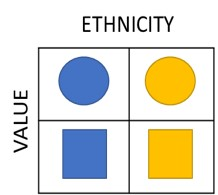
\includegraphics[width=0.3\textwidth]{material/figures/model.jpg}
    \caption{Agents type}
    \label{fig:model}
\end{figure}

In our model value orientation of agents is relevant for two reasons. First, it determines an additional dimension of similarity which is independent of ethnicity: liberals can recognize as similar value-oriented also liberals of the other ethnic group, so as to recognize of different value orientation conservatives of both ethnic groups\footnote{Equally, also conservatives recognize similar value-oriented conservatives of both ethnic groups}. Additionally, value orientation matters in defining the strength of ethnic or value similarity in the relocation decision of agents.
In \textcite{paolillo2018} agents randomly relocated to an empty node according to a threshold function, based on ethnic composition for ethnicity-oriented agents and value composition for value-oriented agents. We substitute this behavior with a binary random utility discrete choice model. At each time step, a random agent selects a random empty node and compares its neighborhood composition to that of its current node. By neighborhood of the agent we refer to the Moore neighborhood of radius 1 of the agent selected; similarly, the alternative neighborhood is the Moore neighborhood of radius 1 of an empty cell. We substitute the threshold function in \textcite{paolillo2018} with a continuous linear function for both ethnic and value neighborhood composition:

\begin{equation}
   U^e_j = \frac{x^e_j}{X_j} \quad\text{    ;   }\quad   U^v_j = \frac{x^v_j}{X_j}
\end{equation}

where:\\
$U^e_j$: ethnic utility of neighborhood j \\
$x^e_j$: number of agents in neighborhood j with same ethnicity \\
$X_j$: total number agents in neighborhood j\\
$U^v_j$: value utility of neighborhood j \\
$x^v_j$: number of agents in neighborhood j with same value \\
$X_j$: total number agents in neighborhood j\\

Both utilities can range [0,1]. Utility of a neighborhood is set to 0 if $X_j = 0$, i.e. not agents are in the neighborhood. The probability for an agent to choose the alternative neighborhood over the current one is modeled with a logistic function as:

\begin{equation}
    P_{al} = \frac{exp(\beta_e U^e_{al} + \beta_v U^v_{al})}{1 + exp((\beta_e U^e_{cr} + \beta_v U^v_{cr}) - (\beta_e U^e_{al} + \beta_v U^v_{al}))}
    \label{eq:lgst}
\end{equation}


where: \\
$\beta_e$: weight for ethnic preference \\
$\beta_v$: weight for value preference\\
$U^e_{al}$: ethnic utility of alternative neighborhood\\
$U^e_{cr}$: ethnic utility of current neighborhood\\
$U^v_{al}$: value utility of alternative neighborhood\\
$U^v_{cr}$: value utility of current neighborhood\\

The higher $\beta_e$ or $\beta_v$, the higher the option with higher ethnic or value utility is likely to be selected, the lower $\beta_e$ or $\beta_v$, the higher the chance that selection is random for that dimension. With both $\beta_e = 0$ and $\beta_v = 0$, the choice is totally random and $P_{al} = P_{cr} = 0.5$. This formula is a transformation of Eq: \ref{eq:cndtnl} for a binary choice with probability to relocate to alternative neighborhood\footnote{The equivalence between logistic function  and conditional logit for two options is valid since the difference between random terms that are assumed to have a Gumbel distributions has a logistic distribution. The logistic function in Eq: \ref{eq:lgst} is transformation of Eq: \ref{eq:cndtnl} written as $P_{al} = \frac{exp(U_{al})}{exp(U_{al}-U_{cr})}$, resulting from division of numerator and denominator by numerator $exp(U_{al})$, with $exp(U_{cr})/exp(U_{al}) = exp(U_{cr}) - exp(U_{al})$ (see \textcite[p.39]{train2009discrete} for detaills)}.
Probability computed is compared to a random number ranging between 0 and 1. If probability is higher than random number, then the agent moves to the alternative neighborhood, leaving its cell empty. So,  the logistic  function serves as a simplified version of the roulette wheel selection \footnote{see \textcite{bruch2012methodological} for an example of roulette wheel selection}.

We opted for a binary choice to ease computational power required. As tested, due to iterations of the model results would not change with selection between more options. We opted for a continuous linear function because default assumption in utility maximization and sensitive to changes in neighborhood compositions, which is strategic to our aim \autocite{van2009neighborhood}. Moreover, it lets behavior of agents differ only for parameters of determinism $\beta_e$ and $\beta_v$, so to allow us to disentangle the effect of either ethnic or value similarity preferences on emerging segregation. \rocco{next paragraph: I mean that potentially one can span the parameters so to have ethnic liberal > ethnic conservative. We impose preferences as I describe because of theoretical consistency with our research goal} We vary $\beta_e$ and $\beta_v$ depending on the value orientation of agents and in our experiments impose differences in heterogeneous preferences between the two types of agents. Liberal agents, considered as more  prone to ethnic tolerance, hold higher value preferences: weight for ethnic similarity cannot exceed their weight for value similarity ($\beta^{\ocircle}_v \geq \beta^{\ocircle}_e$). Conservative agents hold higher ethnic preferences: weight for value similarity cannot exceed their weight for  ethnic similarity ($\beta^{\Box}_e \geq \beta^{\Box}_v$). Moreover, the heterogeneity between conservative and liberal agents exists so that ethnic preferences of liberals do not exceed those of conservatives ($\beta^{\Box}_e \geq \beta^{\ocircle}_e$), and value preferences of conservatives do not exceed those of liberals ($\beta^{\ocircle}_v \geq \beta^{\Box}_v$).

As outcome of the model, we report the index of exposure for both ethnic and value segregation of agents who have at least one neighbor. This is the classic measure of segregation in Schelling and is equivalent to the fraction of agents of same ethnicity or value orientation in the neighborhood, indifferent to the actual number of neighbors. Nevertheless, we consider this a best fir to our interest in hybrid segregation scenarios. Since the measure is collected for all agents who have at least one neighbor, an index equal 0 means assimilation of the agent for that dimension, i.e. exposed only to agents of different ethnicity or value orientation. An index equal to 0.5 means that the agent is perfectly integrated for that dimension, being exposed to agents of different ethnicity or value orientation. An index equal 1 means total segregation, i.e. exposure only to similar agents for that dimension. Thus, the 2 indexes can be easily compared to visualize if agents are assimilated, integrated or segregated for one dimension and differently for the other.





\begin{table}[H]

\begin{tabular}{lll}
 \hline
\textbf{Agent definition}  & \textbf{Range}    \\ 
 \hline
 Ethnicity  (\textit{color})         & Blue (majority), Orange (minority)  \\
 Value orientation (\textit{shape}) & Square (conservative), Circle (liberal) \\
 Determinism ethnic utility ($\beta_e$) & $[0,\inf)$ 
 $\beta^{\Box}_e \geq \beta^{\Box}_v$
 $\quad\text{   ;    }\quad \beta^{\Box}_e \geq \beta^{\ocircle}_e$
 \\
 Determinism value utility ($\beta_v$) & $[0,\inf)$ $\beta^{\ocircle}_v \geq \beta^{\ocircle}_e$
 $\quad\text{   ;    }\quad \beta^{\ocircle}_v \geq \beta^{\Box}_v$\\
 \hline
\textbf{Global Parameters}  & \textbf{Range} \\ 
\hline 
 Population density      & $[0,0.99]$ \\
 Ethnic ratio majority/minority &  $[0,1]$ \\
 Value ratio conservative/liberal majority & $[0,1]$ \\
 Value ratio conservative/liberal minority  & $[0,1]$ \\
 \hline
 \textbf{Output measure}  & \textbf{Range} \\ 
\hline 
 Ethnic neighborhood exposure      & $[0,1]$ \\
 Value neighborhood exposure       & $[0,1]$ \\
 \hline
\end{tabular}
 \caption{Model parameters} 
 \label{tab:parameters}
\end{table}


\section*{Results}

We are interested in the segregation patterns emerging from the interaction of ethnic and value homophily preferences of agents and their varying degree of determinism. To this aim, we report only the final results of our simulation runs collapsed on the average. We repeated each parameter setting for 20 runs and each run lasted 2000 discrete time steps, which was enough to let agents reiterate their decision and stable equilibria occur. In Annex B, we report a robustness analysis for each parameter setting. In this first section we focus on a symmetric condition where each group-type % due to intersection of ethnicity and value-orientation
represents $25 \%$ of the global population. Fig. \ref{fig:space} shows the parameter space we explore in this baseline scenario and the figures associated. 

\rocco{I shifted here from model section} As measure of segregation, for both ethnic and value similarity, we compute an index of exposure in the Moore neighborhood of agents who have at least one neighbor. The index reports % on average 
the fraction of other agents of same ethnicity or same value orientation in the local neighborhood of each agent. An index of 0.5 equals to integration between the two groups, an index equal 1 corresponds to full segregation. We report the index for ethnic exposure ($E_i$) and value exposure ($V_i$) for each group-type:

\begin{equation}
   E_i = \frac{x^e_i}{X_i}\quad\text{   ;    }\quad  V_i = \frac{x^v_i}{X_i}
\end{equation}

where:\\
$x^e_i$: number of other co-ethnic agents in the Moore neighborhood of agent i\\
$x^v_i$: number of other co-value  agents in the Moore neighborhood of agent \textit{i}\\
$X_i$: total number agents in neighborhood of agent \textit{i}\\


\begin{figure}[h]
    \centering
    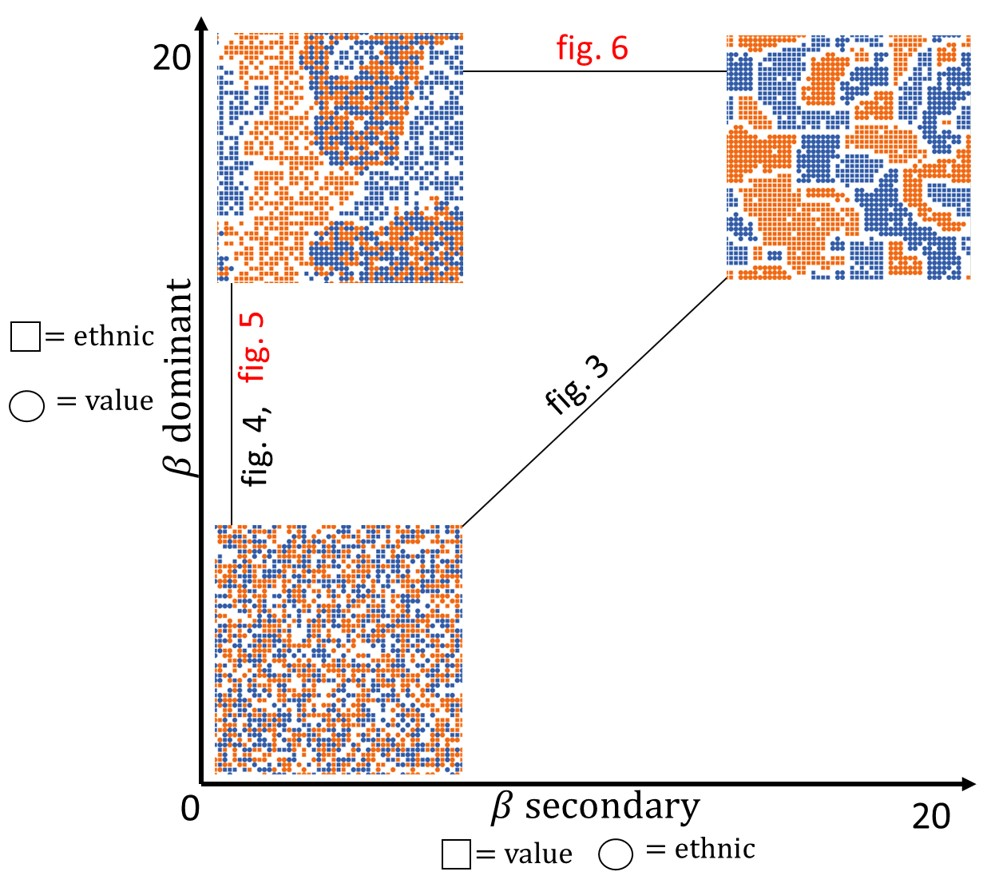
\includegraphics[width=1\textwidth]{material/figures/model_space.jpg}
    \caption{Space Model. Black color figures: same degree of determinism for all agents; Red color figures: different degree of determinism for liberal and conservative agents}
    \label{fig:space}
\end{figure}

Fig: \ref{fig:baseline} moves along the diagonal in Fig: \ref{fig:space}, with agents increasing simultaneously value and ethnic preferences, meaning they want to live close to other agents of the own group-type. X-axis shows the increase in preference determinism, while y-axis reports the segregation as measured with the exposure index\footnote{We report x-axis until $\beta \, dominant = \beta \, secondary = 20$ since the stability of the model is evident. From other observations in the verification phase of the model we observed no changes for higher levels of $\beta$}. We use this as the baseline scenario we compare other conditions to. % Since each group-type is equally represented and agents hold the same preferences, the curve of segregation is the same for each group-type. 
With $\beta \, dominant = \beta \, secondary = 0$ no segregation occurs due to random  relocations. Then segregation increases monotonically until equilibrium is reached with complete segregation at $\beta \simeq 7$. 

\begin{figure}[H]
  \centering
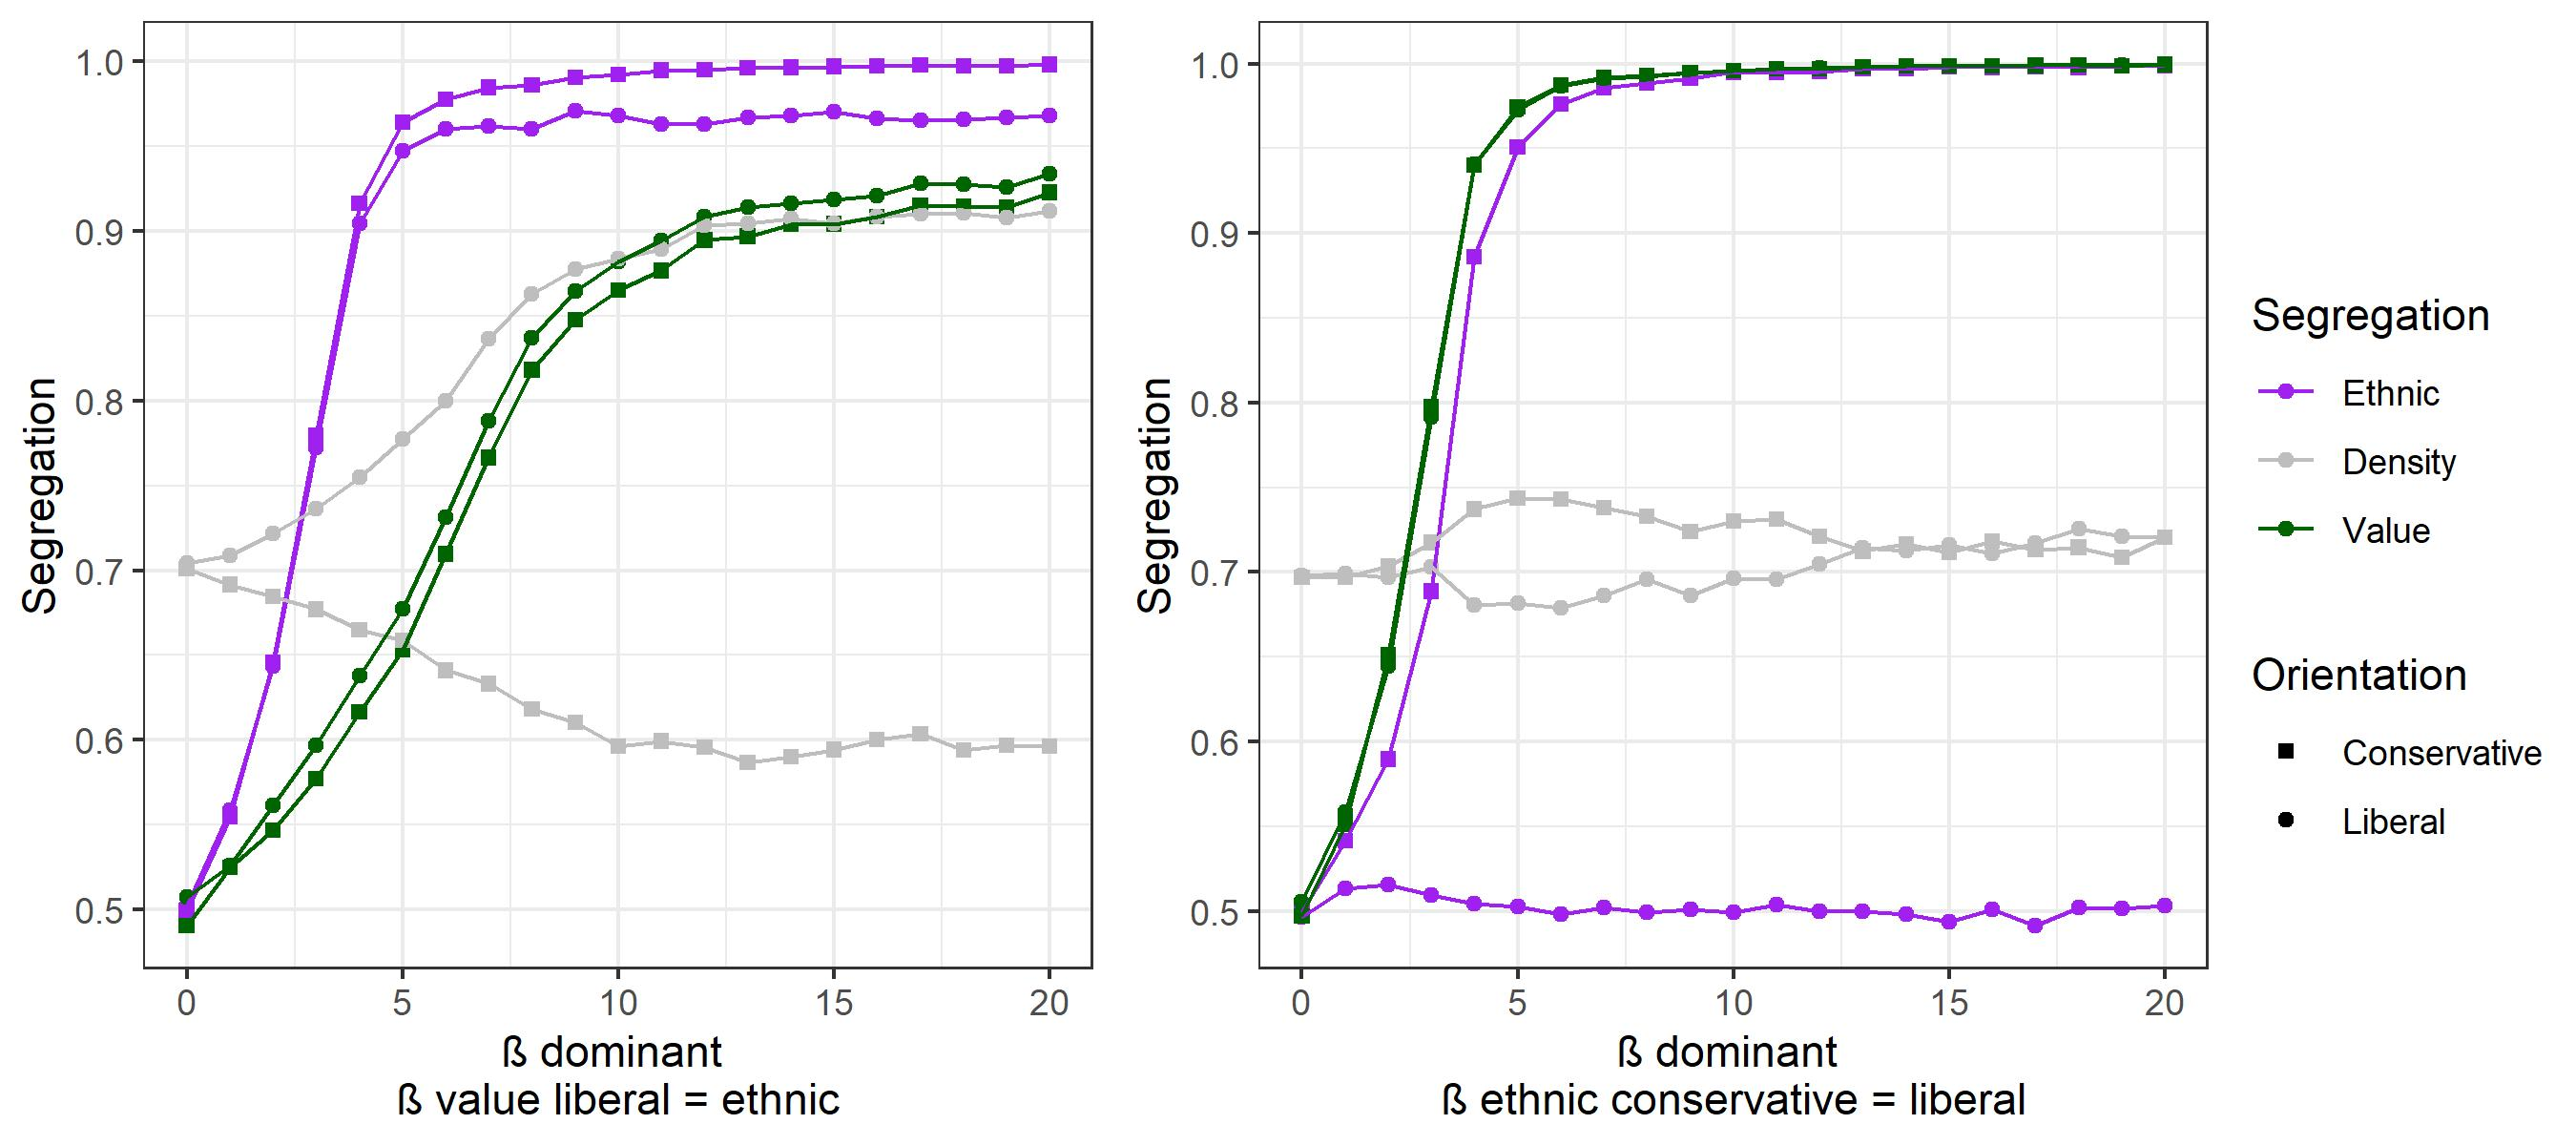
\includegraphics[scale=0.6]{material/figures/Bsl_eth_lib.jpg}
    \caption{testing other pics}
    \label{fig:testing pics}
\end{figure} % baseline


\begin{figure}[H]
    \centering
    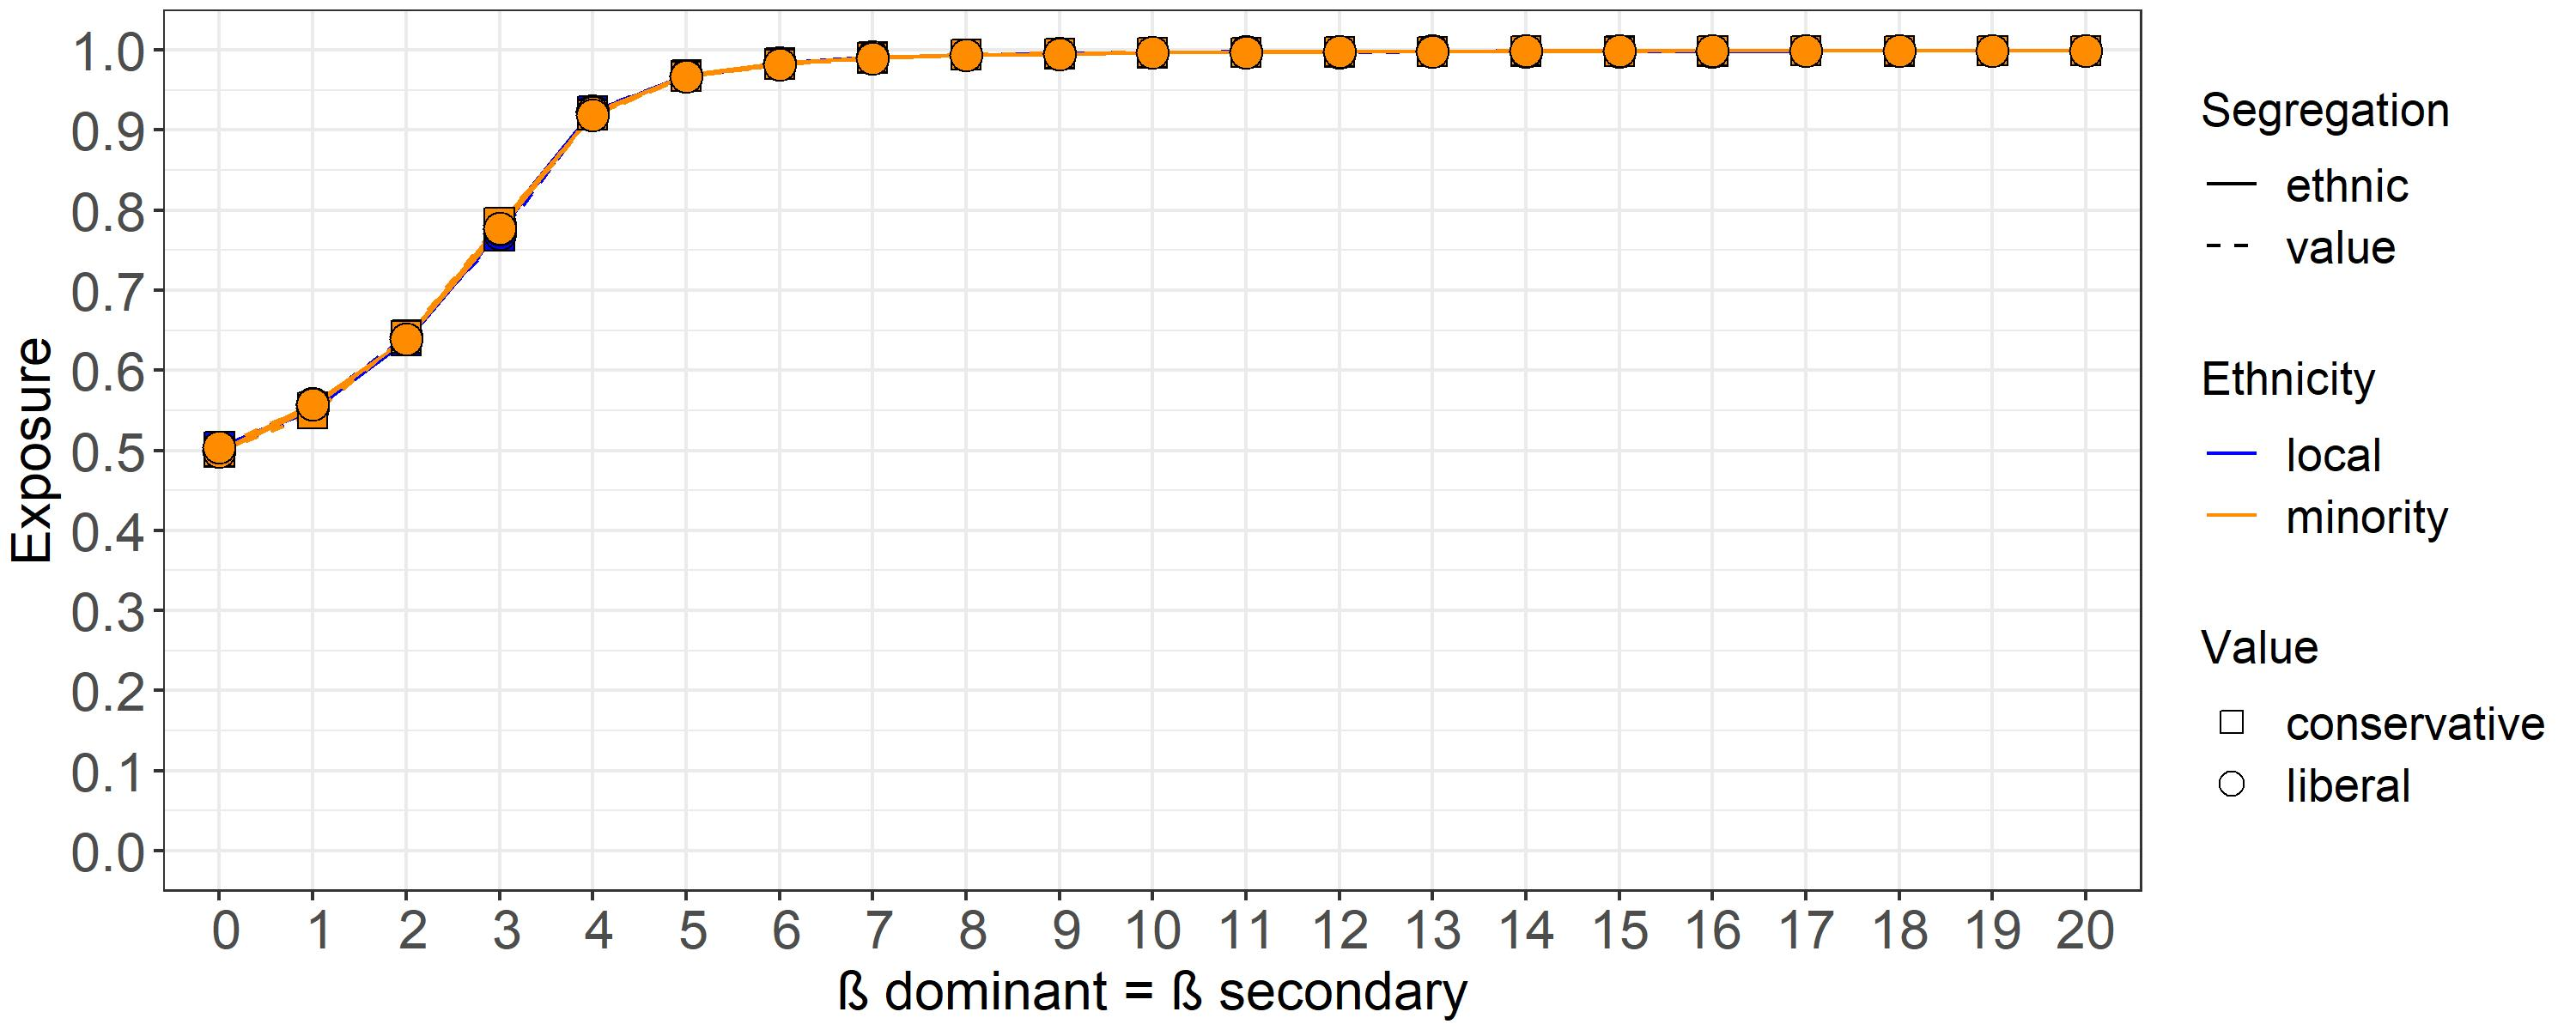
\includegraphics[scale=0.5]{material/figures/one_beta.jpg}
    \caption{Baseline scenario. Each of the 4 agent types represents $25 \%$ of the population. $\beta_{dominant} = \beta_{secondary}$}
    \label{fig:baseline}
\end{figure} % baseline
 
Fig: \ref{fig:sec_0} shows the case where agents only hold to their dominant preference and not care about secondary preference %, i.e. conservative agents care about neighborhood ethnic composition and not about value, while liberal agents care about neighborhood value composition and ignore its ethnic composition.
, so to observe dynamics not evident in Fig: \ref{fig:baseline} due to double-segregation. \rocco{This was also the main scenario in \textcite{paolillo2018} we translate in discrete choice and random utility}
Stable segregation now occurs at higher level of determinism $\beta \simeq 10$. Ethnic segregation of conservative agents is slight higher than value segregation of liberal agents for $\beta \leq 10$. While value segregation of liberals emerges with increase in their value preference, they remain ethnically integrated. This is the result of random relocations for ethnic dimension ($\beta^{\ocircle}_e = 0$) from even distribution and equal groups size. For conservative agents, as ethnic segregation increases due to ethnic preference, also value segregation increases. This result is counter-intuitive given that conservative agents do not care about value similarity. We refer to this condition as an example of hybrid segregation: some members of the same ethnic group (liberals) are ethnically integrated and segregate over the value dimension, while the others (conservative) experience both ethnic and value segregation. We want to delve into this mechanism with Fig: \ref{fig:comb_val} and Fig: \ref{fig:comb_sec}. 

\begin{figure}[H]
    \centering
    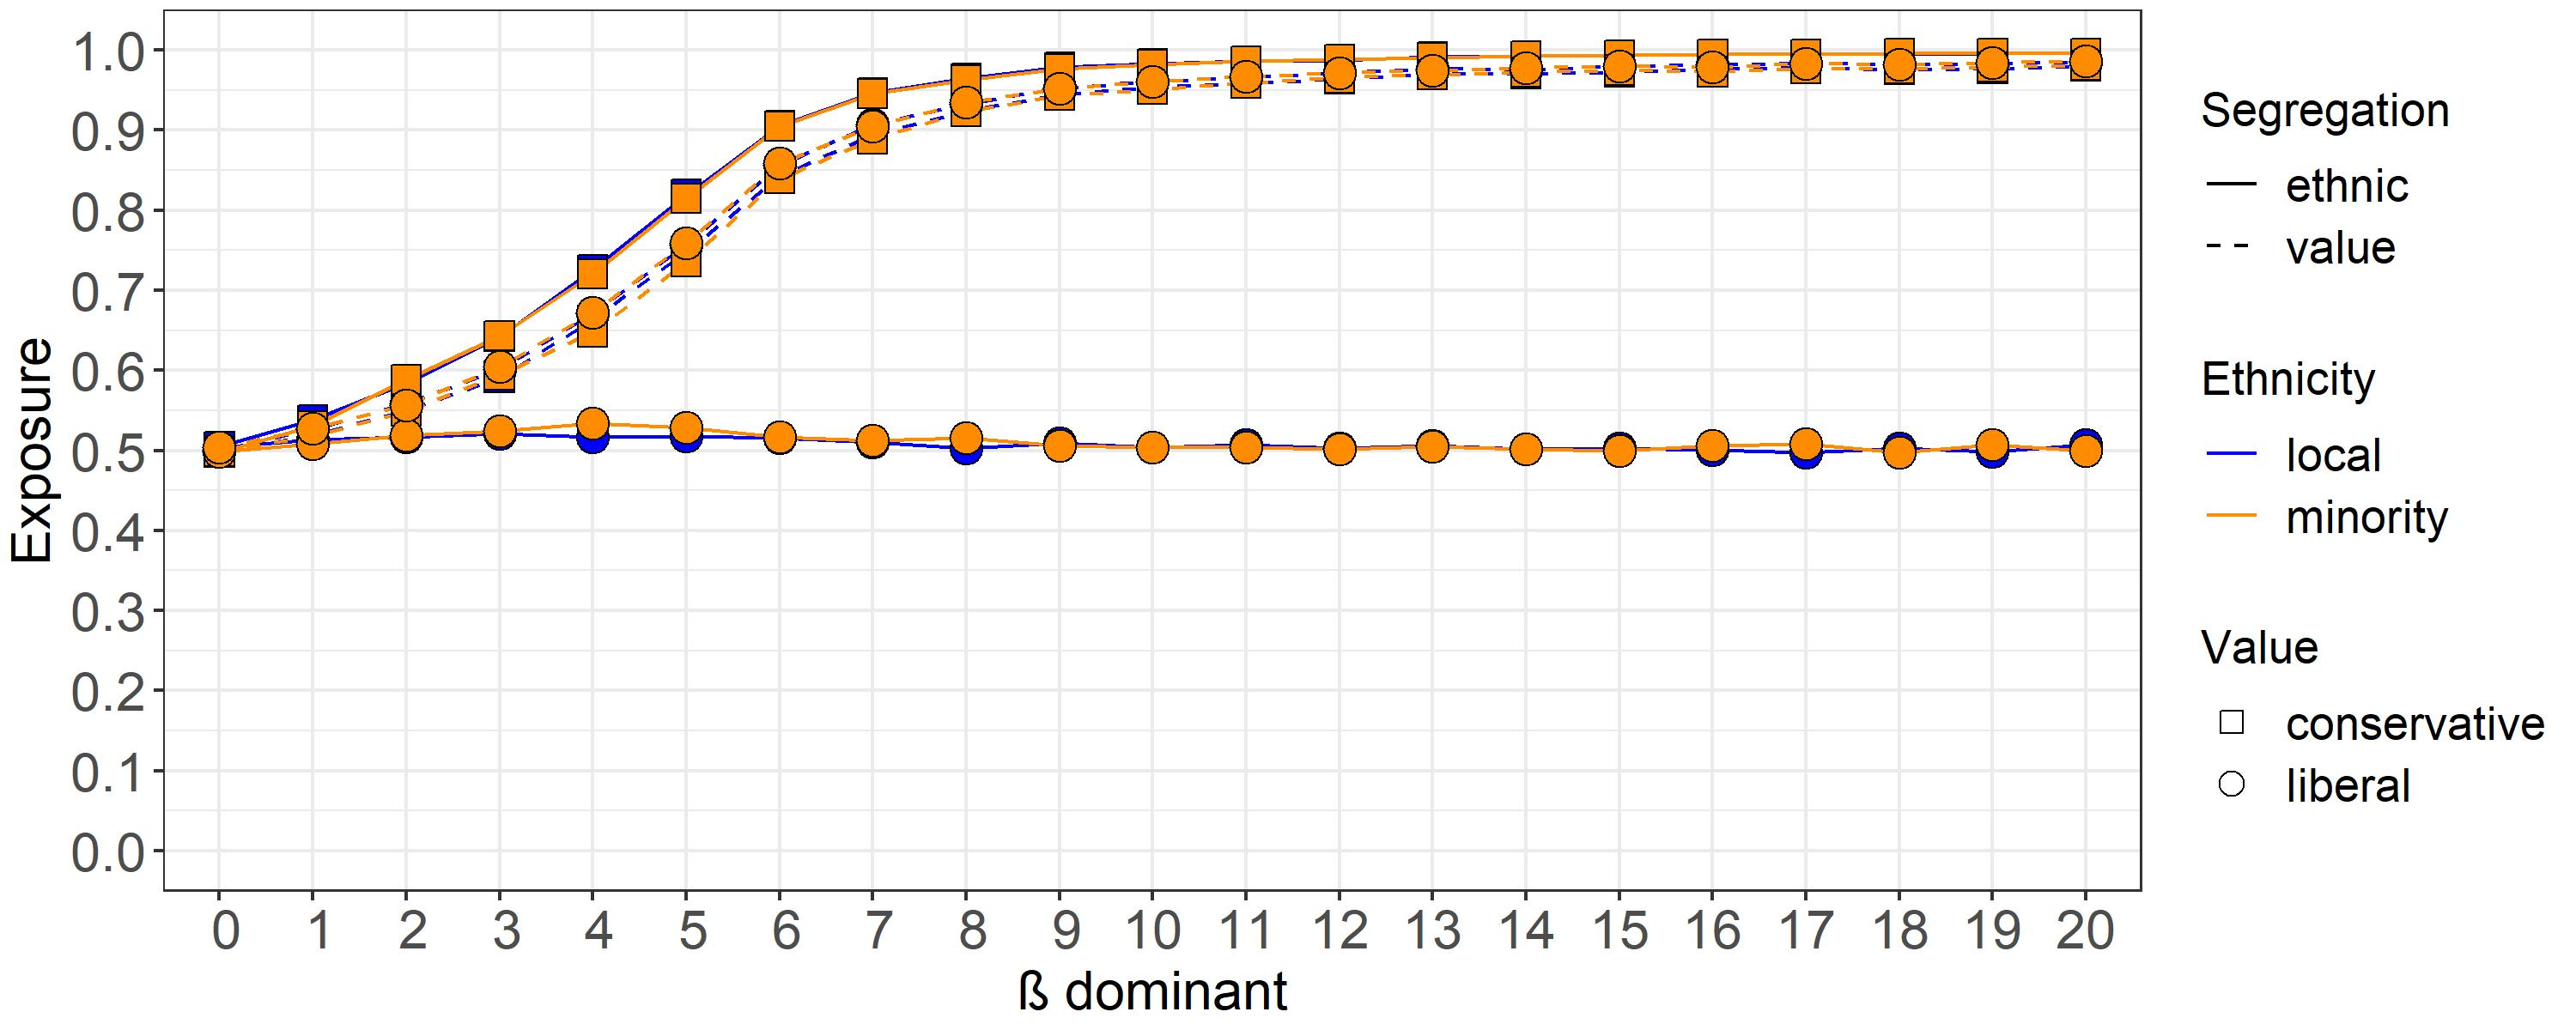
\includegraphics[scale=0.5]{material/figures/sec_0.jpg}
    \caption{Random secondary preference: liberal ethnic $\beta^{\ocircle}_e = 0$, conservative value $\beta^{\Box}_v = 0$}
    \label{fig:sec_0}
\end{figure} % secondary 0


\rocco{I thought and would like to give a try for the rest of basic section: one pic behavior of liberals  (combined top panel \ref{fig:comb_val} with the heatmap referred only to liberals) and conservatives (combined bottom panel \ref{fig:comb_val} with the heatmap referred only to conservatives). This means we simplify and show the effect of dominant preference of each (while others have dominant and secondary $\beta=0$, and until what extent increase in secondary preference can affect segregation while other hold to dominant preference}
 
Fig: \ref{fig:comb_val} decomposes Fig: \ref{fig:sec_0}, increasing dominant preference of either liberals (top panel) or conservatives (bottom panel), while other agents in each condition relocate randomly with $\beta = 0$. The graph shows how increase in value preference of liberals best reproduces the behavior of Fig: \ref{fig:sec_0}, with increase in value segregation of both liberals and conservatives, while agents remain ethnically integrated. % This is coherent with ethnic preference of all agents equal 0, but not with the value preference of conservatives also equal 0. 
With increase in ethnic preference of conservative agents (bottom panel), their ethnic segregation increases with a flatter curve than Fig: \ref{fig:sec_0} and reaching lower ethnic segregation at $E_i = 0.8$. % In short, Fig: \ref{fig:comb_val} shows how value segregation of conservative agents occurs as by-product segregation of value preferences of liberals.
As determinism of liberals increases, they will select those neighborhoods that maximize value utility so to eventually reduce their relocations to alternatives and form denser clusters. By doing so, they reduce the space on the lattice where conservative agents avoided because of different value orientation can randomly relocate, so that conservatives are forced into value segregation. In Fig: \ref{fig:sec_0}, differently from Fig: \ref{fig:comb_val}, conservative agents would relocate taking also ethnic homophily into account, so that they would select a co-ethnic necessarily of same conservative value orientation. Ethnic homophily of conservative agents does not produce the same effect. Moreover, in Fig: \ref{fig:comb_val} despite the same increase in determinism, the level of value segregation of liberals is higher than the level of ethnic segregation of conservatives. As both types of agents would consider half of the overall population as similar, %(the population is equally split into two ethnic groups and into two value orientations), 
the same degree of segregation should be theoretically expected. The different levels of segregation are due to the definition of similarity based on shared values or ethnic membership. In Fig: \ref{fig:comb_val}, though conservatives would satisfy their preference by living close to co-ethnics, not matter their value-orientation, liberals would relocate anyway. 
% Until here %
As such, though half of the population would be considered as similar by conservatives, they can rely only on co-ethnics that are also other conservatives to maximize ethnic utility, i.e. $25 \%$ of the population. On the contrary, liberal agents would relocate close to other liberals indifferent of ethnic membership, so that the entire $50 \%$ of the population is available to maximize value utility. The result is a tendency for liberals to form one macro neighborhood ethnically integrated and value homogeneous. This condition has also another consequence: because of the linear utility function, agents are more sensitive to change in neighborhood composition, so that agents who are on the border of a neighborhood would be more subject to the random relocations of others due to consequence these can have on utility of the current neighborhood. Following this reasoning, liberals in Fig: \ref{fig:comb_val} who form denser neighborhoods and live in the inner region of the neighborhood would be less subject to random relocations of conservatives. For conservatives who form smaller neighborhoods, more of them would be subject to random relocations of liberals of both ethnic groups, so to have higher chance to relocate due to fluctuations in the utility of the current neighborhood. This could be an additional explanation of the lower ethnic segregation of conservatives in Fig: \ref{fig:comb_val} compared to value segregation of liberals. In Fig: \ref{fig:sec_0}, similar dynamics occur, though they are reinforced by the self-clustering of agents by value or ethnic preference.

\begin{figure}[H]
    \centering
    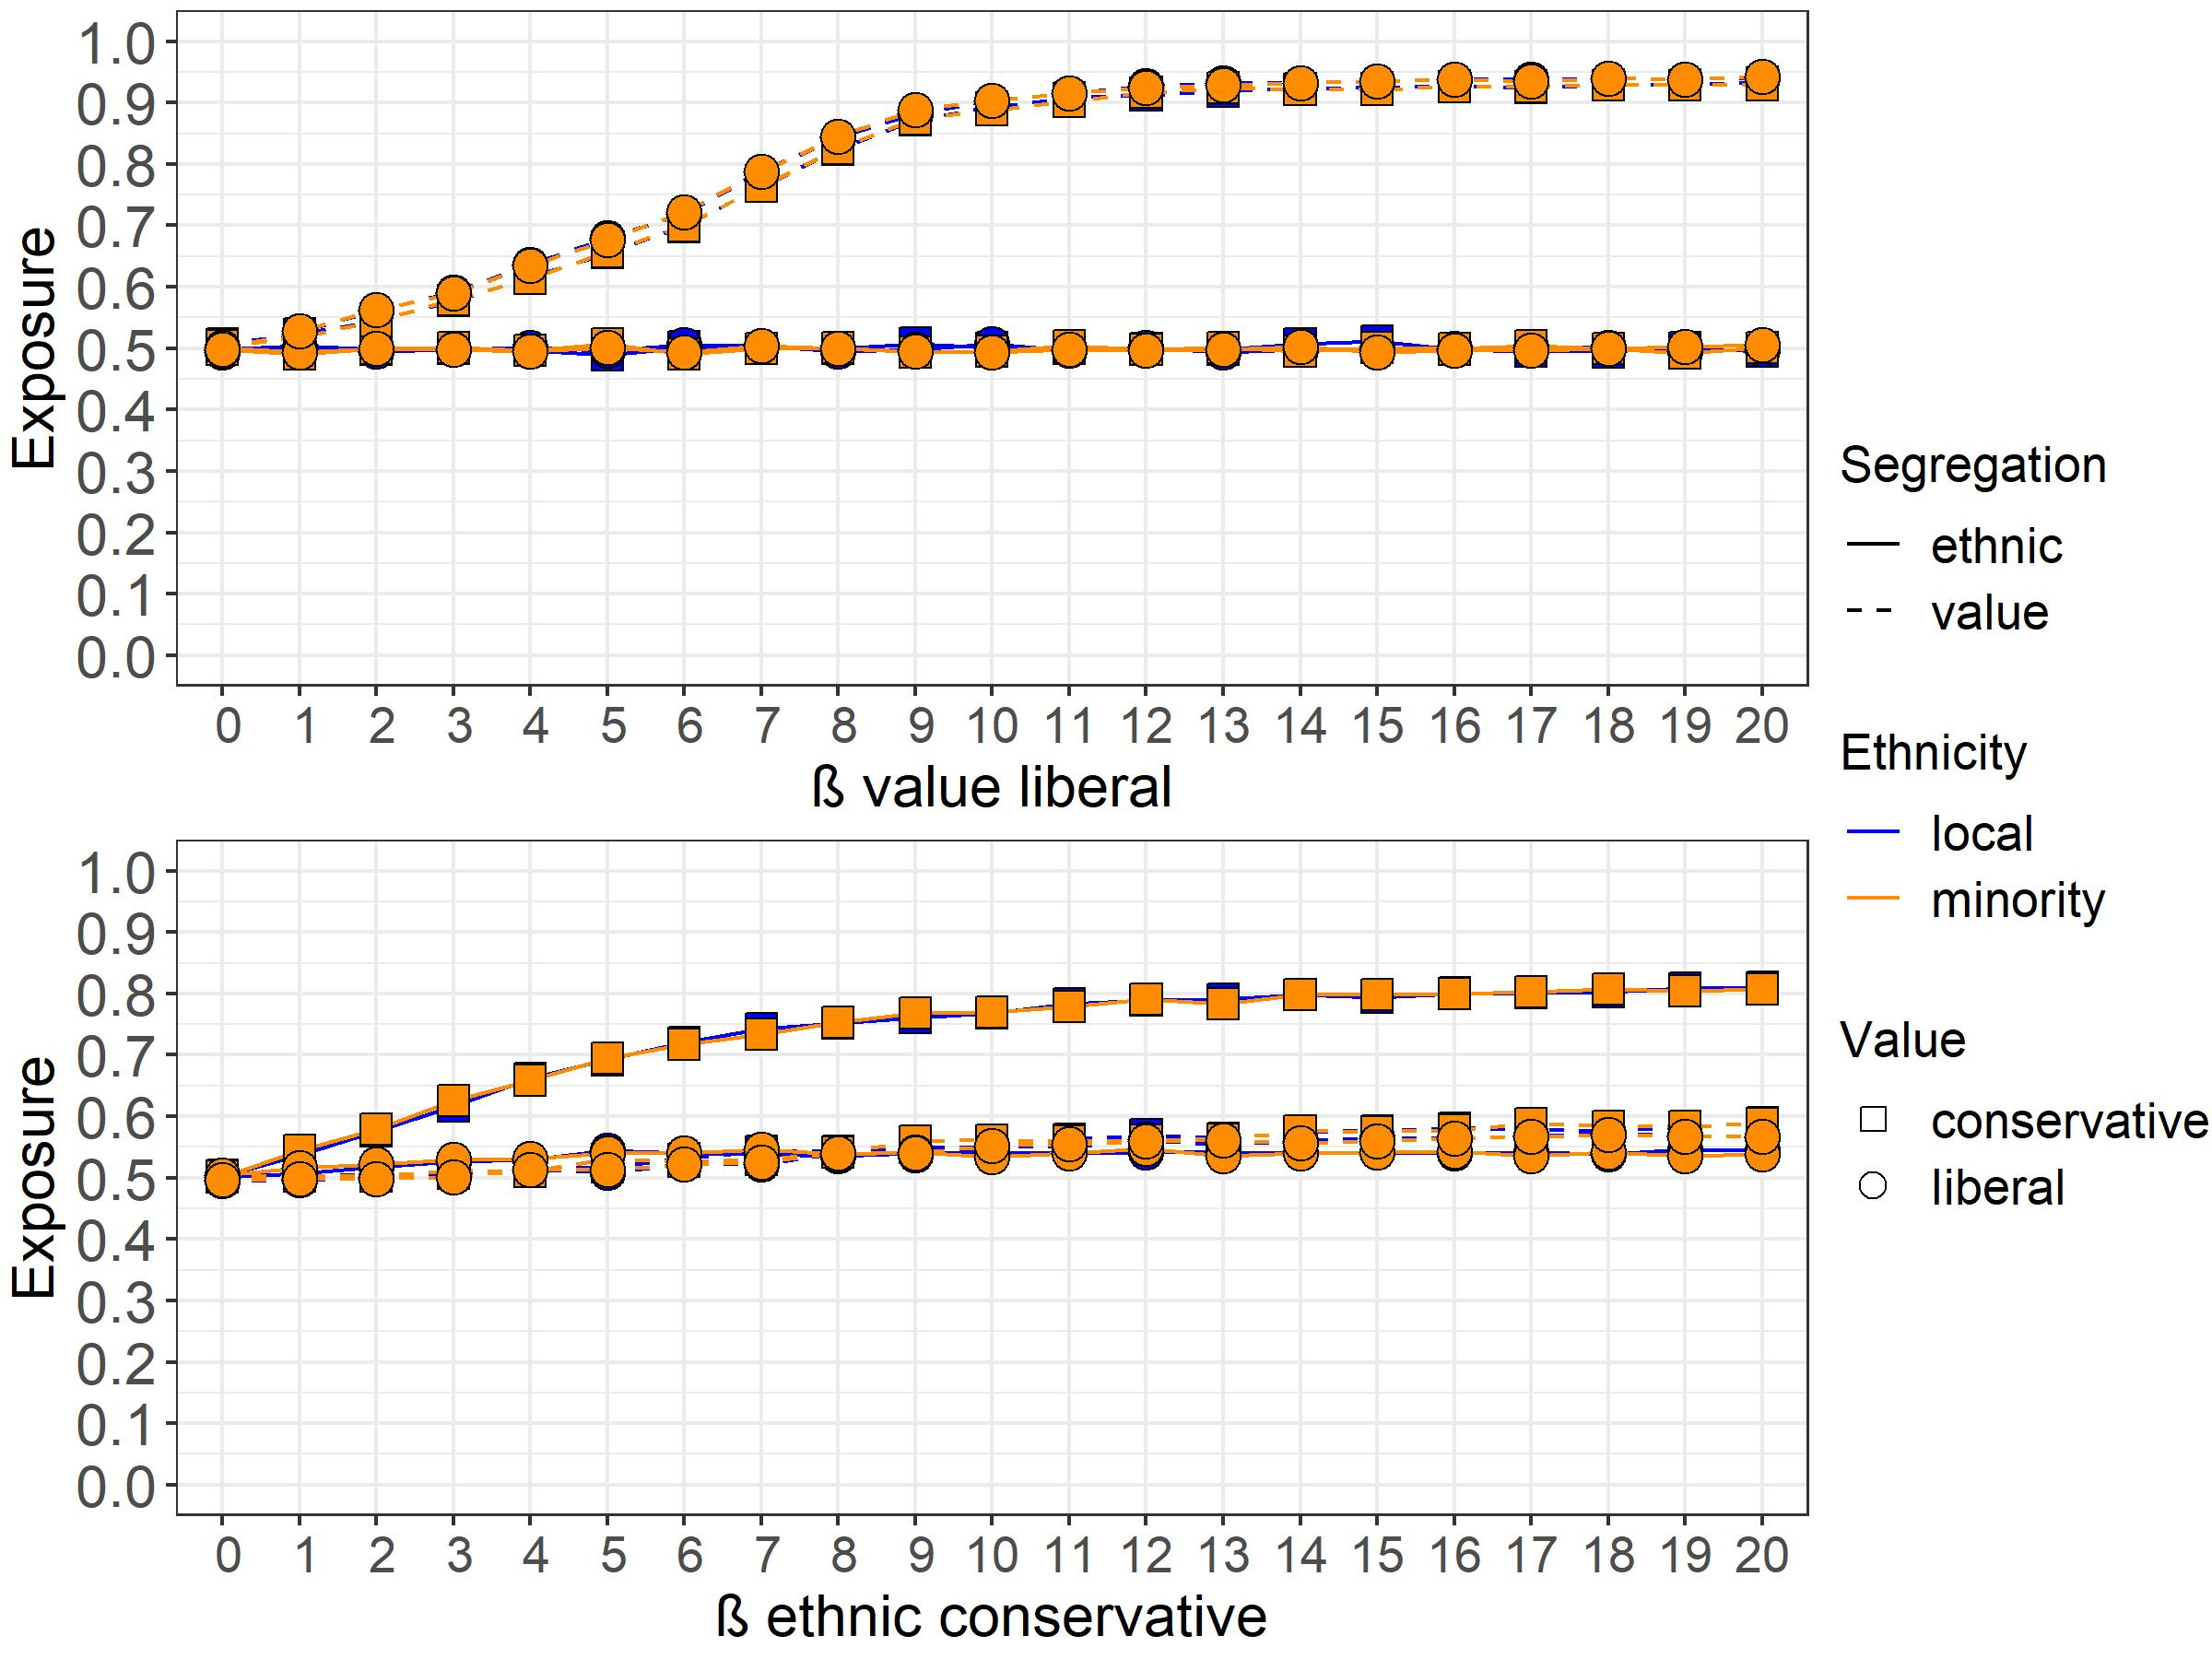
\includegraphics[scale=0.5]{material/figures/comb_val.jpg}
    \caption{Sensitivity to dominant preference by value orientation. Top: liberal value homophily $\beta^{\ocircle}_v$; Bottom: conservative ethnic homophily $\beta^{\Box}_e$. In each graph, all dominant and secondary preference of other agents are set equal to 0}
    \label{fig:comb_val}
\end{figure} % both value

In sum, similarity based on shared values compared to similarity based on ethnic membership has three effects: first to cause a by-product value segregation of conservative agents who do not care about value similarity, and secondly to form denser neighborhoods due to inclusion of co-values from both ethnic groups, and stemming from it higher resilience against fluctuations in neighborhood composition. Fig: \ref{fig:comb_sec} tests the assumptions we can deduce from Fig: \ref{fig:comb_val} in a scenario where each group-type increases both type of preferences: all agents hold $\beta \, dominant = 20$, with increase of either secondary ethnic preference  of liberals (top panel) or value preference of conservative (bottom panel) \rocco{for easiness would be good to combine Fig: \ref{fig:comb_val} and Fig: \ref{fig:comb_sec}}. When liberal agents increase their ethnic preferences, ethnic segregation increases linearly as expected, reproducing a scenario most similar to baseline Fig: \ref{fig:baseline} at $\beta \simeq 12$ instead of $\beta \simeq 7$, associated with slight decrease in value segregation for all agents due to new clusters formed. With increase in value preference of conservative agents, there are no changes in results, because the value segregation of conservative agents already emerges as by-product of high value preferences of liberal agents who remain ethnically integrated. Finally, the heatmap in Fig: \ref{fig:heatmap} shows other areas of the model space in Fig: \ref{fig:space} we have not explored and summarizes our results where liberals and conservatives hold the same degree of determinism. Along the diagonal (baseline: Fig: \ref{fig:baseline}), integration remains from even distribution for $\beta = 0$, then double segregation monotonically increases and stabilizes with complete segregation at $\beta \simeq 7$. When dominant preferences increase and secondary preferences remain random (Fig: \ref{fig:sec_0}), differences between liberals and conservatives become evident: liberals remain ethnically integrated, while value segregation emerges for both groups. Focusing on $\beta \, dominant = 20$, ethnic segregation of liberal agents emerges as secondary preference increases, while complete value segregation is stable; for conservatives, both full ethnic and value segregation remain constant and complete.





\begin{figure}[H]
    \centering
    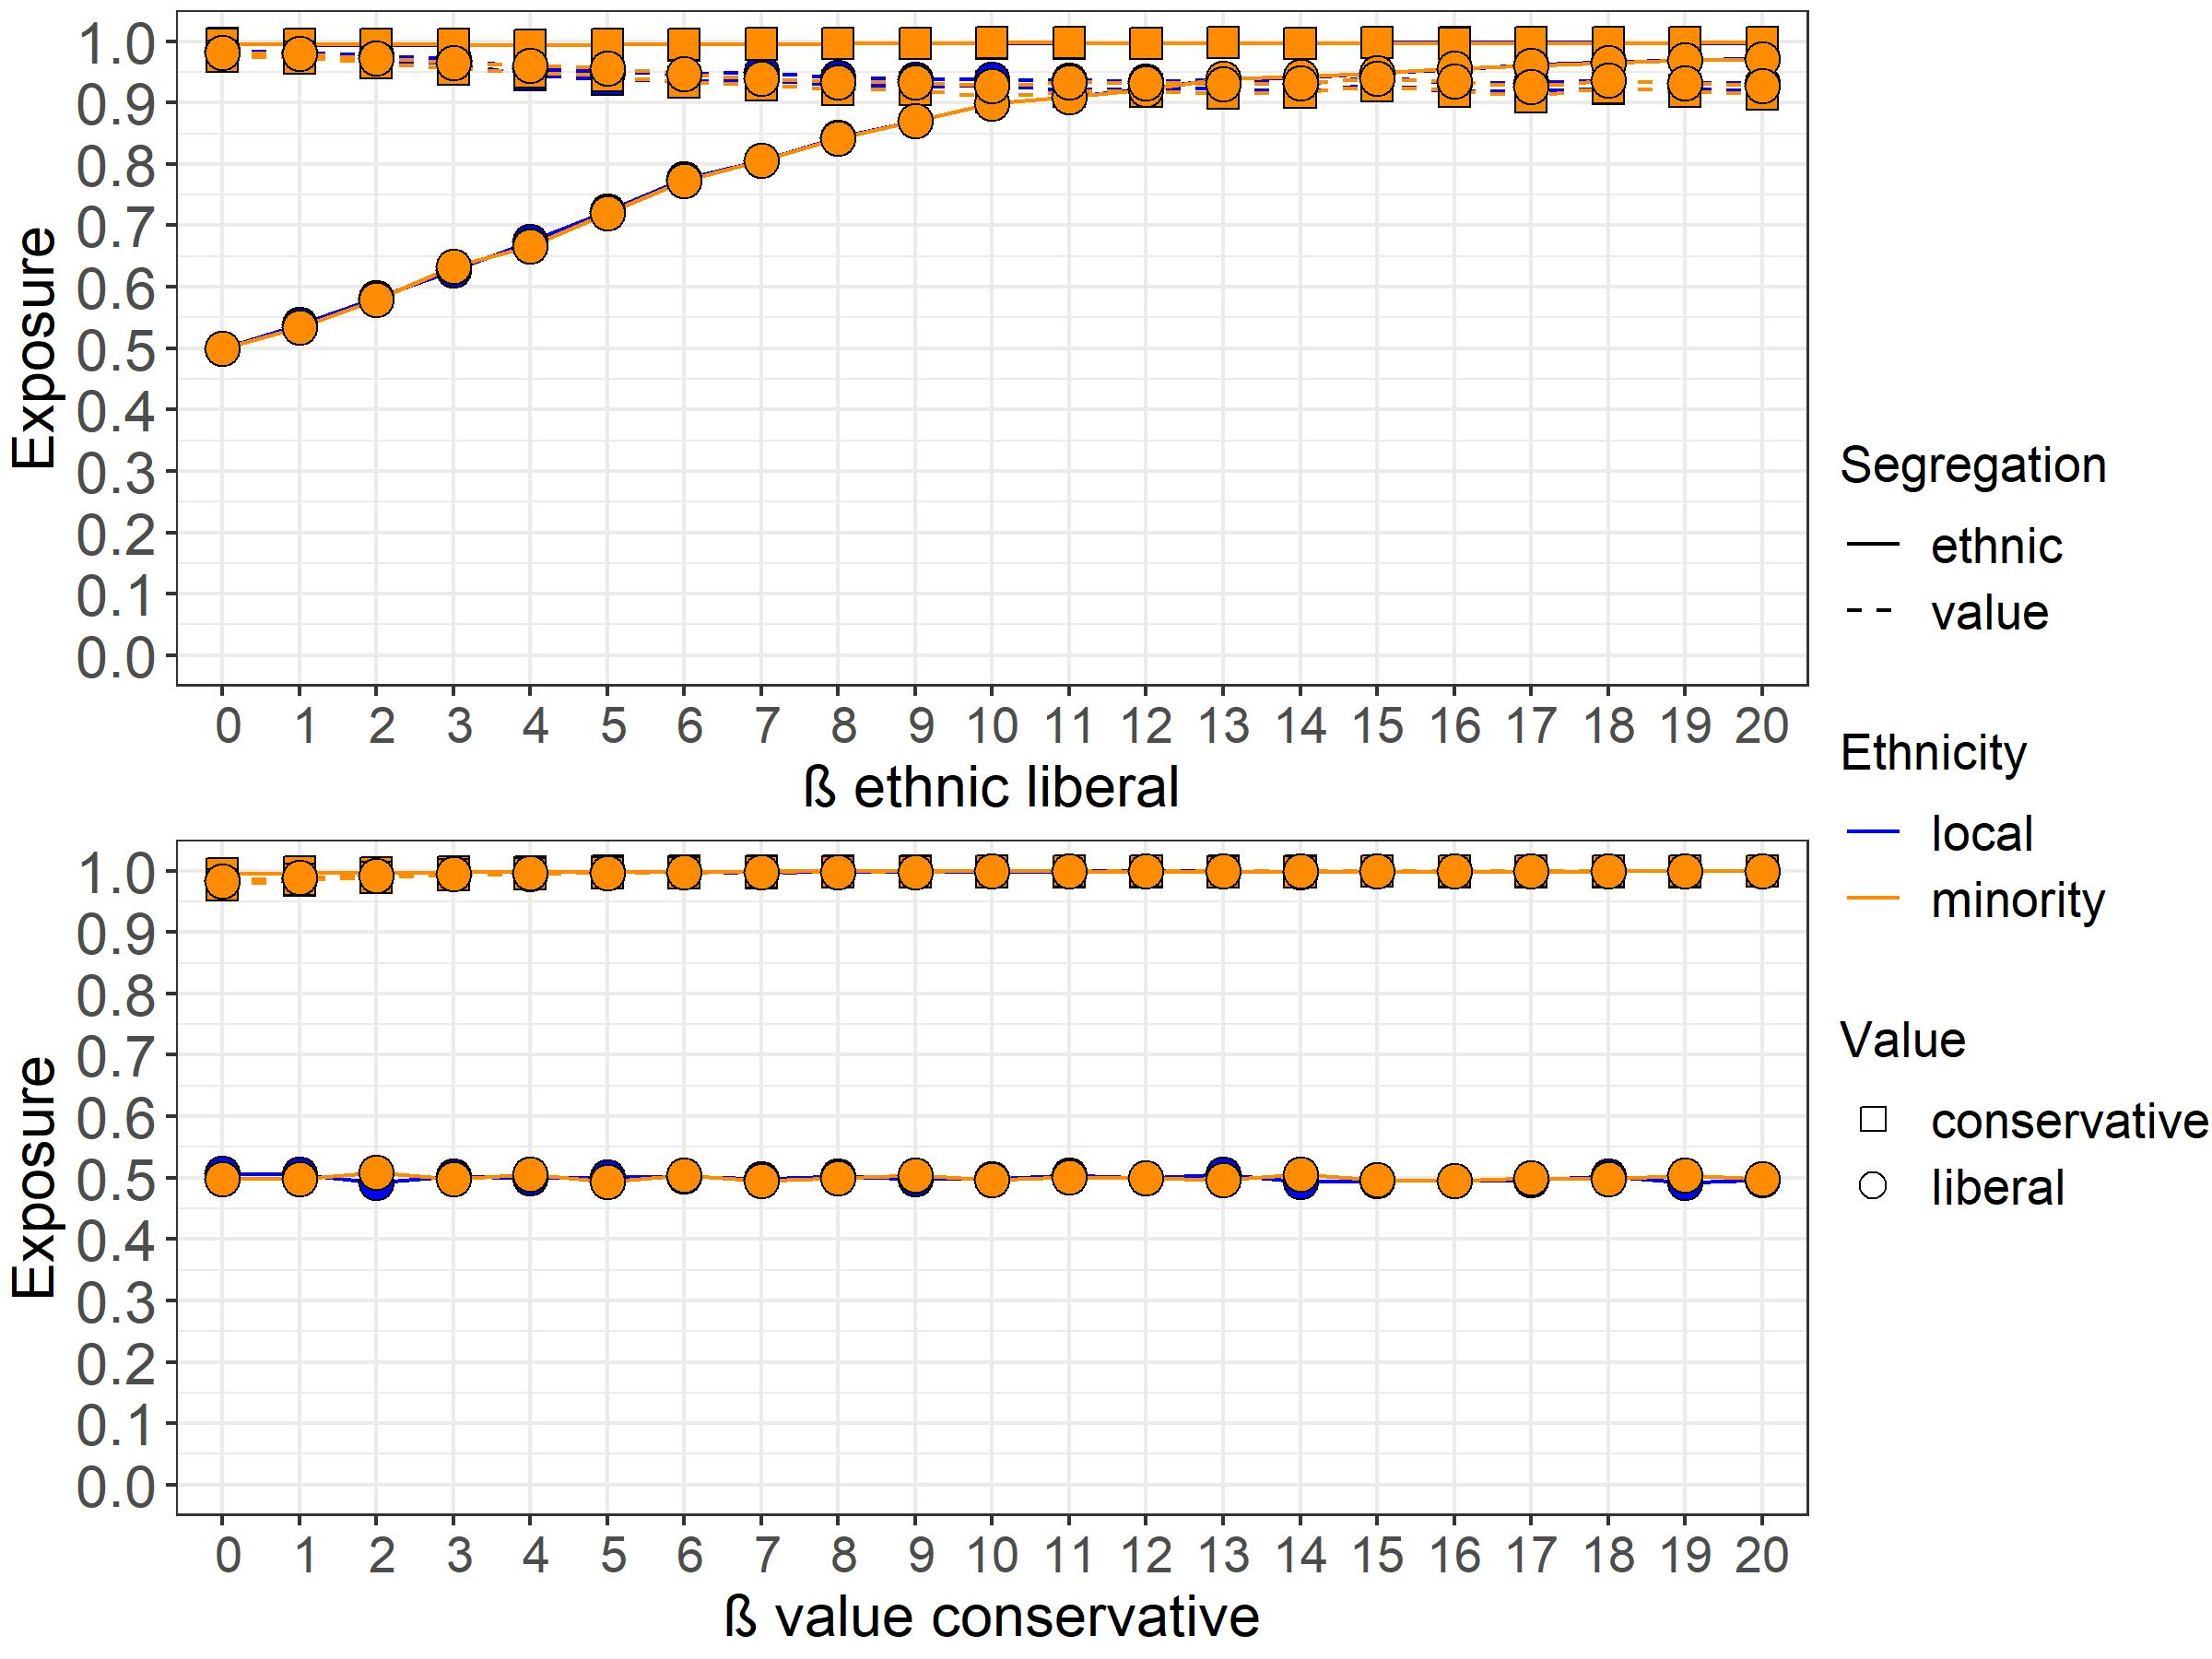
\includegraphics[scale=0.5]{material/figures/comb_sec_bln.jpg}
    \caption{Increase in secondary preference of liberals (top) and conservatives (bottom)}
    \label{fig:comb_sec}
\end{figure} % both secondary



\begin{figure}[H]
    \centering
    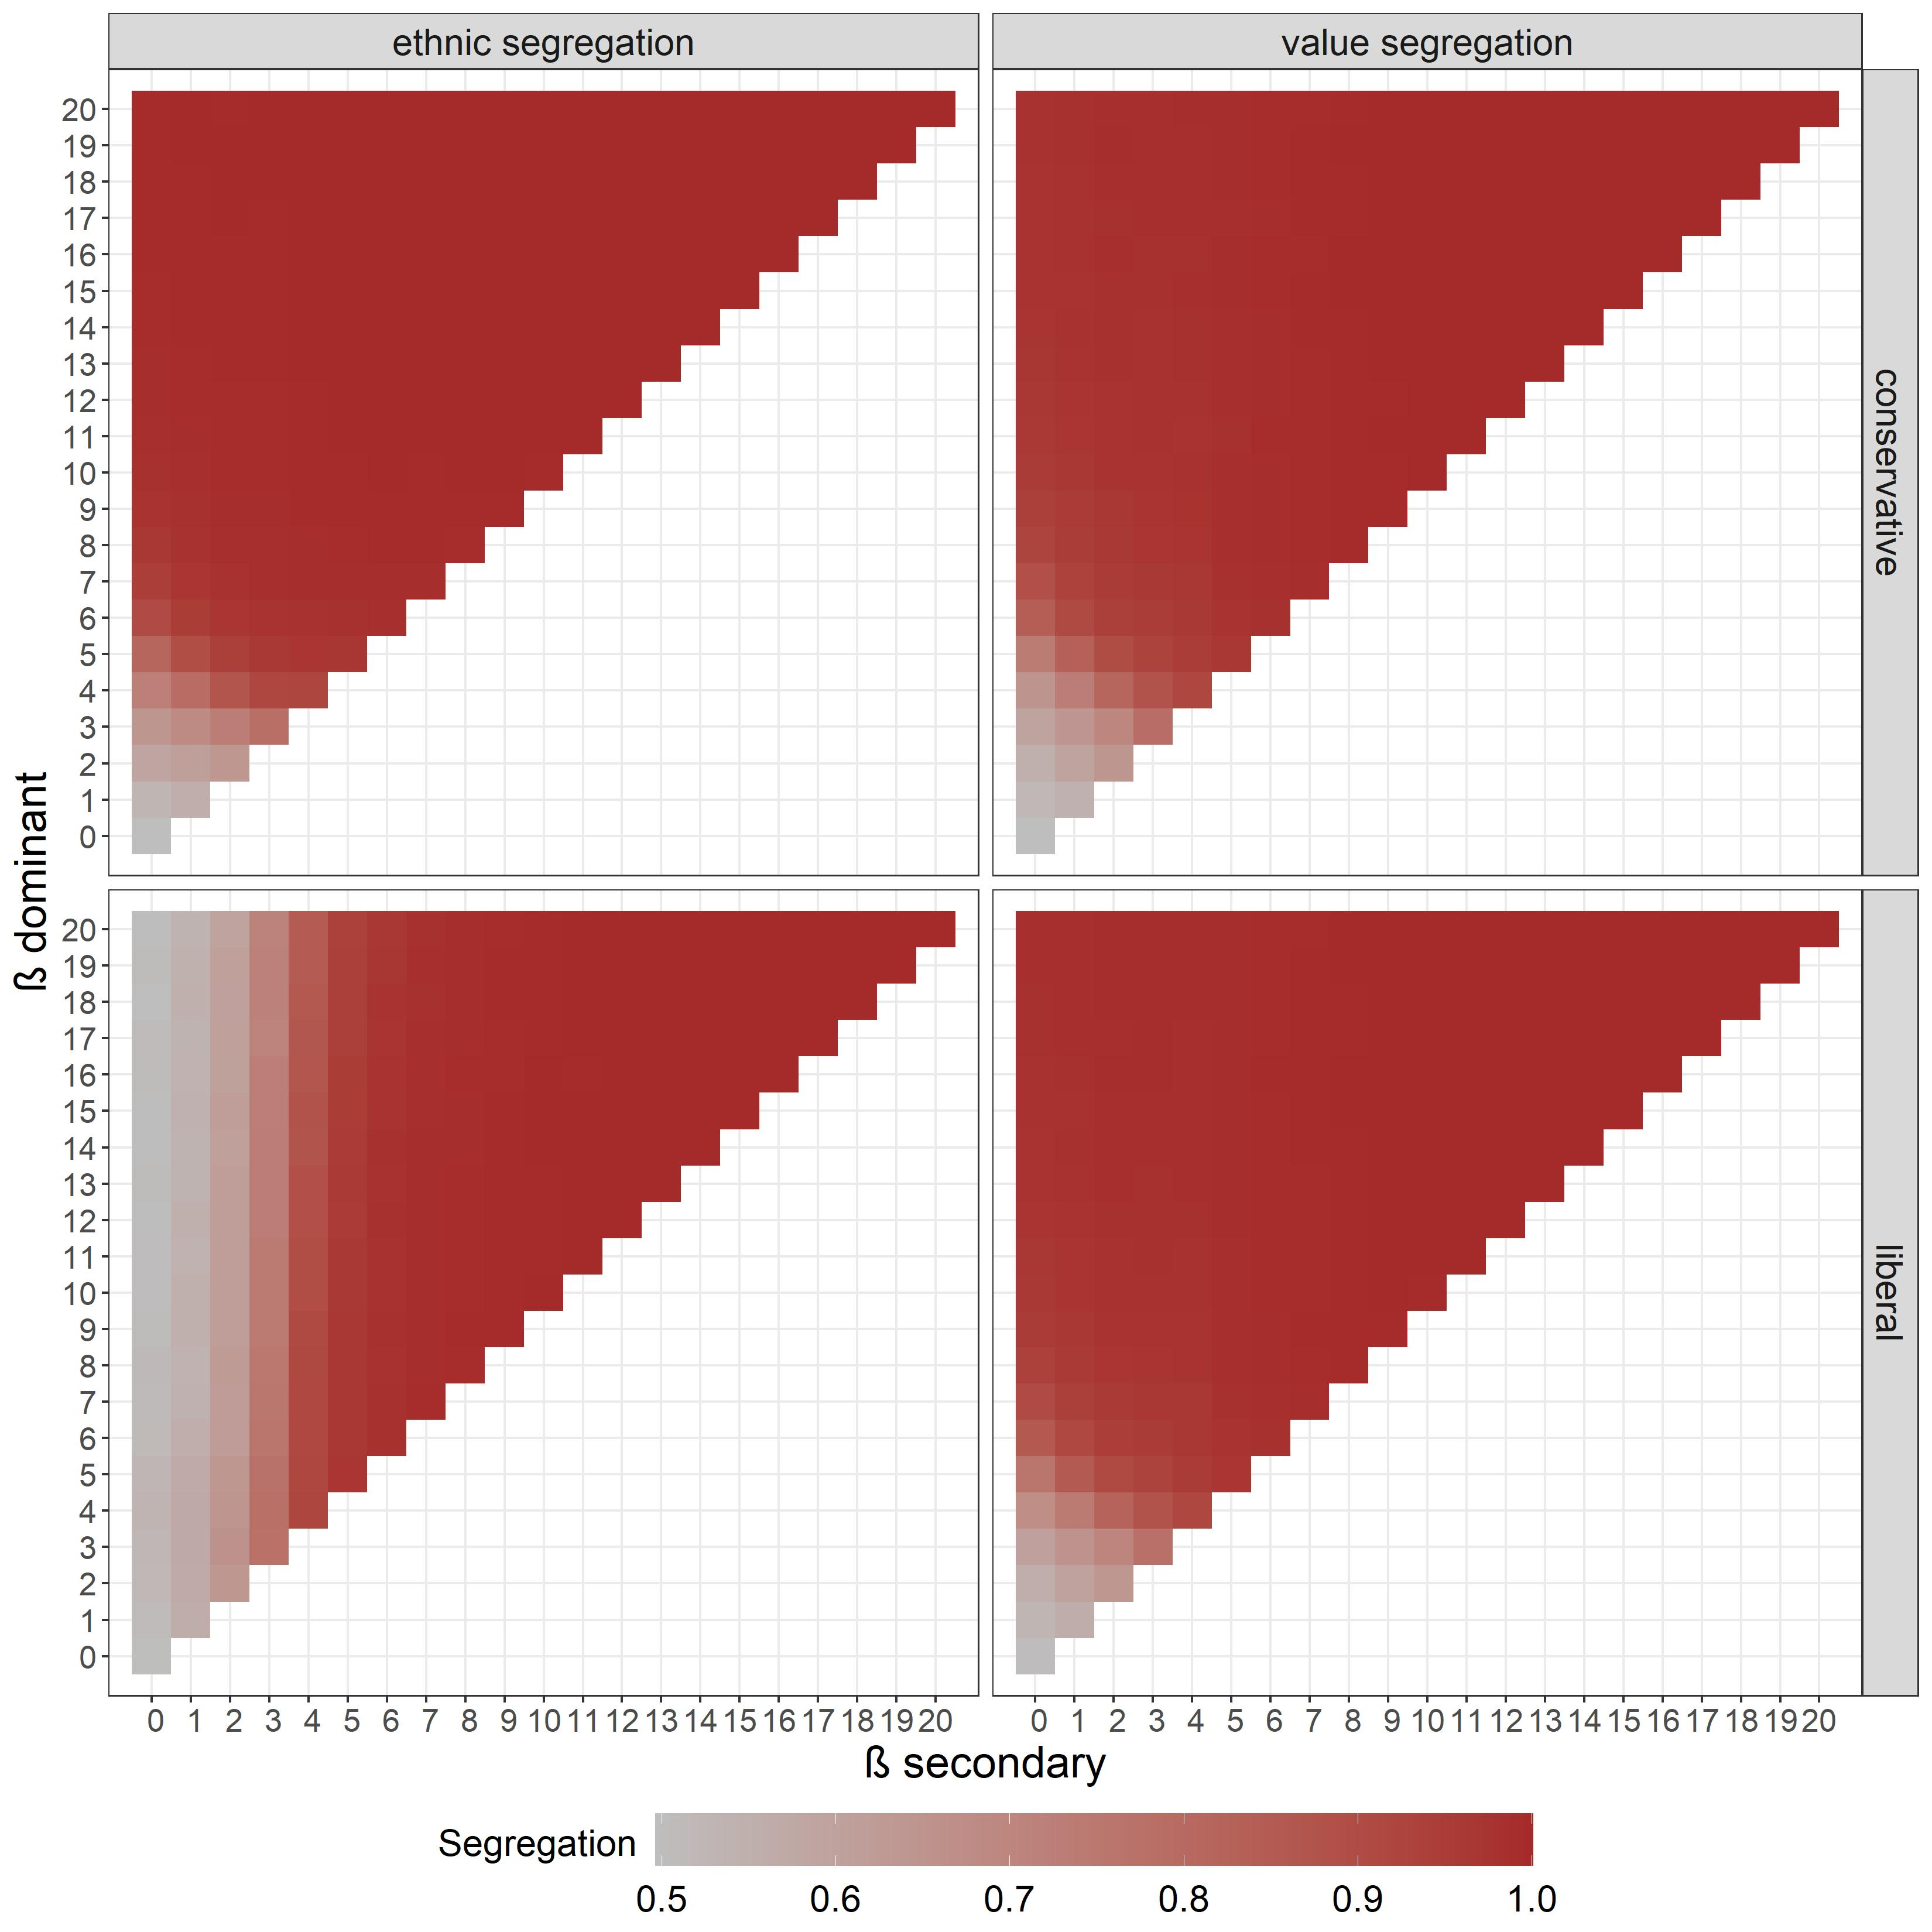
\includegraphics[width=0.9\textwidth]{material/figures/heatmapbase.jpg}
    \caption{Heatmap baseline dominant and secondary preference}
    \label{fig:heatmap}
\end{figure}


\section*{Asymmetric conditions}

\rocco{I have been collecting other conditions; text and figures from Fig. 10 might change/be substitute. Other conditions are to better investigate how preference of same value-type but belonging to either majority or minority would change results. This is already in Fig.9 but difficult to grasp, more  detailed conditions (beta of majority liberal over span liberals minority and vice versa) would make clearer the contribution and less description-level. I'd like to give a try}

The previous section was built on symmetric conditions to understand the fundamental mechanisms of our model due to the interaction of ethnic and value preferences of agents and different weights in the relocation decisions. However, we recognize that this is an unrealistic scenario and that asymmetric ethnic groups and different distributions of preferences within and between ethnic groups is rather the case. In this section, we want to apply the mechanisms we have previously formalized to this more empirically plausible scenarios and investigate how each group-type differing for ethnic membership and value orientation can affect segregation patterns. 
Though more recent literature shows how many ethnic groups cohabit in the same urban landscape, in most Western societies the white population remains a numerical majority over the other ethnic groups \autocite{vertovec2007super}, and a complete equal representation of all ethnic groups is still difficult to find \autocite{lee2012racial}. For the sake of simplicity of our analysis, we limit this scenario to one majority and one minority group. \rocco{next argument to be filled with references, but now it is mainly to check how justification of decisions and interests are presented} As for ethnic and value similarity, we investigate the effect of preferences of conservatives and liberals in both ethnic groups, though we focus namely on the changes in distribution of liberals in the minority group. There could be many reasons to expect higher ethnic homophily preferences from ethnic minorities than from the native majority population. For instance, they could reflect the intention to maintain the own cultural identity, the need to live close to others who speak the same language, or reflect stronger social ties with the own community as friends or family. However, also the local population might have conservative ethnic preferences, as due to overt discrimination, or intention to maintain the status power. Nevertheless, in both ethnic groups, some members might have lower ethnic preferences in favor of other shared characteristics, equivalent to behavior of liberals in our model. This could be the case, for instance, of upper strata wishing to live close to similar SES as reflection of social class or life-styles. However, members of minority groups showing higher interest in other preferences than ethnic homophily can reflect further meanings related to integration processes. For instance, they could reflect the intention of some members of the minority group to attain more affluent neighborhoods populated by well-off natives. Or for new generations, it could reflect assimilation to the local population and shared tastes more important than ethnic membership, marking a difference with older cohorts of the own ethnic group. % This justifies our interest in the distribution of liberals in the minority group.

In the analysis here presented, we focus on the scenario where agents hold only dominant preferences, since it highlighted the different effects of ethnic and value similarity we explored in the symmetric condition. \footnote{In Appendix A we report extension of baseline Fig: \ref{fig:baseline} for ethnic asymmetric conditions} Thus, Fig: \ref{fig:asym} reproduces Fig: \ref{fig:sec_0} for groups ethnically asymmetric: $80 \%$ of the population belongs to an ethnic majority and $20 \%$ belongs to an ethnic minority, and each group is equally split into liberals and conservatives. This condition is theoretically meaningful: while the overall population is equally split into $50 \%$ liberals and $50 \%$ conservatives as in Fig: \ref{fig:sec_0}, $40 \%$ of liberals belong to the ethnic majority and only $10 \%$ to the ethnic minority.  The same is valid for the conservatives. This means that liberals majority will have higher chance to find a co-value among co-ethnics, while it is the opposite for liberals minority. Conservatives minority will be rejected by a wider portion of the society because of exclusion by liberals of both groups and by conservatives locals who will have instead more co-ethnics. We refer to this scenario as the baseline in this section we refer other observations to.
Since ethnic groups are not symmetric, the exposure index is biased as a measure of spatial segregation. We thus adopt a corrected exposure index for ethnic segregation $E^c_i$ and value segregation $V^c_i$ in this section for agents with at least one neighbor \rocco{"spatial clustering" might actually be better}:


\begin{equation}
    E^c_i = \frac{(\sfrac{x^e_i}{X_i})}{(\sfrac{N^e_i}{N})}  \quad\text{        ;          }\quad  V^c_i = \frac{(\sfrac{x^v_i}{X_i})}{(\sfrac{N^v_i}{N})} 
\end{equation}

where: \\
$x^e_i$: number of co-ethnics neighbors of agent \textit{i} \\
$x^v_i$: number of co-values neighbors of agent \textit{i} \\
$X_i$: number of neighbors of agent \textit{i} \\
$N^e_i$: number of agents in the population with same ethnicity of agent \textit{i} \\
$N^v_i$: number of agents in the population with same value of agent \textit{i} \\
$N$: total number of agents in the population \\

For each dimension, the index divides the exposure to other similar agents in the Moore neighborhood of agent $\textit{i}$ by the fraction of similar agents in the population. An index $n = 1$ means that there is no spatial segregation and the agent has the same probability to live close to similar others as from a random distribution. An index $n > 1$ denotes spatial segregation, indicating that the agent has $n$ times more probability to live close to similar ones as from random distribution. An index $n < 1$ means that the agent has less probability to live close to similar ones by $n$ times compared to random distribution, i.e. more chance to live close to out-groups, indicating spatial assimilation. While the exposure index ($E_i,V_i$) reports the actual composition of the neighborhood of agents, the corrected exposure index ($E^c_i,V^c_i$) informs whether and how much spatial segregation occurred.

% I tried other formulations but that was the best
% \begin{equation}
% S^E_i = \frac{\dfrac{x^e_i}{X_i}}{{\dfrac{N^e_i}{N}}}  \quad\text{        ;          % }\quad  S^V_i = \frac{V_i}{\frac{N^v_i}{N}}
% \end{equation}

% \begin{equation}
% S^E_i = \sfrac{\left(  \dfrac{x^e_i}{X_i} \right)}{\left(  \dfrac{N^e_i}{N_i} % \right)}  \quad\text{             ;                }\quad   S^V_i = \sfrac{\left(  \dfrac{x^v_i}{X_i} \right)}{\left(  \dfrac{N^v_i}{N_i} \right)}
% \end{equation}

For conservatives minority, the corrected ethnic exposure index turns steeper at $\beta = 4$ and stabilizes at $\beta = 8$, with $E^c_i = 4.6$ equivalent to an almost complete neighborhood ethnic exposure $E_i = 0.92$. Conservatives majority show similar neighborhood ethnic exposure ($E_i = 0.98$), though they show lower spatial segregation $E^c_i = 1.2$. Though conservatives of both groups have the same ethnic preference, conservatives of ethnic minority are more sensitive to the difference in ethnic composition of neighborhoods due to their numerical inferiority, which reinforces their spatial clustering. For conservatives of the majority group instead, there is higher chance to find a co-ethnic randomly on the grid and reach highest ethnic utility. So, more neighborhoods will have similar ethnic utility and have equal chance to be selected, resulting in lower spatial clustering. Value segregation of liberal agents of both majority and minority group occurs close to $V^c_i = 2$, meaning complete neighborhood value segregation. Though they do not segregate spatially for the ethnic dimension ($E^c_i = 1$), higher ethnic local exposure is evident for liberals majority with $E_i \simeq 0.8$, and ethnic assimilation for liberals minority with $E_i \simeq 0.2$. Basically, while liberals have $50 \%$ probability to find a co-value in the population, there is higher chance for liberals majority to find a co-value in the own group, while for liberals minority in the out-group. So, the random relocations of liberals for ethnic utility reflect the ethnic composition of the population from the initial random distribution. Value segregation of conservatives in the population as by-product of value preference of liberals emerges. It seems there is slightly higher value segregation of conservatives minority and liberals minority than their majority counterparts by a difference of $V^c_i \simeq 0.20$ as effect of ethnic asymmetry.

\begin{figure}[H]
    \centering
    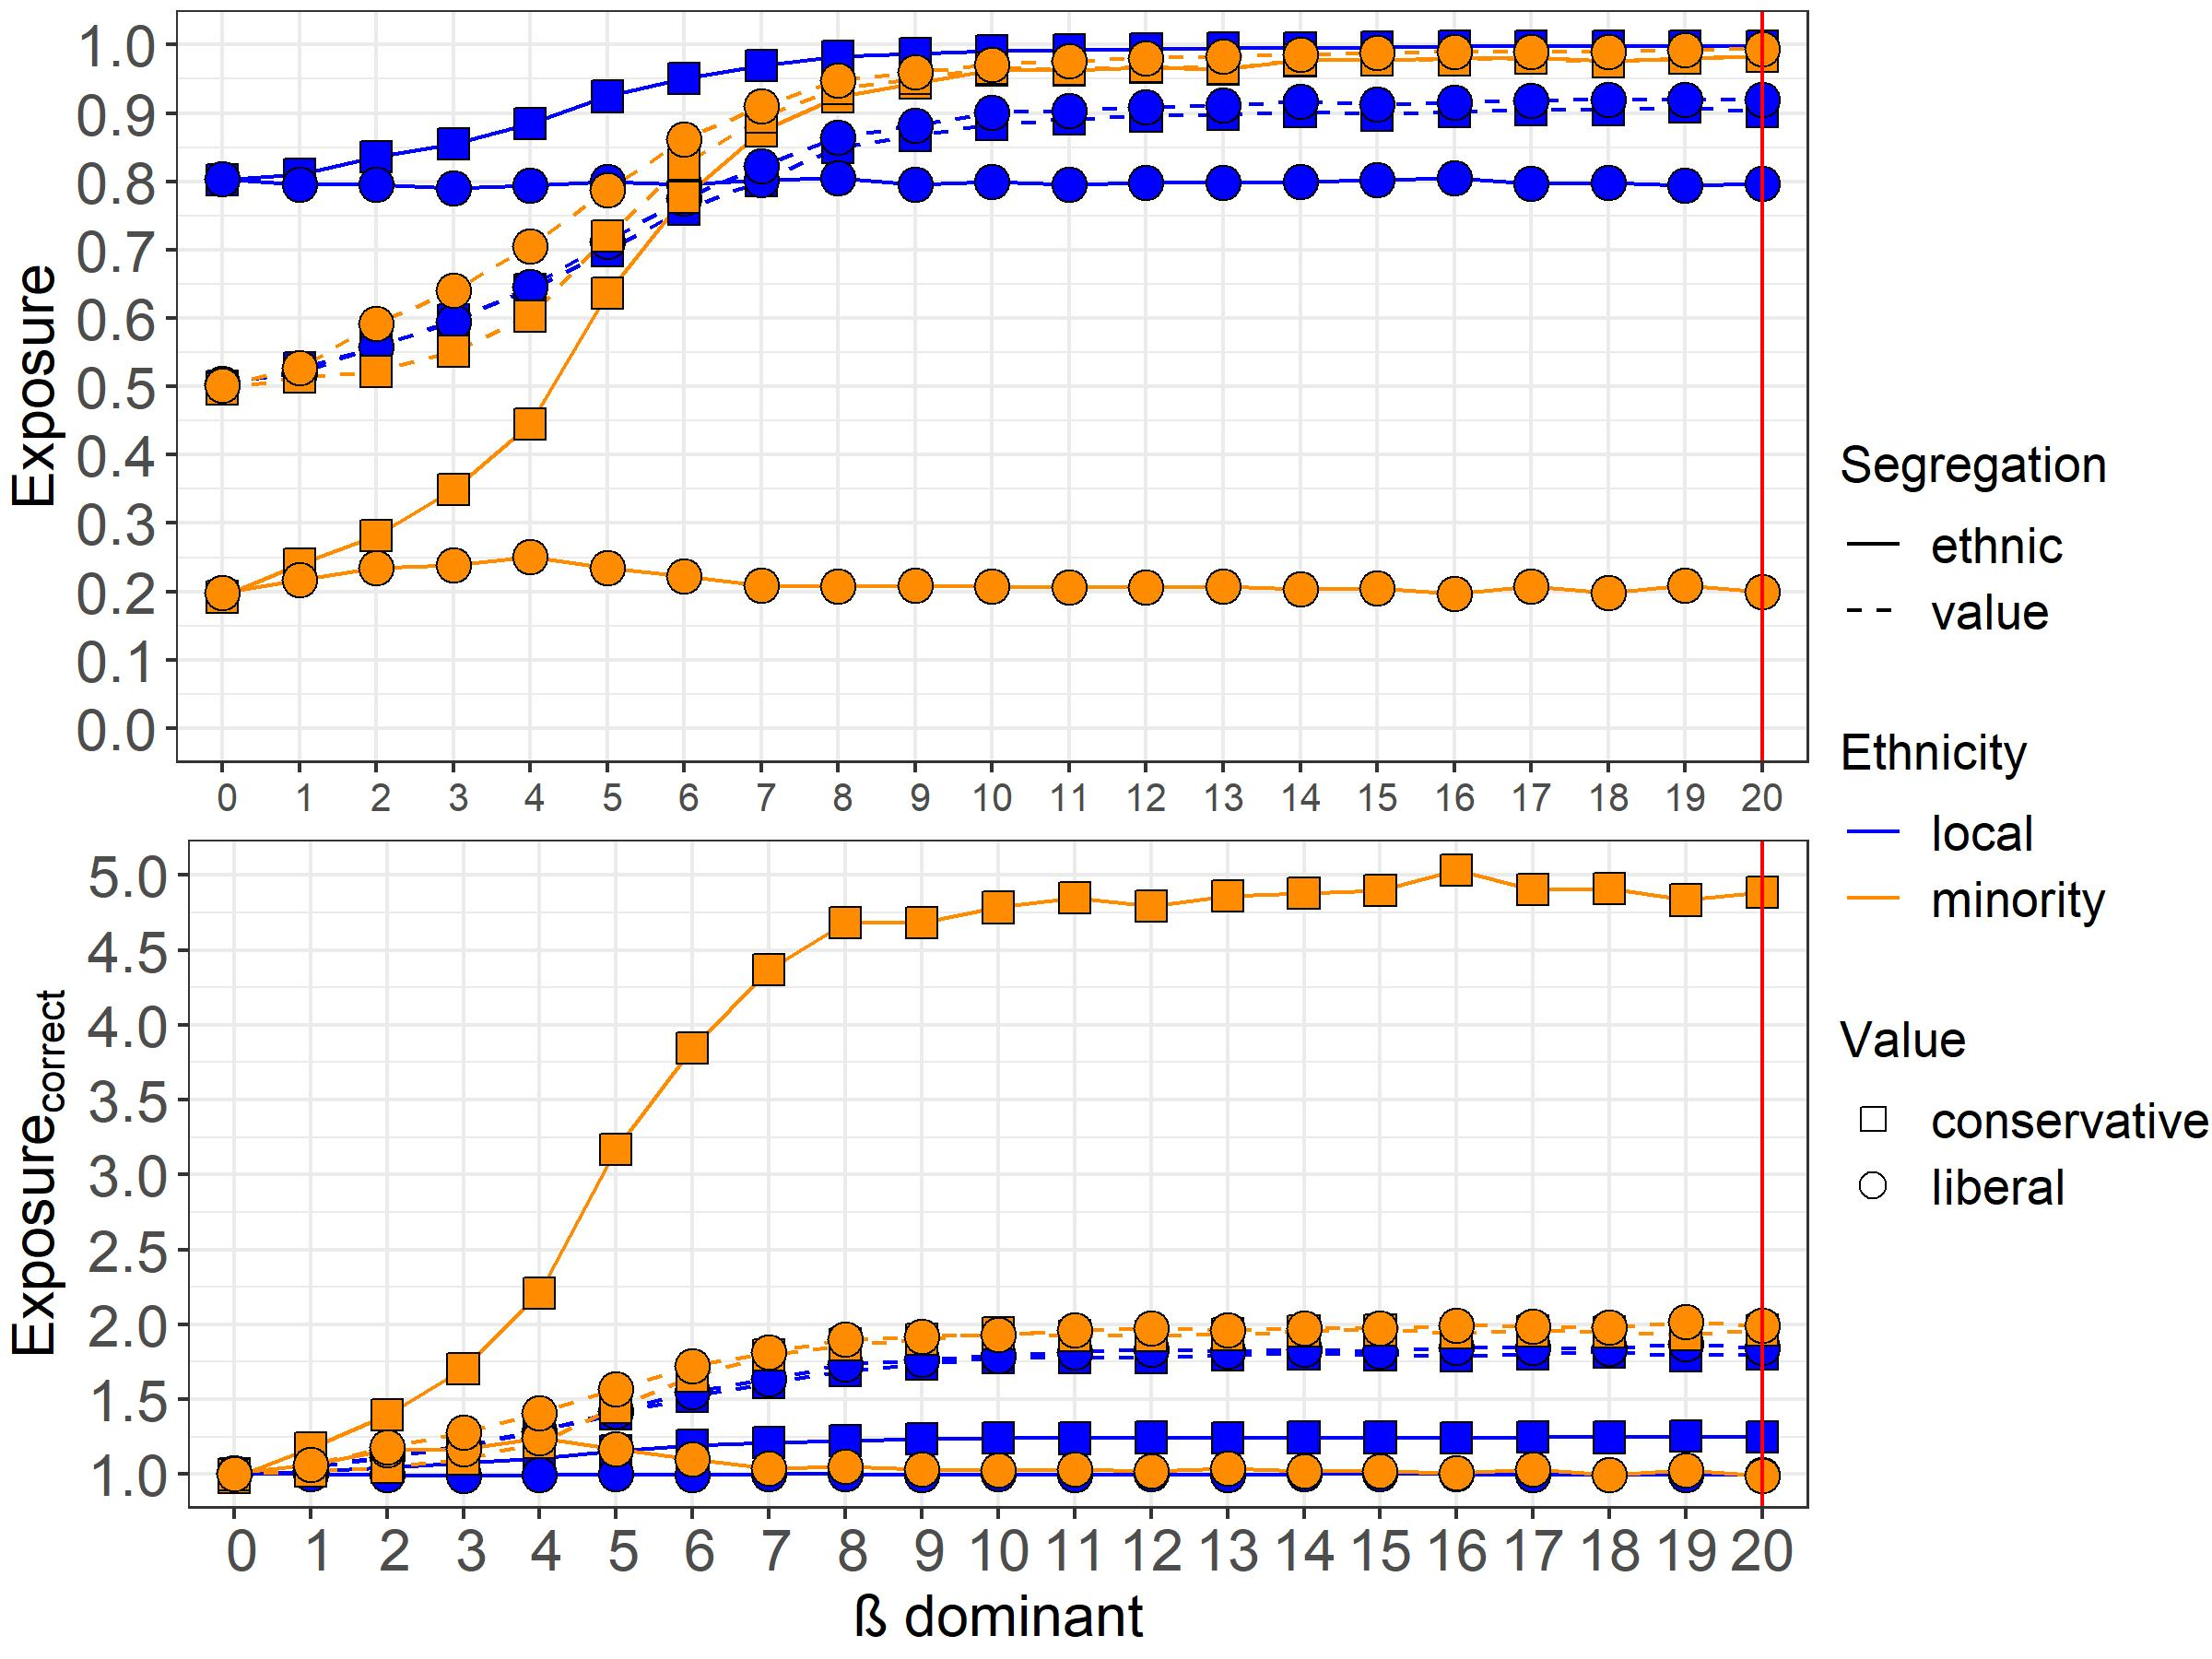
\includegraphics[scale=0.5]{material/figures/asym_dom.jpg}
    \caption{Asymmetric ethnic condition for fig: \ref{fig:sec_0}. $80 \%$ ethnic local, $20 \%$ ethnic minority. In both ethnic groups $50 \%$ liberal agents. Secondary preference =  0}
    \label{fig:asym}
\end{figure} % asymmetric baseline

We run a one-factor-at-time (OFAT) sensitivity analysis \autocite{broeke2016sensitivity} to investigate how each group-type preference differently contributes to stable equilibria in Fig: \ref{fig:asym}. We consider the scenario at $\beta \, dominant = 20$ as nominal set of reference to reproduce. Fig: \ref{fig:sa_asym} compares sensitivity analysis to the dominant preferences of each group-type. For each figure, determinism in preference of each group-type ranges from $\beta = 0$ (total randomness) to $\beta = 20$, while other agents hold $\beta \, dominant = 20$. So, $\beta = 20$ in each graphs reproduces the nominal set in Fig: \ref{fig:asym}. This strategy best serves to observe how decrease of randomness in the relocation choice of each group-type interacts with segregation patterns of other groups to reproduce the final configuration. Neither we have reasons to expect changes in segregation patterns due to parameter range above $\beta = 20$. 

\begin{figure}[H]
    \centering
    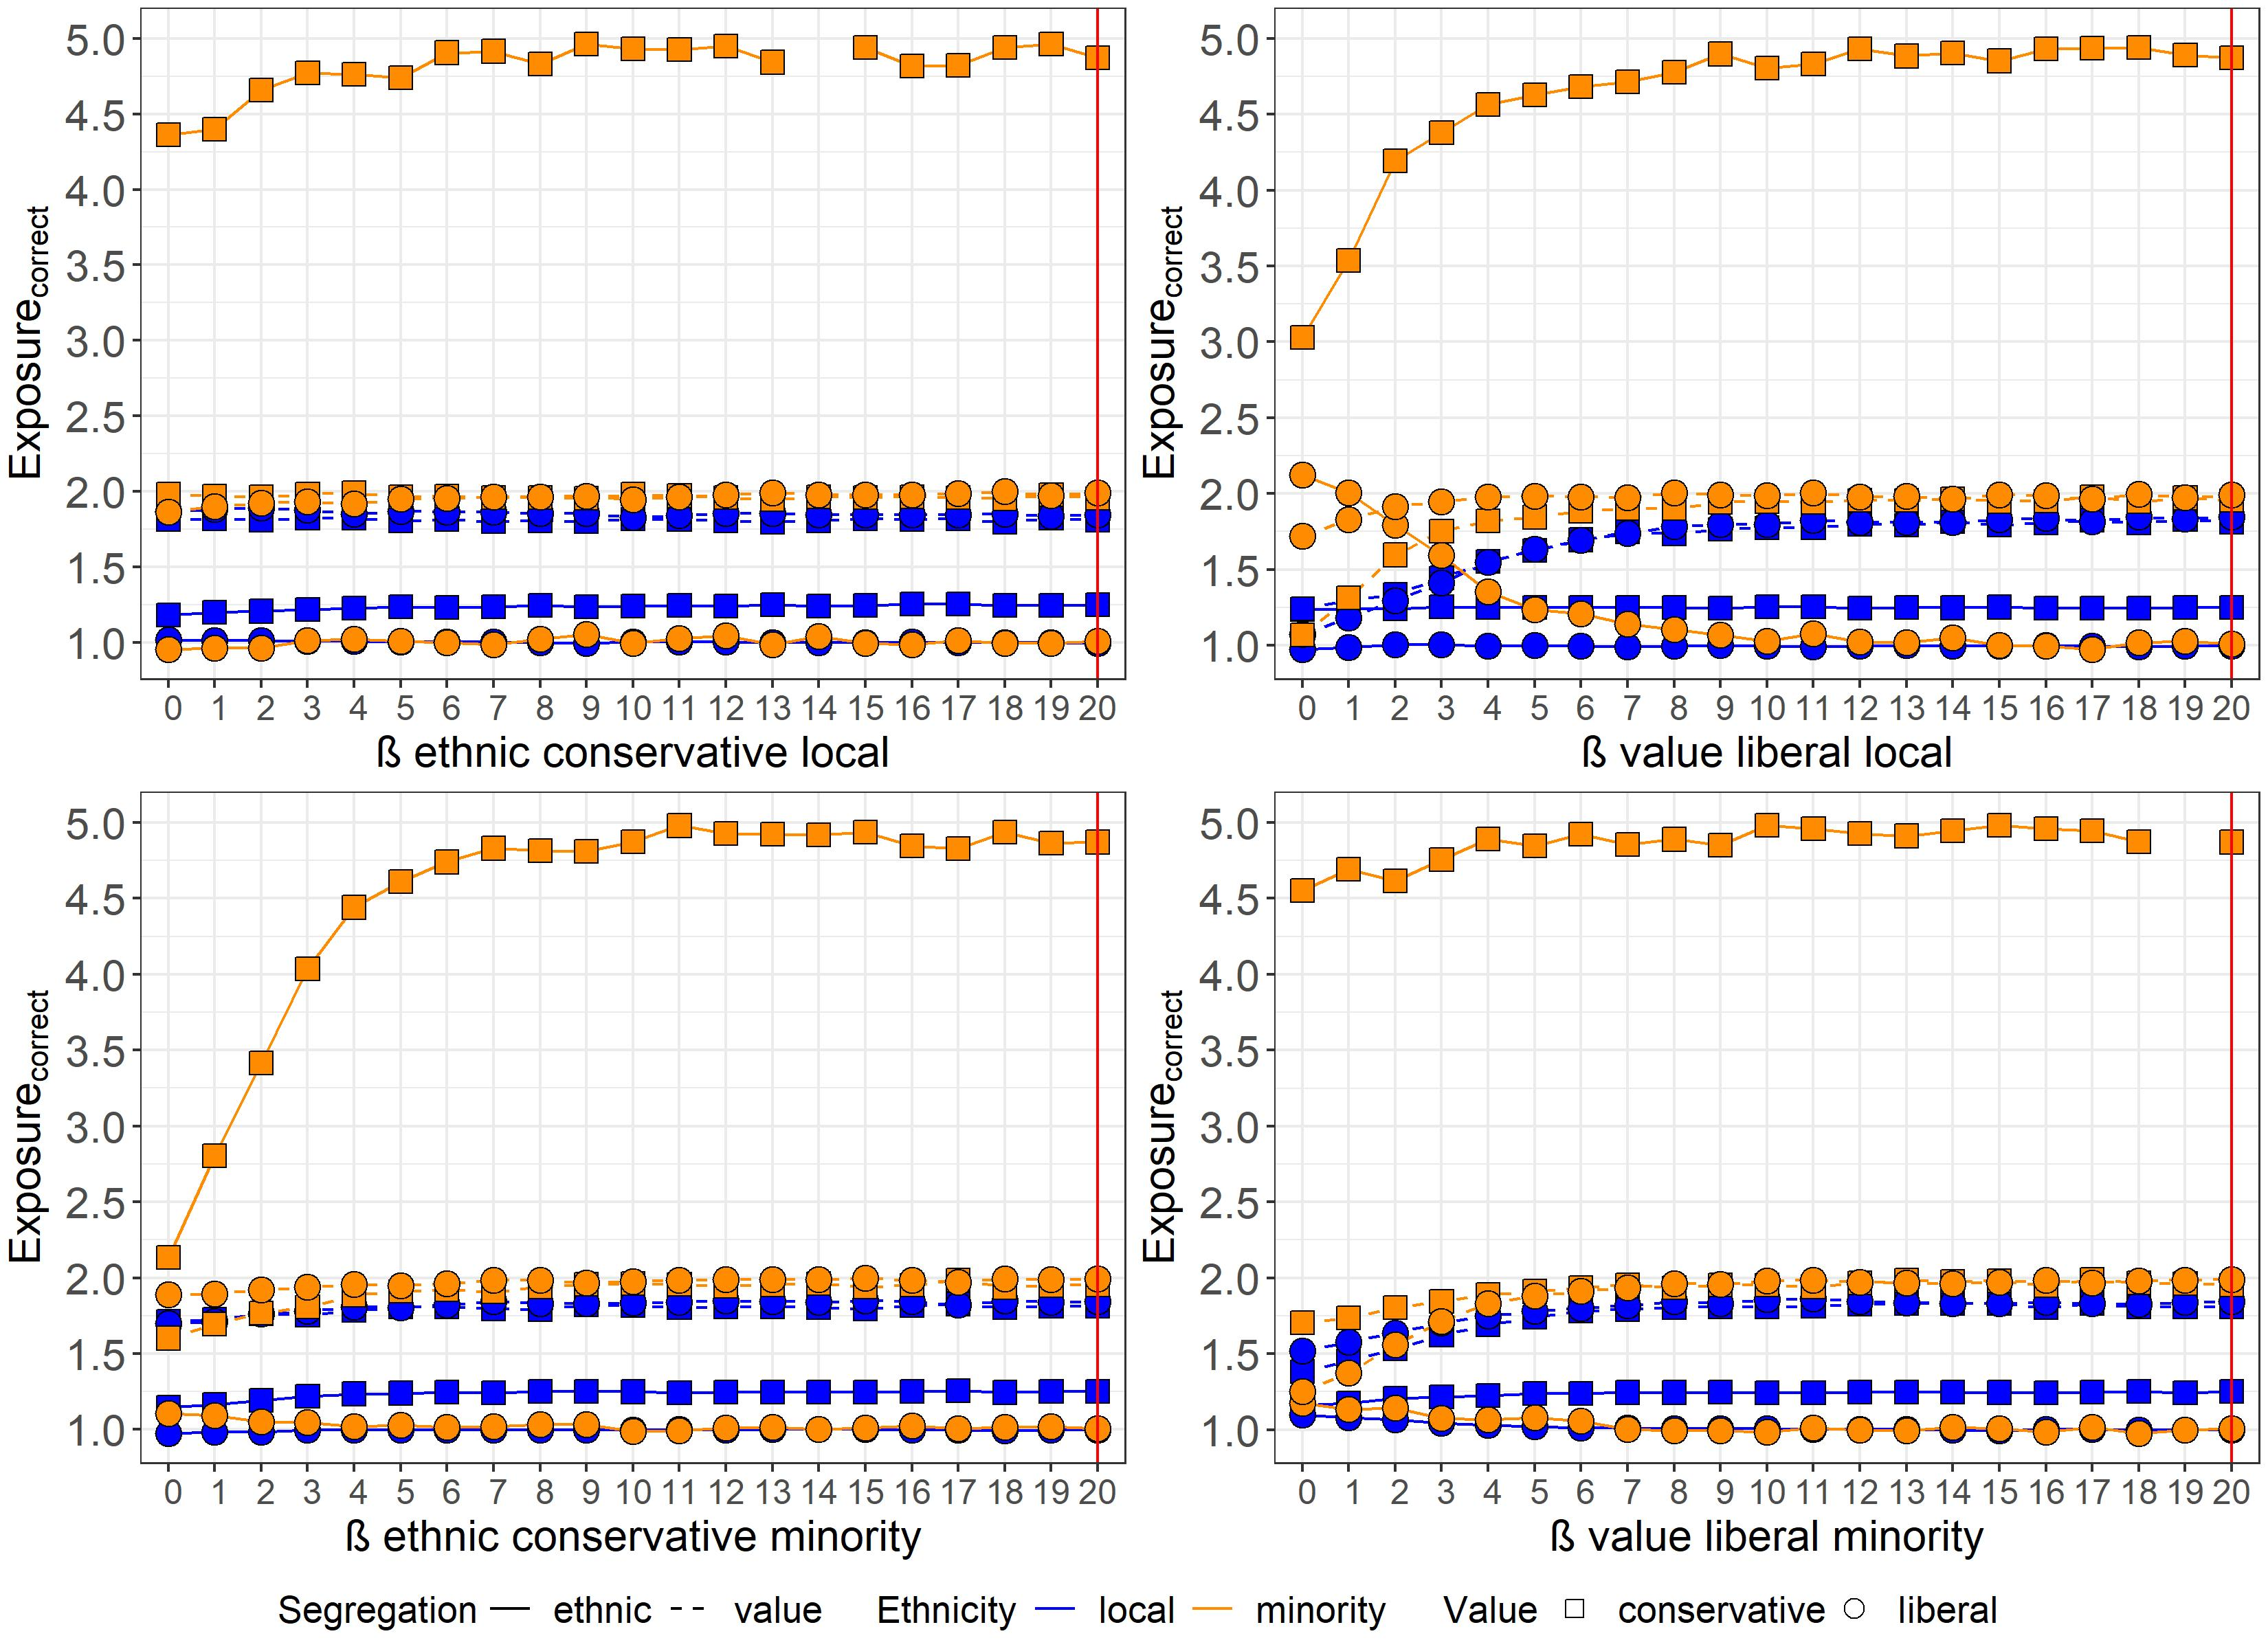
\includegraphics[scale=0.5]{material/figures/sa_asym_bt.jpg}
    \caption{Sensitivity analysis to dominant preference of each group-type for Fig: \ref{fig:asym}. In red the nominal set. For each panel, dominant preference of other agents is $\beta = 20$ \rocco{if looks too rich, since more changes occur for higher randomness, we could report on x-axis only 0-10,then 19-20 as final states}}
    \label{fig:sa_asym}
\end{figure} % asymmetric baseline
%%

Sensitivity to ethnic preference of conservatives majority (top left panel) shows basically no change from the nominal set, which means they do not have a strong influence once other agents hold to their dominant preference. Due to numerical superiority, conservatives majority have less need to cluster to maximize their preference, and high segregation is stable even for low determinism $\beta$. For $\beta \geq 7$, conservatives majority seem to have a reinforce effect on the spatial clustering of conservatives minority.

Top right panel shows sensitivity to value preference of liberals majority, showing how change in their preference affects more substantially the emerging results. As expected, though liberals majority reach full value segregation, they do not spatially segregate for the ethnic dimension ($E^c_i \simeq 1$), still maintaining high ethnic neighborhood exposure. Value segregation of conservatives majority as by-product of value preference of liberals majority is evident, while there is no effect on their ethnic segregation. Major changes occur for the ethnic minority in areas of value liberals majority $\beta \leq 9$ after which stability is reached. Liberals minority show higher ethnic clustering with $E^c_i = 2.125$ (neighborhood exposure $E_i \simeq 0.4$) for $\beta$ liberals majority = 0, declining to the initial random distribution $E^c_i = 1.008$ (neighborhood exposure $E_i \simeq 0.2$) for liberals majority $\beta \geq 9$. This happens because while liberals majority relocate randomly, liberals minority can only count on co-values of their ethnic group to maximize the value utility, so that ethnic segregation increases even if they do not care about ethnicity. Nevertheless, the numerical inferiority does not allow for high ethnic segregation. 
%Liberals majority reinforce value segregation of liberals minority due to their own preference.
% Value segregation of liberals minority increases rapidly from $V^c_i = 1.721$ for $\beta$ liberal local = 0 to $V^c_i = 2$ for $\beta \simeq 3$, showing a reinforce of liberals majority over self-clustering of liberals minority for value similarity. %
Ethnic segregation of conservatives minority increases from $E^c_i = 3.030$ for $\beta$ liberals majority = 0 to $E^c_i \simeq 4.378$ for $\beta = 3$, to then slowly stabilize with $E^c_i \simeq 5$, equal to full ethnic neighborhood exposure. While liberals cluster by value, they limit the space to relocate to conservatives of both groups. However, results reflect how conservatives minority have higher need to cluster to satisfy ethnic preference compared to conservatives majority due to their numerical under-representation. 
% Comparison with increase of value preference liberals minority (bottom right panel) shows how liberals majority have higher effect on behavior of conservatives minority
For value preference of liberals majority $\beta = 0$, value segregation of conservatives minority does not occur ($V^c_i = 1.066$): though liberals minority hold high value preference $\beta = 20$, they are too few to enact the by-product value segregation of conservative agents. As soon as also relocations of liberals majority become more deterministic for value similarity, value segregation of conservatives minority increases to full value segregation $V^c_i \simeq 1.95$ for value liberals majority $\beta \geq 9$. % The trend is similar for value segregation of conservatives majority, though conservatives minority show higher value segregation, due to reinforce of higher ethnic clustering.
% Simultaneously, conservatives minority reach almost full value segregation $V^c_i = 1.955$, i.e. value neighborhood exposure $V_i = 0.977$. for $\beta$ liberals majority = 20.%

Bottom left panel of Fig: \ref{fig:sa_asym} shows increase in ethnic preference of conservatives minority, which only affects their own ethnic segregation showing higher clustering to maximize ethnic utility compared to other group-types. %$E^c_i = 4.871$ for $\beta = 20$.% 
Bottom right panel finally shows changes due to value preference of liberals minority. The comparison with value preference of liberals majority shows how the latter can influence more the system behavior due to ethnic asymmetry, though the mechanisms related to value similarity are the same. Conservatives minority show high levels of both ethnic and value segregation for value liberals minority $\beta <= 7$, because of high value preference of liberals majority in this condition, which is enough to cause by-product value segregation of conservatives minority and reinforce their ethnic self-clustering. Ethnic segregation of liberals minority does not occur due to acceptance by liberals majority which leaves liberals minority in the condition of ethnic assimilation %(insignificant increase occurs for random relocations of liberal minority, peak at $\beta$ liberal minority = 0 with $E^c_i = 1.176$).


\begin{figure}[H]
    \centering
    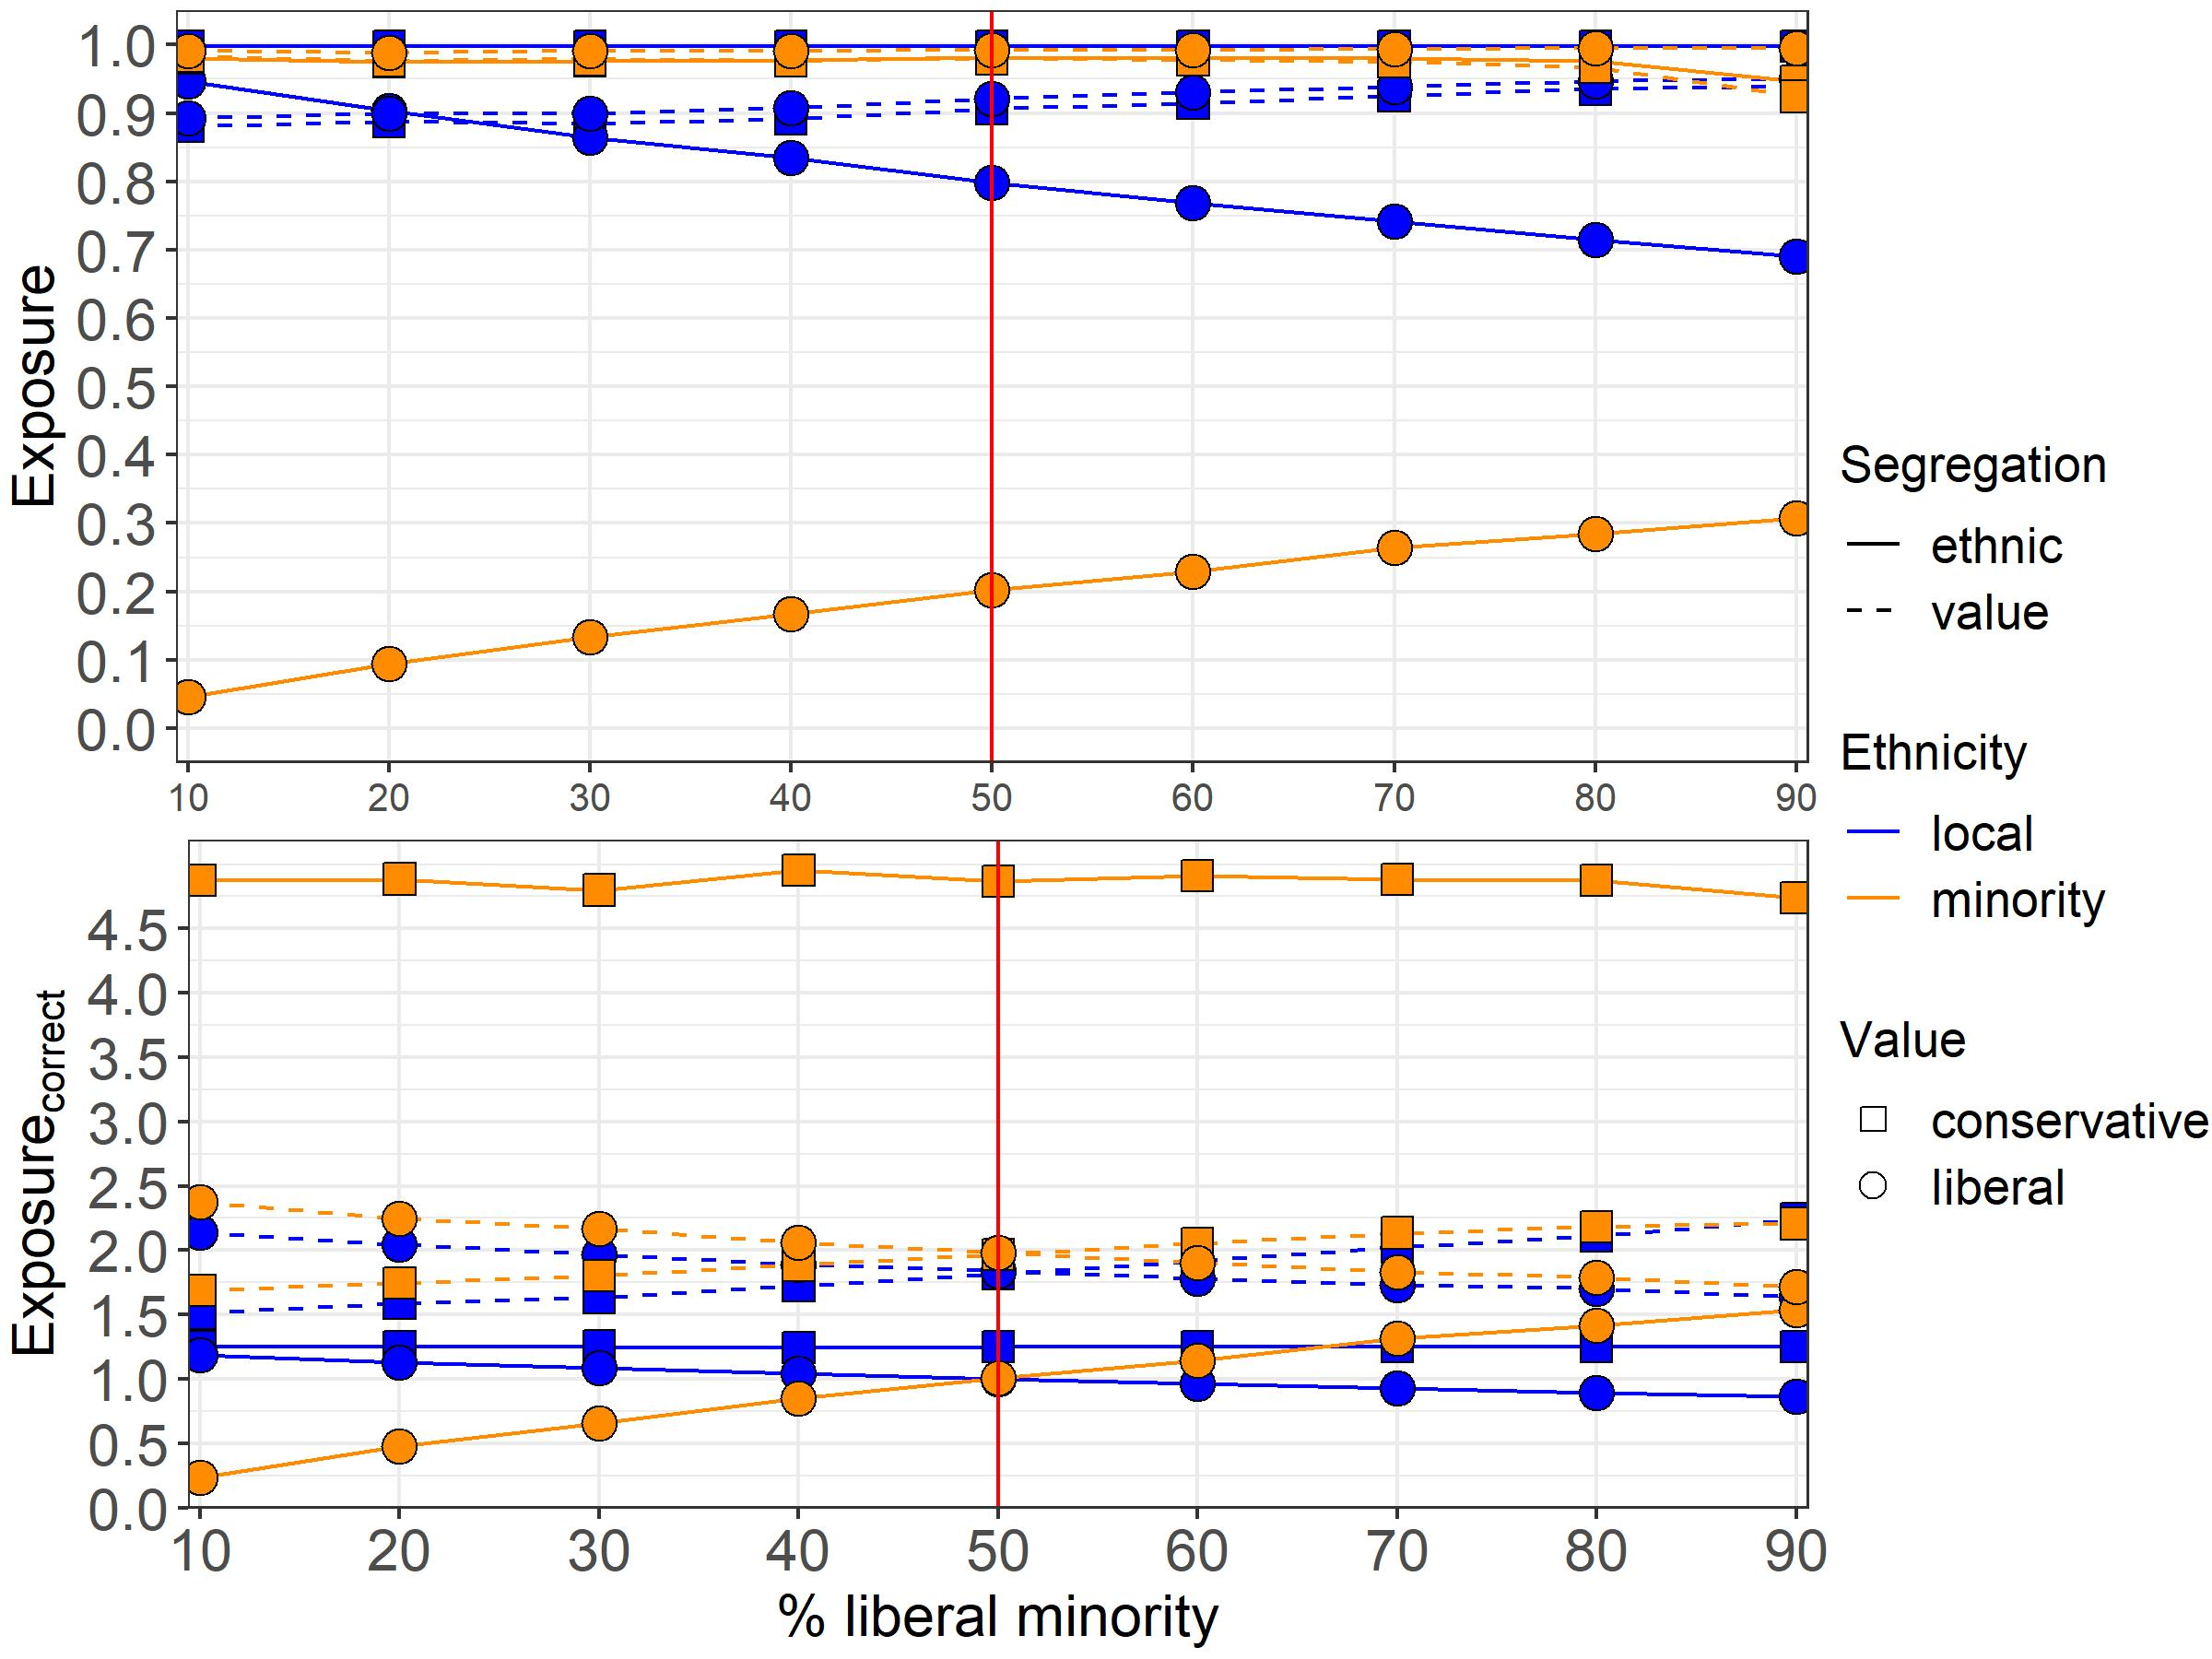
\includegraphics[scale=0.5]{material/figures/comb_dislib.jpg}
    \caption{Sensitivity analysis of Fig: \ref{fig:asym} to distribution of liberals. Red intercept corresponds to nominal set in Fig: \ref{fig:asym}.}
    \label{fig:dislib}
\end{figure} % dislib

In Fig: \ref{fig:dislib} we observe the effect of distribution of liberals in the minority group before exploring how it interacts with preferences of agents. We are interested in this parameter since it directly affects the value utility of neighborhoods for agents of both ethnic groups while ethnic asymmetry remains. On the x-axis, the percentage of liberals minority shifts from a $10 \%$ to $90 \%$, we exclude the conditions with no conservatives minority or no liberals minority since trivial.
In all conditions each group-type holds $\beta \, dominant = 20$, so that the condition of $50 \%$ liberals minority equals to nominal set in Fig: \ref{fig:asym}. Results show a linear effect of distribution of liberals minority on segregation scenarios: ethnic segregation of liberals majority decreases from $E_i = 0.946$ for $10 \%$ to $E_i = 0.691$ for $90 \%$, while ethnic segregation of liberals minority increases from $E_i = 0.046$ for $10 \%$ to $E_i = 0.308$ for $90 \%$. Simply, as the percentage of liberals in the ethnic minority increases, there is eventually more chance for liberals minority to find a co-value among co-ethnics, so as for liberals majority to find a co-value of the other ethnicity, which compensates for ethnic asymmetry. Value exposure remains high for liberals of both groups in all conditions ($V^c_i \simeq 2$, i.e. $0.99 \geq V_i \geq 0.88$), since the percentage of liberals in the whole population increases overall \footnote{See table \ref{tab:dislib_exp} for detailed conditions}.

As for interaction with preferences of each group-type, Fig: \ref{fig:sa_asym} shows how liberals drive more changes into segregation patterns due to mechanisms associated with value similarity, though larger effects are due to liberals in the numerical majority condition. For the sake of shortness, we therefore limit the analysis to the interaction of distribution of liberals minority with value preference of liberals majority and liberals minority. We select conditions of under-representation of liberals minority $20 \%$, and over-representation $80 \%$, compared to the baseline condition of $50 \%$. In each graph, other agents hold dominant preference $\beta = 20$ and secondary preference $\beta = 0$, while liberals of either ethnic group increase their value preference on the x-axis. Panels from top to bottom report the condition of $20 \%$, $50 \%$ and $80 \%$ liberals minority. So, $\beta = 20$ for $50 \%$ liberal minority corresponds to the nominal set in Fig: \ref{fig:asym}.


Fig: \ref{fig:vllblc} focuses on increase of value preference of liberals majority. For value liberals majority $\beta = 20$, value segregation of conservatives majority shifts from $V^c_i = 1.584$, i.e. value neighborhood exposure $V_i = 0.871$ with $20 \%$ liberals minority, to $V^c_ i = 2.199$, i.e. $V_i = 0.953$ with $80 \%$ liberals minority. That is, the by-product value segregation of conservatives increases because the percentage of liberals increases in the whole population. No changes occur for ethnic segregation of conservatives majority.
Due to higher chance to find a co-value in the minority group, ethnic segregation of liberals majority falls below $E^c_i = 1$ for over-representation of $80 \%$ liberals minority, though high neighborhood ethnic exposure remains. Conversely, liberals minority driven by value similarity show a tendency towards spatial ethnic segregation when liberals majority relocate randomly for  $\beta \leq 5$. The peak is reached for liberals majority $\beta = 0$ and $80 \%$ liberals minority, where liberals minority reach $E^c_i = 2.5$, i.e. ethnic exposure $E_i = 0.5$. Nevertheless, this integration outcome occurs because liberals minority are not enough to form full segregated neighborhoods. In the $80 \%$  condition, liberals minority show spatial ethnic segregation also for higher value preference of liberals majority ($E^c_i \simeq 1,4$), though remaining ethnically assimilated to them ($E_i = 0.28$). For conservatives minority, differences due to distribution of liberals minority are more evident in the region of random relocations of liberals majority. For value liberals majority $\beta = 0$, ethnic segregation of conservatives minority decreases from $E^c_i = 3.030$, i.e. neighborhood ethnic exposure $E_i = 0.606$ with $50 \%$ liberals minority to $E^c_i = 2.243$, i.e. ethnic assimilation $E_i = 0.44$ for the $80 \%$ condition. Also value segregation of conservatives minority decreases, from $V^c_i = 1.066$, i.e. neighborhood value integration $V_i = 0.533$ in the baseline condition, to value assimilation $V^c_i = 0.562$, i.e. $V_i = 0.2529$ for $80 \%$ liberal minority. Although the number of liberals in the population increases, in this condition liberals majority relocate randomly and only liberals minority hold high value preference. However, they are not numerically enough to cause by-product value segregation of conservatives or reinforce their clustering reducing areas of relocation. As soon as also liberals majority increase their preference, the two mechanisms are enacted, with increase to almost complete value and ethnic segregation. For $20 \%$ liberals minority, these results do not occur: almost all ethnic minority is conservative, so to form a critical mass to reach high ethnic segregation and not being affected by preferences of other agents. High value segregation occurs because of clustering with co-ethnics who are also co-values, so to not show differences when liberals majority increase value preference. 

Fig: \ref{fig:vllbmn} shows the increase in value preferences of liberals minority while other agents, including liberals majority, hold dominant $\beta = 20$. Differences with Fig: \ref{fig:vllblc} are more evident for conservatives minority and liberals minority in the regions of higher randomness. Conservatives minority show high ethnic and value segregation for random relocations of liberals minority because of high value preference of liberals majority $\beta = 20$, which is enough to enact by-product value segregation and reinforce of ethnic clustering. Difference due to increase in value preference of liberals minority is low. Ethnic segregation of liberals minority as effect of their clustering by value similarity does not occur, because they are already accepted by liberals majority. For $20 \%$ liberals minority distribution, the process leads to even further ethnic assimilation to liberals majority. When the percentage of liberals minority raises to $80 \%$ instead, there is higher chance for liberals minority to find a co-value in the own group, so to increase ethnic segregation as by-product of the own value preference, though remaining under-represented, with $E_i = 0.30$.
\rocco{To shorten and for content of results, figures \ref{fig:vllblc} and \ref{fig:vllbmn} might be combined. Also, to better understand results described on how liberals majority/minority influence each other, would be good to have a condition with other-group preference = 0, but this increases complexity of the pictures. Will think about}

\begin{figure}[H]
    \centering
    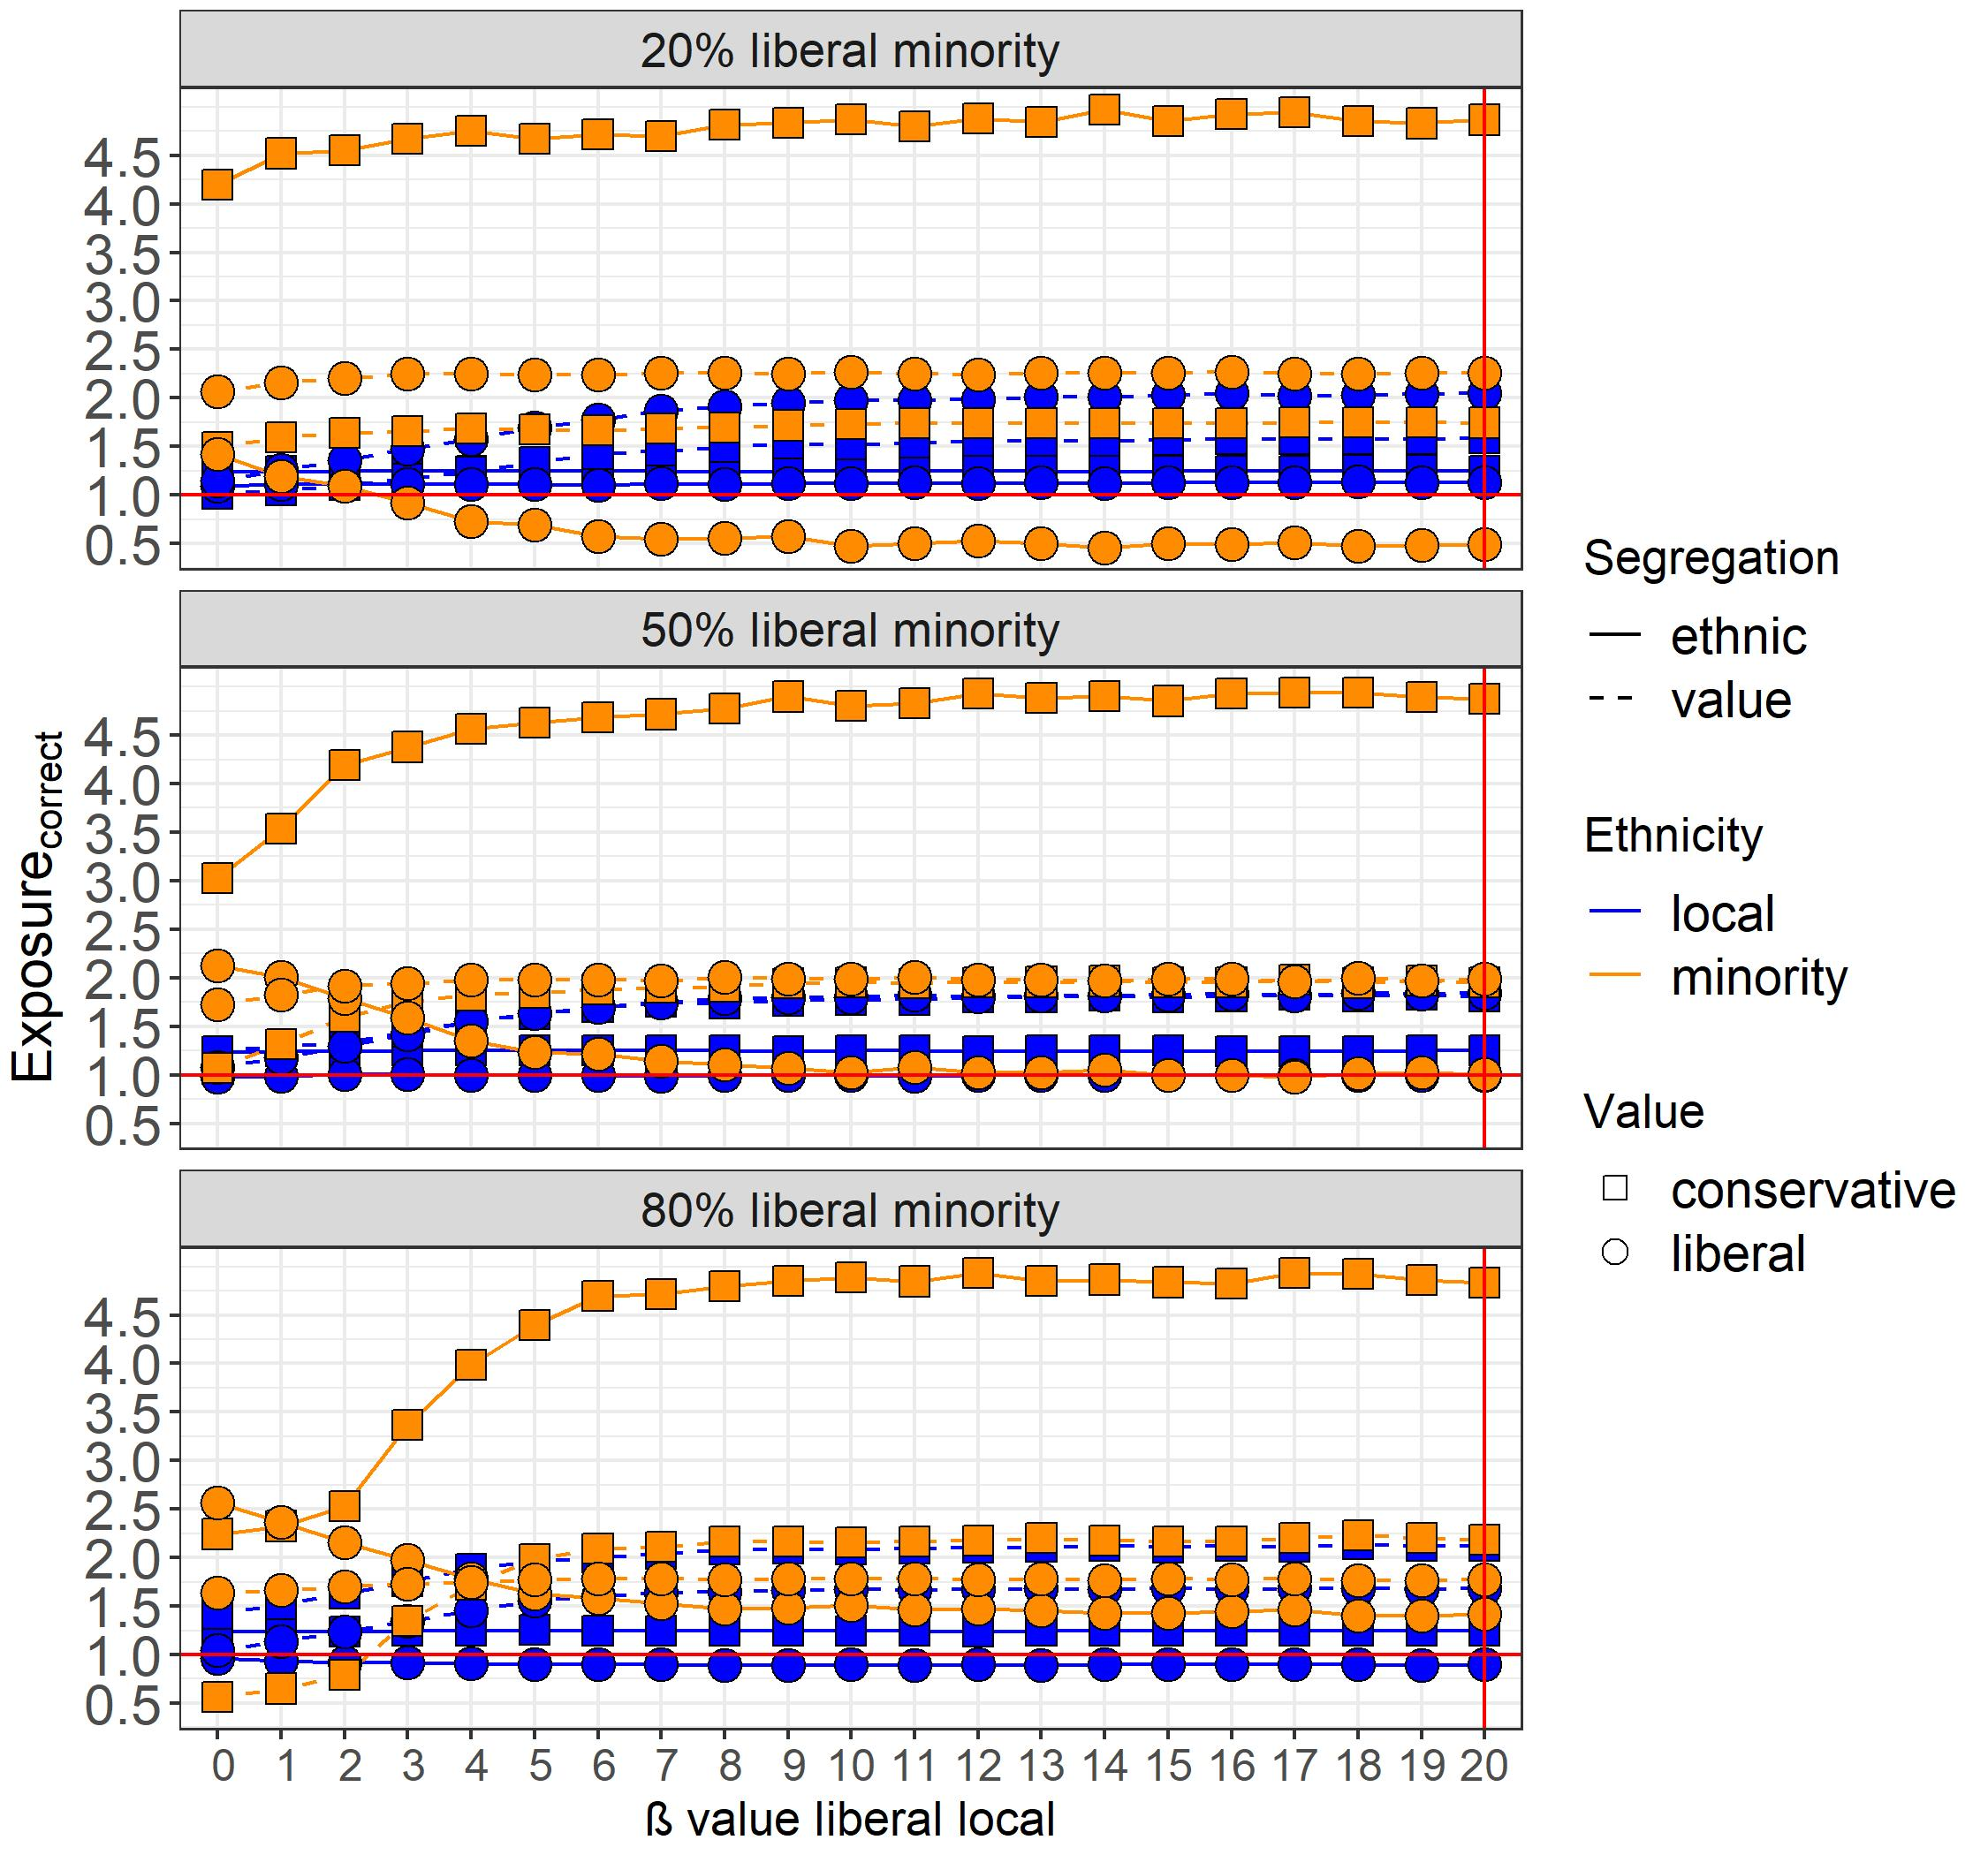
\includegraphics[scale=0.5]{material/figures/vllblc.jpg}
    \caption{Sensitivity analysis of fig: \ref{fig:asym} to interaction of value preference of liberal locals and distribution of liberal minority \rocco{to blend with Fig: \ref{fig:vllbmn}? now text treat differently}}
    \label{fig:vllblc}
\end{figure} % vllblc*min


\begin{figure}[H]
    \centering
    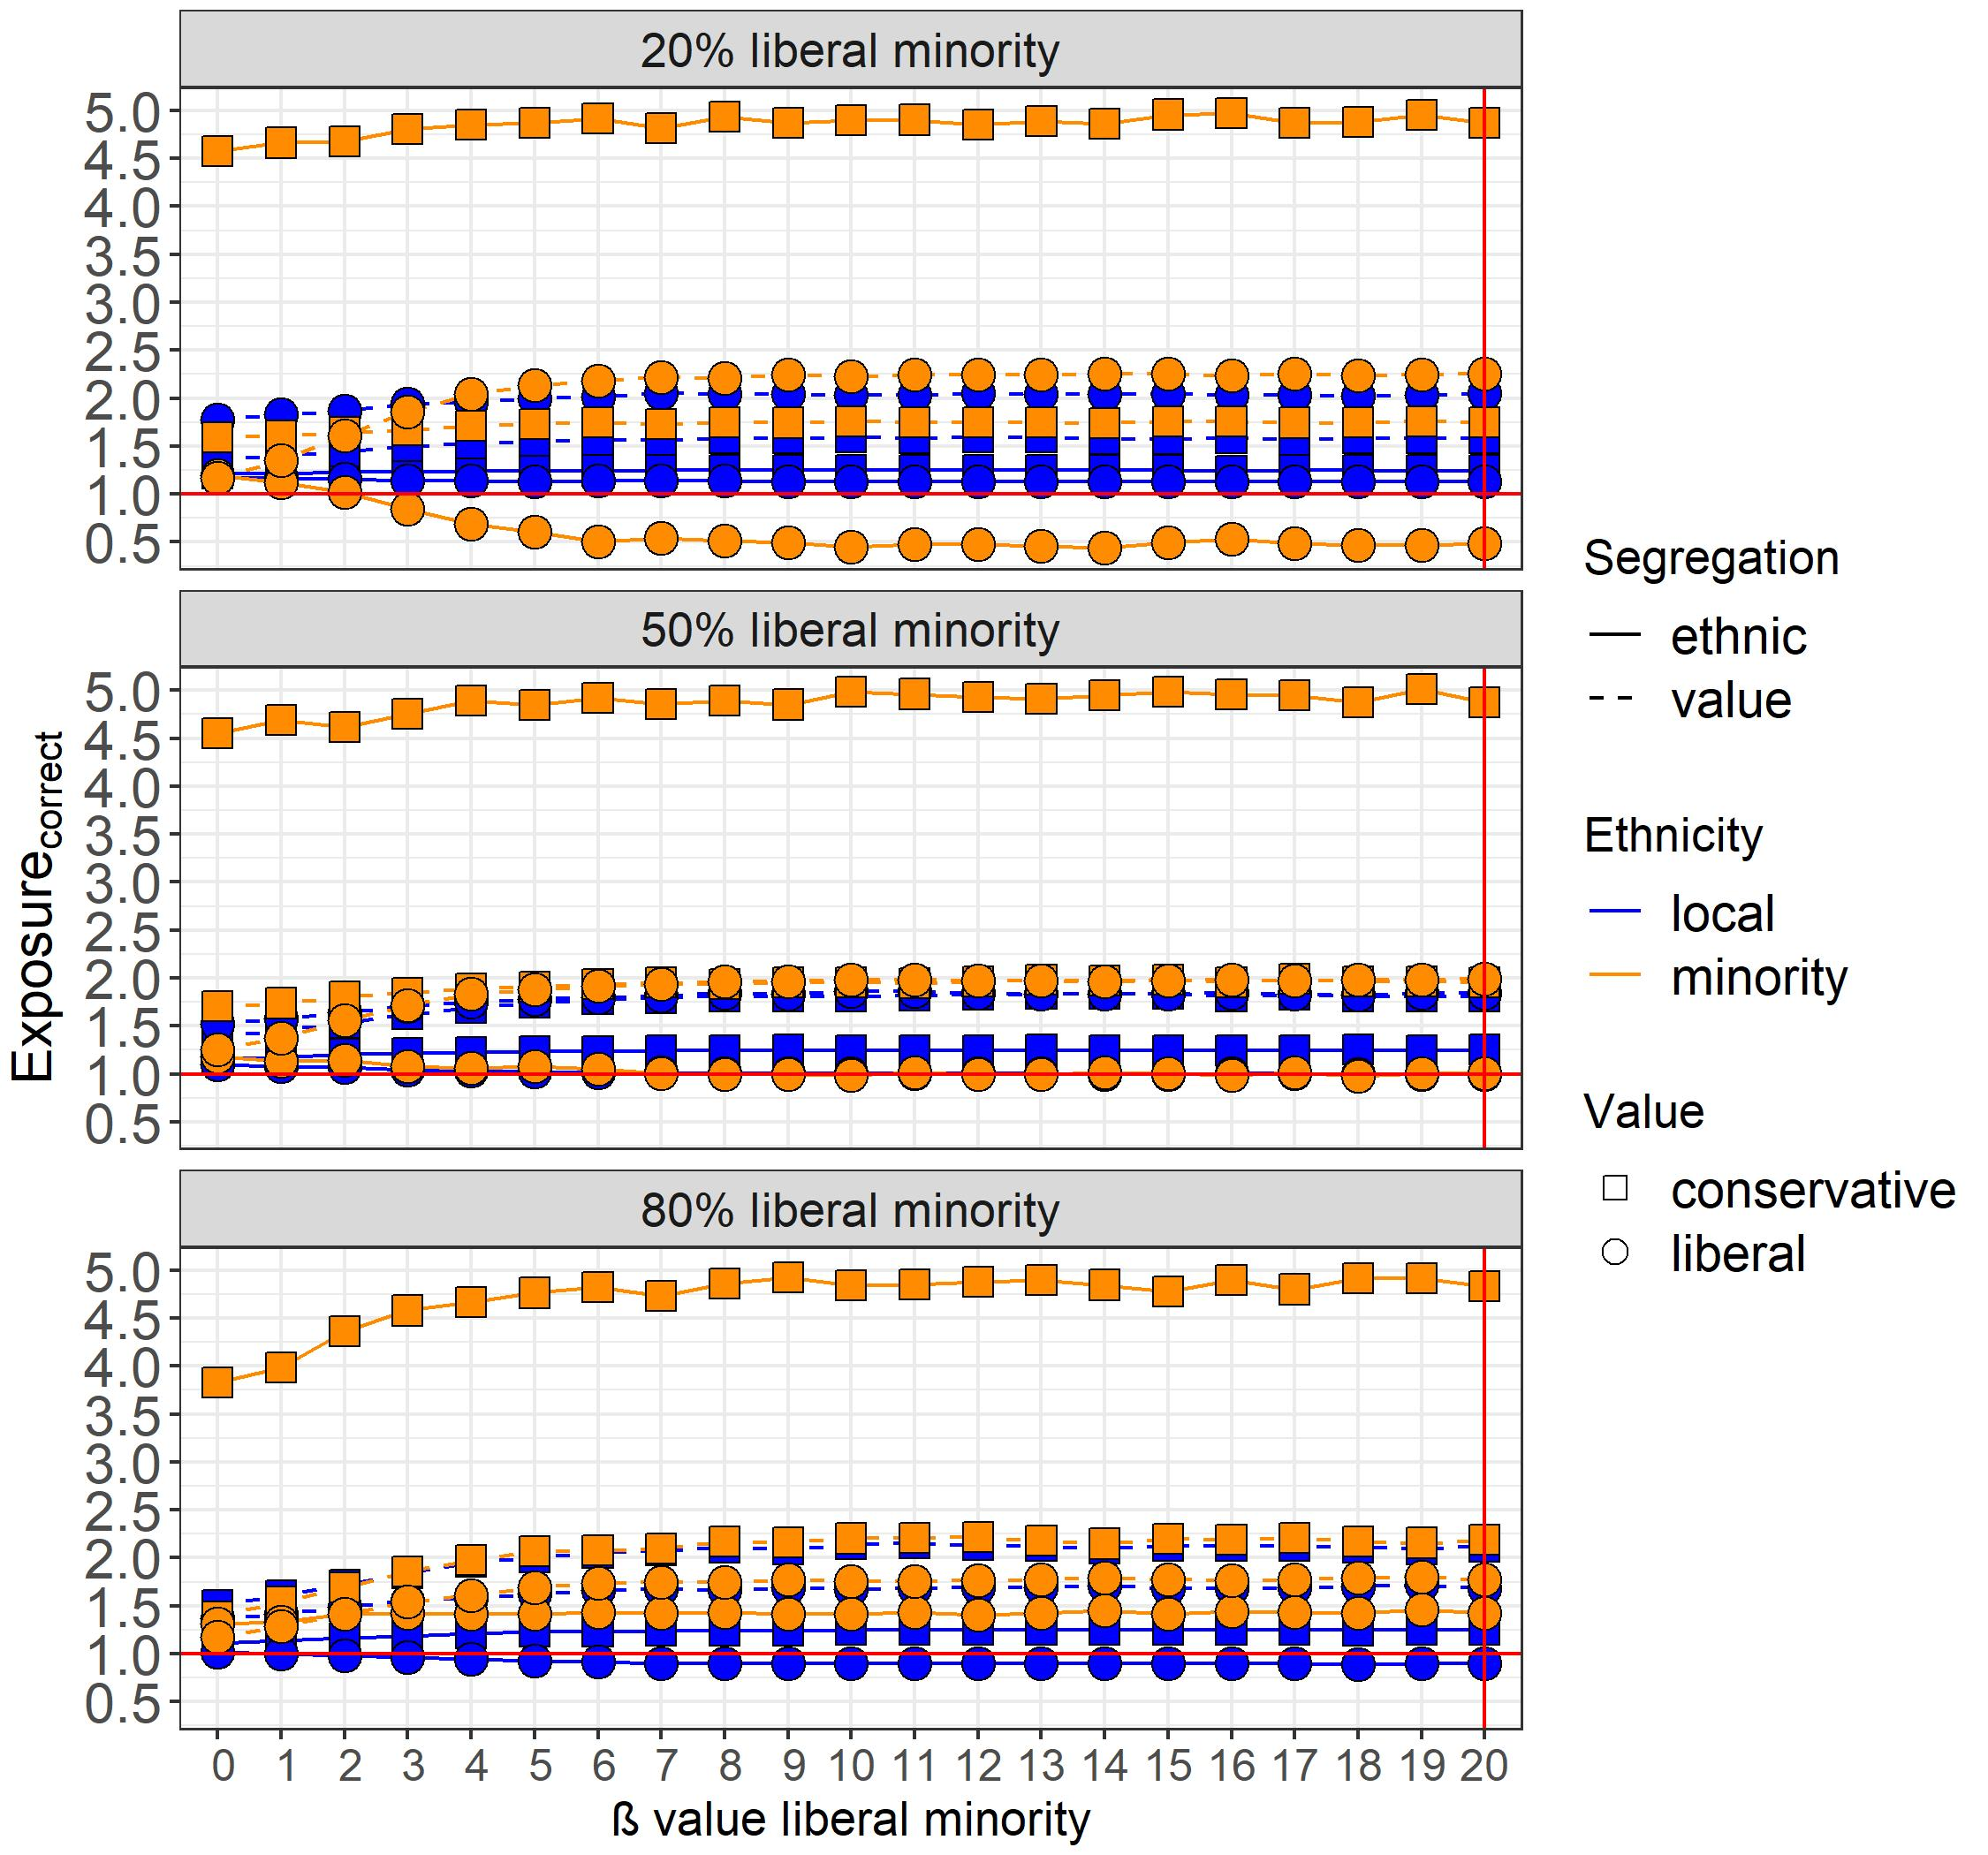
\includegraphics[scale=0.5]{material/figures/vllbmn.jpg}
    \caption{Sensitivity analysis of fig: \ref{fig:asym} to interaction of value preference of liberal minority and distribution of liberal minority \rocco{to blend with Fig: \ref{fig:vllblc}? now text treat differently}}
    \label{fig:vllbmn}
\end{figure} % vllbmn*min

In the last paragraph we test how effects due to value similarity would differ if liberals majority or liberals minority take into consideration also ethnic preferences, and how results would vary for different distribution of liberals minority. This is also a plausible scenario, meaning people prefer to live close to others who share particular characteristics (e.g. similar ses, political views  etc.) but still would prefer to live with co-ethnics who share such characteristics than out-groups. In each figure, all agents hold their dominant preference $\beta = 20$ and secondary $\beta = 0$, while liberals increase their ethnic preference on the x-axis. This means that within each ethnic group, liberals are still more tolerant than conservatives co-ethnics, holding lower ethnic preference. $\beta = 20$ equals to an ethnic group holding homogeneous high ethnic preference against out-groups.% The condition of ethnic preference $\beta = 0$ in $50 \%$ liberals minority thus equals to the nominal set in baseline Fig: \ref{fig:asym}.

Fig: \ref{fig:et_libloc} reports increase in ethnic preference of liberals majority. Changes in spatial ethnic segregation of the majority population are not evident, due to over-representation. The most evident result is the increase in ethnic segregation of liberals minority who do not care about ethnic preference. While liberals majority would accept liberals minority because of value similarity, they would prefer a co-value of the same ethnic group, forming neighborhoods both ethnic and value homogeneous. As a consequence, liberals minority also form neighborhoods both value and ethnic homogeneous, though as by-product of preference of liberals majority, relocating at the periphery of the neighborhoods liberals majority form (see Fig: \ref{fig:80_etlib}). For ethnic liberals majority $\beta = 20$, and $50 \%$ liberals minority, the by-product tendency towards segregation brings to ethnic integration, with $E^c_i = 2.650$, i.e. $E_i = 0.53$. With increase in the percentage of liberals minority to $80 \%$, their ethnic segregation increases to $E^c_i = 3.355$, equal to neighborhood exposure $E_i = 0.67$. Moreover, for $80 \%$ liberals minority, value segregation of conservatives minority decreases with increase of ethnic preference of liberals majority: from $V^c_i = 2.209$ equal to full neighborhood exposure $V_i = 0.99$ for ethnic liberals majority $\beta = 0$ to $V^c_i =1.583$, i.e. $V_i = 0.71$, for ethnic liberals majority $\beta = 20$. While value segregation decreases, ethnic segregation of conservatives minority remain stable and high. This occurs because, as described earlier, liberals minority concentrate on the edge of larger neighborhoods formed by liberals majority, forming clusters that become ethnically attractive to conservatives minority who are not a threat to their value utility due to their lower numerosity. 

Fig: \ref{fig:et_libmin} replicates for ethnic preferences of liberals minority. The most evident result comparing with Fig: \ref{fig:et_libloc} is that ethnic segregation of liberals minority still occurs, though as effect of their own self-clustering. Liberals minority can not induce ethnic segregation of liberals majority due to ethnic asymmetry. The most noteworthy difference is that value segregation of conservatives minority does not occur when liberals minority increase ethnic preference in the $80 \%$ condition. The difference relies on different spatial relocation of liberals minority (see Fig: \ref{fig:80_etlib}). As in this condition liberals minority want to maximize also ethnic preference, they have higher need to cluster with co-ethnics due to numerical inferiority. Though they would accept also conservatives co-ethnics in this condition, they would still prefer liberals co-ethnic, forming neighborhoods both value and ethnic homogeneous. Because of concentration of liberals, these neighborhoods are attractive also to liberals majority, who are indifferent to their ethnic composition. The final configuration is that of large neighborhoods value homogeneous but internally highly segregated. Liberals minority do not relocate on the edge of such neighborhoods as in Fig: \ref{fig:et_libloc}, but rather form ethnic clusters within the neighborhood. As a matter of fact, the value homogeneity of neighborhoods and their spatial configuration do not let for conservatives minority to be accepted because of value orientation, causing by-product value segregation and reinforce of ethnic segregation as in the baseline condition. 


\begin{figure}[H]
    \centering
    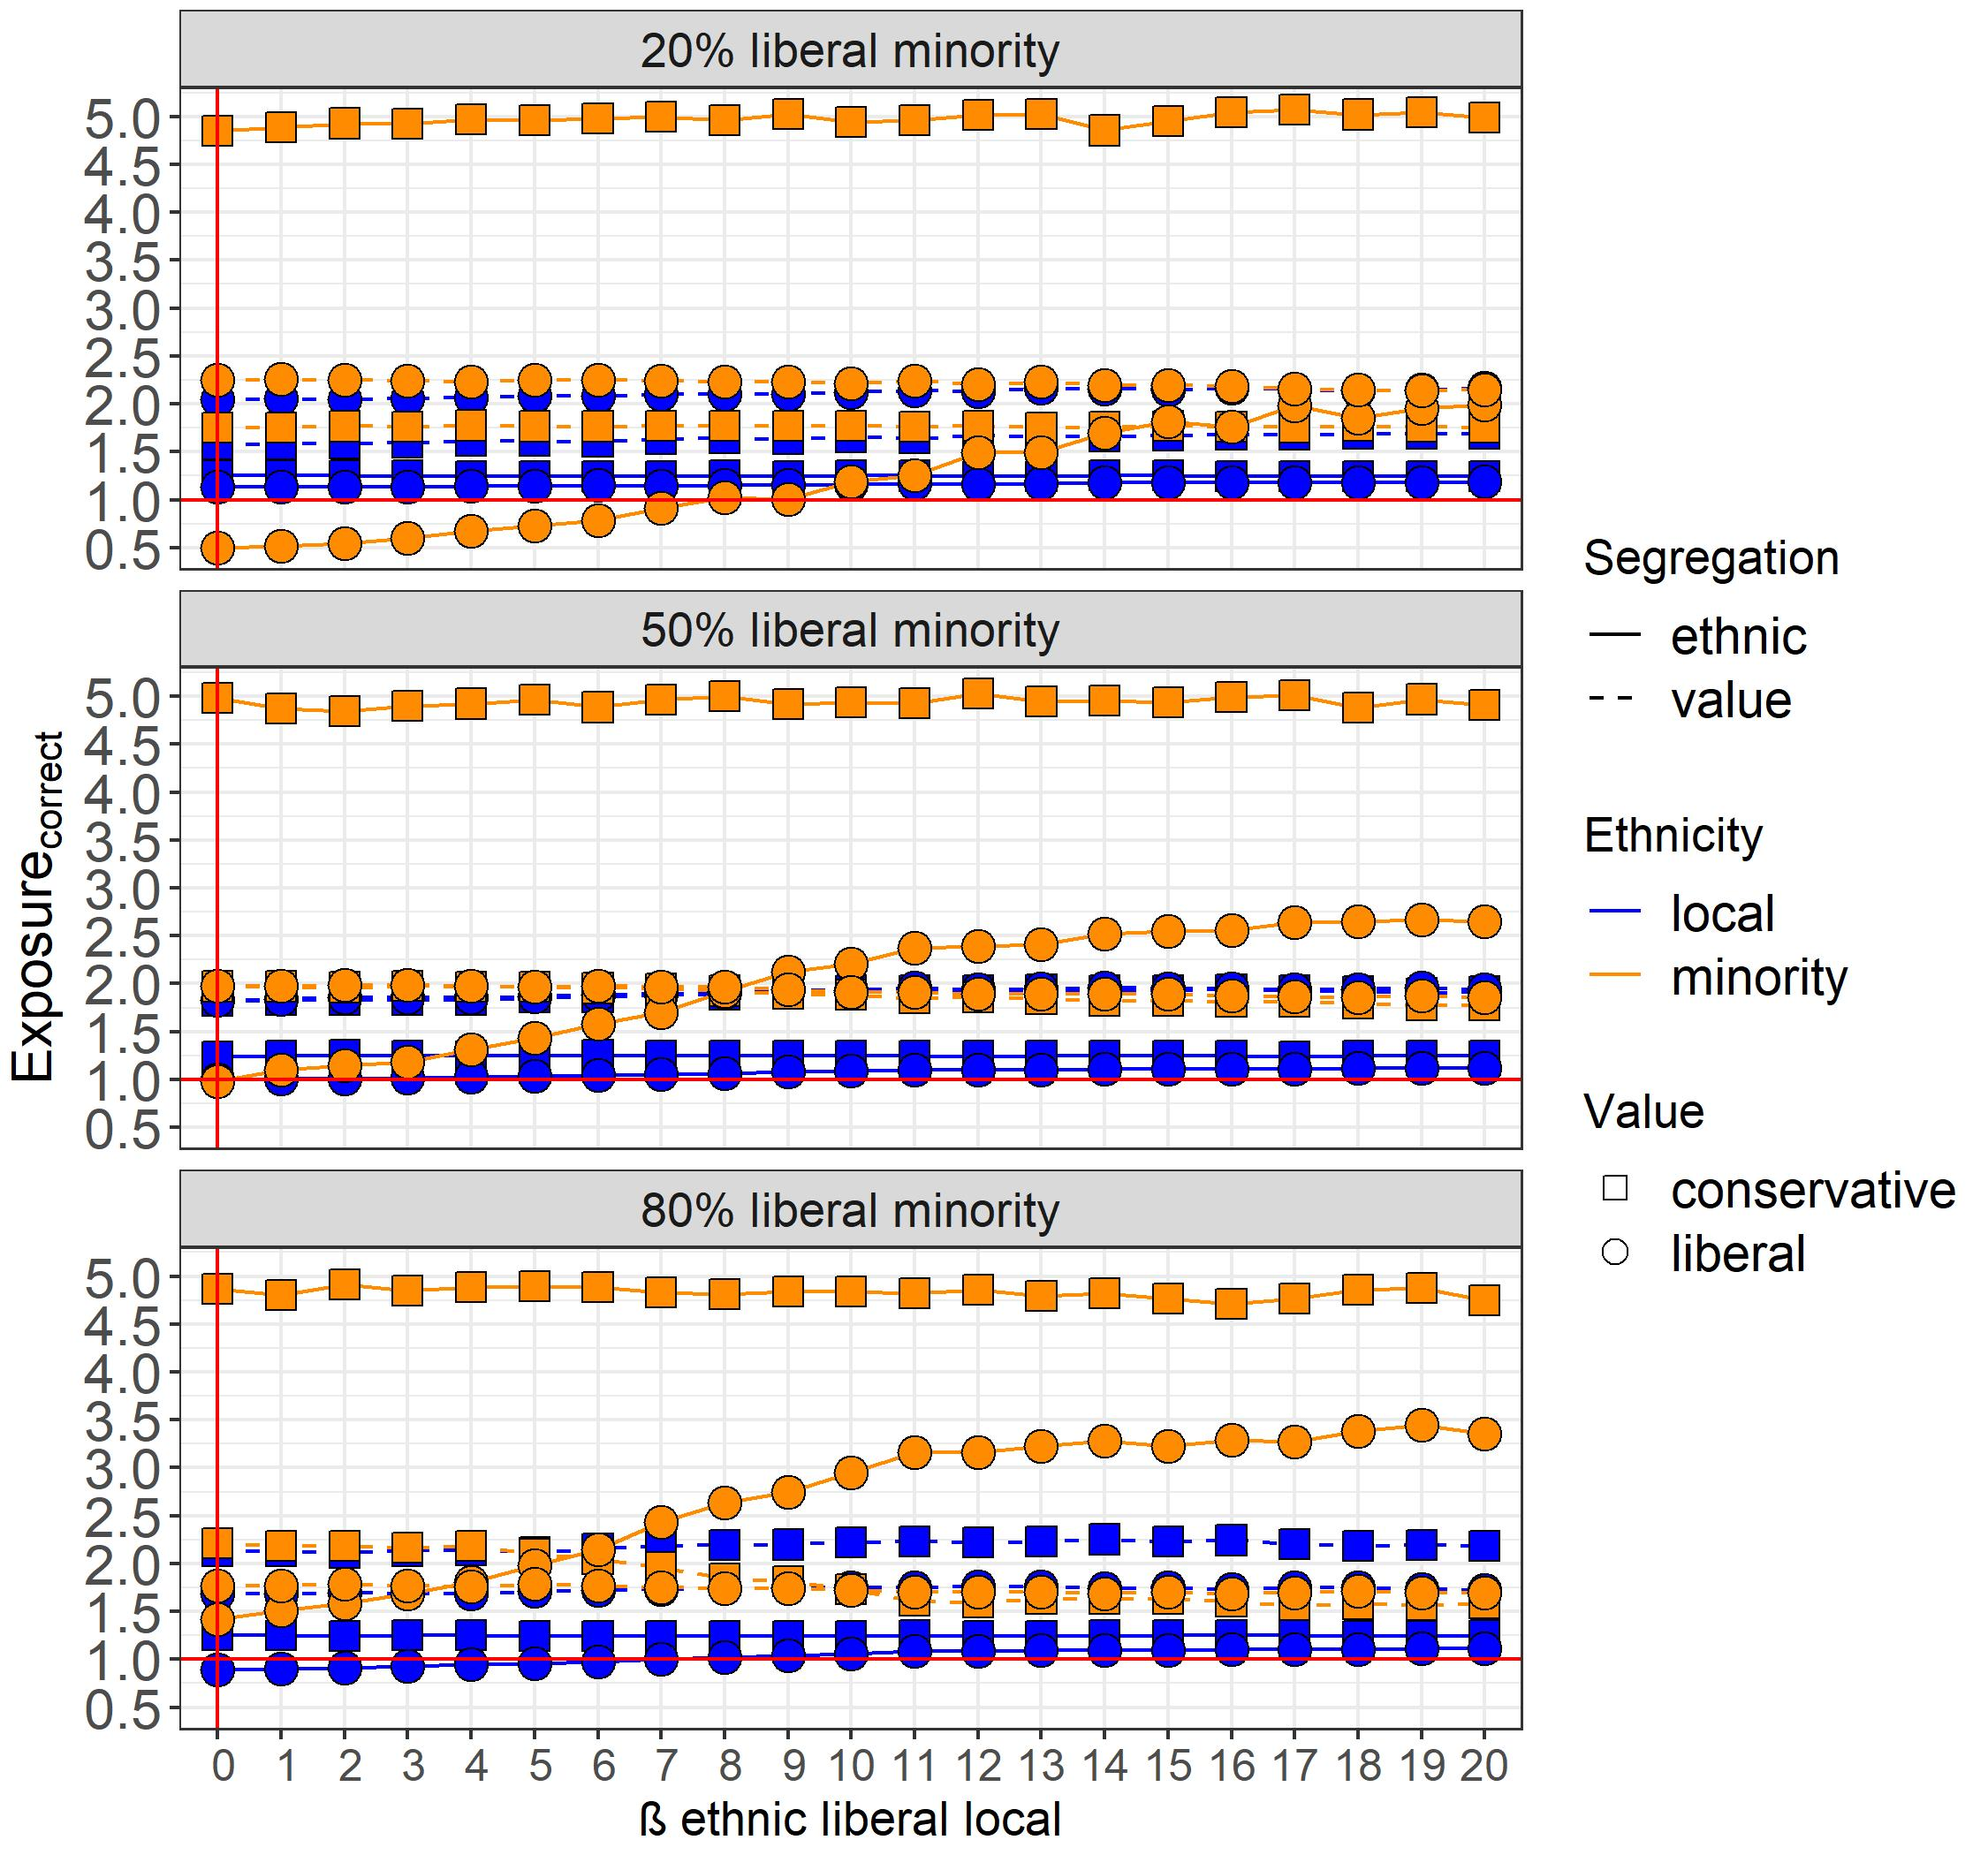
\includegraphics[scale=0.5]{material/figures/et_libloc.jpg}
    \caption{Interaction of increase ethnic preference of liberal locals and distribution of liberal minorities \rocco{to blend with Fig: \ref{fig:et_libmin}? now text treat differently}}
    \label{fig:et_libloc}
\end{figure} % etlibloc*min





\begin{figure}[H]
    \centering
    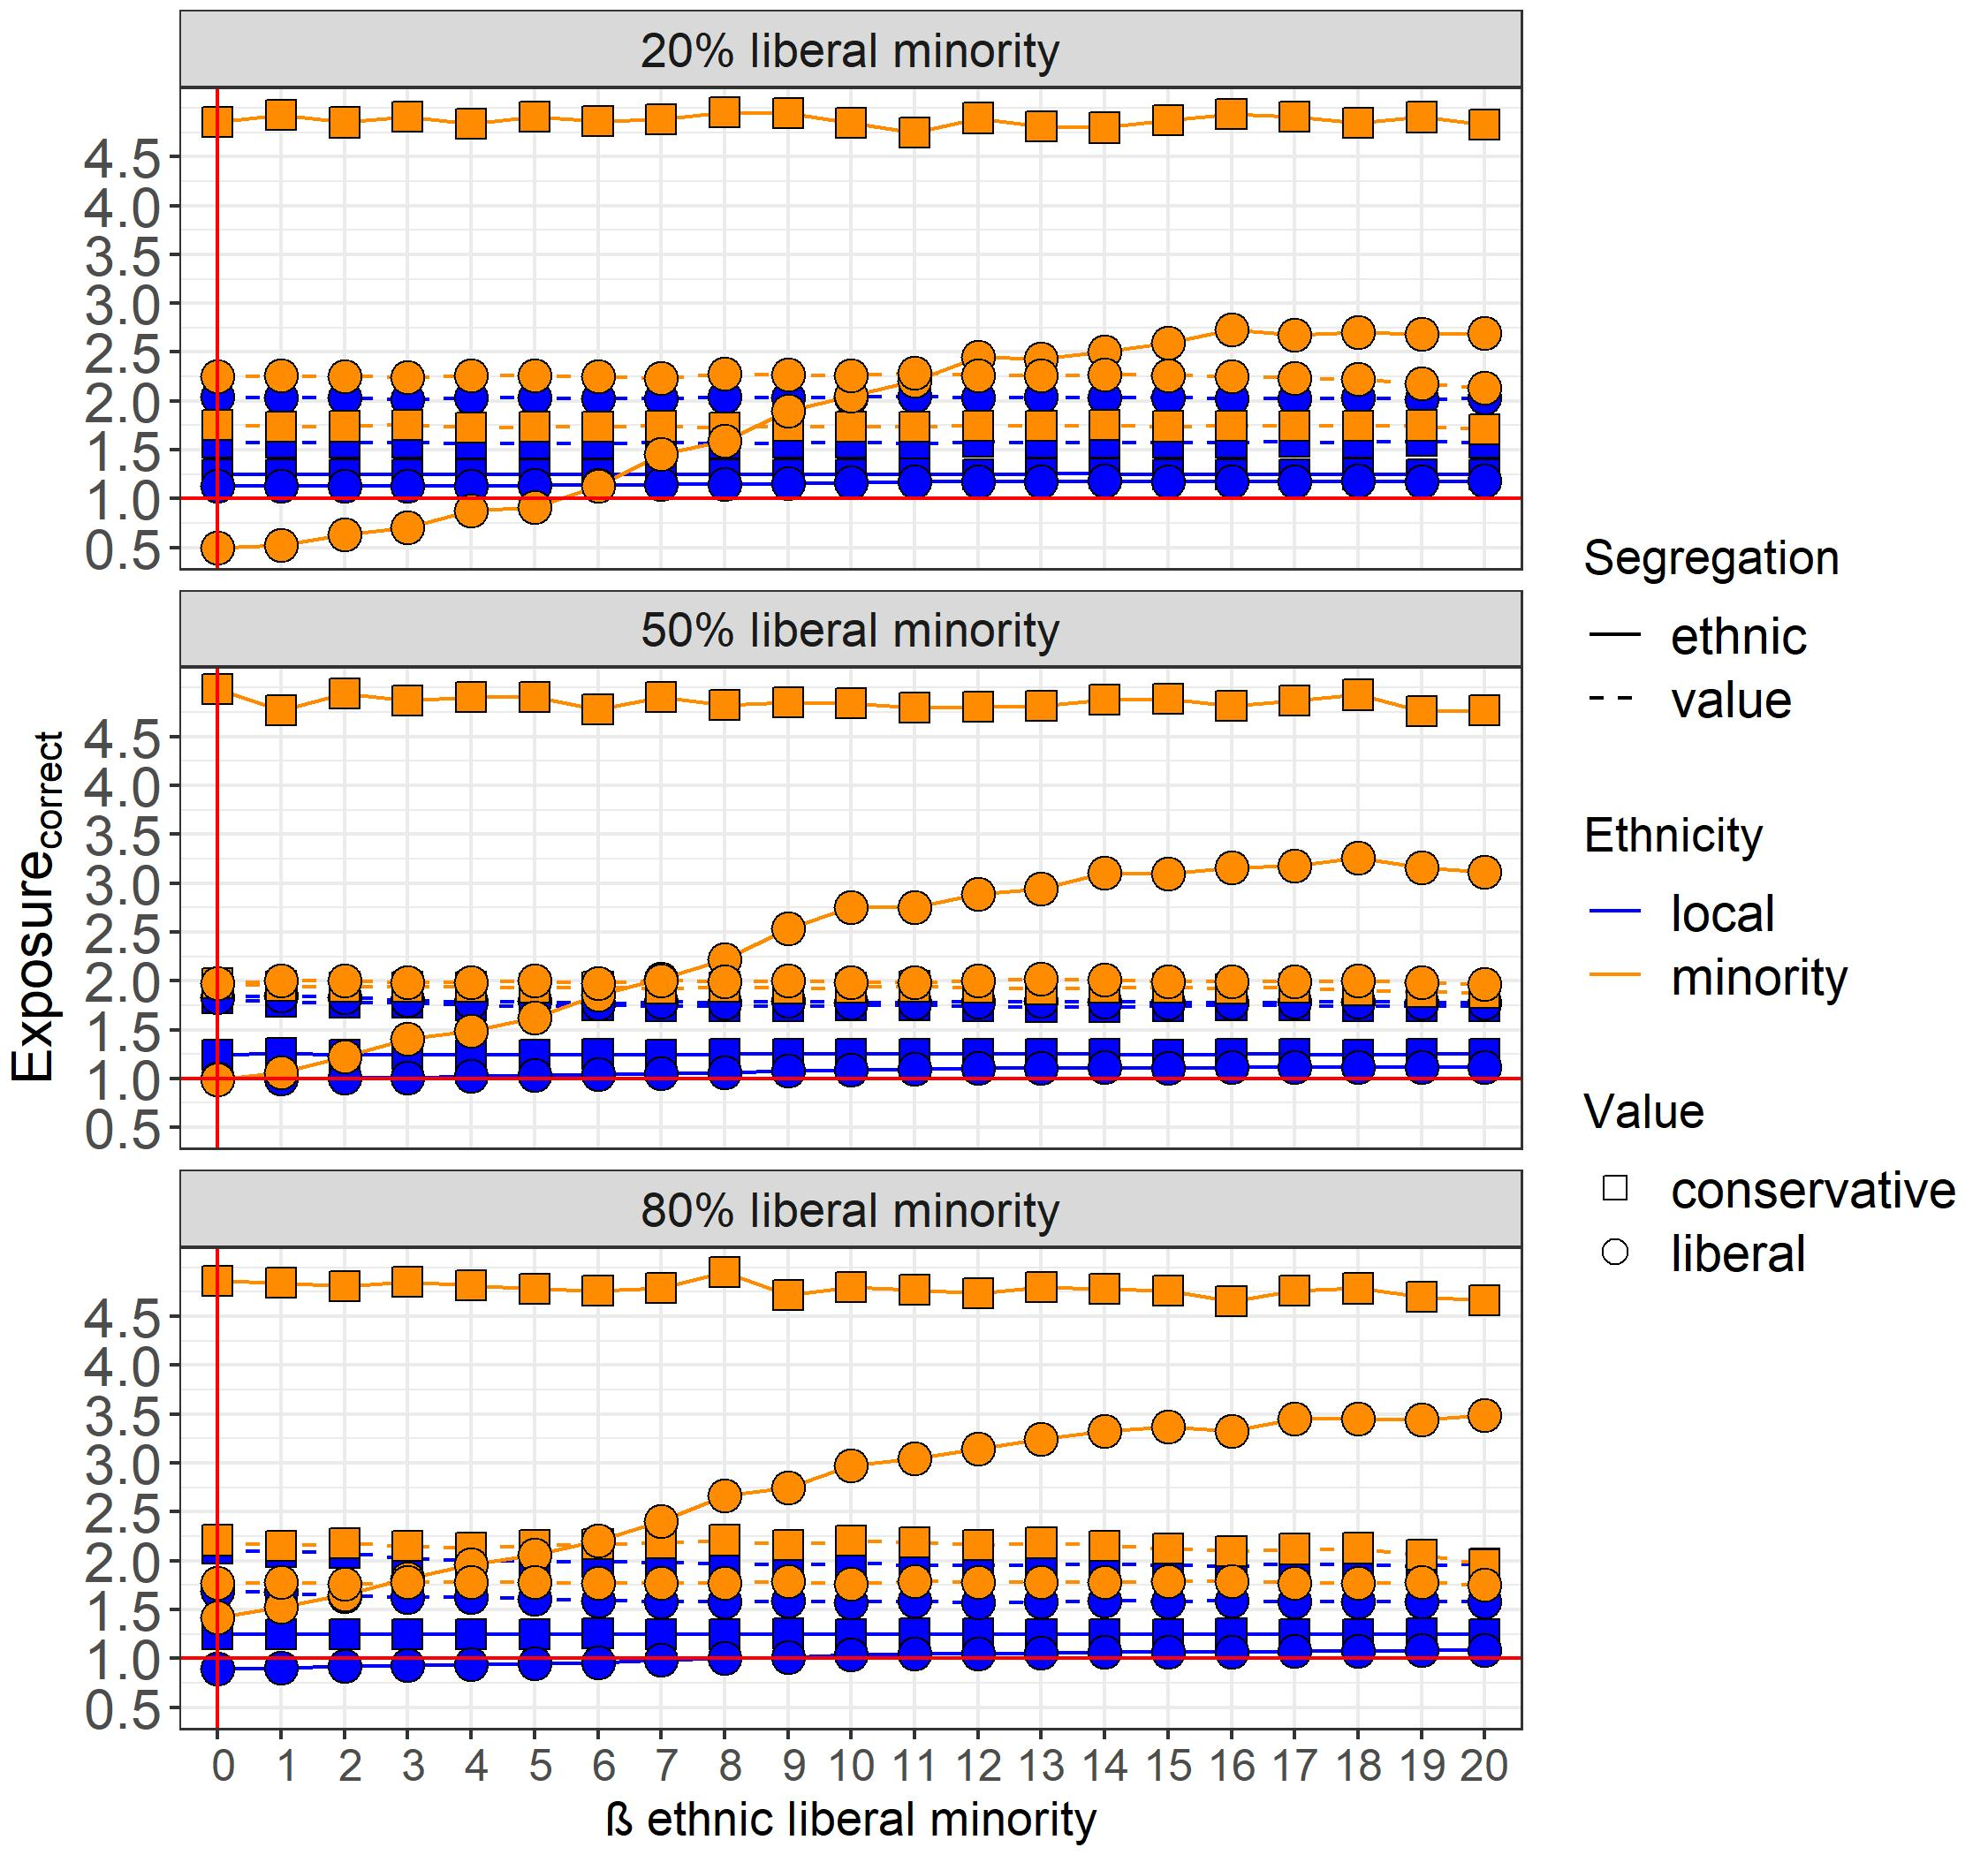
\includegraphics[scale=0.5]{material/figures/et_libmin.jpg}
    \caption{Interaction of increase ethnic preference of liberal minority and distribution of liberal minorities \rocco{to blend with Fig: \ref{fig:et_libloc}? now text treat differently}}
    \label{fig:et_libmin}
\end{figure} % etlibmin*min

\begin{figure}[H]
    \centering
    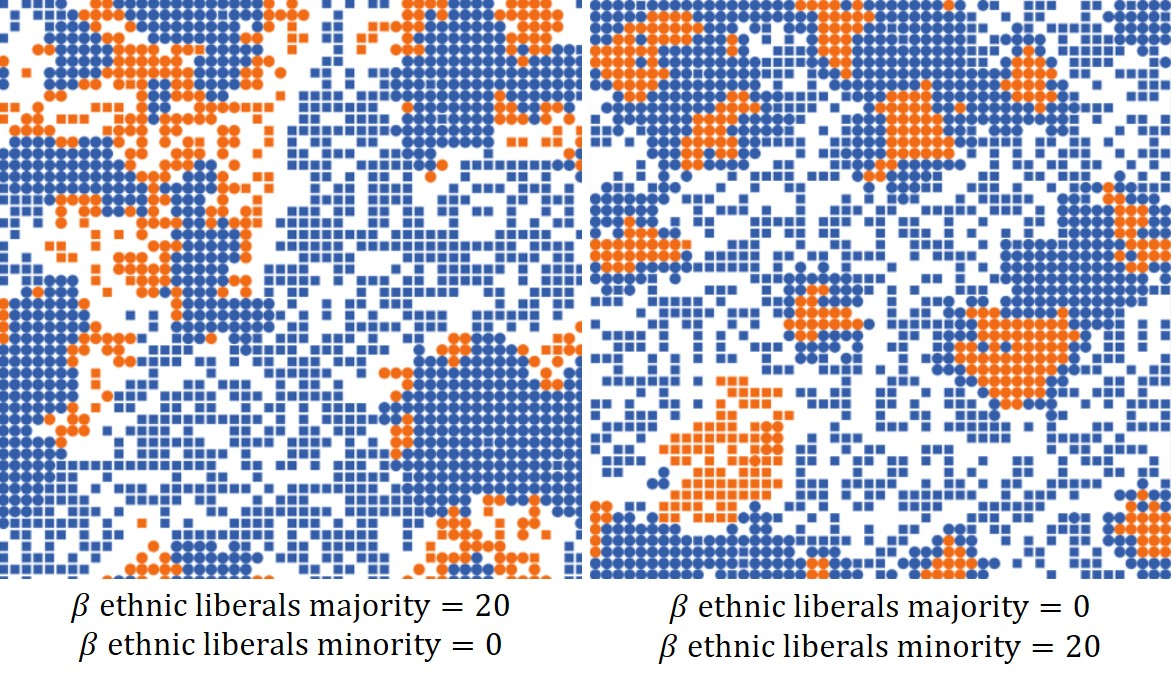
\includegraphics[scale=0.5]{material/figures/80_comp_eth.jpg}
    \caption{Comparison of ethnic preference of liberals majority (Fig: \ref{fig:et_libloc} and liberals minority \ref{fig:et_libmin} for $80 \%$ liberals minority} \rocco{If this is going to be included, to be better edited and merged with other figures}
    \label{fig:80_etlib}
\end{figure} % 80_etlib


\begin{figure}[H]
    \centering
    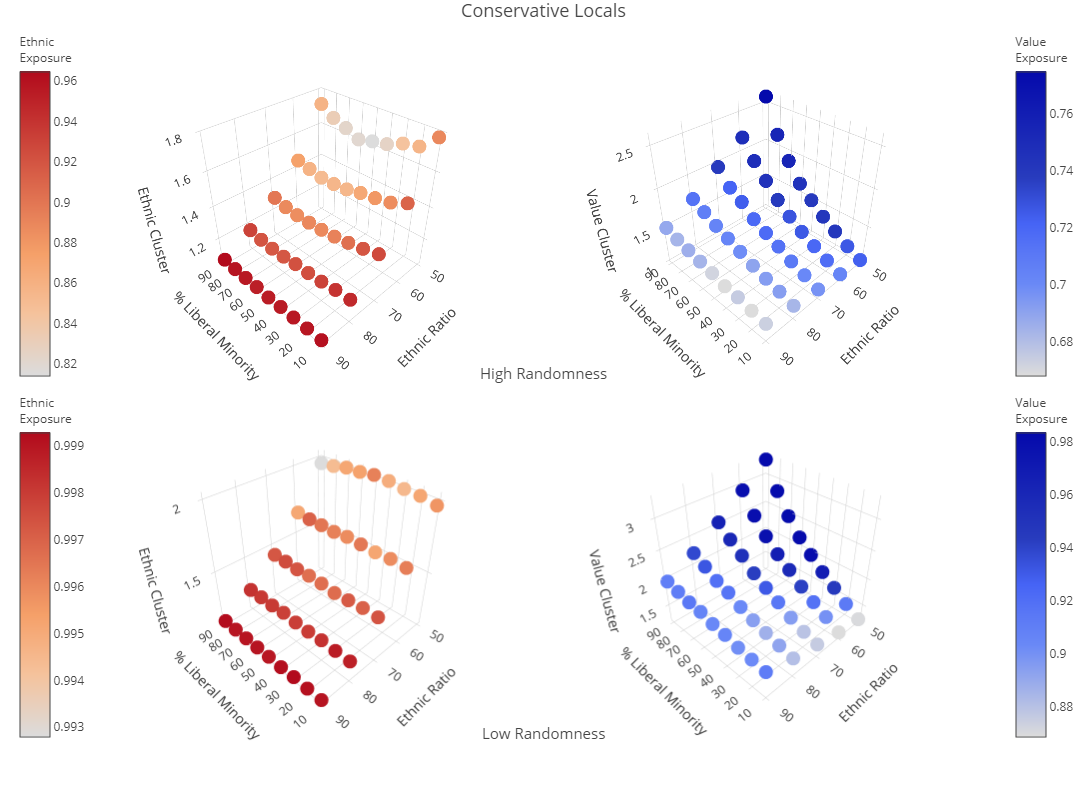
\includegraphics[scale=0.3]{material/figures/newplot.jpg}
    \caption{Test 3D}
    \label{fig:et_libloc}
\end{figure} % etlibloc*min


\section*{Conclusions and Discussions \rocco{working on} }

\rocco{more to the point: societies show lower ethnic segregation, increasing other dimensions (e.g. ses), and literature shows other characteristics matter $>$ acs2018 $>$ now discrete choice and other extension, in medias res; results similar to \textcite{paolillo2018}}
Schelling's model is often cited to describe how high levels of spatial ethnic segregation can persist in society even if people hold slight preference to live close to co-ethnics. However, the high complexity of current society challenge some assumption of  the model. In particular, people belong to different categories, both within and between ethnic groups, and literature suggesting ethnicity could be less relevant than other categories to define similarity preferences in relocation choice. In this paper we wanted to extend Schelling to these scenario. We built on \textcite{paolillo2018} extension of Schelling to the scenario of members of the same ethnic group sharing common attributes with out-groups and holding higher preference for either ethnic membership or secondary characteristics. We extend the model to discrete choice random utility models, testing on effect of different weights (level of randomness) of agents and letting agents hold both ethnic and value preference. Our results confirm some peculiarities of value similarity based on shared attributes across ethnic membership despite our change to the decisional process of agents.
First, value similarity can induce a by-product segregation of conservatives who do not care about secondary attributes. Second, value similarity form denser neighborhoods due to inclusion of co-values from both ethnic groups; neighborhoods become more resilient to fluctuations in neighborhood composition. As already observed in \textcite{paolillo2018} the tendency is to form robust neighborhood value homogeneous but ethnically integrated. 

% However, our results show who the definition of similarity based on shared characteristics might be not sufficient to guarantee spatial integration between groups. Even if people care about value similarity, provided they hold same preference (weight) for ethnic membership, segregation would still emerge and cause double segregation also within ethnic or social groups.

Most results are similar to \textcite{paolillo2018} because a thereshold = 0 equals to randomness $\beta = 0$ in terms of relocation decision of agents and aggregated results. However, inclusion of randomness, along with preference for both ethnic and value similarity, and senstivity to different group size, show different highlights on the segregation process.

Our results show who the definition of similarity based on shared characteristics might be not sufficient to guarantee spatial integration between groups. If people care about both ethnic and value similarity, full segregation for both dimension would lead to division of society in four group-types. However, lower determinism in the relocation choice can decrease segregation. If liberals become more ethnically conservatives, they would need higher preference to reach full ethnic segregation, as long as conservatives not care about secondary preference. On the contrary, value segregation of conservatives would not increase if they were to increase value preference, as long as liberals are enough to enact by-product value-segregation. This could explain why segregation by ses seems stronger than ethnic segregation \rocco{costs to be considered} and ethnic homogeneous neighborhoods are often also ses and educational homogeneous \rocco{link to double segregation in Fossett, not because of affordability, but because of by-product of other classes wanting to segregate}. Sensitivity analysis shows the role of relative sizes. First, effects due to majority are higher, this is evident from liberals majority who can cause more changes in the model. Even if liberals minority could cause the same mechanism, they don't reach a critical mass to do so. Relative size show how same preference in terms of weights can have different effect: for majority remaining in high ethnic exposure though not spatially segregating, while for minority higher spatial clustering emerges to satisfy even low preference. Segregation patterns of liberals: even if liberals of two ethnic groups recognize each other as similar, this would not translate into integrated neighborhoods because of relative sizes. The result shows ethnic assimilation of liberals minority separated from their co-ethnics with different secondary attributes. Only if distribution of liberals increases to a certain critical mass, the ethnic exposure of majority as effect of value similarity would diminish % alternative to ethnic assimilation of minority is majority counter-part to relocate randomly, then ethnic  segregation due to value preference
We show how integration can emerge from the condition where majority increase ethnic preference, through adaptation between liberals and conservatives of minority group  and the spatial configurations formed.




\rocco{to compare with Schelling: how segregation is a stable results, when and why in our model integration can emerge}
In Schelling, segregation as unstable condition results from all agents holding the same threshold (hold same preference) within spatial constraints and cascades that change neighborhood composition. In our results, segregation would equally emerge if agents hold high deterministic preference (higher $\beta$) for both dimensions. Integration will persist if agents hold random behavior for either or both dimensions, and the structural conditions of ethnic sizes and value distribution


Limits: a mix of linear combinations, all can be predicted, once the model is understood.


Next steps: to overcome tendency to segregation, a first step is to change the shape of utility function, along with the two-dimensional homophily behavior. \rocco{This links to the literature showing how segregation emerges also for integrationist preferences (Zhang, Van Rijt etc.) third paper of the dissertation I am working on}



\section*{Old notes and thoughts, to incorporate or delete}

\begin{itemize}

\item We focus on possible emerging patterns due to homophily preferences. This does not explain why people belonging to some categories might have some preferences over others. In the future, the project might include the individual determinants of homophily preferences,  e.g. correlating with social mobility intentions, life course approach, etc.

\item old intro: spatial segregation. Although such complex segregation scenarios result from a mix of preferences, constraints and resources \autocite{clark2015residential}, in this paper we concentrate on the role of preferences because core to Schelling’s dynamics to link individual behavior to change in segregation. In addition to ethnic preferences, we build on how people in diverse societies, belonging to different social distinctions, can adopt arbitrary criteria to define the limits of in-group inclusion, independent of ethnicity and attributing them different salience \autocite{albeda2018symbolic}.  

\item A common trait of most Western societies which have experienced decades of migration in-flows and further generations of children of migrants is that of super-diversity \autocite{vertovec2007super}. The concept refers not only to increased ethnic diversity, but also to the “diversification of diversity” \autocite[3, cfr Hollinger 1995]{martiniello2004combine}\autocite[cfr.]{hollinger1995beyond}, i.e. how diversity spans along different domains in addition to ethnicity, and how members of the same ethnic group can experience different rates of integration along such domains.  

\item About diversity in society: Further material I could not integrate properly in this line argument. I propose to move this towards the discussion section of the paper: This condition results not only from a mix of increased diversity and demographic changes accumulated through years \autocite{crul2016super} and categories of self-identification elaborated within each domain \autocite{vertovec2007super}, but also from inequalities in economic and cultural capital. On the last point, differences can emerge both between cohorts of the same ethnic group as result of integration policies adopted by countries  \autocite{crul2017upcoming}, and between individuals due to transmission within families and success in social mobility \autocite{Esser2010assimilation}.  
\end{itemize}

\section*{Appendix A - Additional Analysis}


\begin{figure}[H]
    \centering
    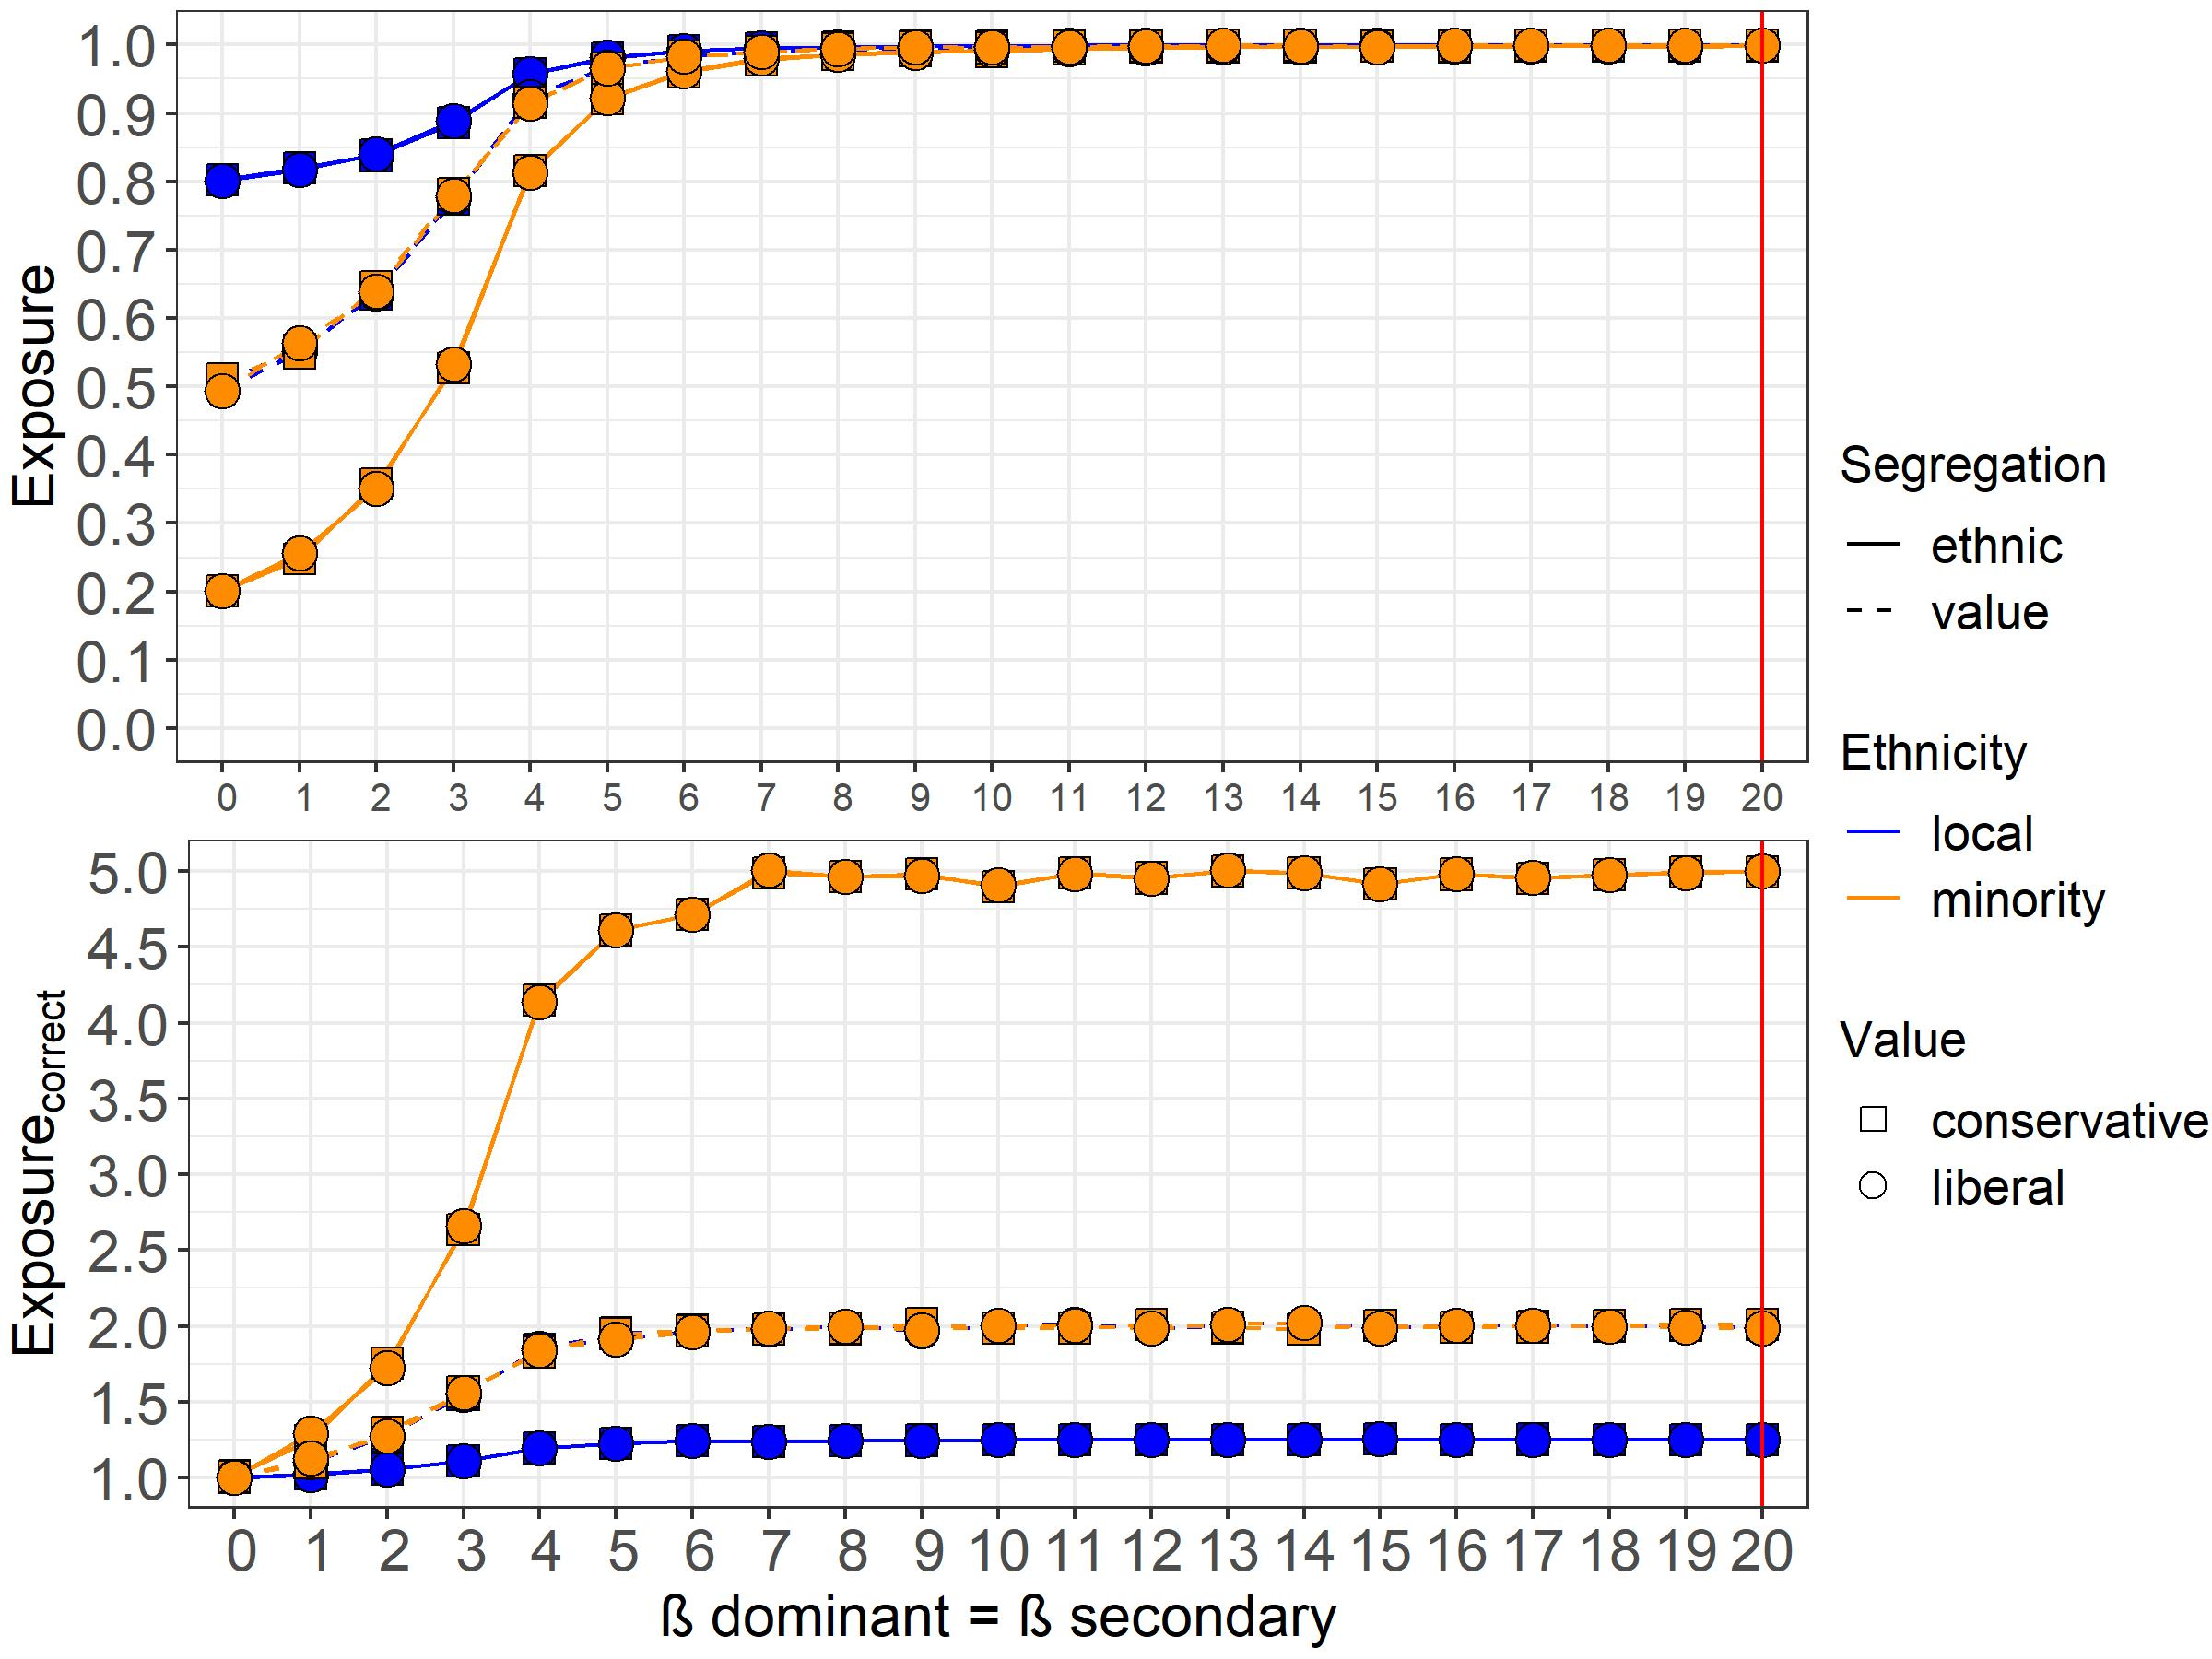
\includegraphics[scale=0.5]{material/figures/asym_all.jpg}
    \caption{Fig: \ref{fig:baseline} for ethnic asymmetry, $\beta \,dominant = \beta \,secondary$}
    \label{fig:etcnlc}
\end{figure} % etcnlc*min


\begin{figure}[H]
    \centering
    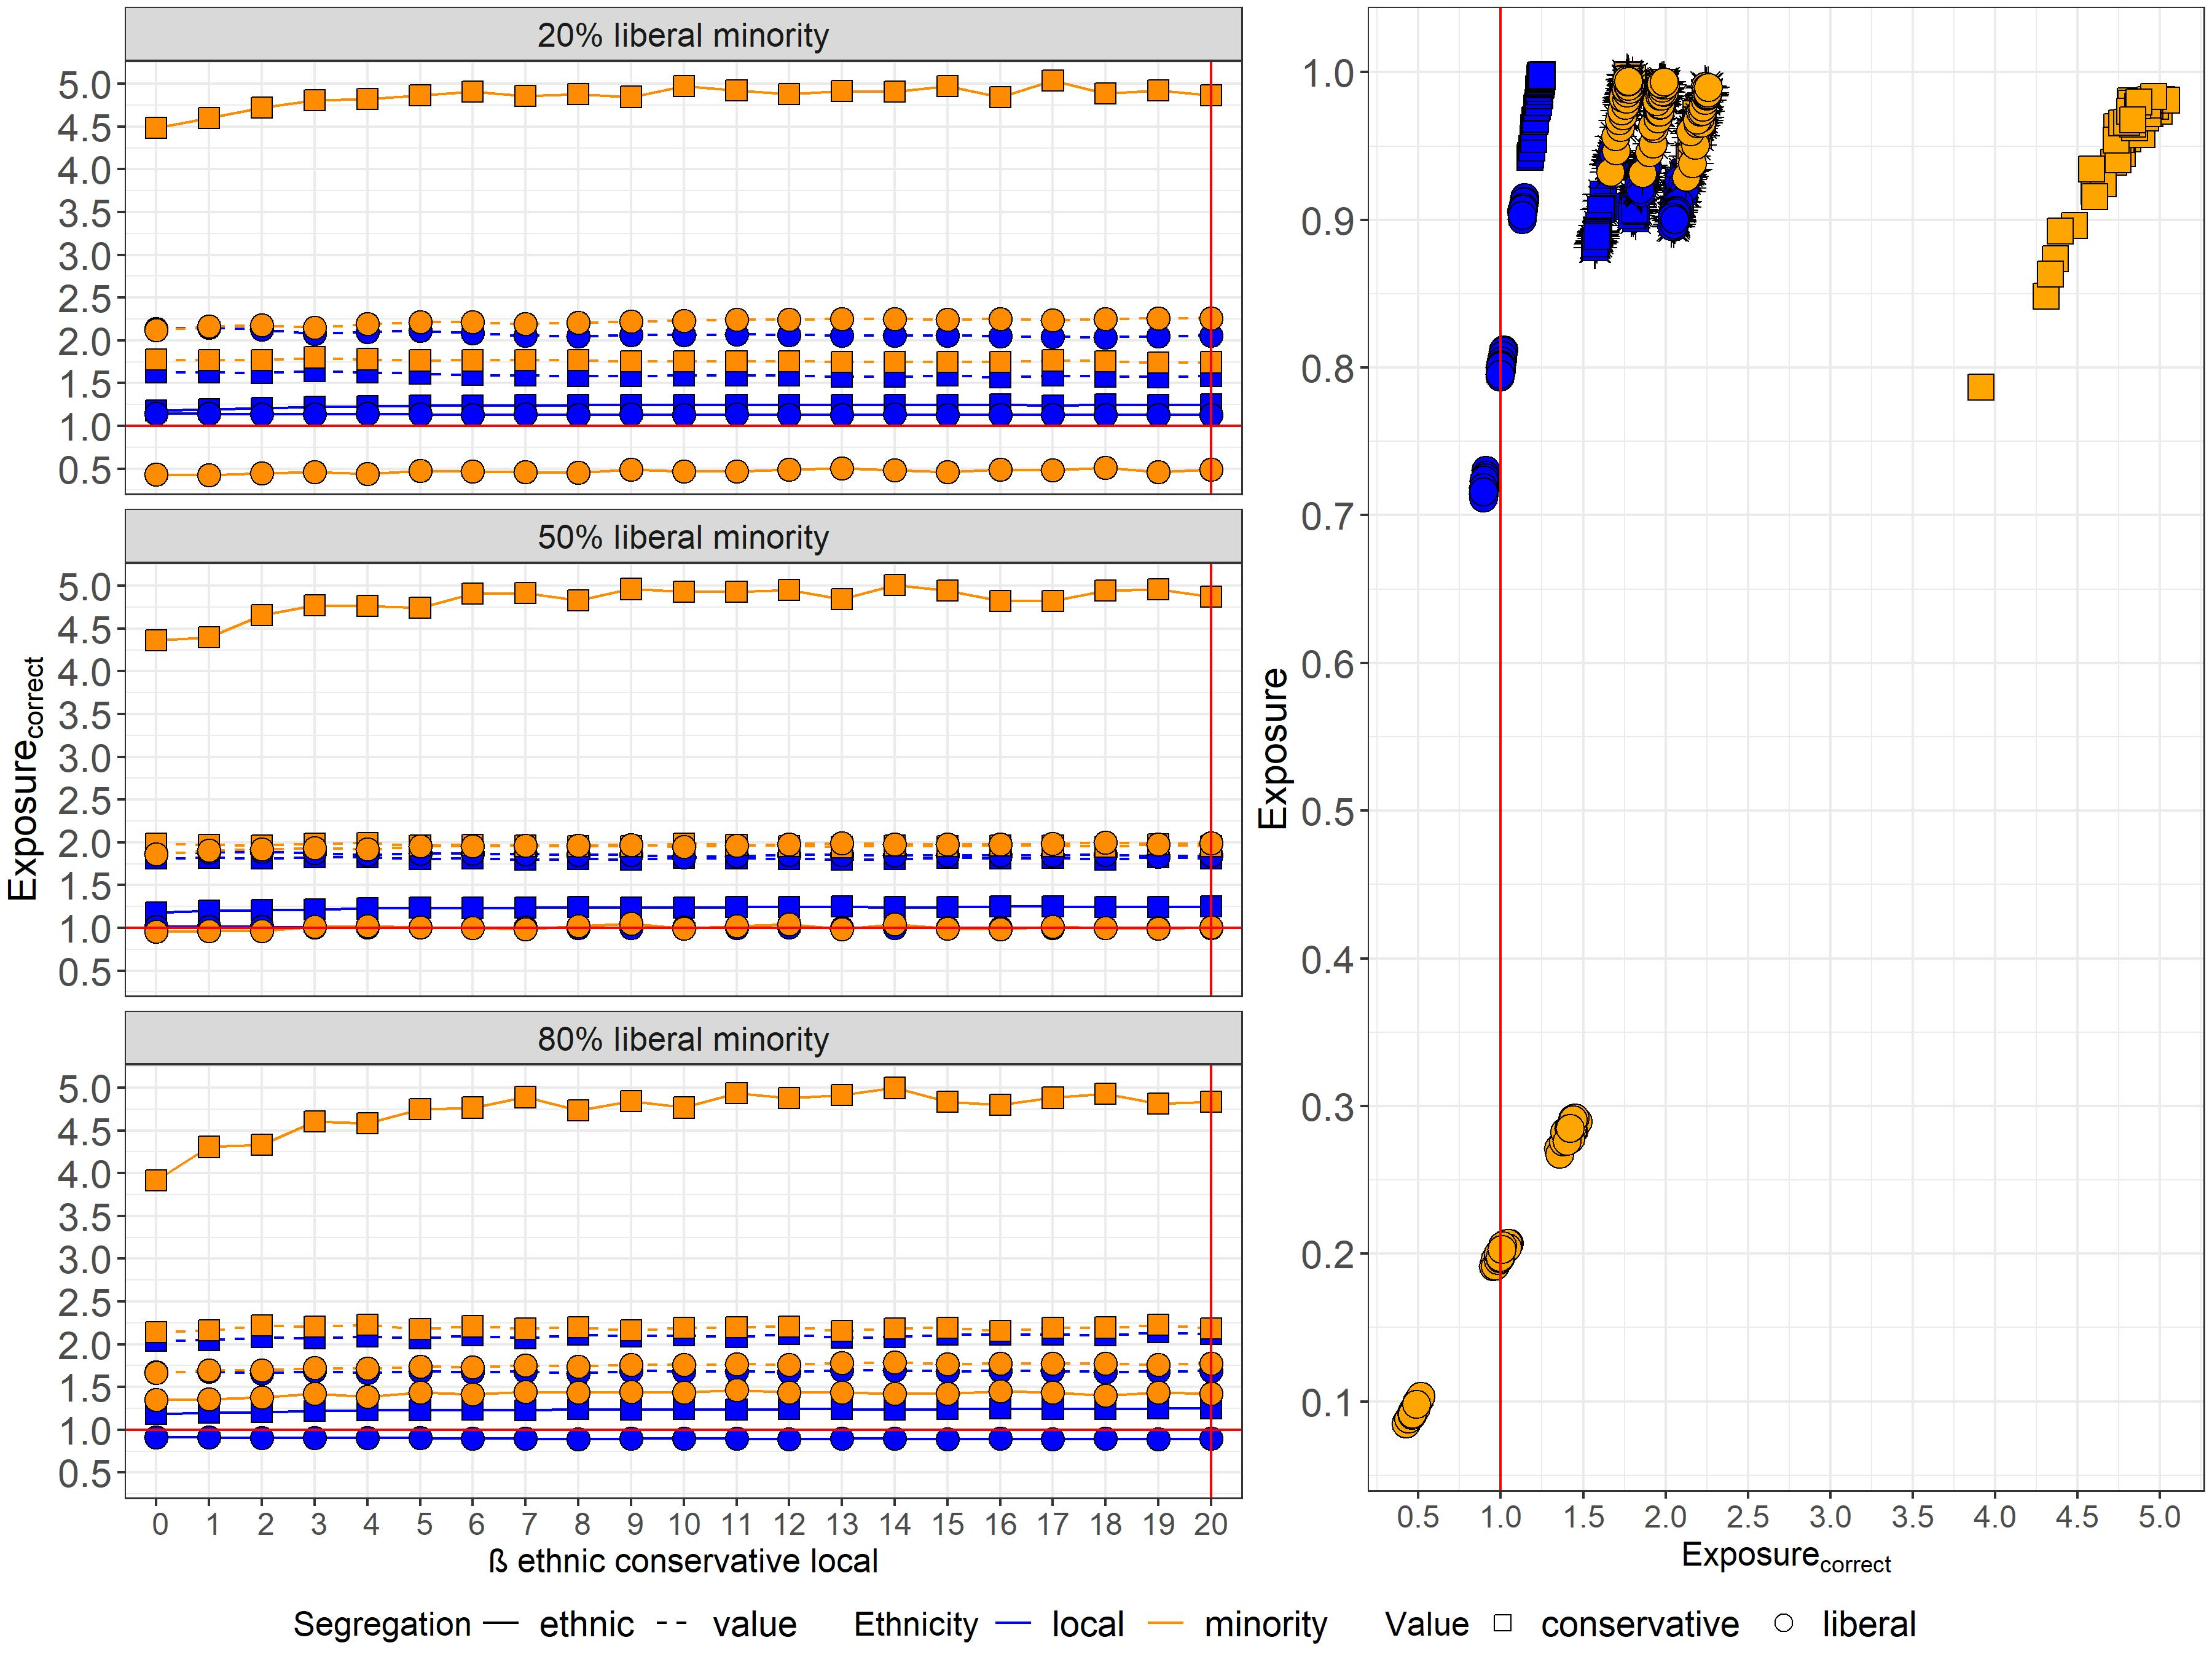
\includegraphics[scale=0.5]{material/figures/etcnlc.jpg}
    \caption{Interaction of ethnic preference of conservative locals and distribution of liberal minorities}
    \label{fig:etcnlc}
\end{figure} % etcnlc*min


\begin{figure}[H]
    \centering
    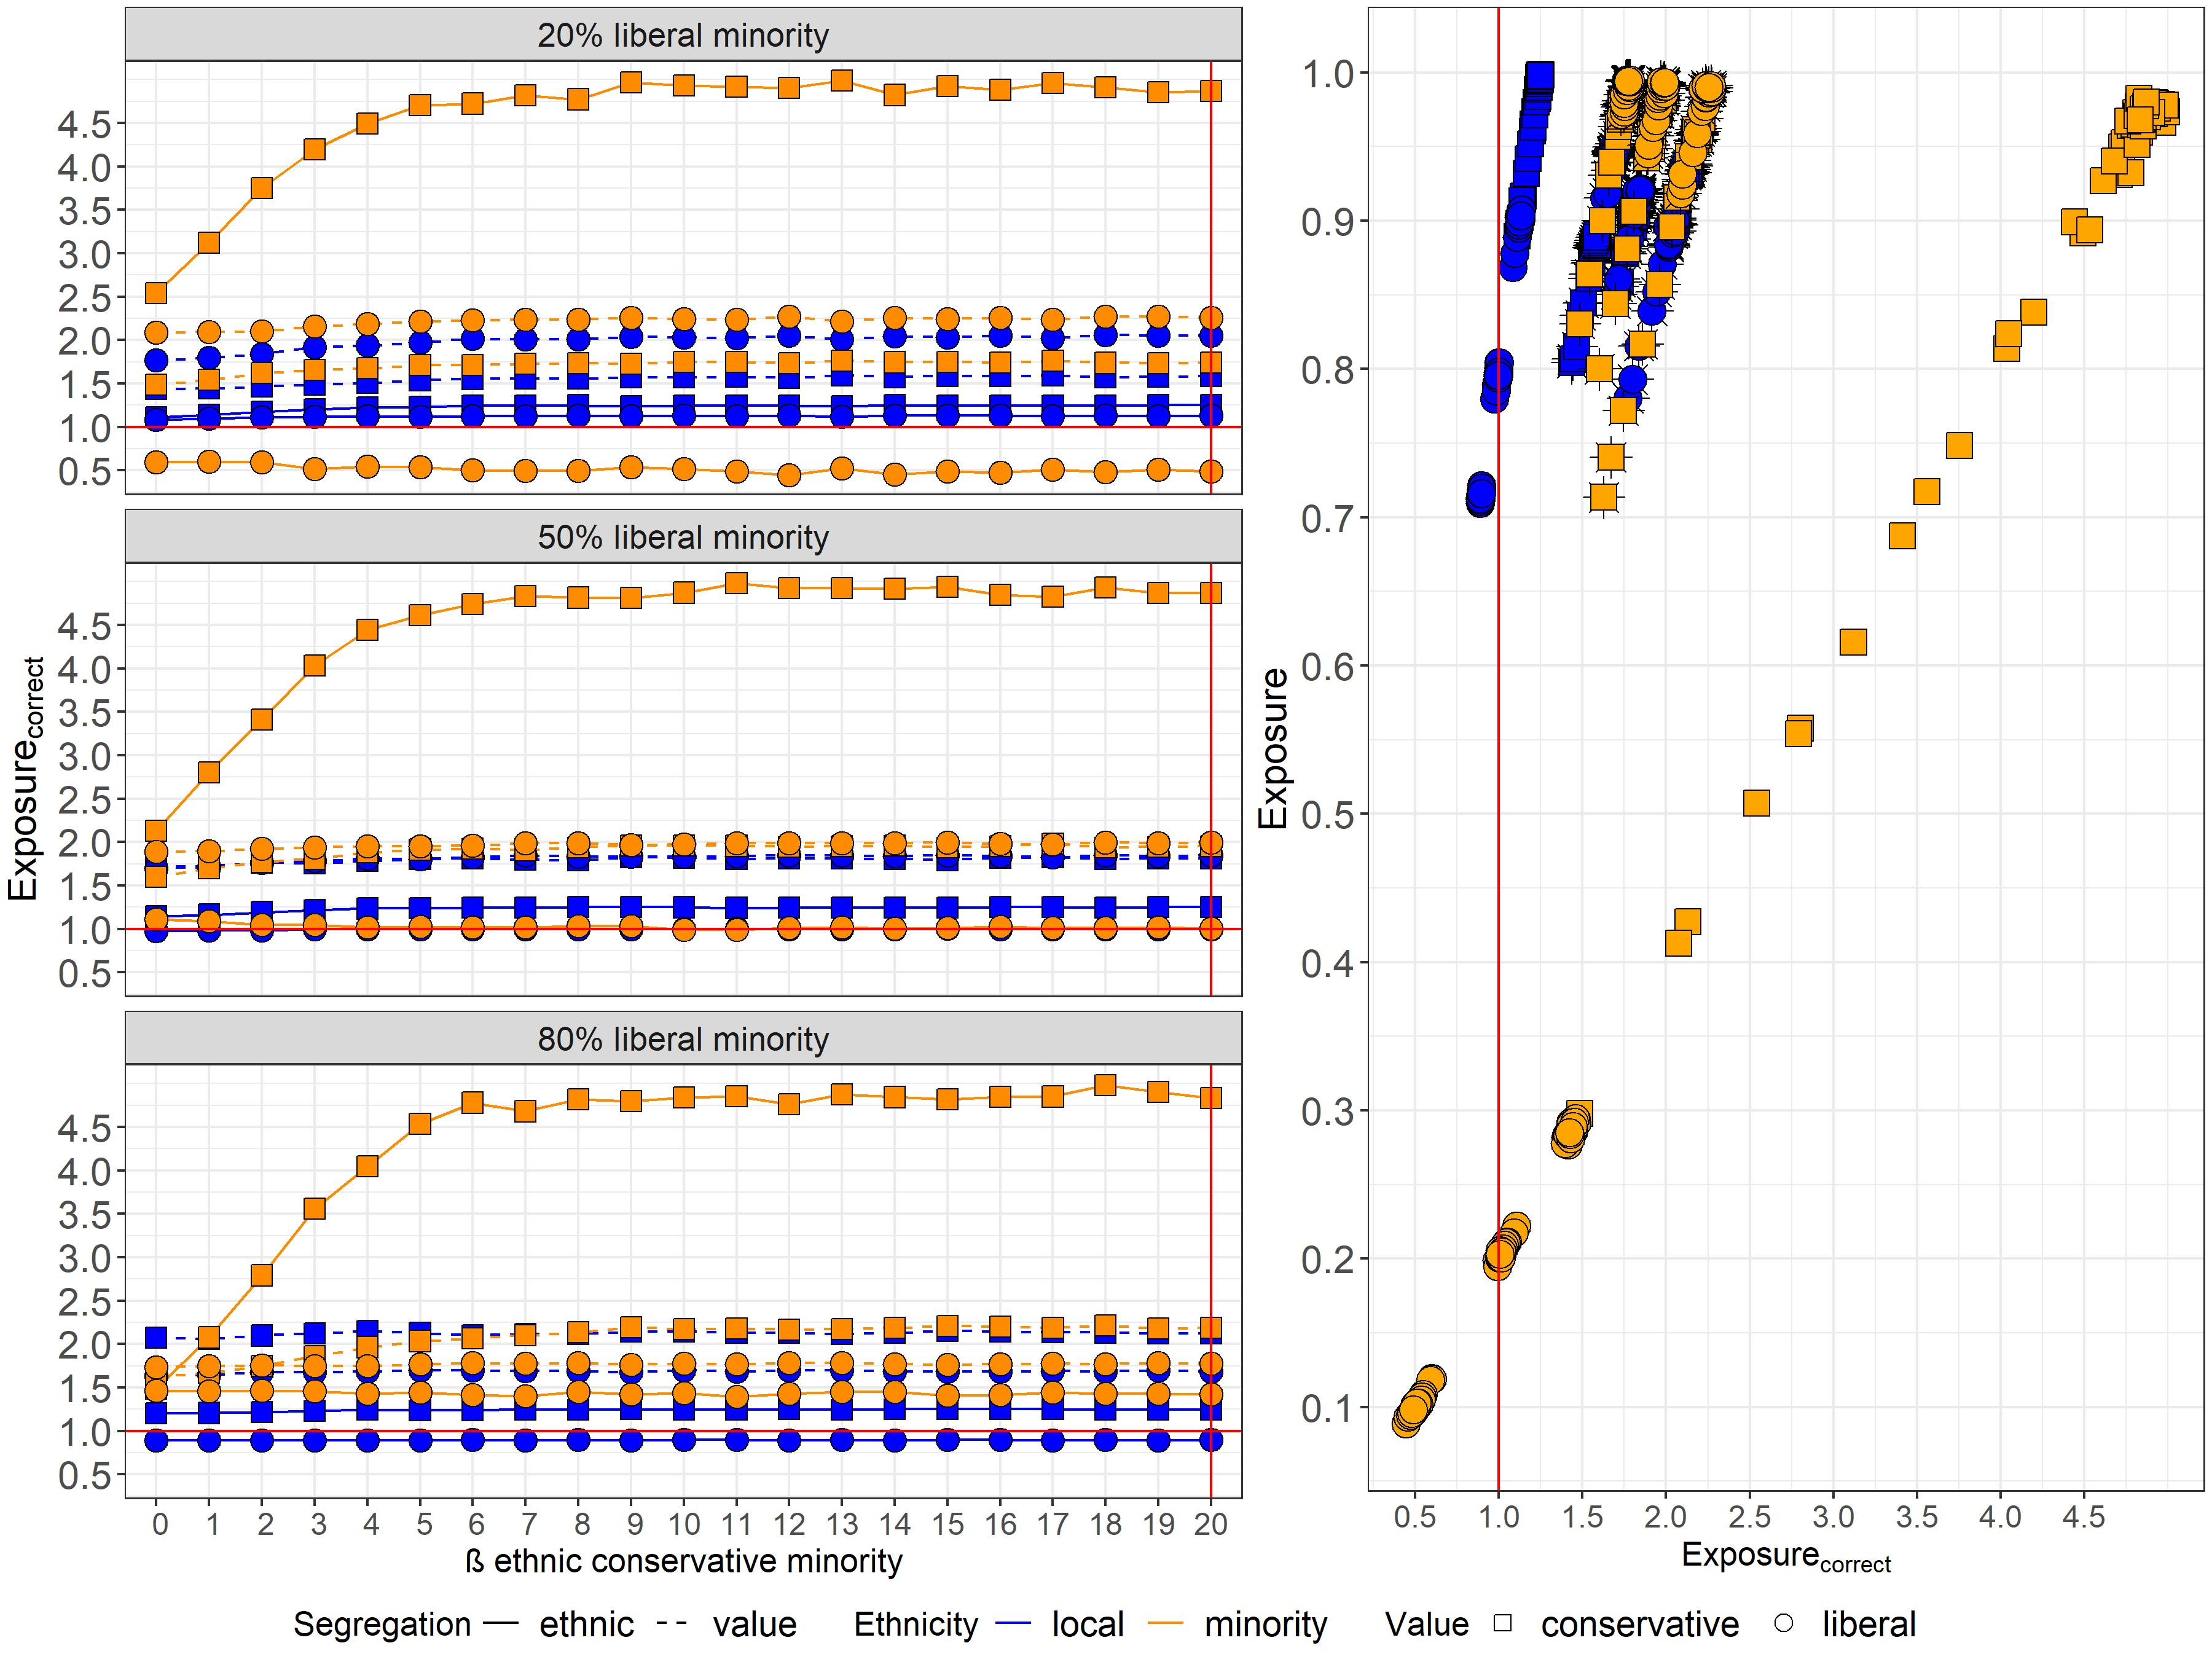
\includegraphics[scale=0.5]{material/figures/etcnmn.jpg}
    \caption{Interaction of ethnic preference of conservative minority and distribution of liberal minorities}
    \label{fig:etcnmn}
\end{figure} % etcnmnc*min

\section*{Appendix B - Robustness Analysis}


\begin{table}[H]
\scalebox{0.6}{
\begin{tabular}{|c|c|c|c|c|c|c|c|c|c|c|c|c|c|c|c|c|}
  \hline
  \multicolumn{17}{|c|}{Baseline condition}  \\\hline
 Preference &  \multicolumn{8}{|c|}{Ethnic Exposure} & \multicolumn{8}{|c|}{Value Exposure}   \\\hline
 & \multicolumn{4}{|c|}{Local} & \multicolumn{4}{|c|}{Minority}  & \multicolumn{4}{|c|}{Majority} & \multicolumn{4}{|c|}{Minority}  \\
 $\beta$ dom = $\beta$ sec & \multicolumn{2}{|c|}{Conservative} & \multicolumn{2}{|c|}{Liberal} 
& \multicolumn{2}{|c|}{Conservative} & \multicolumn{2}{|c|}{Liberal} & \multicolumn{2}{|c|}{Conservative} & \multicolumn{2}{|c|}{Liberal} 
& \multicolumn{2}{|c|}{Conservative} & \multicolumn{2}{|c|}{Liberal}\\
  & Mean & SD & Mean & SD & Mean & SD & Mean & SD & Mean & SD & Mean & SD & Mean & SD & Mean & SD\\
 \hline
   0 & 0.505 & 0.018 & 0.504 & 0.021 & 0.497 & 0.015 & 0.499 & 0.015 & 0.499 & 0.015 & 0.500 & 0.019 & 0.498 & 0.015 & 0.504 & 0.014 \\ 
     1 & 0.550 & 0.015 & 0.553 & 0.011 & 0.554 & 0.017 & 0.558 & 0.016 & 0.547 & 0.014 & 0.556 & 0.017 & 0.545 & 0.016 & 0.558 & 0.019 \\ 
     2 & 0.637 & 0.019 & 0.639 & 0.018 & 0.640 & 0.019 & 0.639 & 0.018 & 0.644 & 0.016 & 0.642 & 0.019 & 0.643 & 0.016 & 0.639 & 0.017 \\ 
     3 & 0.775 & 0.014 & 0.781 & 0.018 & 0.783 & 0.020 & 0.776 & 0.026 & 0.767 & 0.014 & 0.771 & 0.018 & 0.784 & 0.021 & 0.777 & 0.022 \\ 
     4 & 0.921 & 0.013 & 0.924 & 0.013 & 0.920 & 0.011 & 0.922 & 0.013 & 0.924 & 0.014 & 0.923 & 0.014 & 0.919 & 0.014 & 0.918 & 0.014 \\ 
     5 & 0.968 & 0.008 & 0.967 & 0.007 & 0.969 & 0.009 & 0.967 & 0.007 & 0.968 & 0.008 & 0.968 & 0.008 & 0.967 & 0.009 & 0.967 & 0.009 \\ 
     6 & 0.984 & 0.005 & 0.983 & 0.005 & 0.984 & 0.004 & 0.982 & 0.006 & 0.983 & 0.004 & 0.984 & 0.005 & 0.982 & 0.006 & 0.982 & 0.006 \\ 
     7 & 0.991 & 0.003 & 0.991 & 0.003 & 0.991 & 0.003 & 0.992 & 0.003 & 0.989 & 0.005 & 0.989 & 0.005 & 0.990 & 0.004 & 0.990 & 0.004 \\ 
     8 & 0.993 & 0.003 & 0.993 & 0.003 & 0.993 & 0.003 & 0.994 & 0.002 & 0.993 & 0.003 & 0.993 & 0.003 & 0.994 & 0.003 & 0.994 & 0.003 \\ 
     9 & 0.994 & 0.002 & 0.996 & 0.003 & 0.995 & 0.002 & 0.995 & 0.002 & 0.996 & 0.002 & 0.996 & 0.003 & 0.995 & 0.002 & 0.995 & 0.002 \\ 
    10 & 0.996 & 0.002 & 0.997 & 0.002 & 0.996 & 0.002 & 0.997 & 0.002 & 0.996 & 0.002 & 0.996 & 0.002 & 0.996 & 0.002 & 0.996 & 0.002 \\ 
    11 & 0.997 & 0.002 & 0.998 & 0.002 & 0.997 & 0.002 & 0.997 & 0.002 & 0.997 & 0.002 & 0.998 & 0.002 & 0.997 & 0.001 & 0.997 & 0.002 \\ 
    12 & 0.998 & 0.001 & 0.998 & 0.002 & 0.998 & 0.001 & 0.998 & 0.001 & 0.997 & 0.002 & 0.997 & 0.002 & 0.998 & 0.001 & 0.998 & 0.001 \\ 
    13 & 0.998 & 0.001 & 0.998 & 0.001 & 0.998 & 0.001 & 0.998 & 0.001 & 0.998 & 0.002 & 0.998 & 0.001 & 0.998 & 0.002 & 0.998 & 0.001 \\ 
    14 & 0.998 & 0.001 & 0.998 & 0.001 & 0.998 & 0.001 & 0.998 & 0.001 & 0.998 & 0.001 & 0.998 & 0.001 & 0.999 & 0.001 & 0.999 & 0.001 \\ 
    15 & 0.999 & 0.001 & 0.998 & 0.001 & 0.999 & 0.001 & 0.999 & 0.001 & 0.999 & 0.002 & 0.998 & 0.002 & 0.998 & 0.001 & 0.999 & 0.002 \\ 
    16 & 0.998 & 0.002 & 0.998 & 0.001 & 0.998 & 0.002 & 0.998 & 0.001 & 0.999 & 0.001 & 0.999 & 0.001 & 0.999 & 0.001 & 0.999 & 0.001 \\ 
    17 & 0.999 & 0.001 & 0.999 & 0.001 & 0.999 & 0.001 & 0.999 & 0.001 & 0.999 & 0.001 & 0.999 & 0.001 & 0.999 & 0.001 & 0.999 & 0.001 \\ 
    18 & 0.999 & 0.001 & 0.999 & 0.001 & 0.999 & 0.001 & 0.999 & 0.001 & 0.998 & 0.002 & 0.999 & 0.001 & 0.999 & 0.001 & 0.999 & 0.001 \\ 
    19 & 0.999 & 0.002 & 0.999 & 0.001 & 0.999 & 0.001 & 0.999 & 0.001 & 0.999 & 0.001 & 0.999 & 0.001 & 0.999 & 0.001 & 0.999 & 0.001 \\ 
    20 & 0.999 & 0.001 & 0.999 & 0.001 & 0.999 & 0.001 & 0.999 & 0.001 & 0.999 & 0.001 & 0.999 & 0.001 & 0.999 & 0.001 & 0.999 & 0.001 \\ 
   \hline
\end{tabular}
}

\caption{Robustness analysis referred to Fig: \ref{fig:baseline}}
\label{tab:baseline}
\end{table} % baseline

\begin{table}[H]
\scalebox{0.6}{


\begin{tabular}{|c|c|c|c|c|c|c|c|c|c|c|c|c|c|c|c|c|}
  \hline
  \multicolumn{17}{|c|}{Secondary preference = 0}  \\\hline
 Preference &  \multicolumn{8}{|c|}{Ethnic Exposure} & \multicolumn{8}{|c|}{Value Exposure}   \\\hline
 & \multicolumn{4}{|c|}{Majority} & \multicolumn{4}{|c|}{Minority}  & \multicolumn{4}{|c|}{Majority} & \multicolumn{4}{|c|}{Minority}  \\
 $\beta$ sec = 0 & \multicolumn{2}{|c|}{Conservative} & \multicolumn{2}{|c|}{Liberal} 
& \multicolumn{2}{|c|}{Conservative} & \multicolumn{2}{|c|}{Liberal} & \multicolumn{2}{|c|}{Conservative} & \multicolumn{2}{|c|}{Liberal} 
& \multicolumn{2}{|c|}{Conservative} & \multicolumn{2}{|c|}{Liberal}\\
  & Mean & SD & Mean & SD & Mean & SD & Mean & SD & Mean & SD & Mean & SD & Mean & SD & Mean & SD\\
 \hline
   0 & 0.505 & 0.018 & 0.504 & 0.021 & 0.497 & 0.015 & 0.499 & 0.015 & 0.499 & 0.015 & 0.500 & 0.019 & 0.498 & 0.015 & 0.504 & 0.014 \\ 
     1 & 0.538 & 0.018 & 0.513 & 0.015 & 0.530 & 0.015 & 0.508 & 0.010 & 0.519 & 0.015 & 0.526 & 0.017 & 0.517 & 0.021 & 0.528 & 0.016 \\ 
     2 & 0.585 & 0.010 & 0.516 & 0.014 & 0.589 & 0.015 & 0.519 & 0.017 & 0.550 & 0.015 & 0.559 & 0.014 & 0.549 & 0.015 & 0.557 & 0.014 \\ 
     3 & 0.642 & 0.013 & 0.521 & 0.009 & 0.643 & 0.017 & 0.524 & 0.013 & 0.591 & 0.016 & 0.602 & 0.016 & 0.593 & 0.015 & 0.604 & 0.015 \\ 
     4 & 0.725 & 0.019 & 0.517 & 0.021 & 0.720 & 0.016 & 0.534 & 0.017 & 0.664 & 0.026 & 0.671 & 0.017 & 0.648 & 0.019 & 0.672 & 0.014 \\ 
     5 & 0.819 & 0.022 & 0.517 & 0.021 & 0.815 & 0.017 & 0.529 & 0.023 & 0.748 & 0.031 & 0.757 & 0.021 & 0.735 & 0.025 & 0.759 & 0.019 \\ 
     6 & 0.906 & 0.012 & 0.515 & 0.015 & 0.904 & 0.013 & 0.516 & 0.022 & 0.843 & 0.024 & 0.857 & 0.014 & 0.840 & 0.024 & 0.858 & 0.014 \\ 
     7 & 0.946 & 0.005 & 0.510 & 0.018 & 0.945 & 0.008 & 0.512 & 0.014 & 0.894 & 0.011 & 0.906 & 0.012 & 0.889 & 0.019 & 0.904 & 0.012 \\ 
     8 & 0.964 & 0.005 & 0.502 & 0.023 & 0.963 & 0.007 & 0.515 & 0.021 & 0.924 & 0.015 & 0.933 & 0.008 & 0.922 & 0.015 & 0.935 & 0.008 \\ 
     9 & 0.978 & 0.005 & 0.509 & 0.019 & 0.977 & 0.003 & 0.506 & 0.022 & 0.944 & 0.011 & 0.952 & 0.005 & 0.943 & 0.010 & 0.951 & 0.007 \\ 
    10 & 0.983 & 0.004 & 0.504 & 0.016 & 0.982 & 0.004 & 0.504 & 0.020 & 0.954 & 0.012 & 0.960 & 0.009 & 0.951 & 0.009 & 0.960 & 0.007 \\ 
    11 & 0.986 & 0.004 & 0.507 & 0.025 & 0.986 & 0.004 & 0.504 & 0.017 & 0.959 & 0.011 & 0.966 & 0.006 & 0.959 & 0.010 & 0.966 & 0.006 \\ 
    12 & 0.987 & 0.003 & 0.502 & 0.020 & 0.988 & 0.004 & 0.502 & 0.015 & 0.963 & 0.009 & 0.972 & 0.007 & 0.965 & 0.008 & 0.971 & 0.004 \\ 
    13 & 0.991 & 0.003 & 0.506 & 0.023 & 0.991 & 0.004 & 0.505 & 0.022 & 0.970 & 0.010 & 0.976 & 0.006 & 0.969 & 0.008 & 0.975 & 0.004 \\ 
    14 & 0.992 & 0.003 & 0.501 & 0.016 & 0.992 & 0.002 & 0.502 & 0.018 & 0.970 & 0.009 & 0.976 & 0.007 & 0.972 & 0.005 & 0.977 & 0.004 \\ 
    15 & 0.993 & 0.003 & 0.502 & 0.017 & 0.993 & 0.002 & 0.500 & 0.022 & 0.972 & 0.007 & 0.980 & 0.005 & 0.975 & 0.009 & 0.980 & 0.007 \\ 
    16 & 0.994 & 0.002 & 0.501 & 0.024 & 0.994 & 0.002 & 0.506 & 0.024 & 0.976 & 0.008 & 0.981 & 0.007 & 0.973 & 0.009 & 0.978 & 0.006 \\ 
    17 & 0.995 & 0.002 & 0.498 & 0.019 & 0.995 & 0.002 & 0.509 & 0.018 & 0.977 & 0.007 & 0.983 & 0.005 & 0.977 & 0.007 & 0.982 & 0.005 \\ 
    18 & 0.994 & 0.002 & 0.502 & 0.014 & 0.995 & 0.003 & 0.497 & 0.018 & 0.975 & 0.008 & 0.982 & 0.005 & 0.977 & 0.007 & 0.982 & 0.005 \\ 
    19 & 0.995 & 0.002 & 0.498 & 0.018 & 0.996 & 0.002 & 0.507 & 0.016 & 0.976 & 0.008 & 0.982 & 0.005 & 0.978 & 0.005 & 0.984 & 0.004 \\ 
    20 & 0.996 & 0.003 & 0.507 & 0.020 & 0.996 & 0.002 & 0.499 & 0.019 & 0.979 & 0.006 & 0.985 & 0.004 & 0.980 & 0.008 & 0.986 & 0.005 \\ 
   \hline
\end{tabular}
}

\caption{Robustness analysis referred to Fig: \ref{fig:sec_0}}
\label{tab:sec_0}
\end{table} % secondary = 0

\begin{table}[H]
\scalebox{0.6}{
\begin{tabular}{|c|c|c|c|c|c|c|c|c|c|c|c|c|c|c|c|c|}
  \hline
  \multicolumn{17}{|c|}{Baseline: sensitivity to value liberal}  \\\hline
 Preference &  \multicolumn{8}{|c|}{Ethnic Exposure} & \multicolumn{8}{|c|}{Value Exposure}   \\\hline
 & \multicolumn{4}{|c|}{Majority} & \multicolumn{4}{|c|}{Minority}  & \multicolumn{4}{|c|}{Majority} & \multicolumn{4}{|c|}{Minority}  \\
 $\beta$ dom & \multicolumn{2}{|c|}{Conservative} & \multicolumn{2}{|c|}{Liberal} 
& \multicolumn{2}{|c|}{Conservative} & \multicolumn{2}{|c|}{Liberal} & \multicolumn{2}{|c|}{Conservative} & \multicolumn{2}{|c|}{Liberal} 
& \multicolumn{2}{|c|}{Conservative} & \multicolumn{2}{|c|}{Liberal}\\
 liberal & Mean & SD & Mean & SD & Mean & SD & Mean & SD & Mean & SD & Mean & SD & Mean & SD & Mean & SD\\
 \hline
   0 & 0.498 & 0.012 & 0.494 & 0.012 & 0.498 & 0.018 & 0.501 & 0.016 & 0.506 & 0.013 & 0.497 & 0.018 & 0.504 & 0.019 & 0.499 & 0.012 \\ 
     1 & 0.503 & 0.019 & 0.501 & 0.012 & 0.491 & 0.015 & 0.493 & 0.013 & 0.523 & 0.011 & 0.528 & 0.016 & 0.517 & 0.015 & 0.529 & 0.018 \\ 
     2 & 0.498 & 0.019 & 0.494 & 0.012 & 0.500 & 0.021 & 0.499 & 0.018 & 0.544 & 0.015 & 0.561 & 0.014 & 0.544 & 0.010 & 0.562 & 0.013 \\ 
     3 & 0.499 & 0.016 & 0.498 & 0.012 & 0.502 & 0.019 & 0.497 & 0.016 & 0.578 & 0.014 & 0.592 & 0.018 & 0.579 & 0.013 & 0.589 & 0.013 \\ 
     4 & 0.497 & 0.019 & 0.501 & 0.017 & 0.497 & 0.018 & 0.495 & 0.019 & 0.615 & 0.011 & 0.636 & 0.018 & 0.614 & 0.016 & 0.634 & 0.015 \\ 
     5 & 0.489 & 0.019 & 0.497 & 0.015 & 0.507 & 0.014 & 0.501 & 0.017 & 0.656 & 0.011 & 0.680 & 0.014 & 0.657 & 0.012 & 0.676 & 0.019 \\ 
     6 & 0.502 & 0.015 & 0.505 & 0.013 & 0.490 & 0.020 & 0.494 & 0.020 & 0.699 & 0.013 & 0.718 & 0.018 & 0.699 & 0.012 & 0.722 & 0.016 \\ 
     7 & 0.500 & 0.014 & 0.503 & 0.018 & 0.500 & 0.018 & 0.504 & 0.016 & 0.763 & 0.024 & 0.788 & 0.016 & 0.764 & 0.021 & 0.788 & 0.015 \\ 
     8 & 0.499 & 0.021 & 0.495 & 0.018 & 0.500 & 0.016 & 0.500 & 0.017 & 0.824 & 0.020 & 0.843 & 0.015 & 0.825 & 0.021 & 0.845 & 0.014 \\ 
     9 & 0.508 & 0.022 & 0.497 & 0.012 & 0.493 & 0.024 & 0.495 & 0.019 & 0.872 & 0.019 & 0.883 & 0.012 & 0.874 & 0.015 & 0.888 & 0.014 \\ 
    10 & 0.501 & 0.016 & 0.507 & 0.016 & 0.495 & 0.020 & 0.493 & 0.016 & 0.893 & 0.014 & 0.903 & 0.009 & 0.889 & 0.014 & 0.903 & 0.008 \\ 
    11 & 0.499 & 0.018 & 0.497 & 0.018 & 0.504 & 0.023 & 0.499 & 0.015 & 0.907 & 0.011 & 0.916 & 0.008 & 0.901 & 0.014 & 0.916 & 0.012 \\ 
    12 & 0.500 & 0.019 & 0.501 & 0.018 & 0.498 & 0.018 & 0.497 & 0.019 & 0.913 & 0.013 & 0.927 & 0.008 & 0.917 & 0.013 & 0.925 & 0.010 \\ 
    13 & 0.499 & 0.017 & 0.493 & 0.016 & 0.501 & 0.017 & 0.498 & 0.015 & 0.918 & 0.013 & 0.932 & 0.007 & 0.924 & 0.012 & 0.929 & 0.009 \\ 
    14 & 0.507 & 0.015 & 0.498 & 0.015 & 0.495 & 0.023 & 0.503 & 0.019 & 0.922 & 0.010 & 0.931 & 0.007 & 0.922 & 0.011 & 0.932 & 0.008 \\ 
    15 & 0.511 & 0.019 & 0.498 & 0.015 & 0.502 & 0.025 & 0.493 & 0.017 & 0.925 & 0.012 & 0.935 & 0.008 & 0.922 & 0.009 & 0.936 & 0.008 \\ 
    16 & 0.498 & 0.021 & 0.499 & 0.016 & 0.499 & 0.022 & 0.496 & 0.016 & 0.927 & 0.010 & 0.938 & 0.008 & 0.926 & 0.011 & 0.938 & 0.010 \\ 
    17 & 0.495 & 0.025 & 0.501 & 0.020 & 0.505 & 0.017 & 0.496 & 0.018 & 0.924 & 0.009 & 0.938 & 0.005 & 0.927 & 0.012 & 0.935 & 0.009 \\ 
    18 & 0.494 & 0.016 & 0.502 & 0.019 & 0.499 & 0.016 & 0.499 & 0.020 & 0.929 & 0.013 & 0.939 & 0.009 & 0.928 & 0.013 & 0.940 & 0.007 \\ 
    19 & 0.501 & 0.020 & 0.495 & 0.020 & 0.492 & 0.022 & 0.502 & 0.018 & 0.929 & 0.011 & 0.938 & 0.008 & 0.928 & 0.010 & 0.938 & 0.008 \\ 
    20 & 0.495 & 0.021 & 0.498 & 0.017 & 0.502 & 0.018 & 0.505 & 0.015 & 0.933 & 0.010 & 0.940 & 0.008 & 0.928 & 0.011 & 0.942 & 0.011 \\ 
   \hline
\end{tabular}
}

\caption{Robustness analysis referred to Fig: \ref{fig:comb_val}, top panel}
\label{tab:comb_val_top}
\end{table} % dominant liberal

\begin{table}[H]
\scalebox{0.6}{
\begin{tabular}{|c|c|c|c|c|c|c|c|c|c|c|c|c|c|c|c|c|}
  \hline
  \multicolumn{17}{|c|}{Baseline: sensitivity to ethnic conservative}  \\\hline
 Preference &  \multicolumn{8}{|c|}{Ethnic Exposure} & \multicolumn{8}{|c|}{Value Exposure}   \\\hline
 & \multicolumn{4}{|c|}{Majority} & \multicolumn{4}{|c|}{Minority}  & \multicolumn{4}{|c|}{Majority} & \multicolumn{4}{|c|}{Minority}  \\
 $\beta$ dom & \multicolumn{2}{|c|}{Conservative} & \multicolumn{2}{|c|}{Liberal} 
 & \multicolumn{2}{|c|}{Conservative} & \multicolumn{2}{|c|}{Liberal} & \multicolumn{2}{|c|}{Conservative} & \multicolumn{2}{|c|}{Liberal} 
& \multicolumn{2}{|c|}{Conservative} & \multicolumn{2}{|c|}{Liberal}\\
  conservative & Mean & SD & Mean & SD & Mean & SD & Mean & SD & Mean & SD & Mean & SD & Mean & SD & Mean & SD\\
 \hline
   0 & 0.502 & 0.013 & 0.502 & 0.017 & 0.500 & 0.008 & 0.504 & 0.016 & 0.503 & 0.019 & 0.494 & 0.015 & 0.503 & 0.019 & 0.496 & 0.017 \\ 
     1 & 0.536 & 0.015 & 0.507 & 0.018 & 0.544 & 0.012 & 0.515 & 0.017 & 0.502 & 0.017 & 0.496 & 0.011 & 0.502 & 0.016 & 0.499 & 0.013 \\ 
     2 & 0.576 & 0.011 & 0.518 & 0.012 & 0.579 & 0.011 & 0.521 & 0.007 & 0.506 & 0.011 & 0.501 & 0.020 & 0.503 & 0.015 & 0.498 & 0.015 \\ 
     3 & 0.617 & 0.018 & 0.527 & 0.015 & 0.625 & 0.015 & 0.529 & 0.016 & 0.507 & 0.016 & 0.501 & 0.016 & 0.512 & 0.011 & 0.501 & 0.015 \\ 
     4 & 0.661 & 0.014 & 0.530 & 0.014 & 0.659 & 0.019 & 0.532 & 0.014 & 0.515 & 0.015 & 0.513 & 0.015 & 0.510 & 0.021 & 0.513 & 0.014 \\ 
     5 & 0.693 & 0.017 & 0.544 & 0.018 & 0.695 & 0.020 & 0.539 & 0.017 & 0.517 & 0.016 & 0.509 & 0.018 & 0.530 & 0.020 & 0.513 & 0.012 \\ 
     6 & 0.721 & 0.019 & 0.541 & 0.015 & 0.718 & 0.013 & 0.540 & 0.017 & 0.531 & 0.019 & 0.521 & 0.015 & 0.526 & 0.023 & 0.522 & 0.015 \\ 
     7 & 0.742 & 0.021 & 0.539 & 0.015 & 0.734 & 0.014 & 0.547 & 0.013 & 0.542 & 0.022 & 0.522 & 0.012 & 0.530 & 0.016 & 0.525 & 0.017 \\ 
     8 & 0.752 & 0.016 & 0.535 & 0.018 & 0.753 & 0.016 & 0.539 & 0.013 & 0.544 & 0.019 & 0.540 & 0.016 & 0.542 & 0.015 & 0.540 & 0.016 \\ 
     9 & 0.761 & 0.015 & 0.540 & 0.018 & 0.768 & 0.014 & 0.541 & 0.013 & 0.549 & 0.022 & 0.538 & 0.014 & 0.560 & 0.022 & 0.540 & 0.018 \\ 
    10 & 0.769 & 0.017 & 0.541 & 0.015 & 0.770 & 0.013 & 0.534 & 0.014 & 0.549 & 0.030 & 0.550 & 0.012 & 0.561 & 0.018 & 0.553 & 0.017 \\ 
    11 & 0.784 & 0.011 & 0.540 & 0.012 & 0.779 & 0.015 & 0.540 & 0.015 & 0.562 & 0.017 & 0.550 & 0.015 & 0.560 & 0.020 & 0.556 & 0.015 \\ 
    12 & 0.790 & 0.016 & 0.542 & 0.017 & 0.791 & 0.016 & 0.547 & 0.016 & 0.571 & 0.018 & 0.562 & 0.016 & 0.561 & 0.025 & 0.560 & 0.019 \\ 
    13 & 0.791 & 0.012 & 0.542 & 0.019 & 0.784 & 0.015 & 0.535 & 0.013 & 0.565 & 0.022 & 0.553 & 0.017 & 0.563 & 0.022 & 0.561 & 0.012 \\ 
    14 & 0.798 & 0.016 & 0.541 & 0.021 & 0.798 & 0.017 & 0.540 & 0.022 & 0.575 & 0.026 & 0.559 & 0.015 & 0.576 & 0.023 & 0.557 & 0.018 \\ 
    15 & 0.793 & 0.015 & 0.542 & 0.019 & 0.798 & 0.017 & 0.542 & 0.020 & 0.576 & 0.022 & 0.564 & 0.017 & 0.575 & 0.026 & 0.560 & 0.015 \\ 
    16 & 0.801 & 0.018 & 0.540 & 0.019 & 0.800 & 0.016 & 0.543 & 0.015 & 0.581 & 0.020 & 0.564 & 0.012 & 0.577 & 0.024 & 0.564 & 0.014 \\ 
    17 & 0.802 & 0.017 & 0.542 & 0.015 & 0.803 & 0.016 & 0.535 & 0.019 & 0.579 & 0.019 & 0.568 & 0.016 & 0.588 & 0.021 & 0.567 & 0.014 \\ 
    18 & 0.802 & 0.014 & 0.539 & 0.019 & 0.807 & 0.009 & 0.542 & 0.011 & 0.576 & 0.026 & 0.572 & 0.014 & 0.583 & 0.020 & 0.571 & 0.011 \\ 
    19 & 0.808 & 0.013 & 0.546 & 0.021 & 0.805 & 0.018 & 0.536 & 0.020 & 0.583 & 0.018 & 0.569 & 0.015 & 0.583 & 0.020 & 0.567 & 0.018 \\ 
    20 & 0.810 & 0.014 & 0.544 & 0.017 & 0.807 & 0.014 & 0.538 & 0.012 & 0.589 & 0.021 & 0.566 & 0.016 & 0.588 & 0.026 & 0.568 & 0.016 \\ 
   \hline
\end{tabular}
}

\caption{Robustness analysis referred to Fig: \ref{fig:comb_val}, bottom panel}
\label{tab:comb_val_btm}
\end{table} % dominant conservatives

\begin{table}[H]
\scalebox{0.6}{
\begin{tabular}{|c|c|c|c|c|c|c|c|c|c|c|c|c|c|c|c|c|}
  \hline
  \multicolumn{17}{|c|}{Baseline: increase ethnic liberal}  \\\hline
 Preference &  \multicolumn{8}{|c|}{Ethnic Exposure} & \multicolumn{8}{|c|}{Value Exposure}   \\\hline
 & \multicolumn{4}{|c|}{Majority} & \multicolumn{4}{|c|}{Minority}  & \multicolumn{4}{|c|}{Majority} & \multicolumn{4}{|c|}{Minority}  \\
 $\beta$ ethnic & \multicolumn{2}{|c|}{Conservative} & \multicolumn{2}{|c|}{Liberal} 
& \multicolumn{2}{|c|}{Conservative} & \multicolumn{2}{|c|}{Liberal} & \multicolumn{2}{|c|}{Conservative} & \multicolumn{2}{|c|}{Liberal} 
& \multicolumn{2}{|c|}{Conservative} & \multicolumn{2}{|c|}{Liberal}\\
 liberal & Mean & SD & Mean & SD & Mean & SD & Mean & SD & Mean & SD & Mean & SD & Mean & SD & Mean & SD\\
 \hline
   0 & 0.996 & 0.003 & 0.500 & 0.022 & 0.996 & 0.003 & 0.500 & 0.019 & 0.979 & 0.008 & 0.984 & 0.005 & 0.976 & 0.008 & 0.982 & 0.006 \\ 
     1 & 0.995 & 0.003 & 0.539 & 0.022 & 0.995 & 0.002 & 0.534 & 0.020 & 0.974 & 0.008 & 0.981 & 0.004 & 0.973 & 0.008 & 0.979 & 0.006 \\ 
     2 & 0.994 & 0.003 & 0.583 & 0.018 & 0.995 & 0.003 & 0.580 & 0.015 & 0.969 & 0.007 & 0.977 & 0.005 & 0.965 & 0.009 & 0.973 & 0.006 \\ 
     3 & 0.994 & 0.002 & 0.627 & 0.016 & 0.995 & 0.003 & 0.633 & 0.018 & 0.964 & 0.010 & 0.971 & 0.007 & 0.955 & 0.008 & 0.965 & 0.006 \\ 
     4 & 0.994 & 0.002 & 0.674 & 0.021 & 0.993 & 0.002 & 0.667 & 0.021 & 0.945 & 0.017 & 0.956 & 0.013 & 0.949 & 0.015 & 0.960 & 0.009 \\ 
     5 & 0.995 & 0.002 & 0.723 & 0.014 & 0.994 & 0.003 & 0.721 & 0.020 & 0.939 & 0.016 & 0.950 & 0.013 & 0.945 & 0.019 & 0.955 & 0.016 \\ 
     6 & 0.994 & 0.003 & 0.775 & 0.020 & 0.994 & 0.002 & 0.772 & 0.021 & 0.935 & 0.017 & 0.947 & 0.012 & 0.934 & 0.017 & 0.947 & 0.011 \\ 
     7 & 0.995 & 0.003 & 0.806 & 0.018 & 0.996 & 0.003 & 0.806 & 0.017 & 0.938 & 0.016 & 0.951 & 0.013 & 0.928 & 0.016 & 0.940 & 0.011 \\ 
     8 & 0.996 & 0.004 & 0.843 & 0.015 & 0.996 & 0.002 & 0.842 & 0.017 & 0.928 & 0.017 & 0.941 & 0.013 & 0.921 & 0.017 & 0.934 & 0.014 \\ 
     9 & 0.997 & 0.002 & 0.871 & 0.012 & 0.997 & 0.002 & 0.870 & 0.016 & 0.926 & 0.017 & 0.938 & 0.013 & 0.922 & 0.024 & 0.934 & 0.019 \\ 
    10 & 0.997 & 0.002 & 0.898 & 0.012 & 0.998 & 0.002 & 0.899 & 0.011 & 0.927 & 0.025 & 0.938 & 0.020 & 0.910 & 0.024 & 0.927 & 0.020 \\ 
    11 & 0.997 & 0.003 & 0.909 & 0.018 & 0.997 & 0.002 & 0.909 & 0.017 & 0.922 & 0.023 & 0.936 & 0.018 & 0.919 & 0.028 & 0.933 & 0.020 \\ 
    12 & 0.997 & 0.002 & 0.923 & 0.013 & 0.997 & 0.002 & 0.921 & 0.015 & 0.921 & 0.028 & 0.935 & 0.024 & 0.918 & 0.029 & 0.932 & 0.023 \\ 
    13 & 0.997 & 0.001 & 0.939 & 0.009 & 0.998 & 0.001 & 0.939 & 0.010 & 0.924 & 0.028 & 0.937 & 0.021 & 0.915 & 0.022 & 0.930 & 0.018 \\ 
    14 & 0.997 & 0.003 & 0.941 & 0.012 & 0.997 & 0.003 & 0.942 & 0.012 & 0.917 & 0.027 & 0.931 & 0.022 & 0.916 & 0.024 & 0.932 & 0.018 \\ 
    15 & 0.997 & 0.002 & 0.948 & 0.012 & 0.997 & 0.001 & 0.948 & 0.011 & 0.930 & 0.033 & 0.942 & 0.027 & 0.928 & 0.028 & 0.940 & 0.023 \\ 
    16 & 0.997 & 0.003 & 0.954 & 0.010 & 0.997 & 0.003 & 0.956 & 0.009 & 0.919 & 0.032 & 0.933 & 0.025 & 0.919 & 0.030 & 0.935 & 0.022 \\ 
    17 & 0.998 & 0.002 & 0.961 & 0.008 & 0.998 & 0.002 & 0.961 & 0.009 & 0.918 & 0.024 & 0.932 & 0.019 & 0.910 & 0.032 & 0.926 & 0.024 \\ 
    18 & 0.998 & 0.002 & 0.966 & 0.008 & 0.997 & 0.002 & 0.965 & 0.008 & 0.923 & 0.025 & 0.937 & 0.020 & 0.925 & 0.025 & 0.936 & 0.021 \\ 
    19 & 0.997 & 0.002 & 0.969 & 0.009 & 0.998 & 0.001 & 0.969 & 0.009 & 0.921 & 0.030 & 0.932 & 0.027 & 0.918 & 0.033 & 0.932 & 0.026 \\ 
    20 & 0.998 & 0.002 & 0.972 & 0.007 & 0.998 & 0.001 & 0.972 & 0.007 & 0.920 & 0.025 & 0.932 & 0.022 & 0.914 & 0.020 & 0.928 & 0.016 \\ 
   \hline
\end{tabular}
}

\caption{Robustness analysis referred to Fig:\ref{fig:comb_sec}, top panel}
\label{tab:xxx}
\end{table} % secondary liberal

\begin{table}[H]
\scalebox{0.6}{
\begin{tabular}{|c|c|c|c|c|c|c|c|c|c|c|c|c|c|c|c|c|}
  \hline
  \multicolumn{17}{|c|}{Baseline: increase value conservative}  \\\hline
 Preference &  \multicolumn{8}{|c|}{Ethnic Exposure} & \multicolumn{8}{|c|}{Value Exposure}   \\\hline
 & \multicolumn{4}{|c|}{Majority} & \multicolumn{4}{|c|}{Minority}  & \multicolumn{4}{|c|}{Majority} & \multicolumn{4}{|c|}{Minority}  \\
 $\beta$ value & \multicolumn{2}{|c|}{Conservative} & \multicolumn{2}{|c|}{Liberal} 
 & \multicolumn{2}{|c|}{Conservative} & \multicolumn{2}{|c|}{Liberal} & \multicolumn{2}{|c|}{Conservative} & \multicolumn{2}{|c|}{Liberal} 
& \multicolumn{2}{|c|}{Conservative} & \multicolumn{2}{|c|}{Liberal}\\
  conservative & Mean & SD & Mean & SD & Mean & SD & Mean & SD & Mean & SD & Mean & SD & Mean & SD & Mean & SD\\
 \hline
   0 & 0.995 & 0.003 & 0.507 & 0.018 & 0.995 & 0.003 & 0.498 & 0.014 & 0.978 & 0.007 & 0.984 & 0.004 & 0.977 & 0.007 & 0.983 & 0.005 \\ 
     1 & 0.997 & 0.002 & 0.505 & 0.018 & 0.997 & 0.002 & 0.498 & 0.017 & 0.984 & 0.006 & 0.988 & 0.005 & 0.986 & 0.005 & 0.989 & 0.004 \\ 
     2 & 0.997 & 0.002 & 0.493 & 0.016 & 0.997 & 0.002 & 0.509 & 0.020 & 0.991 & 0.004 & 0.993 & 0.003 & 0.989 & 0.004 & 0.992 & 0.003 \\ 
     3 & 0.998 & 0.002 & 0.503 & 0.021 & 0.997 & 0.002 & 0.498 & 0.023 & 0.994 & 0.004 & 0.994 & 0.002 & 0.993 & 0.003 & 0.995 & 0.002 \\ 
     4 & 0.998 & 0.001 & 0.500 & 0.024 & 0.998 & 0.001 & 0.505 & 0.022 & 0.995 & 0.003 & 0.996 & 0.002 & 0.995 & 0.002 & 0.996 & 0.001 \\ 
     5 & 0.999 & 0.001 & 0.501 & 0.012 & 0.999 & 0.001 & 0.494 & 0.015 & 0.997 & 0.002 & 0.997 & 0.002 & 0.996 & 0.002 & 0.996 & 0.002 \\ 
     6 & 0.999 & 0.001 & 0.502 & 0.017 & 0.999 & 0.001 & 0.503 & 0.018 & 0.997 & 0.002 & 0.997 & 0.002 & 0.997 & 0.002 & 0.998 & 0.001 \\ 
     7 & 0.998 & 0.001 & 0.497 & 0.021 & 0.999 & 0.001 & 0.495 & 0.018 & 0.997 & 0.002 & 0.997 & 0.002 & 0.998 & 0.002 & 0.998 & 0.002 \\ 
     8 & 0.999 & 0.002 & 0.502 & 0.021 & 0.999 & 0.002 & 0.500 & 0.017 & 0.997 & 0.002 & 0.998 & 0.001 & 0.998 & 0.001 & 0.998 & 0.001 \\ 
     9 & 0.999 & 0.001 & 0.498 & 0.022 & 0.999 & 0.001 & 0.505 & 0.021 & 0.998 & 0.002 & 0.999 & 0.001 & 0.998 & 0.001 & 0.998 & 0.001 \\ 
    10 & 0.999 & 0.001 & 0.498 & 0.021 & 0.999 & 0.001 & 0.496 & 0.013 & 0.999 & 0.001 & 0.999 & 0.001 & 0.999 & 0.001 & 0.999 & 0.001 \\ 
    11 & 0.999 & 0.001 & 0.504 & 0.026 & 0.999 & 0.001 & 0.500 & 0.021 & 0.998 & 0.002 & 0.999 & 0.001 & 0.999 & 0.001 & 0.999 & 0.001 \\ 
    12 & 0.999 & 0.002 & 0.499 & 0.013 & 0.999 & 0.002 & 0.500 & 0.022 & 0.999 & 0.001 & 0.999 & 0.001 & 0.999 & 0.001 & 0.999 & 0.001 \\ 
    13 & 0.999 & 0.001 & 0.506 & 0.017 & 0.999 & 0.001 & 0.497 & 0.013 & 0.999 & 0.001 & 0.999 & 0.001 & 0.998 & 0.002 & 0.999 & 0.001 \\ 
    14 & 0.998 & 0.001 & 0.494 & 0.023 & 0.999 & 0.001 & 0.506 & 0.017 & 0.999 & 0.001 & 0.999 & 0.001 & 0.998 & 0.002 & 0.999 & 0.001 \\ 
    15 & 0.999 & 0.001 & 0.495 & 0.020 & 0.999 & 0.001 & 0.496 & 0.015 & 0.999 & 0.001 & 0.999 & 0.001 & 0.999 & 0.001 & 0.999 & 0.001 \\ 
    16 & 0.999 & 0.001 & 0.495 & 0.015 & 0.998 & 0.001 & 0.495 & 0.018 & 0.999 & 0.001 & 0.999 & 0.001 & 0.999 & 0.001 & 0.999 & 0.001 \\ 
    17 & 0.999 & 0.001 & 0.497 & 0.015 & 0.999 & 0.001 & 0.499 & 0.024 & 0.999 & 0.001 & 0.999 & 0.001 & 0.999 & 0.001 & 0.999 & 0.001 \\ 
    18 & 0.999 & 0.001 & 0.503 & 0.017 & 0.999 & 0.001 & 0.498 & 0.017 & 0.999 & 0.001 & 0.999 & 0.001 & 0.999 & 0.001 & 0.999 & 0.001 \\ 
    19 & 0.999 & 0.002 & 0.492 & 0.019 & 0.999 & 0.001 & 0.504 & 0.015 & 0.999 & 0.001 & 0.999 & 0.001 & 0.999 & 0.001 & 0.999 & 0.001 \\ 
    20 & 0.999 & 0.001 & 0.496 & 0.020 & 0.999 & 0.001 & 0.499 & 0.019 & 0.999 & 0.001 & 1.000 & 0.001 & 0.999 & 0.001 & 0.999 & 0.001 \\ 
   \hline
\end{tabular}
}

\caption{Robustness analysis referred to Fig: \ref{fig:comb_sec}, bottom panel}
\label{tab:comb_sec}
\end{table}

\begin{table}[H]
\scalebox{0.7}{
\begin{tabular}{|c|c|c|c|c|c|c|c|c|c|c|c|c|c|c|c|c|}
  \hline
  \multicolumn{17}{|c|}{Ethnic Asymmetric Condition: Exposure Correct}  \\\hline
 Preference &  \multicolumn{8}{|c|}{Ethnic Correct} & \multicolumn{8}{|c|}{Value Correct}   \\\hline
 & \multicolumn{4}{|c|}{Majority} & \multicolumn{4}{|c|}{Minority}  & \multicolumn{4}{|c|}{Majority} & \multicolumn{4}{|c|}{Minority}  \\
 $\beta$ sec = 0 & \multicolumn{2}{|c|}{Conservative} & \multicolumn{2}{|c|}{Liberal} 
& \multicolumn{2}{|c|}{Conservative} & \multicolumn{2}{|c|}{Liberal} & \multicolumn{2}{|c|}{Conservative} & \multicolumn{2}{|c|}{Liberal} 
& \multicolumn{2}{|c|}{Conservative} & \multicolumn{2}{|c|}{Liberal}\\
  & Mean & SD & Mean & SD & Mean & SD & Mean & SD & Mean & SD & Mean & SD & Mean & SD & Mean & SD\\
 \hline
   0 & 0.999 & 0.007 & 1.000 & 0.007 & 0.976 & 0.087 & 1.007 & 0.067 & 1.002 & 0.016 & 1.006 & 0.015 & 0.995 & 0.033 & 1.002 & 0.032 \\ 
     1 & 1.019 & 0.008 & 1.000 & 0.009 & 1.177 & 0.106 & 1.065 & 0.100 & 1.046 & 0.023 & 1.048 & 0.019 & 1.019 & 0.050 & 1.061 & 0.033 \\ 
     2 & 1.047 & 0.007 & 0.997 & 0.009 & 1.394 & 0.110 & 1.160 & 0.065 & 1.116 & 0.023 & 1.113 & 0.021 & 1.046 & 0.043 & 1.180 & 0.033 \\ 
     3 & 1.074 & 0.010 & 0.992 & 0.007 & 1.704 & 0.108 & 1.165 & 0.066 & 1.192 & 0.029 & 1.190 & 0.024 & 1.103 & 0.048 & 1.282 & 0.029 \\ 
     4 & 1.108 & 0.014 & 0.995 & 0.011 & 2.207 & 0.179 & 1.242 & 0.091 & 1.289 & 0.029 & 1.287 & 0.022 & 1.209 & 0.061 & 1.406 & 0.035 \\ 
     5 & 1.157 & 0.015 & 1.000 & 0.011 & 3.171 & 0.234 & 1.169 & 0.077 & 1.404 & 0.039 & 1.418 & 0.034 & 1.445 & 0.065 & 1.570 & 0.040 \\ 
     6 & 1.191 & 0.013 & 0.998 & 0.013 & 3.845 & 0.181 & 1.103 & 0.104 & 1.520 & 0.027 & 1.549 & 0.045 & 1.653 & 0.082 & 1.725 & 0.060 \\ 
     7 & 1.214 & 0.015 & 1.003 & 0.011 & 4.366 & 0.268 & 1.040 & 0.122 & 1.610 & 0.032 & 1.638 & 0.050 & 1.797 & 0.054 & 1.813 & 0.056 \\ 
     8 & 1.226 & 0.014 & 1.004 & 0.010 & 4.682 & 0.293 & 1.051 & 0.097 & 1.694 & 0.023 & 1.735 & 0.045 & 1.867 & 0.059 & 1.900 & 0.044 \\ 
     9 & 1.237 & 0.014 & 0.997 & 0.012 & 4.682 & 0.223 & 1.031 & 0.094 & 1.735 & 0.038 & 1.763 & 0.042 & 1.903 & 0.048 & 1.920 & 0.045 \\ 
    10 & 1.241 & 0.013 & 1.002 & 0.015 & 4.783 & 0.205 & 1.028 & 0.097 & 1.776 & 0.039 & 1.792 & 0.045 & 1.941 & 0.038 & 1.933 & 0.048 \\ 
    11 & 1.240 & 0.015 & 0.994 & 0.012 & 4.850 & 0.261 & 1.036 & 0.074 & 1.778 & 0.042 & 1.815 & 0.038 & 1.924 & 0.054 & 1.959 & 0.039 \\ 
    12 & 1.246 & 0.011 & 1.001 & 0.013 & 4.795 & 0.186 & 1.021 & 0.084 & 1.779 & 0.043 & 1.830 & 0.041 & 1.923 & 0.047 & 1.974 & 0.043 \\ 
    13 & 1.242 & 0.018 & 0.997 & 0.014 & 4.860 & 0.318 & 1.039 & 0.085 & 1.799 & 0.043 & 1.821 & 0.049 & 1.934 & 0.036 & 1.963 & 0.041 \\ 
    14 & 1.245 & 0.013 & 1.001 & 0.017 & 4.879 & 0.223 & 1.018 & 0.079 & 1.804 & 0.050 & 1.834 & 0.043 & 1.955 & 0.058 & 1.972 & 0.041 \\ 
    15 & 1.246 & 0.013 & 1.002 & 0.011 & 4.899 & 0.181 & 1.024 & 0.093 & 1.799 & 0.041 & 1.824 & 0.032 & 1.960 & 0.037 & 1.972 & 0.037 \\ 
    16 & 1.240 & 0.017 & 1.000 & 0.013 & 5.031 & 0.309 & 1.008 & 0.095 & 1.793 & 0.041 & 1.845 & 0.043 & 1.944 & 0.046 & 1.993 & 0.043 \\ 
    17 & 1.248 & 0.015 & 0.997 & 0.010 & 4.905 & 0.227 & 1.034 & 0.083 & 1.801 & 0.034 & 1.846 & 0.034 & 1.954 & 0.036 & 1.989 & 0.037 \\ 
    18 & 1.246 & 0.012 & 0.998 & 0.013 & 4.908 & 0.220 & 0.994 & 0.084 & 1.813 & 0.047 & 1.838 & 0.045 & 1.952 & 0.062 & 1.978 & 0.047 \\ 
    19 & 1.253 & 0.018 & 0.997 & 0.013 & 4.832 & 0.258 & 1.028 & 0.068 & 1.790 & 0.053 & 1.869 & 0.053 & 1.931 & 0.052 & 2.017 & 0.057 \\ 
    20 & 1.251 & 0.017 & 0.999 & 0.011 & 4.883 & 0.256 & 0.991 & 0.067 & 1.800 & 0.046 & 1.847 & 0.052 & 1.961 & 0.063 & 1.994 & 0.054 \\ 
   \hline
\end{tabular}
}

\caption{Robustness analysis referred to Fig: \ref{fig:asym}. Data for exposure correct index}
\label{tab:asym_prox}
\end{table}

\begin{table}[H]
\scalebox{0.7}{

\begin{tabular}{|c|c|c|c|c|c|c|c|c|c|c|c|c|c|c|c|c|}
  \hline
  \multicolumn{17}{|c|}{Ethnic Asymmetric condition: Exposure}  \\\hline
 Preference &  \multicolumn{8}{|c|}{Ethnic Exposure Correct} & \multicolumn{8}{|c|}{Value Exposure Correct}   \\\hline
 & \multicolumn{4}{|c|}{Majority} & \multicolumn{4}{|c|}{Minority}  & \multicolumn{4}{|c|}{Majority} & \multicolumn{4}{|c|}{Minority}  \\
 $\beta$ sec = 0 & \multicolumn{2}{|c|}{Conservative} & \multicolumn{2}{|c|}{Liberal} 
& \multicolumn{2}{|c|}{Conservative} & \multicolumn{2}{|c|}{Liberal} & \multicolumn{2}{|c|}{Conservative} & \multicolumn{2}{|c|}{Liberal} 
& \multicolumn{2}{|c|}{Conservative} & \multicolumn{2}{|c|}{Liberal}\\
  & Mean & SD & Mean & SD & Mean & SD & Mean & SD & Mean & SD & Mean & SD & Mean & SD & Mean & SD\\
 \hline
   0 & 0.802 & 0.010 & 0.803 & 0.009 & 0.192 & 0.019 & 0.198 & 0.014 & 0.500 & 0.019 & 0.504 & 0.014 & 0.497 & 0.025 & 0.502 & 0.020 \\ 
     1 & 0.811 & 0.009 & 0.796 & 0.013 & 0.240 & 0.024 & 0.218 & 0.023 & 0.527 & 0.010 & 0.520 & 0.012 & 0.513 & 0.027 & 0.527 & 0.018 \\ 
     2 & 0.836 & 0.006 & 0.796 & 0.007 & 0.281 & 0.024 & 0.234 & 0.016 & 0.557 & 0.013 & 0.558 & 0.017 & 0.522 & 0.024 & 0.591 & 0.022 \\ 
     3 & 0.855 & 0.007 & 0.790 & 0.010 & 0.349 & 0.029 & 0.238 & 0.014 & 0.597 & 0.017 & 0.594 & 0.016 & 0.552 & 0.023 & 0.640 & 0.017 \\ 
     4 & 0.884 & 0.007 & 0.794 & 0.012 & 0.445 & 0.045 & 0.250 & 0.021 & 0.642 & 0.015 & 0.645 & 0.011 & 0.602 & 0.031 & 0.705 & 0.021 \\ 
     5 & 0.924 & 0.007 & 0.799 & 0.013 & 0.636 & 0.040 & 0.235 & 0.018 & 0.699 & 0.018 & 0.712 & 0.016 & 0.720 & 0.028 & 0.788 & 0.019 \\ 
     6 & 0.950 & 0.006 & 0.796 & 0.010 & 0.776 & 0.043 & 0.223 & 0.024 & 0.759 & 0.021 & 0.775 & 0.012 & 0.826 & 0.037 & 0.862 & 0.017 \\ 
     7 & 0.970 & 0.005 & 0.802 & 0.014 & 0.874 & 0.030 & 0.209 & 0.030 & 0.801 & 0.015 & 0.823 & 0.010 & 0.894 & 0.031 & 0.910 & 0.009 \\ 
     8 & 0.983 & 0.004 & 0.805 & 0.015 & 0.924 & 0.024 & 0.208 & 0.021 & 0.849 & 0.014 & 0.865 & 0.011 & 0.935 & 0.023 & 0.947 & 0.009 \\ 
     9 & 0.987 & 0.004 & 0.795 & 0.015 & 0.944 & 0.022 & 0.208 & 0.024 & 0.867 & 0.015 & 0.882 & 0.013 & 0.950 & 0.021 & 0.960 & 0.009 \\ 
    10 & 0.991 & 0.002 & 0.800 & 0.014 & 0.963 & 0.014 & 0.207 & 0.022 & 0.883 & 0.015 & 0.900 & 0.010 & 0.965 & 0.015 & 0.971 & 0.006 \\ 
    11 & 0.993 & 0.001 & 0.796 & 0.013 & 0.963 & 0.016 & 0.206 & 0.015 & 0.892 & 0.012 & 0.904 & 0.010 & 0.965 & 0.016 & 0.976 & 0.005 \\ 
    12 & 0.994 & 0.002 & 0.799 & 0.014 & 0.967 & 0.007 & 0.206 & 0.019 & 0.895 & 0.013 & 0.908 & 0.012 & 0.968 & 0.009 & 0.980 & 0.006 \\ 
    13 & 0.995 & 0.002 & 0.798 & 0.017 & 0.964 & 0.016 & 0.207 & 0.021 & 0.897 & 0.018 & 0.912 & 0.013 & 0.965 & 0.015 & 0.983 & 0.006 \\ 
    14 & 0.995 & 0.001 & 0.800 & 0.015 & 0.977 & 0.009 & 0.204 & 0.015 & 0.902 & 0.015 & 0.917 & 0.012 & 0.977 & 0.012 & 0.985 & 0.006 \\ 
    15 & 0.997 & 0.001 & 0.802 & 0.011 & 0.978 & 0.009 & 0.204 & 0.016 & 0.897 & 0.012 & 0.913 & 0.011 & 0.978 & 0.010 & 0.988 & 0.004 \\ 
    16 & 0.997 & 0.001 & 0.804 & 0.013 & 0.981 & 0.008 & 0.197 & 0.021 & 0.902 & 0.012 & 0.916 & 0.011 & 0.978 & 0.008 & 0.989 & 0.003 \\ 
    17 & 0.997 & 0.001 & 0.797 & 0.013 & 0.982 & 0.007 & 0.208 & 0.024 & 0.904 & 0.010 & 0.919 & 0.008 & 0.981 & 0.007 & 0.990 & 0.004 \\ 
    18 & 0.997 & 0.001 & 0.799 & 0.014 & 0.976 & 0.013 & 0.198 & 0.019 & 0.905 & 0.013 & 0.919 & 0.011 & 0.974 & 0.015 & 0.990 & 0.004 \\ 
    19 & 0.998 & 0.001 & 0.794 & 0.016 & 0.981 & 0.008 & 0.209 & 0.018 & 0.908 & 0.014 & 0.919 & 0.012 & 0.980 & 0.008 & 0.992 & 0.003 \\ 
    20 & 0.998 & 0.001 & 0.797 & 0.012 & 0.984 & 0.007 & 0.200 & 0.016 & 0.903 & 0.013 & 0.920 & 0.010 & 0.983 & 0.009 & 0.993 & 0.003 \\ 
   \hline
\end{tabular}
}

\caption{Robustness analysis referred to Fig:\ref{fig:asym}. Data for exposure index}
\label{tab:asym_expo}
\end{table}

\begin{table}[H]
\scalebox{0.6}{
\begin{tabular}{|c|c|c|c|c|c|c|c|c|c|c|c|c|c|c|c|c|}
  \hline
  \multicolumn{17}{|c|}{Ethnic Asymmetric condition: Exposure Correct}  \\\hline
 $\beta$ dom = 20 &  \multicolumn{8}{|c|}{Ethnic Exposure Correct} & \multicolumn{8}{|c|}{Value Exposure Correct}   \\
 
  $\beta$ sec = 0 &  \multicolumn{8}{|c|}{} & \multicolumn{8}{|c|}{}   \\\hline
 
 & \multicolumn{4}{|c|}{Majority} & \multicolumn{4}{|c|}{Minority}  & \multicolumn{4}{|c|}{Majority} & \multicolumn{4}{|c|}{Minority}  \\
 $\%$ liberal & \multicolumn{2}{|c|}{Conservative} & \multicolumn{2}{|c|}{Liberal} 
& \multicolumn{2}{|c|}{Conservative} & \multicolumn{2}{|c|}{Liberal} & \multicolumn{2}{|c|}{Conservative} & \multicolumn{2}{|c|}{Liberal} 
& \multicolumn{2}{|c|}{Conservative} & \multicolumn{2}{|c|}{Liberal}\\
 minority & Mean & SD & Mean & SD & Mean & SD & Mean & SD & Mean & SD & Mean & SD & Mean & SD & Mean & SD\\
 \hline
  10 & 1.250 & 0.014 & 1.185 & 0.012 & 4.874 & 0.223 & 0.231 & 0.119 & 1.512 & 0.038 & 2.138 & 0.059 & 1.688 & 0.041 & 2.377 & 0.076 \\ 
    20 & 1.248 & 0.014 & 1.129 & 0.012 & 4.885 & 0.205 & 0.475 & 0.104 & 1.586 & 0.032 & 2.044 & 0.061 & 1.744 & 0.040 & 2.247 & 0.066 \\ 
    30 & 1.253 & 0.016 & 1.086 & 0.015 & 4.799 & 0.222 & 0.654 & 0.086 & 1.629 & 0.026 & 1.968 & 0.062 & 1.803 & 0.045 & 2.169 & 0.060 \\ 
    40 & 1.244 & 0.012 & 1.040 & 0.010 & 4.952 & 0.209 & 0.846 & 0.084 & 1.721 & 0.037 & 1.885 & 0.037 & 1.884 & 0.043 & 2.056 & 0.046 \\ 
    50 & 1.250 & 0.012 & 1.000 & 0.014 & 4.869 & 0.154 & 1.004 & 0.089 & 1.817 & 0.045 & 1.838 & 0.033 & 1.965 & 0.044 & 1.982 & 0.041 \\ 
    60 & 1.248 & 0.016 & 0.962 & 0.010 & 4.910 & 0.267 & 1.143 & 0.075 & 1.917 & 0.052 & 1.781 & 0.047 & 2.050 & 0.053 & 1.901 & 0.044 \\ 
    70 & 1.250 & 0.016 & 0.929 & 0.010 & 4.885 & 0.253 & 1.312 & 0.082 & 2.026 & 0.049 & 1.729 & 0.037 & 2.135 & 0.057 & 1.830 & 0.037 \\ 
    80 & 1.249 & 0.017 & 0.894 & 0.012 & 4.876 & 0.247 & 1.418 & 0.079 & 2.112 & 0.050 & 1.701 & 0.040 & 2.183 & 0.077 & 1.788 & 0.038 \\ 
    90 & 1.248 & 0.013 & 0.863 & 0.014 & 4.740 & 0.317 & 1.538 & 0.060 & 2.242 & 0.068 & 1.638 & 0.041 & 2.207 & 0.153 & 1.714 & 0.045 \\ 
   \hline

  \hline
  \multicolumn{17}{|c|}{Ethnic Asymmetric condition: Exposure}  \\\hline
 $\beta$ dom = 20 &  \multicolumn{8}{|c|}{Ethnic Exposure} & \multicolumn{8}{|c|}{Value Exposure}   \\
 
  $\beta$ sec = 0 &  \multicolumn{8}{|c|}{} & \multicolumn{8}{|c|}{}   \\\hline
 
 & \multicolumn{4}{|c|}{Majority} & \multicolumn{4}{|c|}{Minority}  & \multicolumn{4}{|c|}{Majority} & \multicolumn{4}{|c|}{Minority}  \\
 $\%$ liberal & \multicolumn{2}{|c|}{Conservative} & \multicolumn{2}{|c|}{Liberal} 
& \multicolumn{2}{|c|}{Conservative} & \multicolumn{2}{|c|}{Liberal} & \multicolumn{2}{|c|}{Conservative} & \multicolumn{2}{|c|}{Liberal} 
& \multicolumn{2}{|c|}{Conservative} & \multicolumn{2}{|c|}{Liberal}\\
 minority & Mean & SD & Mean & SD & Mean & SD & Mean & SD & Mean & SD & Mean & SD & Mean & SD & Mean & SD\\
 \hline
  10 & 0.998 & 0.001 & 0.946 & 0.007 & 0.980 & 0.007 & 0.046 & 0.023 & 0.880 & 0.012 & 0.892 & 0.012 & 0.983 & 0.007 & 0.991 & 0.006 \\ 
    20 & 0.998 & 0.001 & 0.903 & 0.009 & 0.975 & 0.008 & 0.095 & 0.021 & 0.887 & 0.013 & 0.899 & 0.011 & 0.976 & 0.007 & 0.989 & 0.005 \\ 
    30 & 0.998 & 0.001 & 0.864 & 0.011 & 0.977 & 0.009 & 0.134 & 0.020 & 0.884 & 0.014 & 0.899 & 0.007 & 0.978 & 0.009 & 0.991 & 0.004 \\ 
    40 & 0.998 & 0.001 & 0.834 & 0.012 & 0.978 & 0.010 & 0.167 & 0.020 & 0.891 & 0.009 & 0.908 & 0.009 & 0.976 & 0.011 & 0.990 & 0.004 \\ 
    50 & 0.998 & 0.001 & 0.799 & 0.012 & 0.981 & 0.011 & 0.203 & 0.019 & 0.906 & 0.011 & 0.921 & 0.009 & 0.980 & 0.012 & 0.993 & 0.004 \\ 
    60 & 0.998 & 0.001 & 0.769 & 0.016 & 0.981 & 0.010 & 0.229 & 0.018 & 0.915 & 0.015 & 0.930 & 0.011 & 0.978 & 0.011 & 0.993 & 0.003 \\ 
    70 & 0.998 & 0.001 & 0.742 & 0.015 & 0.980 & 0.011 & 0.264 & 0.021 & 0.925 & 0.010 & 0.939 & 0.008 & 0.974 & 0.011 & 0.994 & 0.002 \\ 
    80 & 0.998 & 0.001 & 0.714 & 0.017 & 0.976 & 0.016 & 0.284 & 0.020 & 0.935 & 0.009 & 0.947 & 0.006 & 0.966 & 0.022 & 0.995 & 0.002 \\ 
    90 & 0.998 & 0.001 & 0.691 & 0.015 & 0.946 & 0.042 & 0.308 & 0.016 & 0.939 & 0.008 & 0.951 & 0.006 & 0.924 & 0.061 & 0.995 & 0.002 \\ 
   \hline
\end{tabular}
}

\caption{Robustness analysis referred to Fig: \ref{fig:dislib}. Data for Exposure index}
\label{tab:dislib_exp}
\end{table}





\begin{table}[H]
\scalebox{0.58}{
\begin{tabular}{|c|c|c|c|c|c|c|c|c|c|c|c|c|c|c|c|c|}
  \hline
  \multicolumn{17}{|c|}{Ethnic Asymmetry, $20 \%$ Liberal Migrants: Exposure Correct}  \\\hline
 Preference &  \multicolumn{8}{|c|}{Ethnic Exposure Correct} & \multicolumn{8}{|c|}{Value Exposure Correct}   \\\hline
 & \multicolumn{4}{|c|}{Majority} & \multicolumn{4}{|c|}{Minority}  & \multicolumn{4}{|c|}{Majority} & \multicolumn{4}{|c|}{Minority}  \\
 $\beta$ ethnic & \multicolumn{2}{|c|}{Conservative} & \multicolumn{2}{|c|}{Liberal} 
& \multicolumn{2}{|c|}{Conservative} & \multicolumn{2}{|c|}{Liberal} & \multicolumn{2}{|c|}{Conservative} & \multicolumn{2}{|c|}{Liberal} 
& \multicolumn{2}{|c|}{Conservative} & \multicolumn{2}{|c|}{Liberal}\\
 conservative majority & Mean & SD & Mean & SD & Mean & SD & Mean & SD & Mean & SD & Mean & SD & Mean & SD & Mean & SD\\
 \hline
   0 & 1.179 & 0.015 & 1.145 & 0.013 & 4.481 & 0.224 & 0.429 & 0.082 & 1.625 & 0.033 & 2.132 & 0.066 & 1.776 & 0.040 & 2.123 & 0.074 \\ 
     1 & 1.195 & 0.015 & 1.142 & 0.017 & 4.601 & 0.294 & 0.423 & 0.084 & 1.623 & 0.038 & 2.152 & 0.069 & 1.766 & 0.043 & 2.162 & 0.082 \\ 
     2 & 1.209 & 0.017 & 1.138 & 0.015 & 4.721 & 0.252 & 0.450 & 0.091 & 1.620 & 0.028 & 2.131 & 0.067 & 1.771 & 0.037 & 2.180 & 0.078 \\ 
     3 & 1.221 & 0.019 & 1.136 & 0.016 & 4.805 & 0.324 & 0.462 & 0.087 & 1.643 & 0.042 & 2.079 & 0.073 & 1.801 & 0.051 & 2.152 & 0.072 \\ 
     4 & 1.230 & 0.015 & 1.142 & 0.018 & 4.823 & 0.234 & 0.439 & 0.082 & 1.622 & 0.038 & 2.102 & 0.069 & 1.779 & 0.042 & 2.195 & 0.074 \\ 
     5 & 1.235 & 0.015 & 1.135 & 0.015 & 4.867 & 0.271 & 0.473 & 0.091 & 1.608 & 0.035 & 2.116 & 0.063 & 1.765 & 0.036 & 2.216 & 0.062 \\ 
     6 & 1.237 & 0.012 & 1.132 & 0.014 & 4.909 & 0.202 & 0.467 & 0.078 & 1.596 & 0.038 & 2.082 & 0.042 & 1.766 & 0.029 & 2.211 & 0.051 \\ 
     7 & 1.241 & 0.014 & 1.136 & 0.015 & 4.857 & 0.208 & 0.464 & 0.127 & 1.592 & 0.032 & 2.054 & 0.039 & 1.770 & 0.032 & 2.193 & 0.039 \\ 
     8 & 1.243 & 0.014 & 1.132 & 0.015 & 4.879 & 0.237 & 0.457 & 0.084 & 1.583 & 0.035 & 2.049 & 0.056 & 1.766 & 0.044 & 2.209 & 0.058 \\ 
     9 & 1.245 & 0.016 & 1.137 & 0.013 & 4.847 & 0.298 & 0.489 & 0.096 & 1.585 & 0.037 & 2.063 & 0.051 & 1.756 & 0.042 & 2.221 & 0.061 \\ 
    10 & 1.241 & 0.013 & 1.132 & 0.016 & 4.971 & 0.208 & 0.471 & 0.093 & 1.591 & 0.037 & 2.066 & 0.041 & 1.756 & 0.034 & 2.225 & 0.049 \\ 
    11 & 1.244 & 0.017 & 1.135 & 0.011 & 4.920 & 0.269 & 0.467 & 0.099 & 1.588 & 0.032 & 2.070 & 0.056 & 1.755 & 0.040 & 2.241 & 0.060 \\ 
    12 & 1.247 & 0.017 & 1.132 & 0.014 & 4.881 & 0.260 & 0.488 & 0.082 & 1.589 & 0.040 & 2.062 & 0.065 & 1.752 & 0.034 & 2.243 & 0.064 \\ 
    13 & 1.246 & 0.015 & 1.129 & 0.015 & 4.915 & 0.243 & 0.507 & 0.089 & 1.576 & 0.032 & 2.056 & 0.051 & 1.749 & 0.030 & 2.250 & 0.054 \\ 
    14 & 1.247 & 0.013 & 1.135 & 0.014 & 4.910 & 0.202 & 0.479 & 0.082 & 1.572 & 0.033 & 2.056 & 0.041 & 1.747 & 0.030 & 2.252 & 0.051 \\ 
    15 & 1.242 & 0.014 & 1.129 & 0.012 & 4.971 & 0.225 & 0.462 & 0.109 & 1.588 & 0.031 & 2.053 & 0.056 & 1.748 & 0.044 & 2.243 & 0.056 \\ 
    16 & 1.251 & 0.015 & 1.129 & 0.014 & 4.845 & 0.259 & 0.492 & 0.107 & 1.568 & 0.042 & 2.048 & 0.064 & 1.745 & 0.046 & 2.253 & 0.077 \\ 
    17 & 1.240 & 0.015 & 1.126 & 0.012 & 5.039 & 0.255 & 0.486 & 0.110 & 1.592 & 0.029 & 2.039 & 0.049 & 1.765 & 0.032 & 2.239 & 0.050 \\ 
    18 & 1.249 & 0.013 & 1.130 & 0.013 & 4.886 & 0.200 & 0.515 & 0.094 & 1.574 & 0.027 & 2.036 & 0.050 & 1.752 & 0.039 & 2.249 & 0.058 \\ 
    19 & 1.246 & 0.010 & 1.133 & 0.014 & 4.924 & 0.172 & 0.460 & 0.109 & 1.571 & 0.030 & 2.051 & 0.044 & 1.741 & 0.029 & 2.255 & 0.045 \\ 
    20 & 1.250 & 0.014 & 1.131 & 0.014 & 4.866 & 0.228 & 0.488 & 0.097 & 1.584 & 0.035 & 2.053 & 0.053 & 1.743 & 0.035 & 2.257 & 0.058 \\ 
   \hline
    \multicolumn{17}{|c|}{Ethnic Asymmetry, $50 \%$ Liberal Migrants: Exposure Correct}  \\\hline
 Preference &  \multicolumn{8}{|c|}{Ethnic Exposure Correct} & \multicolumn{8}{|c|}{Value Exposure Correct}   \\\hline
 & \multicolumn{4}{|c|}{Majority} & \multicolumn{4}{|c|}{Minority}  & \multicolumn{4}{|c|}{Majority} & \multicolumn{4}{|c|}{Minority}  \\
 $\beta$ ethnic & \multicolumn{2}{|c|}{Conservative} & \multicolumn{2}{|c|}{Liberal} 
& \multicolumn{2}{|c|}{Conservative} & \multicolumn{2}{|c|}{Liberal} & \multicolumn{2}{|c|}{Conservative} & \multicolumn{2}{|c|}{Liberal} 
& \multicolumn{2}{|c|}{Conservative} & \multicolumn{2}{|c|}{Liberal}\\
 conservative majority & Mean & SD & Mean & SD & Mean & SD & Mean & SD & Mean & SD & Mean & SD & Mean & SD & Mean & SD\\
 \hline
   0 & 1.181 & 0.014 & 1.016 & 0.013 & 4.364 & 0.223 & 0.955 & 0.080 & 1.812 & 0.035 & 1.868 & 0.043 & 1.981 & 0.044 & 1.861 & 0.043 \\ 
     1 & 1.198 & 0.013 & 1.011 & 0.013 & 4.396 & 0.270 & 0.964 & 0.078 & 1.819 & 0.046 & 1.883 & 0.045 & 1.968 & 0.046 & 1.901 & 0.052 \\ 
     2 & 1.206 & 0.012 & 1.013 & 0.011 & 4.657 & 0.173 & 0.965 & 0.071 & 1.808 & 0.033 & 1.891 & 0.042 & 1.965 & 0.046 & 1.923 & 0.045 \\ 
     3 & 1.218 & 0.017 & 1.009 & 0.013 & 4.772 & 0.292 & 1.012 & 0.087 & 1.823 & 0.032 & 1.877 & 0.041 & 1.980 & 0.035 & 1.931 & 0.045 \\ 
     4 & 1.226 & 0.013 & 1.006 & 0.012 & 4.762 & 0.211 & 1.021 & 0.062 & 1.824 & 0.046 & 1.851 & 0.051 & 1.989 & 0.053 & 1.920 & 0.061 \\ 
     5 & 1.236 & 0.015 & 1.003 & 0.007 & 4.740 & 0.204 & 1.010 & 0.091 & 1.805 & 0.040 & 1.868 & 0.044 & 1.964 & 0.040 & 1.952 & 0.047 \\ 
     6 & 1.233 & 0.013 & 1.003 & 0.014 & 4.905 & 0.213 & 1.000 & 0.084 & 1.814 & 0.047 & 1.866 & 0.047 & 1.967 & 0.044 & 1.956 & 0.057 \\ 
     7 & 1.235 & 0.016 & 1.003 & 0.009 & 4.915 & 0.275 & 0.984 & 0.088 & 1.799 & 0.047 & 1.865 & 0.051 & 1.959 & 0.060 & 1.964 & 0.057 \\ 
     8 & 1.244 & 0.015 & 1.000 & 0.011 & 4.830 & 0.241 & 1.020 & 0.078 & 1.805 & 0.040 & 1.856 & 0.045 & 1.958 & 0.036 & 1.965 & 0.037 \\ 
     9 & 1.236 & 0.015 & 0.996 & 0.012 & 4.962 & 0.261 & 1.052 & 0.076 & 1.800 & 0.046 & 1.852 & 0.051 & 1.953 & 0.056 & 1.968 & 0.053 \\ 
    10 & 1.239 & 0.011 & 1.003 & 0.010 & 4.932 & 0.199 & 0.995 & 0.058 & 1.817 & 0.053 & 1.829 & 0.045 & 1.984 & 0.050 & 1.947 & 0.053 \\ 
    11 & 1.243 & 0.019 & 1.002 & 0.012 & 4.926 & 0.317 & 1.024 & 0.072 & 1.814 & 0.042 & 1.840 & 0.038 & 1.970 & 0.043 & 1.965 & 0.039 \\ 
    12 & 1.242 & 0.017 & 1.004 & 0.010 & 4.950 & 0.276 & 1.044 & 0.095 & 1.806 & 0.033 & 1.855 & 0.037 & 1.957 & 0.036 & 1.977 & 0.038 \\ 
    13 & 1.248 & 0.013 & 1.001 & 0.015 & 4.842 & 0.214 & 0.986 & 0.082 & 1.796 & 0.037 & 1.856 & 0.057 & 1.945 & 0.057 & 1.990 & 0.051 \\ 
    14 & 1.240 & 0.020 & 0.998 & 0.014 & 5.011 & 0.303 & 1.039 & 0.092 & 1.803 & 0.036 & 1.844 & 0.040 & 1.963 & 0.040 & 1.978 & 0.040 \\ 
    15 & 1.243 & 0.012 & 0.998 & 0.014 & 4.941 & 0.208 & 0.994 & 0.090 & 1.819 & 0.027 & 1.845 & 0.032 & 1.958 & 0.033 & 1.978 & 0.027 \\ 
    16 & 1.252 & 0.011 & 1.003 & 0.010 & 4.819 & 0.141 & 0.984 & 0.071 & 1.815 & 0.040 & 1.844 & 0.033 & 1.962 & 0.041 & 1.978 & 0.038 \\ 
    17 & 1.252 & 0.014 & 0.997 & 0.011 & 4.823 & 0.213 & 1.011 & 0.078 & 1.818 & 0.050 & 1.846 & 0.053 & 1.959 & 0.046 & 1.984 & 0.055 \\ 
    18 & 1.246 & 0.013 & 1.001 & 0.010 & 4.941 & 0.178 & 0.996 & 0.087 & 1.794 & 0.048 & 1.851 & 0.035 & 1.949 & 0.042 & 1.998 & 0.044 \\ 
    19 & 1.245 & 0.011 & 0.999 & 0.014 & 4.961 & 0.176 & 0.995 & 0.104 & 1.823 & 0.030 & 1.835 & 0.047 & 1.978 & 0.041 & 1.973 & 0.044 \\ 
    20 & 1.250 & 0.015 & 0.997 & 0.013 & 4.871 & 0.227 & 1.008 & 0.072 & 1.810 & 0.045 & 1.846 & 0.043 & 1.955 & 0.053 & 1.992 & 0.045 \\ 
   \hline
     \multicolumn{17}{|c|}{Ethnic Asymmetry, $80 \%$ Liberal Migrants: Exposure Correct}  \\\hline
 Preference &  \multicolumn{8}{|c|}{Ethnic Exposure Correct} & \multicolumn{8}{|c|}{Value Exposure Correct}   \\\hline
 & \multicolumn{4}{|c|}{Majority} & \multicolumn{4}{|c|}{Minority}  & \multicolumn{4}{|c|}{Majority} & \multicolumn{4}{|c|}{Minority}  \\
 $\beta$ ethnic & \multicolumn{2}{|c|}{Conservative} & \multicolumn{2}{|c|}{Liberal} 
& \multicolumn{2}{|c|}{Conservative} & \multicolumn{2}{|c|}{Liberal} & \multicolumn{2}{|c|}{Conservative} & \multicolumn{2}{|c|}{Liberal} 
& \multicolumn{2}{|c|}{Conservative} & \multicolumn{2}{|c|}{Liberal}\\
 conservative majority & Mean & SD & Mean & SD & Mean & SD & Mean & SD & Mean & SD & Mean & SD & Mean & SD & Mean & SD\\
 \hline
   0 & 1.188 & 0.011 & 0.912 & 0.010 & 3.916 & 0.290 & 1.348 & 0.068 & 2.044 & 0.048 & 1.675 & 0.039 & 2.143 & 0.074 & 1.666 & 0.040 \\ 
     1 & 1.200 & 0.014 & 0.910 & 0.012 & 4.307 & 0.297 & 1.356 & 0.066 & 2.050 & 0.045 & 1.682 & 0.039 & 2.163 & 0.067 & 1.698 & 0.039 \\ 
     2 & 1.210 & 0.013 & 0.909 & 0.010 & 4.335 & 0.283 & 1.381 & 0.077 & 2.086 & 0.052 & 1.663 & 0.041 & 2.221 & 0.070 & 1.696 & 0.040 \\ 
     3 & 1.219 & 0.015 & 0.906 & 0.013 & 4.604 & 0.227 & 1.424 & 0.064 & 2.068 & 0.049 & 1.686 & 0.031 & 2.203 & 0.070 & 1.727 & 0.036 \\ 
     4 & 1.231 & 0.007 & 0.904 & 0.011 & 4.587 & 0.214 & 1.385 & 0.080 & 2.089 & 0.040 & 1.666 & 0.037 & 2.230 & 0.056 & 1.718 & 0.038 \\ 
     5 & 1.228 & 0.014 & 0.906 & 0.012 & 4.747 & 0.274 & 1.436 & 0.072 & 2.071 & 0.064 & 1.680 & 0.044 & 2.175 & 0.077 & 1.740 & 0.046 \\ 
     6 & 1.236 & 0.016 & 0.897 & 0.010 & 4.767 & 0.264 & 1.413 & 0.058 & 2.102 & 0.062 & 1.673 & 0.035 & 2.210 & 0.068 & 1.732 & 0.033 \\ 
     7 & 1.231 & 0.013 & 0.899 & 0.012 & 4.889 & 0.259 & 1.443 & 0.056 & 2.069 & 0.062 & 1.679 & 0.049 & 2.181 & 0.068 & 1.756 & 0.051 \\ 
     8 & 1.242 & 0.015 & 0.895 & 0.013 & 4.736 & 0.224 & 1.437 & 0.077 & 2.111 & 0.050 & 1.661 & 0.031 & 2.198 & 0.080 & 1.741 & 0.030 \\ 
     9 & 1.239 & 0.009 & 0.899 & 0.011 & 4.845 & 0.170 & 1.441 & 0.092 & 2.089 & 0.054 & 1.686 & 0.035 & 2.161 & 0.073 & 1.761 & 0.039 \\ 
    10 & 1.247 & 0.013 & 0.896 & 0.007 & 4.767 & 0.247 & 1.436 & 0.053 & 2.105 & 0.061 & 1.684 & 0.035 & 2.191 & 0.083 & 1.763 & 0.040 \\ 
    11 & 1.238 & 0.015 & 0.900 & 0.015 & 4.938 & 0.292 & 1.467 & 0.070 & 2.086 & 0.048 & 1.682 & 0.031 & 2.201 & 0.064 & 1.767 & 0.030 \\ 
    12 & 1.243 & 0.013 & 0.894 & 0.011 & 4.879 & 0.217 & 1.434 & 0.068 & 2.120 & 0.053 & 1.678 & 0.048 & 2.204 & 0.059 & 1.760 & 0.044 \\ 
    13 & 1.241 & 0.015 & 0.895 & 0.009 & 4.913 & 0.269 & 1.437 & 0.081 & 2.080 & 0.052 & 1.693 & 0.041 & 2.156 & 0.066 & 1.782 & 0.036 \\ 
    14 & 1.238 & 0.017 & 0.899 & 0.011 & 4.997 & 0.267 & 1.424 & 0.069 & 2.081 & 0.049 & 1.693 & 0.036 & 2.185 & 0.056 & 1.786 & 0.035 \\ 
    15 & 1.245 & 0.013 & 0.894 & 0.015 & 4.835 & 0.234 & 1.420 & 0.060 & 2.113 & 0.048 & 1.683 & 0.038 & 2.189 & 0.051 & 1.770 & 0.038 \\ 
    16 & 1.249 & 0.015 & 0.896 & 0.013 & 4.796 & 0.217 & 1.449 & 0.075 & 2.112 & 0.058 & 1.691 & 0.043 & 2.153 & 0.084 & 1.775 & 0.040 \\ 
    17 & 1.246 & 0.013 & 0.894 & 0.009 & 4.882 & 0.195 & 1.436 & 0.063 & 2.111 & 0.050 & 1.688 & 0.039 & 2.193 & 0.069 & 1.778 & 0.037 \\ 
    18 & 1.243 & 0.011 & 0.896 & 0.009 & 4.930 & 0.201 & 1.400 & 0.071 & 2.105 & 0.053 & 1.677 & 0.036 & 2.195 & 0.053 & 1.772 & 0.034 \\ 
    19 & 1.251 & 0.010 & 0.892 & 0.010 & 4.816 & 0.161 & 1.438 & 0.046 & 2.144 & 0.052 & 1.678 & 0.024 & 2.226 & 0.073 & 1.762 & 0.027 \\ 
    20 & 1.248 & 0.013 & 0.895 & 0.012 & 4.835 & 0.213 & 1.421 & 0.064 & 2.119 & 0.057 & 1.686 & 0.038 & 2.184 & 0.076 & 1.774 & 0.038 \\ 
   \hline
\end{tabular}
}

\caption{Robustness analysis referred to Fig: \ref{fig:sa_asym}. Focus on preference of conservative majority}
\label{tab:sa_asym_etnclc}
\end{table}

\begin{table}[H]
\scalebox{0.58}{
\begin{tabular}{|c|c|c|c|c|c|c|c|c|c|c|c|c|c|c|c|c|}
  \hline
  \multicolumn{17}{|c|}{Ethnic Asymmetry, $20 \%$ Liberal Migrants: Exposure Correct}  \\\hline
 Preference &  \multicolumn{8}{|c|}{Ethnic Exposure Correct} & \multicolumn{8}{|c|}{Value Exposure Correct}   \\\hline
 & \multicolumn{4}{|c|}{Majority} & \multicolumn{4}{|c|}{Minority}  & \multicolumn{4}{|c|}{Majority} & \multicolumn{4}{|c|}{Minority}  \\
 $\beta$ ethnic & \multicolumn{2}{|c|}{Conservative} & \multicolumn{2}{|c|}{Liberal} 
& \multicolumn{2}{|c|}{Conservative} & \multicolumn{2}{|c|}{Liberal} & \multicolumn{2}{|c|}{Conservative} & \multicolumn{2}{|c|}{Liberal} 
& \multicolumn{2}{|c|}{Conservative} & \multicolumn{2}{|c|}{Liberal}\\
 conservative minority & Mean & SD & Mean & SD & Mean & SD & Mean & SD & Mean & SD & Mean & SD & Mean & SD & Mean & SD\\
 \hline
   0 & 1.111 & 0.012 & 1.085 & 0.013 & 2.541 & 0.147 & 0.598 & 0.097 & 1.437 & 0.025 & 1.772 & 0.047 & 1.484 & 0.047 & 2.086 & 0.064 \\ 
     1 & 1.139 & 0.017 & 1.094 & 0.012 & 3.120 & 0.164 & 0.601 & 0.111 & 1.442 & 0.031 & 1.800 & 0.052 & 1.544 & 0.040 & 2.098 & 0.067 \\ 
     2 & 1.177 & 0.012 & 1.111 & 0.010 & 3.753 & 0.188 & 0.592 & 0.105 & 1.466 & 0.031 & 1.837 & 0.030 & 1.619 & 0.037 & 2.098 & 0.036 \\ 
     3 & 1.205 & 0.018 & 1.119 & 0.016 & 4.199 & 0.258 & 0.514 & 0.089 & 1.489 & 0.023 & 1.916 & 0.046 & 1.657 & 0.039 & 2.159 & 0.048 \\ 
     4 & 1.224 & 0.015 & 1.123 & 0.012 & 4.492 & 0.217 & 0.547 & 0.117 & 1.506 & 0.022 & 1.942 & 0.057 & 1.675 & 0.049 & 2.186 & 0.066 \\ 
     5 & 1.233 & 0.014 & 1.119 & 0.017 & 4.709 & 0.206 & 0.541 & 0.074 & 1.539 & 0.032 & 1.976 & 0.032 & 1.711 & 0.036 & 2.212 & 0.053 \\ 
     6 & 1.244 & 0.021 & 1.128 & 0.017 & 4.723 & 0.295 & 0.502 & 0.067 & 1.553 & 0.035 & 2.016 & 0.059 & 1.715 & 0.036 & 2.232 & 0.067 \\ 
     7 & 1.242 & 0.015 & 1.127 & 0.012 & 4.817 & 0.216 & 0.496 & 0.096 & 1.554 & 0.023 & 2.012 & 0.042 & 1.728 & 0.037 & 2.238 & 0.050 \\ 
     8 & 1.249 & 0.020 & 1.131 & 0.014 & 4.773 & 0.284 & 0.498 & 0.086 & 1.557 & 0.036 & 2.012 & 0.049 & 1.735 & 0.040 & 2.236 & 0.057 \\ 
     9 & 1.238 & 0.017 & 1.122 & 0.015 & 4.970 & 0.273 & 0.536 & 0.109 & 1.571 & 0.029 & 2.039 & 0.049 & 1.726 & 0.043 & 2.255 & 0.062 \\ 
    10 & 1.245 & 0.015 & 1.130 & 0.016 & 4.929 & 0.258 & 0.520 & 0.088 & 1.575 & 0.025 & 2.034 & 0.050 & 1.748 & 0.043 & 2.245 & 0.058 \\ 
    11 & 1.245 & 0.019 & 1.126 & 0.018 & 4.919 & 0.322 & 0.491 & 0.108 & 1.581 & 0.026 & 2.027 & 0.051 & 1.746 & 0.035 & 2.237 & 0.055 \\ 
    12 & 1.247 & 0.014 & 1.133 & 0.012 & 4.903 & 0.239 & 0.444 & 0.097 & 1.561 & 0.027 & 2.053 & 0.040 & 1.731 & 0.025 & 2.270 & 0.044 \\ 
    13 & 1.240 & 0.013 & 1.121 & 0.014 & 4.991 & 0.205 & 0.521 & 0.098 & 1.595 & 0.031 & 2.010 & 0.037 & 1.762 & 0.033 & 2.218 & 0.039 \\ 
    14 & 1.253 & 0.016 & 1.131 & 0.016 & 4.823 & 0.259 & 0.456 & 0.113 & 1.575 & 0.041 & 2.043 & 0.062 & 1.744 & 0.040 & 2.254 & 0.072 \\ 
    15 & 1.246 & 0.016 & 1.130 & 0.014 & 4.924 & 0.241 & 0.492 & 0.106 & 1.585 & 0.037 & 2.033 & 0.046 & 1.750 & 0.027 & 2.240 & 0.047 \\ 
    16 & 1.248 & 0.012 & 1.129 & 0.014 & 4.886 & 0.189 & 0.471 & 0.114 & 1.589 & 0.041 & 2.054 & 0.057 & 1.743 & 0.044 & 2.255 & 0.067 \\ 
    17 & 1.245 & 0.016 & 1.126 & 0.015 & 4.961 & 0.269 & 0.510 & 0.094 & 1.590 & 0.034 & 2.027 & 0.076 & 1.763 & 0.050 & 2.236 & 0.075 \\ 
    18 & 1.247 & 0.015 & 1.134 & 0.014 & 4.912 & 0.250 & 0.478 & 0.106 & 1.568 & 0.033 & 2.063 & 0.068 & 1.737 & 0.046 & 2.275 & 0.068 \\ 
    19 & 1.250 & 0.013 & 1.126 & 0.009 & 4.852 & 0.184 & 0.509 & 0.088 & 1.576 & 0.037 & 2.055 & 0.060 & 1.736 & 0.036 & 2.269 & 0.064 \\ 
    20 & 1.250 & 0.014 & 1.131 & 0.014 & 4.866 & 0.228 & 0.488 & 0.097 & 1.584 & 0.035 & 2.053 & 0.053 & 1.743 & 0.035 & 2.257 & 0.058 \\ 
      \hline
  \multicolumn{17}{|c|}{Ethnic Asymmetry, $50 \%$ Liberal Migrants: Exposure Correct}  \\\hline
 Preference &  \multicolumn{8}{|c|}{Ethnic Exposure Correct} & \multicolumn{8}{|c|}{Value Exposure Correct}   \\\hline
 & \multicolumn{4}{|c|}{Majority} & \multicolumn{4}{|c|}{Minority}  & \multicolumn{4}{|c|}{Majority} & \multicolumn{4}{|c|}{Minority}  \\
 $\beta$ ethnic & \multicolumn{2}{|c|}{Conservative} & \multicolumn{2}{|c|}{Liberal} 
& \multicolumn{2}{|c|}{Conservative} & \multicolumn{2}{|c|}{Liberal} & \multicolumn{2}{|c|}{Conservative} & \multicolumn{2}{|c|}{Liberal} 
& \multicolumn{2}{|c|}{Conservative} & \multicolumn{2}{|c|}{Liberal}\\
 conservative minority & Mean & SD & Mean & SD & Mean & SD & Mean & SD & Mean & SD & Mean & SD & Mean & SD & Mean & SD\\
 \hline
   0 & 1.147 & 0.013 & 0.975 & 0.013 & 2.132 & 0.166 & 1.108 & 0.084 & 1.713 & 0.043 & 1.701 & 0.053 & 1.601 & 0.061 & 1.891 & 0.055 \\ 
     1 & 1.164 & 0.013 & 0.986 & 0.010 & 2.804 & 0.173 & 1.092 & 0.083 & 1.725 & 0.037 & 1.714 & 0.035 & 1.696 & 0.067 & 1.894 & 0.040 \\ 
     2 & 1.192 & 0.011 & 0.983 & 0.010 & 3.413 & 0.200 & 1.050 & 0.060 & 1.761 & 0.049 & 1.762 & 0.054 & 1.767 & 0.072 & 1.922 & 0.051 \\ 
     3 & 1.217 & 0.009 & 0.996 & 0.007 & 4.036 & 0.224 & 1.045 & 0.101 & 1.753 & 0.035 & 1.781 & 0.044 & 1.808 & 0.054 & 1.941 & 0.050 \\ 
     4 & 1.235 & 0.015 & 0.999 & 0.012 & 4.441 & 0.304 & 1.020 & 0.090 & 1.786 & 0.044 & 1.810 & 0.033 & 1.885 & 0.046 & 1.956 & 0.043 \\ 
     5 & 1.239 & 0.009 & 0.997 & 0.012 & 4.611 & 0.192 & 1.028 & 0.083 & 1.807 & 0.052 & 1.803 & 0.033 & 1.914 & 0.064 & 1.950 & 0.043 \\ 
     6 & 1.245 & 0.017 & 0.996 & 0.009 & 4.740 & 0.230 & 1.016 & 0.092 & 1.810 & 0.046 & 1.823 & 0.046 & 1.922 & 0.071 & 1.963 & 0.051 \\ 
     7 & 1.243 & 0.011 & 0.996 & 0.013 & 4.830 & 0.194 & 1.019 & 0.076 & 1.797 & 0.039 & 1.846 & 0.039 & 1.907 & 0.049 & 1.986 & 0.045 \\ 
     8 & 1.251 & 0.015 & 0.999 & 0.014 & 4.815 & 0.241 & 1.032 & 0.088 & 1.790 & 0.043 & 1.830 & 0.038 & 1.940 & 0.042 & 1.986 & 0.042 \\ 
     9 & 1.250 & 0.014 & 0.997 & 0.012 & 4.809 & 0.222 & 1.032 & 0.068 & 1.823 & 0.051 & 1.830 & 0.044 & 1.958 & 0.063 & 1.967 & 0.051 \\ 
    10 & 1.249 & 0.017 & 0.998 & 0.015 & 4.871 & 0.257 & 0.990 & 0.109 & 1.817 & 0.044 & 1.835 & 0.042 & 1.961 & 0.038 & 1.975 & 0.046 \\ 
    11 & 1.241 & 0.014 & 1.001 & 0.013 & 4.979 & 0.210 & 0.992 & 0.107 & 1.803 & 0.045 & 1.839 & 0.023 & 1.956 & 0.030 & 1.986 & 0.028 \\ 
    12 & 1.245 & 0.016 & 0.999 & 0.012 & 4.928 & 0.246 & 1.012 & 0.099 & 1.810 & 0.037 & 1.850 & 0.052 & 1.945 & 0.043 & 1.991 & 0.047 \\ 
    13 & 1.247 & 0.016 & 1.000 & 0.015 & 4.924 & 0.250 & 1.015 & 0.091 & 1.810 & 0.048 & 1.845 & 0.053 & 1.951 & 0.046 & 1.990 & 0.053 \\ 
    14 & 1.247 & 0.017 & 1.000 & 0.010 & 4.918 & 0.271 & 1.003 & 0.087 & 1.803 & 0.046 & 1.838 & 0.037 & 1.961 & 0.047 & 1.988 & 0.041 \\ 
    15 & 1.245 & 0.014 & 1.003 & 0.013 & 4.937 & 0.225 & 1.010 & 0.088 & 1.794 & 0.038 & 1.850 & 0.049 & 1.939 & 0.047 & 1.998 & 0.051 \\ 
    16 & 1.252 & 0.019 & 0.996 & 0.016 & 4.847 & 0.283 & 1.025 & 0.091 & 1.818 & 0.042 & 1.843 & 0.052 & 1.952 & 0.058 & 1.983 & 0.044 \\ 
    17 & 1.254 & 0.015 & 0.997 & 0.014 & 4.827 & 0.230 & 1.008 & 0.049 & 1.826 & 0.059 & 1.823 & 0.061 & 1.983 & 0.061 & 1.971 & 0.067 \\ 
    18 & 1.244 & 0.012 & 0.994 & 0.014 & 4.935 & 0.209 & 1.013 & 0.092 & 1.802 & 0.047 & 1.849 & 0.039 & 1.937 & 0.050 & 1.995 & 0.048 \\ 
    19 & 1.249 & 0.015 & 0.999 & 0.011 & 4.865 & 0.226 & 1.018 & 0.089 & 1.811 & 0.044 & 1.841 & 0.044 & 1.947 & 0.044 & 1.988 & 0.043 \\ 
    20 & 1.250 & 0.015 & 0.997 & 0.013 & 4.871 & 0.227 & 1.008 & 0.072 & 1.810 & 0.045 & 1.846 & 0.043 & 1.955 & 0.053 & 1.992 & 0.045 \\ 
    \hline
      \multicolumn{17}{|c|}{Ethnic Asymmetry, $80 \%$ Liberal Migrants: Exposure Correct}  \\\hline
 Preference &  \multicolumn{8}{|c|}{Ethnic Exposure Correct} & \multicolumn{8}{|c|}{Value Exposure Correct}   \\\hline
 & \multicolumn{4}{|c|}{Majority} & \multicolumn{4}{|c|}{Minority}  & \multicolumn{4}{|c|}{Majority} & \multicolumn{4}{|c|}{Minority}  \\
 $\beta$ ethnic & \multicolumn{2}{|c|}{Conservative} & \multicolumn{2}{|c|}{Liberal} 
& \multicolumn{2}{|c|}{Conservative} & \multicolumn{2}{|c|}{Liberal} & \multicolumn{2}{|c|}{Conservative} & \multicolumn{2}{|c|}{Liberal} 
& \multicolumn{2}{|c|}{Conservative} & \multicolumn{2}{|c|}{Liberal}\\
 conservative minority & Mean & SD & Mean & SD & Mean & SD & Mean & SD & Mean & SD & Mean & SD & Mean & SD & Mean & SD\\
 \hline
   0 & 1.203 & 0.010 & 0.888 & 0.010 & 1.484 & 0.223 & 1.462 & 0.073 & 2.072 & 0.058 & 1.631 & 0.034 & 1.627 & 0.129 & 1.731 & 0.036 \\ 
     1 & 1.206 & 0.013 & 0.891 & 0.014 & 2.076 & 0.311 & 1.458 & 0.077 & 2.061 & 0.045 & 1.650 & 0.030 & 1.670 & 0.130 & 1.749 & 0.028 \\ 
     2 & 1.216 & 0.010 & 0.889 & 0.009 & 2.790 & 0.365 & 1.465 & 0.067 & 2.098 & 0.047 & 1.676 & 0.032 & 1.744 & 0.114 & 1.753 & 0.030 \\ 
     3 & 1.231 & 0.012 & 0.894 & 0.013 & 3.558 & 0.304 & 1.459 & 0.064 & 2.122 & 0.076 & 1.676 & 0.045 & 1.859 & 0.092 & 1.748 & 0.052 \\ 
     4 & 1.243 & 0.015 & 0.891 & 0.012 & 4.048 & 0.240 & 1.431 & 0.064 & 2.149 & 0.052 & 1.682 & 0.043 & 1.962 & 0.119 & 1.750 & 0.040 \\ 
     5 & 1.239 & 0.014 & 0.892 & 0.013 & 4.533 & 0.333 & 1.444 & 0.057 & 2.130 & 0.056 & 1.697 & 0.042 & 2.033 & 0.087 & 1.767 & 0.039 \\ 
     6 & 1.238 & 0.015 & 0.897 & 0.015 & 4.779 & 0.320 & 1.415 & 0.093 & 2.099 & 0.061 & 1.697 & 0.051 & 2.065 & 0.112 & 1.781 & 0.048 \\ 
     7 & 1.248 & 0.014 & 0.889 & 0.008 & 4.680 & 0.245 & 1.400 & 0.064 & 2.114 & 0.060 & 1.688 & 0.038 & 2.103 & 0.097 & 1.773 & 0.039 \\ 
     8 & 1.244 & 0.012 & 0.896 & 0.010 & 4.815 & 0.194 & 1.449 & 0.065 & 2.114 & 0.047 & 1.693 & 0.041 & 2.135 & 0.079 & 1.780 & 0.038 \\ 
     9 & 1.250 & 0.012 & 0.894 & 0.013 & 4.798 & 0.176 & 1.423 & 0.065 & 2.143 & 0.044 & 1.676 & 0.035 & 2.195 & 0.074 & 1.760 & 0.033 \\ 
    10 & 1.247 & 0.015 & 0.894 & 0.015 & 4.838 & 0.214 & 1.436 & 0.071 & 2.143 & 0.059 & 1.699 & 0.044 & 2.174 & 0.102 & 1.774 & 0.043 \\ 
    11 & 1.246 & 0.015 & 0.894 & 0.009 & 4.852 & 0.247 & 1.395 & 0.058 & 2.131 & 0.071 & 1.681 & 0.039 & 2.180 & 0.078 & 1.769 & 0.046 \\ 
    12 & 1.253 & 0.012 & 0.894 & 0.010 & 4.761 & 0.206 & 1.428 & 0.066 & 2.127 & 0.061 & 1.697 & 0.037 & 2.166 & 0.077 & 1.780 & 0.041 \\ 
    13 & 1.247 & 0.013 & 0.896 & 0.013 & 4.876 & 0.188 & 1.447 & 0.070 & 2.117 & 0.065 & 1.697 & 0.041 & 2.173 & 0.082 & 1.783 & 0.044 \\ 
    14 & 1.250 & 0.014 & 0.891 & 0.012 & 4.843 & 0.259 & 1.450 & 0.068 & 2.131 & 0.041 & 1.682 & 0.026 & 2.188 & 0.044 & 1.769 & 0.025 \\ 
    15 & 1.251 & 0.011 & 0.895 & 0.011 & 4.816 & 0.170 & 1.406 & 0.066 & 2.150 & 0.049 & 1.683 & 0.027 & 2.209 & 0.052 & 1.763 & 0.030 \\ 
    16 & 1.249 & 0.017 & 0.897 & 0.012 & 4.845 & 0.289 & 1.412 & 0.081 & 2.141 & 0.054 & 1.681 & 0.026 & 2.200 & 0.085 & 1.766 & 0.032 \\ 
    17 & 1.249 & 0.014 & 0.891 & 0.012 & 4.850 & 0.203 & 1.443 & 0.057 & 2.134 & 0.066 & 1.690 & 0.042 & 2.184 & 0.083 & 1.773 & 0.043 \\ 
    18 & 1.243 & 0.016 & 0.896 & 0.010 & 4.983 & 0.264 & 1.430 & 0.063 & 2.133 & 0.061 & 1.683 & 0.037 & 2.215 & 0.072 & 1.770 & 0.040 \\ 
    19 & 1.247 & 0.019 & 0.894 & 0.011 & 4.903 & 0.333 & 1.427 & 0.079 & 2.120 & 0.073 & 1.699 & 0.042 & 2.176 & 0.083 & 1.784 & 0.047 \\ 
    20 & 1.248 & 0.013 & 0.895 & 0.012 & 4.835 & 0.213 & 1.421 & 0.064 & 2.119 & 0.057 & 1.686 & 0.038 & 2.184 & 0.076 & 1.774 & 0.038 \\ 
   \hline
\end{tabular}
}

\caption{Robustness analysis referred to Fig: \ref{fig:sa_asym}. Focus on preference of conservative minority}
\label{tab:sa_asym_etcnmn}
\end{table}

\begin{table}[H]
\scalebox{0.58}{
\begin{tabular}{|c|c|c|c|c|c|c|c|c|c|c|c|c|c|c|c|c|}
 \hline
  \multicolumn{17}{|c|}{Ethnic Asymmetry, $20 \%$ Liberal Migrants: Exposure Correct}  \\\hline
 Preference &  \multicolumn{8}{|c|}{Ethnic Exposure Correct} & \multicolumn{8}{|c|}{Value Exposure Correct}   \\\hline
 & \multicolumn{4}{|c|}{Majority} & \multicolumn{4}{|c|}{Minority}  & \multicolumn{4}{|c|}{Majority} & \multicolumn{4}{|c|}{Minority}  \\
 $\beta$ value & \multicolumn{2}{|c|}{Conservative} & \multicolumn{2}{|c|}{Liberal} 
& \multicolumn{2}{|c|}{Conservative} & \multicolumn{2}{|c|}{Liberal} & \multicolumn{2}{|c|}{Conservative} & \multicolumn{2}{|c|}{Liberal} 
& \multicolumn{2}{|c|}{Conservative} & \multicolumn{2}{|c|}{Liberal}\\
 liberal majority & Mean & SD & Mean & SD & Mean & SD & Mean & SD & Mean & SD & Mean & SD & Mean & SD & Mean & SD\\
 \hline
   0 & 1.246 & 0.013 & 1.091 & 0.016 & 4.193 & 0.240 & 1.423 & 0.201 & 1.009 & 0.025 & 1.147 & 0.021 & 1.494 & 0.052 & 2.067 & 0.070 \\ 
     1 & 1.243 & 0.013 & 1.108 & 0.012 & 4.519 & 0.199 & 1.196 & 0.221 & 1.046 & 0.026 & 1.253 & 0.022 & 1.590 & 0.044 & 2.159 & 0.066 \\ 
     2 & 1.250 & 0.015 & 1.115 & 0.013 & 4.553 & 0.201 & 1.089 & 0.167 & 1.100 & 0.027 & 1.352 & 0.028 & 1.638 & 0.043 & 2.199 & 0.056 \\ 
     3 & 1.248 & 0.016 & 1.113 & 0.013 & 4.674 & 0.252 & 0.917 & 0.156 & 1.167 & 0.029 & 1.472 & 0.047 & 1.655 & 0.039 & 2.245 & 0.065 \\ 
     4 & 1.246 & 0.012 & 1.114 & 0.014 & 4.755 & 0.194 & 0.729 & 0.177 & 1.242 & 0.035 & 1.578 & 0.048 & 1.685 & 0.047 & 2.246 & 0.077 \\ 
     5 & 1.250 & 0.011 & 1.107 & 0.014 & 4.673 & 0.185 & 0.693 & 0.112 & 1.340 & 0.038 & 1.690 & 0.048 & 1.678 & 0.041 & 2.236 & 0.052 \\ 
     6 & 1.243 & 0.010 & 1.106 & 0.016 & 4.715 & 0.148 & 0.572 & 0.127 & 1.419 & 0.045 & 1.778 & 0.040 & 1.664 & 0.043 & 2.240 & 0.062 \\ 
     7 & 1.250 & 0.015 & 1.117 & 0.009 & 4.698 & 0.214 & 0.548 & 0.113 & 1.458 & 0.039 & 1.864 & 0.046 & 1.685 & 0.046 & 2.260 & 0.059 \\ 
     8 & 1.243 & 0.013 & 1.113 & 0.014 & 4.813 & 0.231 & 0.555 & 0.117 & 1.495 & 0.038 & 1.909 & 0.039 & 1.694 & 0.042 & 2.255 & 0.051 \\ 
     9 & 1.245 & 0.012 & 1.116 & 0.015 & 4.834 & 0.212 & 0.571 & 0.095 & 1.530 & 0.034 & 1.951 & 0.048 & 1.716 & 0.030 & 2.250 & 0.058 \\ 
    10 & 1.247 & 0.011 & 1.124 & 0.011 & 4.868 & 0.205 & 0.471 & 0.072 & 1.524 & 0.038 & 1.972 & 0.058 & 1.731 & 0.044 & 2.265 & 0.064 \\ 
    11 & 1.252 & 0.011 & 1.126 & 0.014 & 4.797 & 0.156 & 0.504 & 0.089 & 1.536 & 0.020 & 1.978 & 0.053 & 1.737 & 0.030 & 2.251 & 0.048 \\ 
    12 & 1.247 & 0.016 & 1.119 & 0.014 & 4.876 & 0.259 & 0.526 & 0.092 & 1.558 & 0.035 & 1.988 & 0.051 & 1.740 & 0.038 & 2.240 & 0.047 \\ 
    13 & 1.250 & 0.016 & 1.127 & 0.009 & 4.841 & 0.245 & 0.505 & 0.083 & 1.560 & 0.033 & 2.012 & 0.054 & 1.738 & 0.043 & 2.253 & 0.058 \\ 
    14 & 1.243 & 0.017 & 1.125 & 0.014 & 4.974 & 0.276 & 0.455 & 0.084 & 1.561 & 0.026 & 2.014 & 0.046 & 1.738 & 0.026 & 2.256 & 0.045 \\ 
    15 & 1.250 & 0.016 & 1.129 & 0.013 & 4.856 & 0.250 & 0.497 & 0.130 & 1.569 & 0.032 & 2.031 & 0.056 & 1.742 & 0.040 & 2.256 & 0.059 \\ 
    16 & 1.245 & 0.015 & 1.129 & 0.014 & 4.926 & 0.253 & 0.494 & 0.089 & 1.576 & 0.047 & 2.046 & 0.051 & 1.736 & 0.043 & 2.268 & 0.068 \\ 
    17 & 1.244 & 0.012 & 1.130 & 0.011 & 4.947 & 0.211 & 0.508 & 0.085 & 1.574 & 0.029 & 2.023 & 0.042 & 1.745 & 0.033 & 2.248 & 0.043 \\ 
    18 & 1.252 & 0.017 & 1.134 & 0.018 & 4.852 & 0.273 & 0.473 & 0.162 & 1.572 & 0.038 & 2.031 & 0.060 & 1.749 & 0.037 & 2.249 & 0.062 \\ 
    19 & 1.251 & 0.017 & 1.127 & 0.014 & 4.830 & 0.255 & 0.486 & 0.090 & 1.573 & 0.040 & 2.036 & 0.071 & 1.749 & 0.054 & 2.257 & 0.083 \\ 
    20 & 1.250 & 0.014 & 1.131 & 0.014 & 4.866 & 0.228 & 0.488 & 0.097 & 1.584 & 0.035 & 2.053 & 0.053 & 1.743 & 0.035 & 2.257 & 0.058 \\ 
  \hline
 
 
  \multicolumn{17}{|c|}{Ethnic Asymmetry, $50 \%$ Liberal Migrants: Exposure Correct}  \\\hline
 Preference &  \multicolumn{8}{|c|}{Ethnic Exposure Correct} & \multicolumn{8}{|c|}{Value Exposure Correct}   \\\hline
 & \multicolumn{4}{|c|}{Majority} & \multicolumn{4}{|c|}{Minority}  & \multicolumn{4}{|c|}{Majority} & \multicolumn{4}{|c|}{Minority}  \\
 $\beta$ value & \multicolumn{2}{|c|}{Conservative} & \multicolumn{2}{|c|}{Liberal} 
& \multicolumn{2}{|c|}{Conservative} & \multicolumn{2}{|c|}{Liberal} & \multicolumn{2}{|c|}{Conservative} & \multicolumn{2}{|c|}{Liberal} 
& \multicolumn{2}{|c|}{Conservative} & \multicolumn{2}{|c|}{Liberal}\\
 liberal majority & Mean & SD & Mean & SD & Mean & SD & Mean & SD & Mean & SD & Mean & SD & Mean & SD & Mean & SD\\
 \hline
   0 & 1.235 & 0.013 & 0.974 & 0.011 & 3.030 & 0.202 & 2.125 & 0.142 & 1.240 & 0.026 & 1.074 & 0.022 & 1.066 & 0.076 & 1.721 & 0.041 \\ 
     1 & 1.242 & 0.013 & 0.986 & 0.017 & 3.538 & 0.246 & 2.007 & 0.117 & 1.298 & 0.028 & 1.179 & 0.024 & 1.313 & 0.110 & 1.827 & 0.034 \\ 
     2 & 1.240 & 0.013 & 1.003 & 0.009 & 4.193 & 0.236 & 1.791 & 0.135 & 1.336 & 0.039 & 1.295 & 0.024 & 1.595 & 0.061 & 1.914 & 0.062 \\ 
     3 & 1.252 & 0.024 & 1.002 & 0.016 & 4.378 & 0.368 & 1.592 & 0.154 & 1.442 & 0.044 & 1.411 & 0.037 & 1.751 & 0.086 & 1.946 & 0.049 \\ 
     4 & 1.250 & 0.015 & 0.996 & 0.010 & 4.564 & 0.216 & 1.351 & 0.082 & 1.552 & 0.044 & 1.548 & 0.028 & 1.821 & 0.051 & 1.978 & 0.046 \\ 
     5 & 1.249 & 0.017 & 0.998 & 0.012 & 4.627 & 0.254 & 1.233 & 0.089 & 1.626 & 0.035 & 1.635 & 0.047 & 1.844 & 0.055 & 1.983 & 0.047 \\ 
     6 & 1.249 & 0.016 & 0.994 & 0.009 & 4.681 & 0.222 & 1.210 & 0.102 & 1.695 & 0.052 & 1.694 & 0.043 & 1.882 & 0.061 & 1.977 & 0.053 \\ 
     7 & 1.248 & 0.014 & 0.991 & 0.017 & 4.715 & 0.207 & 1.140 & 0.085 & 1.748 & 0.056 & 1.740 & 0.044 & 1.899 & 0.055 & 1.974 & 0.049 \\ 
     8 & 1.251 & 0.013 & 0.997 & 0.015 & 4.776 & 0.207 & 1.105 & 0.095 & 1.735 & 0.041 & 1.784 & 0.036 & 1.903 & 0.050 & 2.006 & 0.042 \\ 
     9 & 1.246 & 0.011 & 0.998 & 0.013 & 4.897 & 0.173 & 1.066 & 0.079 & 1.766 & 0.048 & 1.798 & 0.042 & 1.940 & 0.055 & 1.992 & 0.051 \\ 
    10 & 1.252 & 0.015 & 0.995 & 0.012 & 4.802 & 0.222 & 1.027 & 0.090 & 1.773 & 0.034 & 1.797 & 0.040 & 1.949 & 0.054 & 1.987 & 0.040 \\ 
    11 & 1.252 & 0.016 & 0.992 & 0.012 & 4.832 & 0.243 & 1.077 & 0.084 & 1.775 & 0.048 & 1.823 & 0.056 & 1.941 & 0.055 & 2.004 & 0.054 \\ 
    12 & 1.245 & 0.018 & 0.996 & 0.011 & 4.929 & 0.280 & 1.025 & 0.083 & 1.798 & 0.034 & 1.809 & 0.036 & 1.955 & 0.048 & 1.977 & 0.032 \\ 
    13 & 1.247 & 0.014 & 1.001 & 0.012 & 4.884 & 0.230 & 1.020 & 0.105 & 1.794 & 0.045 & 1.812 & 0.046 & 1.956 & 0.053 & 1.981 & 0.049 \\ 
    14 & 1.247 & 0.013 & 0.995 & 0.012 & 4.904 & 0.180 & 1.050 & 0.108 & 1.817 & 0.045 & 1.812 & 0.037 & 1.965 & 0.056 & 1.967 & 0.041 \\ 
    15 & 1.251 & 0.013 & 0.997 & 0.009 & 4.851 & 0.190 & 0.999 & 0.068 & 1.794 & 0.041 & 1.829 & 0.055 & 1.949 & 0.054 & 1.991 & 0.049 \\ 
    16 & 1.246 & 0.014 & 0.998 & 0.012 & 4.930 & 0.225 & 0.994 & 0.085 & 1.806 & 0.041 & 1.838 & 0.039 & 1.950 & 0.044 & 1.985 & 0.042 \\ 
    17 & 1.245 & 0.014 & 0.994 & 0.016 & 4.935 & 0.204 & 0.974 & 0.063 & 1.825 & 0.033 & 1.816 & 0.048 & 1.980 & 0.054 & 1.963 & 0.044 \\ 
    18 & 1.245 & 0.016 & 0.993 & 0.011 & 4.940 & 0.243 & 1.016 & 0.092 & 1.807 & 0.023 & 1.847 & 0.031 & 1.947 & 0.033 & 1.995 & 0.029 \\ 
    19 & 1.250 & 0.014 & 0.996 & 0.010 & 4.890 & 0.213 & 1.026 & 0.079 & 1.828 & 0.060 & 1.835 & 0.055 & 1.971 & 0.055 & 1.973 & 0.064 \\ 
    20 & 1.250 & 0.015 & 0.997 & 0.013 & 4.871 & 0.227 & 1.008 & 0.072 & 1.810 & 0.045 & 1.846 & 0.043 & 1.955 & 0.053 & 1.992 & 0.045 \\ 
 \hline
 
  \multicolumn{17}{|c|}{Ethnic Asymmetry, $80 \%$ Liberal Migrants: Exposure Correct}  \\\hline
 Preference &  \multicolumn{8}{|c|}{Ethnic Exposure Correct} & \multicolumn{8}{|c|}{Value Exposure Correct}   \\\hline
 & \multicolumn{4}{|c|}{Majority} & \multicolumn{4}{|c|}{Minority}  & \multicolumn{4}{|c|}{Majority} & \multicolumn{4}{|c|}{Minority}  \\
 $\beta$ value & \multicolumn{2}{|c|}{Conservative} & \multicolumn{2}{|c|}{Liberal} 
& \multicolumn{2}{|c|}{Conservative} & \multicolumn{2}{|c|}{Liberal} & \multicolumn{2}{|c|}{Conservative} & \multicolumn{2}{|c|}{Liberal} 
& \multicolumn{2}{|c|}{Conservative} & \multicolumn{2}{|c|}{Liberal}\\
 liberal majority & Mean & SD & Mean & SD & Mean & SD & Mean & SD & Mean & SD & Mean & SD & Mean & SD & Mean & SD\\
 \hline
   0 & 1.234 & 0.015 & 0.963 & 0.011 & 2.243 & 0.193 & 2.562 & 0.144 & 1.419 & 0.038 & 1.045 & 0.021 & 0.562 & 0.082 & 1.642 & 0.033 \\ 
     1 & 1.235 & 0.018 & 0.939 & 0.010 & 2.324 & 0.188 & 2.368 & 0.151 & 1.519 & 0.052 & 1.136 & 0.019 & 0.650 & 0.110 & 1.667 & 0.042 \\ 
     2 & 1.237 & 0.015 & 0.916 & 0.012 & 2.528 & 0.309 & 2.159 & 0.113 & 1.629 & 0.055 & 1.232 & 0.026 & 0.793 & 0.183 & 1.697 & 0.043 \\ 
     3 & 1.244 & 0.013 & 0.915 & 0.013 & 3.368 & 0.362 & 1.978 & 0.105 & 1.754 & 0.062 & 1.350 & 0.029 & 1.347 & 0.205 & 1.732 & 0.034 \\ 
     4 & 1.247 & 0.011 & 0.907 & 0.011 & 3.983 & 0.287 & 1.781 & 0.065 & 1.881 & 0.057 & 1.454 & 0.032 & 1.723 & 0.155 & 1.748 & 0.038 \\ 
     5 & 1.252 & 0.018 & 0.899 & 0.012 & 4.395 & 0.227 & 1.630 & 0.073 & 1.963 & 0.051 & 1.553 & 0.046 & 1.981 & 0.133 & 1.771 & 0.039 \\ 
     6 & 1.246 & 0.012 & 0.899 & 0.012 & 4.692 & 0.253 & 1.581 & 0.078 & 2.002 & 0.042 & 1.602 & 0.027 & 2.096 & 0.070 & 1.784 & 0.028 \\ 
     7 & 1.246 & 0.012 & 0.897 & 0.012 & 4.711 & 0.237 & 1.524 & 0.077 & 2.041 & 0.057 & 1.638 & 0.048 & 2.109 & 0.101 & 1.787 & 0.045 \\ 
     8 & 1.248 & 0.008 & 0.892 & 0.011 & 4.794 & 0.157 & 1.478 & 0.065 & 2.082 & 0.043 & 1.649 & 0.038 & 2.168 & 0.066 & 1.774 & 0.032 \\ 
     9 & 1.245 & 0.017 & 0.894 & 0.012 & 4.847 & 0.327 & 1.478 & 0.070 & 2.091 & 0.063 & 1.668 & 0.038 & 2.161 & 0.087 & 1.782 & 0.042 \\ 
    10 & 1.243 & 0.012 & 0.896 & 0.010 & 4.884 & 0.234 & 1.507 & 0.070 & 2.086 & 0.069 & 1.670 & 0.042 & 2.155 & 0.069 & 1.782 & 0.046 \\ 
    11 & 1.245 & 0.013 & 0.894 & 0.012 & 4.846 & 0.216 & 1.465 & 0.065 & 2.091 & 0.054 & 1.669 & 0.049 & 2.168 & 0.084 & 1.779 & 0.045 \\ 
    12 & 1.241 & 0.012 & 0.899 & 0.008 & 4.933 & 0.198 & 1.475 & 0.086 & 2.104 & 0.044 & 1.677 & 0.040 & 2.176 & 0.057 & 1.777 & 0.034 \\ 
    13 & 1.250 & 0.017 & 0.890 & 0.009 & 4.850 & 0.256 & 1.455 & 0.077 & 2.109 & 0.063 & 1.682 & 0.038 & 2.198 & 0.080 & 1.780 & 0.040 \\ 
    14 & 1.244 & 0.012 & 0.898 & 0.013 & 4.864 & 0.253 & 1.429 & 0.065 & 2.120 & 0.045 & 1.672 & 0.038 & 2.178 & 0.084 & 1.769 & 0.035 \\ 
    15 & 1.247 & 0.015 & 0.896 & 0.014 & 4.837 & 0.209 & 1.428 & 0.063 & 2.106 & 0.052 & 1.685 & 0.045 & 2.164 & 0.099 & 1.779 & 0.041 \\ 
    16 & 1.248 & 0.015 & 0.896 & 0.012 & 4.822 & 0.283 & 1.445 & 0.060 & 2.117 & 0.048 & 1.678 & 0.033 & 2.163 & 0.065 & 1.773 & 0.036 \\ 
    17 & 1.245 & 0.018 & 0.896 & 0.009 & 4.935 & 0.337 & 1.463 & 0.085 & 2.110 & 0.055 & 1.682 & 0.038 & 2.198 & 0.071 & 1.779 & 0.037 \\ 
    18 & 1.247 & 0.015 & 0.896 & 0.009 & 4.923 & 0.228 & 1.401 & 0.081 & 2.136 & 0.064 & 1.679 & 0.036 & 2.229 & 0.087 & 1.768 & 0.041 \\ 
    19 & 1.248 & 0.015 & 0.894 & 0.013 & 4.859 & 0.220 & 1.399 & 0.055 & 2.124 & 0.057 & 1.676 & 0.023 & 2.200 & 0.076 & 1.766 & 0.027 \\ 
    20 & 1.248 & 0.013 & 0.895 & 0.012 & 4.835 & 0.213 & 1.421 & 0.064 & 2.119 & 0.057 & 1.686 & 0.038 & 2.184 & 0.076 & 1.774 & 0.038 \\ 
   \hline
\end{tabular}
}

\caption{Robustness analysis referred to Fig: \ref{fig:sa_asym}. Focus on preference of liberal majority}
\label{tab:sa_asym_vllblc}
\end{table}


\begin{table}[H]
\scalebox{0.58}{
\begin{tabular}{|c|c|c|c|c|c|c|c|c|c|c|c|c|c|c|c|c|}
\hline
\multicolumn{17}{|c|}{Ethnic Asymmetry, $20 \%$ Liberal Migrants: Exposure Correct}  \\\hline
 Preference &  \multicolumn{8}{|c|}{Ethnic Exposure Correct} & \multicolumn{8}{|c|}{Value Exposure Correct}   \\\hline
 & \multicolumn{4}{|c|}{Majority} & \multicolumn{4}{|c|}{Minority}  & \multicolumn{4}{|c|}{Majority} & \multicolumn{4}{|c|}{Minority}  \\
 $\beta$ value & \multicolumn{2}{|c|}{Conservative} & \multicolumn{2}{|c|}{Liberal} 
& \multicolumn{2}{|c|}{Conservative} & \multicolumn{2}{|c|}{Liberal} & \multicolumn{2}{|c|}{Conservative} & \multicolumn{2}{|c|}{Liberal} 
& \multicolumn{2}{|c|}{Conservative} & \multicolumn{2}{|c|}{Liberal}\\
 liberal minority & Mean & SD & Mean & SD & Mean & SD & Mean & SD & Mean & SD & Mean & SD & Mean & SD & Mean & SD\\
 \hline
   0 & 1.210 & 0.012 & 1.169 & 0.014 & 4.578 & 0.209 & 1.198 & 0.224 & 1.365 & 0.032 & 1.779 & 0.051 & 1.590 & 0.044 & 1.163 & 0.104 \\ 
     1 & 1.216 & 0.016 & 1.164 & 0.011 & 4.663 & 0.223 & 1.118 & 0.280 & 1.398 & 0.037 & 1.827 & 0.054 & 1.608 & 0.051 & 1.353 & 0.108 \\ 
     2 & 1.229 & 0.016 & 1.161 & 0.015 & 4.680 & 0.238 & 1.023 & 0.208 & 1.441 & 0.025 & 1.865 & 0.048 & 1.649 & 0.047 & 1.606 & 0.103 \\ 
     3 & 1.232 & 0.013 & 1.142 & 0.014 & 4.802 & 0.186 & 0.849 & 0.137 & 1.495 & 0.024 & 1.938 & 0.054 & 1.664 & 0.047 & 1.862 & 0.096 \\ 
     4 & 1.241 & 0.015 & 1.141 & 0.015 & 4.853 & 0.258 & 0.688 & 0.111 & 1.525 & 0.034 & 1.961 & 0.041 & 1.709 & 0.031 & 2.042 & 0.045 \\ 
     5 & 1.245 & 0.011 & 1.134 & 0.010 & 4.866 & 0.176 & 0.603 & 0.087 & 1.552 & 0.029 & 2.000 & 0.043 & 1.729 & 0.041 & 2.130 & 0.067 \\ 
     6 & 1.245 & 0.014 & 1.137 & 0.014 & 4.918 & 0.200 & 0.507 & 0.091 & 1.567 & 0.028 & 2.019 & 0.064 & 1.745 & 0.044 & 2.183 & 0.084 \\ 
     7 & 1.252 & 0.016 & 1.135 & 0.012 & 4.816 & 0.233 & 0.544 & 0.074 & 1.566 & 0.025 & 2.047 & 0.050 & 1.732 & 0.034 & 2.218 & 0.053 \\ 
     8 & 1.245 & 0.013 & 1.135 & 0.012 & 4.936 & 0.209 & 0.515 & 0.124 & 1.582 & 0.035 & 2.039 & 0.037 & 1.749 & 0.034 & 2.209 & 0.044 \\ 
     9 & 1.249 & 0.014 & 1.130 & 0.011 & 4.866 & 0.238 & 0.499 & 0.122 & 1.578 & 0.033 & 2.046 & 0.047 & 1.743 & 0.034 & 2.242 & 0.050 \\ 
    10 & 1.248 & 0.013 & 1.130 & 0.011 & 4.896 & 0.194 & 0.453 & 0.089 & 1.591 & 0.035 & 2.031 & 0.067 & 1.760 & 0.047 & 2.224 & 0.076 \\ 
    11 & 1.248 & 0.012 & 1.131 & 0.013 & 4.901 & 0.191 & 0.475 & 0.085 & 1.579 & 0.047 & 2.035 & 0.049 & 1.749 & 0.047 & 2.240 & 0.066 \\ 
    12 & 1.252 & 0.018 & 1.133 & 0.015 & 4.853 & 0.257 & 0.472 & 0.100 & 1.590 & 0.038 & 2.054 & 0.056 & 1.748 & 0.037 & 2.248 & 0.061 \\ 
    13 & 1.248 & 0.011 & 1.130 & 0.014 & 4.886 & 0.180 & 0.454 & 0.071 & 1.587 & 0.032 & 2.045 & 0.051 & 1.749 & 0.027 & 2.249 & 0.058 \\ 
    14 & 1.250 & 0.009 & 1.126 & 0.013 & 4.859 & 0.149 & 0.439 & 0.096 & 1.570 & 0.029 & 2.039 & 0.042 & 1.741 & 0.037 & 2.255 & 0.048 \\ 
    15 & 1.246 & 0.018 & 1.128 & 0.015 & 4.957 & 0.309 & 0.495 & 0.093 & 1.571 & 0.039 & 2.039 & 0.068 & 1.754 & 0.047 & 2.256 & 0.078 \\ 
    16 & 1.244 & 0.013 & 1.130 & 0.010 & 4.967 & 0.219 & 0.535 & 0.138 & 1.578 & 0.034 & 2.030 & 0.054 & 1.753 & 0.035 & 2.240 & 0.055 \\ 
    17 & 1.249 & 0.017 & 1.132 & 0.014 & 4.867 & 0.258 & 0.483 & 0.117 & 1.568 & 0.041 & 2.035 & 0.063 & 1.742 & 0.047 & 2.254 & 0.082 \\ 
    18 & 1.246 & 0.014 & 1.126 & 0.013 & 4.880 & 0.216 & 0.465 & 0.110 & 1.583 & 0.026 & 2.025 & 0.051 & 1.748 & 0.034 & 2.238 & 0.060 \\ 
    19 & 1.245 & 0.014 & 1.128 & 0.010 & 4.952 & 0.222 & 0.468 & 0.085 & 1.582 & 0.033 & 2.036 & 0.061 & 1.753 & 0.041 & 2.244 & 0.062 \\ 
    20 & 1.250 & 0.014 & 1.131 & 0.014 & 4.866 & 0.228 & 0.488 & 0.097 & 1.584 & 0.035 & 2.053 & 0.053 & 1.743 & 0.035 & 2.257 & 0.058 \\ 
  \hline
  \multicolumn{17}{|c|}{Ethnic Asymmetry, $50 \%$ Liberal Migrants: Exposure Correct}  \\\hline
 Preference &  \multicolumn{8}{|c|}{Ethnic Exposure Correct} & \multicolumn{8}{|c|}{Value Exposure Correct}   \\\hline
 & \multicolumn{4}{|c|}{Majority} & \multicolumn{4}{|c|}{Minority}  & \multicolumn{4}{|c|}{Majority} & \multicolumn{4}{|c|}{Minority}  \\
 $\beta$ value & \multicolumn{2}{|c|}{Conservative} & \multicolumn{2}{|c|}{Liberal} 
& \multicolumn{2}{|c|}{Conservative} & \multicolumn{2}{|c|}{Liberal} & \multicolumn{2}{|c|}{Conservative} & \multicolumn{2}{|c|}{Liberal} 
& \multicolumn{2}{|c|}{Conservative} & \multicolumn{2}{|c|}{Liberal}\\
 liberal minority & Mean & SD & Mean & SD & Mean & SD & Mean & SD & Mean & SD & Mean & SD & Mean & SD & Mean & SD\\
 \hline
   0 & 1.161 & 0.013 & 1.097 & 0.012 & 4.552 & 0.219 & 1.176 & 0.120 & 1.384 & 0.028 & 1.518 & 0.030 & 1.706 & 0.049 & 1.253 & 0.055 \\ 
     1 & 1.173 & 0.012 & 1.082 & 0.012 & 4.691 & 0.269 & 1.134 & 0.093 & 1.453 & 0.043 & 1.578 & 0.042 & 1.737 & 0.067 & 1.373 & 0.070 \\ 
     2 & 1.204 & 0.012 & 1.068 & 0.010 & 4.614 & 0.240 & 1.141 & 0.121 & 1.534 & 0.029 & 1.638 & 0.040 & 1.804 & 0.054 & 1.558 & 0.053 \\ 
     3 & 1.215 & 0.011 & 1.045 & 0.011 & 4.756 & 0.210 & 1.076 & 0.100 & 1.621 & 0.038 & 1.705 & 0.045 & 1.845 & 0.075 & 1.713 & 0.066 \\ 
     4 & 1.226 & 0.013 & 1.031 & 0.010 & 4.893 & 0.273 & 1.064 & 0.130 & 1.691 & 0.042 & 1.752 & 0.037 & 1.890 & 0.062 & 1.832 & 0.054 \\ 
     5 & 1.237 & 0.012 & 1.022 & 0.016 & 4.844 & 0.214 & 1.081 & 0.117 & 1.740 & 0.044 & 1.782 & 0.036 & 1.911 & 0.035 & 1.882 & 0.051 \\ 
     6 & 1.237 & 0.017 & 1.011 & 0.011 & 4.922 & 0.282 & 1.055 & 0.060 & 1.780 & 0.040 & 1.801 & 0.045 & 1.936 & 0.038 & 1.913 & 0.052 \\ 
     7 & 1.245 & 0.012 & 1.013 & 0.013 & 4.853 & 0.175 & 1.003 & 0.081 & 1.793 & 0.043 & 1.817 & 0.053 & 1.953 & 0.046 & 1.936 & 0.052 \\ 
     8 & 1.245 & 0.014 & 1.005 & 0.012 & 4.889 & 0.233 & 0.996 & 0.056 & 1.803 & 0.036 & 1.843 & 0.053 & 1.937 & 0.046 & 1.961 & 0.044 \\ 
     9 & 1.249 & 0.010 & 1.007 & 0.014 & 4.850 & 0.185 & 0.995 & 0.064 & 1.809 & 0.056 & 1.832 & 0.040 & 1.953 & 0.055 & 1.960 & 0.055 \\ 
    10 & 1.244 & 0.013 & 1.007 & 0.015 & 4.981 & 0.217 & 0.986 & 0.087 & 1.811 & 0.054 & 1.857 & 0.044 & 1.954 & 0.057 & 1.981 & 0.053 \\ 
    11 & 1.244 & 0.013 & 1.003 & 0.012 & 4.960 & 0.196 & 1.010 & 0.121 & 1.812 & 0.030 & 1.863 & 0.059 & 1.941 & 0.057 & 1.986 & 0.056 \\ 
    12 & 1.247 & 0.015 & 1.003 & 0.010 & 4.926 & 0.236 & 0.997 & 0.075 & 1.827 & 0.053 & 1.845 & 0.059 & 1.966 & 0.065 & 1.974 & 0.063 \\ 
    13 & 1.249 & 0.012 & 1.001 & 0.012 & 4.911 & 0.211 & 0.993 & 0.076 & 1.832 & 0.045 & 1.836 & 0.032 & 1.983 & 0.040 & 1.968 & 0.036 \\ 
    14 & 1.246 & 0.016 & 1.000 & 0.014 & 4.947 & 0.253 & 1.017 & 0.086 & 1.831 & 0.051 & 1.830 & 0.056 & 1.976 & 0.063 & 1.964 & 0.060 \\ 
    15 & 1.245 & 0.018 & 0.995 & 0.015 & 4.982 & 0.311 & 1.005 & 0.071 & 1.830 & 0.070 & 1.831 & 0.035 & 1.981 & 0.052 & 1.970 & 0.050 \\ 
    16 & 1.244 & 0.014 & 1.005 & 0.013 & 4.958 & 0.235 & 0.984 & 0.082 & 1.805 & 0.057 & 1.839 & 0.040 & 1.950 & 0.050 & 1.984 & 0.053 \\ 
    17 & 1.247 & 0.016 & 1.002 & 0.013 & 4.945 & 0.248 & 1.015 & 0.102 & 1.829 & 0.052 & 1.832 & 0.051 & 1.988 & 0.056 & 1.969 & 0.050 \\ 
    18 & 1.250 & 0.016 & 0.996 & 0.012 & 4.872 & 0.226 & 0.976 & 0.086 & 1.810 & 0.035 & 1.827 & 0.038 & 1.965 & 0.041 & 1.978 & 0.032 \\ 
    19 & 1.242 & 0.017 & 1.000 & 0.016 & 5.011 & 0.250 & 1.001 & 0.078 & 1.808 & 0.056 & 1.839 & 0.050 & 1.963 & 0.047 & 1.985 & 0.050 \\ 
    20 & 1.250 & 0.015 & 0.997 & 0.013 & 4.871 & 0.227 & 1.008 & 0.072 & 1.810 & 0.045 & 1.846 & 0.043 & 1.955 & 0.053 & 1.992 & 0.045 \\ 
   \hline
\multicolumn{17}{|c|}{Ethnic Asymmetry, $80 \%$ Liberal Migrants: Exposure Correct}  \\\hline
 Preference &  \multicolumn{8}{|c|}{Ethnic Exposure Correct} & \multicolumn{8}{|c|}{Value Exposure Correct}   \\\hline
 & \multicolumn{4}{|c|}{Majority} & \multicolumn{4}{|c|}{Minority}  & \multicolumn{4}{|c|}{Majority} & \multicolumn{4}{|c|}{Minority}  \\
 $\beta$ value & \multicolumn{2}{|c|}{Conservative} & \multicolumn{2}{|c|}{Liberal} 
& \multicolumn{2}{|c|}{Conservative} & \multicolumn{2}{|c|}{Liberal} & \multicolumn{2}{|c|}{Conservative} & \multicolumn{2}{|c|}{Liberal} 
& \multicolumn{2}{|c|}{Conservative} & \multicolumn{2}{|c|}{Liberal}\\
 liberal minority & Mean & SD & Mean & SD & Mean & SD & Mean & SD & Mean & SD & Mean & SD & Mean & SD & Mean & SD\\
 \hline
   0 & 1.108 & 0.011 & 1.020 & 0.013 & 3.824 & 0.317 & 1.310 & 0.086 & 1.503 & 0.036 & 1.366 & 0.026 & 1.388 & 0.173 & 1.178 & 0.037 \\ 
     1 & 1.137 & 0.015 & 1.003 & 0.012 & 3.985 & 0.308 & 1.328 & 0.101 & 1.609 & 0.038 & 1.415 & 0.031 & 1.546 & 0.141 & 1.284 & 0.033 \\ 
     2 & 1.162 & 0.010 & 0.984 & 0.012 & 4.365 & 0.264 & 1.412 & 0.099 & 1.716 & 0.046 & 1.486 & 0.030 & 1.687 & 0.161 & 1.417 & 0.026 \\ 
     3 & 1.188 & 0.011 & 0.960 & 0.010 & 4.578 & 0.217 & 1.428 & 0.112 & 1.836 & 0.038 & 1.549 & 0.026 & 1.853 & 0.156 & 1.540 & 0.040 \\ 
     4 & 1.211 & 0.011 & 0.940 & 0.012 & 4.662 & 0.298 & 1.417 & 0.088 & 1.959 & 0.072 & 1.577 & 0.040 & 1.974 & 0.128 & 1.606 & 0.039 \\ 
     5 & 1.227 & 0.013 & 0.923 & 0.010 & 4.763 & 0.216 & 1.415 & 0.092 & 2.008 & 0.048 & 1.625 & 0.039 & 2.072 & 0.088 & 1.688 & 0.044 \\ 
     6 & 1.234 & 0.015 & 0.916 & 0.014 & 4.821 & 0.255 & 1.432 & 0.059 & 2.046 & 0.046 & 1.661 & 0.036 & 2.076 & 0.104 & 1.733 & 0.031 \\ 
     7 & 1.242 & 0.014 & 0.902 & 0.013 & 4.726 & 0.238 & 1.423 & 0.075 & 2.080 & 0.052 & 1.672 & 0.036 & 2.092 & 0.121 & 1.743 & 0.040 \\ 
     8 & 1.242 & 0.016 & 0.901 & 0.012 & 4.856 & 0.193 & 1.433 & 0.081 & 2.107 & 0.045 & 1.667 & 0.028 & 2.167 & 0.096 & 1.747 & 0.029 \\ 
     9 & 1.241 & 0.017 & 0.902 & 0.012 & 4.923 & 0.236 & 1.412 & 0.094 & 2.091 & 0.056 & 1.686 & 0.033 & 2.159 & 0.098 & 1.772 & 0.038 \\ 
    10 & 1.248 & 0.014 & 0.902 & 0.015 & 4.837 & 0.229 & 1.414 & 0.058 & 2.140 & 0.068 & 1.676 & 0.036 & 2.202 & 0.090 & 1.753 & 0.040 \\ 
    11 & 1.249 & 0.016 & 0.898 & 0.012 & 4.850 & 0.239 & 1.428 & 0.069 & 2.152 & 0.066 & 1.684 & 0.043 & 2.209 & 0.072 & 1.757 & 0.043 \\ 
    12 & 1.247 & 0.011 & 0.899 & 0.011 & 4.879 & 0.173 & 1.400 & 0.051 & 2.131 & 0.063 & 1.689 & 0.041 & 2.213 & 0.066 & 1.767 & 0.044 \\ 
    13 & 1.245 & 0.015 & 0.898 & 0.010 & 4.894 & 0.241 & 1.423 & 0.061 & 2.120 & 0.057 & 1.689 & 0.030 & 2.179 & 0.055 & 1.769 & 0.033 \\ 
    14 & 1.249 & 0.016 & 0.896 & 0.008 & 4.845 & 0.278 & 1.449 & 0.067 & 2.097 & 0.055 & 1.705 & 0.031 & 2.147 & 0.067 & 1.789 & 0.032 \\ 
    15 & 1.253 & 0.017 & 0.895 & 0.014 & 4.779 & 0.256 & 1.417 & 0.062 & 2.126 & 0.058 & 1.683 & 0.041 & 2.195 & 0.082 & 1.769 & 0.039 \\ 
    16 & 1.245 & 0.016 & 0.897 & 0.013 & 4.898 & 0.276 & 1.438 & 0.082 & 2.121 & 0.059 & 1.679 & 0.035 & 2.190 & 0.071 & 1.767 & 0.034 \\ 
    17 & 1.253 & 0.016 & 0.896 & 0.014 & 4.799 & 0.283 & 1.433 & 0.069 & 2.126 & 0.061 & 1.689 & 0.043 & 2.204 & 0.064 & 1.774 & 0.044 \\ 
    18 & 1.244 & 0.010 & 0.889 & 0.009 & 4.915 & 0.182 & 1.428 & 0.087 & 2.107 & 0.056 & 1.699 & 0.044 & 2.170 & 0.083 & 1.789 & 0.044 \\ 
    19 & 1.245 & 0.015 & 0.894 & 0.014 & 4.911 & 0.255 & 1.463 & 0.067 & 2.091 & 0.052 & 1.715 & 0.043 & 2.155 & 0.078 & 1.802 & 0.041 \\ 
    20 & 1.248 & 0.013 & 0.895 & 0.012 & 4.835 & 0.213 & 1.421 & 0.064 & 2.119 & 0.057 & 1.686 & 0.038 & 2.184 & 0.076 & 1.774 & 0.038 \\ 
   \hline
\end{tabular}
}

\caption{Robustness analysis referred to Fig: \ref{fig:sa_asym}. Focus on preference of liberal minority}
\label{tab:sa_asym_vllbmn}
\end{table}


\begin{table}[H]
\scalebox{0.6}{
\begin{tabular}{|c|c|c|c|c|c|c|c|c|c|c|c|c|c|c|c|c|}
  \hline
  \multicolumn{17}{|c|}{Ethnic Asymmetry, $20 \%$ Liberal Migrants: Exposure Correct}  \\\hline
 Preference &  \multicolumn{8}{|c|}{Ethnic Exposure Correct} & \multicolumn{8}{|c|}{Value Exposure Correct}   \\\hline
 & \multicolumn{4}{|c|}{Majority} & \multicolumn{4}{|c|}{Minority}  & \multicolumn{4}{|c|}{Majority} & \multicolumn{4}{|c|}{Minority}  \\
 $\beta$ ethnic & \multicolumn{2}{|c|}{Conservative} & \multicolumn{2}{|c|}{Liberal} 
& \multicolumn{2}{|c|}{Conservative} & \multicolumn{2}{|c|}{Liberal} & \multicolumn{2}{|c|}{Conservative} & \multicolumn{2}{|c|}{Liberal} 
& \multicolumn{2}{|c|}{Conservative} & \multicolumn{2}{|c|}{Liberal}\\
 liberal majority & Mean & SD & Mean & SD & Mean & SD & Mean & SD & Mean & SD & Mean & SD & Mean & SD & Mean & SD\\
 \hline
   0 & 1.251 & 0.017 & 1.131 & 0.016 & 4.852 & 0.256 & 0.497 & 0.106 & 1.578 & 0.039 & 2.042 & 0.062 & 1.750 & 0.040 & 2.252 & 0.070 \\ 
     1 & 1.250 & 0.013 & 1.136 & 0.010 & 4.888 & 0.190 & 0.514 & 0.108 & 1.582 & 0.036 & 2.058 & 0.053 & 1.751 & 0.032 & 2.256 & 0.060 \\ 
     2 & 1.249 & 0.014 & 1.137 & 0.014 & 4.927 & 0.229 & 0.541 & 0.124 & 1.589 & 0.041 & 2.051 & 0.057 & 1.766 & 0.051 & 2.245 & 0.068 \\ 
     3 & 1.249 & 0.010 & 1.138 & 0.010 & 4.920 & 0.149 & 0.601 & 0.118 & 1.592 & 0.028 & 2.053 & 0.057 & 1.763 & 0.039 & 2.244 & 0.060 \\ 
     4 & 1.247 & 0.015 & 1.139 & 0.014 & 4.972 & 0.233 & 0.676 & 0.123 & 1.613 & 0.038 & 2.062 & 0.050 & 1.775 & 0.031 & 2.235 & 0.057 \\ 
     5 & 1.248 & 0.011 & 1.140 & 0.013 & 4.957 & 0.196 & 0.725 & 0.146 & 1.615 & 0.031 & 2.086 & 0.062 & 1.765 & 0.039 & 2.246 & 0.065 \\ 
     6 & 1.247 & 0.016 & 1.148 & 0.014 & 4.976 & 0.241 & 0.783 & 0.135 & 1.608 & 0.037 & 2.084 & 0.057 & 1.765 & 0.038 & 2.246 & 0.056 \\ 
     7 & 1.246 & 0.012 & 1.146 & 0.013 & 5.001 & 0.207 & 0.908 & 0.163 & 1.629 & 0.032 & 2.098 & 0.070 & 1.773 & 0.044 & 2.241 & 0.067 \\ 
     8 & 1.249 & 0.013 & 1.151 & 0.009 & 4.962 & 0.207 & 1.022 & 0.253 & 1.638 & 0.037 & 2.106 & 0.050 & 1.768 & 0.034 & 2.228 & 0.063 \\ 
     9 & 1.245 & 0.015 & 1.154 & 0.012 & 5.022 & 0.233 & 1.003 & 0.214 & 1.636 & 0.030 & 2.105 & 0.082 & 1.774 & 0.045 & 2.228 & 0.070 \\ 
    10 & 1.250 & 0.014 & 1.162 & 0.009 & 4.945 & 0.235 & 1.191 & 0.220 & 1.651 & 0.034 & 2.118 & 0.053 & 1.772 & 0.036 & 2.215 & 0.051 \\ 
    11 & 1.249 & 0.017 & 1.167 & 0.014 & 4.957 & 0.253 & 1.256 & 0.201 & 1.642 & 0.028 & 2.143 & 0.051 & 1.759 & 0.032 & 2.237 & 0.043 \\ 
    12 & 1.246 & 0.016 & 1.165 & 0.009 & 5.016 & 0.252 & 1.489 & 0.223 & 1.667 & 0.031 & 2.129 & 0.055 & 1.774 & 0.037 & 2.200 & 0.054 \\ 
    13 & 1.246 & 0.012 & 1.169 & 0.013 & 5.028 & 0.194 & 1.497 & 0.323 & 1.657 & 0.027 & 2.167 & 0.033 & 1.752 & 0.017 & 2.229 & 0.046 \\ 
    14 & 1.256 & 0.015 & 1.181 & 0.016 & 4.854 & 0.244 & 1.700 & 0.218 & 1.663 & 0.042 & 2.153 & 0.080 & 1.756 & 0.047 & 2.197 & 0.090 \\ 
    15 & 1.251 & 0.013 & 1.181 & 0.012 & 4.950 & 0.211 & 1.820 & 0.256 & 1.671 & 0.049 & 2.148 & 0.074 & 1.767 & 0.055 & 2.192 & 0.081 \\ 
    16 & 1.245 & 0.013 & 1.176 & 0.012 & 5.041 & 0.213 & 1.762 & 0.253 & 1.679 & 0.053 & 2.165 & 0.058 & 1.760 & 0.041 & 2.185 & 0.081 \\ 
    17 & 1.243 & 0.015 & 1.179 & 0.016 & 5.074 & 0.253 & 1.979 & 0.288 & 1.677 & 0.032 & 2.152 & 0.044 & 1.756 & 0.035 & 2.155 & 0.057 \\ 
    18 & 1.246 & 0.015 & 1.181 & 0.014 & 5.020 & 0.259 & 1.850 & 0.218 & 1.688 & 0.024 & 2.136 & 0.070 & 1.769 & 0.042 & 2.144 & 0.072 \\ 
    19 & 1.245 & 0.020 & 1.181 & 0.016 & 5.043 & 0.307 & 1.958 & 0.251 & 1.687 & 0.044 & 2.151 & 0.081 & 1.759 & 0.046 & 2.142 & 0.089 \\ 
    20 & 1.248 & 0.017 & 1.187 & 0.015 & 4.991 & 0.275 & 1.993 & 0.284 & 1.688 & 0.038 & 2.165 & 0.061 & 1.753 & 0.041 & 2.147 & 0.077 \\ 
   \hline
  \multicolumn{17}{|c|}{Ethnic Asymmetry, $50 \%$ Liberal Migrants: Exposure Correct}  \\\hline
 Preference &  \multicolumn{8}{|c|}{Ethnic Exposure Correct} & \multicolumn{8}{|c|}{Value Exposure Correct}   \\\hline
 & \multicolumn{4}{|c|}{Majority} & \multicolumn{4}{|c|}{Minority}  & \multicolumn{4}{|c|}{Majority} & \multicolumn{4}{|c|}{Minority}  \\
 $\beta$ ethnic & \multicolumn{2}{|c|}{Conservative} & \multicolumn{2}{|c|}{Liberal} 
& \multicolumn{2}{|c|}{Conservative} & \multicolumn{2}{|c|}{Liberal} & \multicolumn{2}{|c|}{Conservative} & \multicolumn{2}{|c|}{Liberal} 
& \multicolumn{2}{|c|}{Conservative} & \multicolumn{2}{|c|}{Liberal}\\
 liberal majority & Mean & SD & Mean & SD & Mean & SD & Mean & SD & Mean & SD & Mean & SD & Mean & SD & Mean & SD\\
 \hline
   0 & 1.243 & 0.016 & 1.001 & 0.010 & 4.984 & 0.256 & 0.985 & 0.087 & 1.818 & 0.042 & 1.830 & 0.045 & 1.972 & 0.049 & 1.976 & 0.044 \\ 
     1 & 1.251 & 0.013 & 1.005 & 0.012 & 4.869 & 0.204 & 1.099 & 0.121 & 1.830 & 0.034 & 1.841 & 0.043 & 1.972 & 0.041 & 1.976 & 0.042 \\ 
     2 & 1.253 & 0.013 & 1.010 & 0.015 & 4.846 & 0.180 & 1.146 & 0.064 & 1.832 & 0.045 & 1.854 & 0.034 & 1.963 & 0.038 & 1.984 & 0.042 \\ 
     3 & 1.251 & 0.013 & 1.014 & 0.012 & 4.903 & 0.208 & 1.183 & 0.105 & 1.827 & 0.048 & 1.852 & 0.039 & 1.975 & 0.044 & 1.986 & 0.045 \\ 
     4 & 1.249 & 0.011 & 1.026 & 0.011 & 4.922 & 0.181 & 1.317 & 0.108 & 1.834 & 0.049 & 1.856 & 0.050 & 1.968 & 0.054 & 1.978 & 0.055 \\ 
     5 & 1.246 & 0.012 & 1.035 & 0.012 & 4.968 & 0.213 & 1.433 & 0.114 & 1.859 & 0.046 & 1.863 & 0.047 & 1.968 & 0.055 & 1.967 & 0.050 \\ 
     6 & 1.253 & 0.013 & 1.049 & 0.010 & 4.886 & 0.211 & 1.577 & 0.125 & 1.854 & 0.032 & 1.882 & 0.048 & 1.954 & 0.048 & 1.976 & 0.042 \\ 
     7 & 1.247 & 0.018 & 1.052 & 0.014 & 4.961 & 0.293 & 1.698 & 0.126 & 1.884 & 0.041 & 1.897 & 0.044 & 1.948 & 0.042 & 1.966 & 0.041 \\ 
     8 & 1.245 & 0.013 & 1.065 & 0.010 & 5.002 & 0.229 & 1.924 & 0.154 & 1.888 & 0.051 & 1.916 & 0.050 & 1.926 & 0.050 & 1.970 & 0.053 \\ 
     9 & 1.248 & 0.014 & 1.082 & 0.011 & 4.916 & 0.231 & 2.122 & 0.216 & 1.917 & 0.041 & 1.940 & 0.036 & 1.896 & 0.038 & 1.938 & 0.049 \\ 
    10 & 1.247 & 0.017 & 1.087 & 0.016 & 4.938 & 0.263 & 2.209 & 0.148 & 1.933 & 0.046 & 1.933 & 0.041 & 1.883 & 0.043 & 1.908 & 0.050 \\ 
    11 & 1.247 & 0.014 & 1.096 & 0.013 & 4.927 & 0.219 & 2.372 & 0.167 & 1.934 & 0.036 & 1.956 & 0.049 & 1.849 & 0.044 & 1.914 & 0.041 \\ 
    12 & 1.244 & 0.013 & 1.101 & 0.009 & 5.025 & 0.223 & 2.391 & 0.156 & 1.934 & 0.038 & 1.943 & 0.034 & 1.854 & 0.040 & 1.894 & 0.057 \\ 
    13 & 1.248 & 0.016 & 1.104 & 0.009 & 4.942 & 0.258 & 2.408 & 0.160 & 1.938 & 0.050 & 1.948 & 0.054 & 1.841 & 0.054 & 1.894 & 0.056 \\ 
    14 & 1.246 & 0.014 & 1.110 & 0.008 & 4.953 & 0.209 & 2.518 & 0.183 & 1.929 & 0.042 & 1.963 & 0.055 & 1.819 & 0.051 & 1.896 & 0.061 \\ 
    15 & 1.247 & 0.016 & 1.113 & 0.011 & 4.935 & 0.241 & 2.552 & 0.185 & 1.928 & 0.046 & 1.953 & 0.049 & 1.817 & 0.039 & 1.889 & 0.050 \\ 
    16 & 1.244 & 0.017 & 1.110 & 0.011 & 4.994 & 0.274 & 2.556 & 0.212 & 1.940 & 0.043 & 1.949 & 0.043 & 1.811 & 0.058 & 1.874 & 0.050 \\ 
    17 & 1.242 & 0.012 & 1.113 & 0.010 & 5.009 & 0.210 & 2.637 & 0.159 & 1.926 & 0.049 & 1.938 & 0.051 & 1.807 & 0.072 & 1.863 & 0.046 \\ 
    18 & 1.252 & 0.018 & 1.122 & 0.012 & 4.881 & 0.288 & 2.652 & 0.194 & 1.925 & 0.057 & 1.937 & 0.056 & 1.792 & 0.064 & 1.860 & 0.060 \\ 
    19 & 1.245 & 0.017 & 1.119 & 0.012 & 4.968 & 0.277 & 2.670 & 0.152 & 1.902 & 0.051 & 1.959 & 0.048 & 1.777 & 0.050 & 1.875 & 0.047 \\ 
    20 & 1.248 & 0.015 & 1.121 & 0.013 & 4.908 & 0.248 & 2.650 & 0.169 & 1.918 & 0.042 & 1.938 & 0.042 & 1.775 & 0.063 & 1.857 & 0.044 \\ 
   \hline
     \multicolumn{17}{|c|}{Ethnic Asymmetry, $80 \%$ Liberal Migrants: Exposure Correct}  \\\hline
 Preference &  \multicolumn{8}{|c|}{Ethnic Exposure Correct} & \multicolumn{8}{|c|}{Value Exposure Correct}   \\\hline
 & \multicolumn{4}{|c|}{Majority} & \multicolumn{4}{|c|}{Minority}  & \multicolumn{4}{|c|}{Majority} & \multicolumn{4}{|c|}{Minority}  \\
 $\beta$ ethnic & \multicolumn{2}{|c|}{Conservative} & \multicolumn{2}{|c|}{Liberal} 
& \multicolumn{2}{|c|}{Conservative} & \multicolumn{2}{|c|}{Liberal} & \multicolumn{2}{|c|}{Conservative} & \multicolumn{2}{|c|}{Liberal} 
& \multicolumn{2}{|c|}{Conservative} & \multicolumn{2}{|c|}{Liberal}\\
 liberal majority & Mean & SD & Mean & SD & Mean & SD & Mean & SD & Mean & SD & Mean & SD & Mean & SD & Mean & SD\\
 \hline
   0 & 1.249 & 0.014 & 0.894 & 0.014 & 4.866 & 0.229 & 1.420 & 0.078 & 2.127 & 0.054 & 1.687 & 0.037 & 2.209 & 0.078 & 1.773 & 0.037 \\ 
     1 & 1.253 & 0.016 & 0.903 & 0.013 & 4.803 & 0.210 & 1.509 & 0.081 & 2.128 & 0.058 & 1.689 & 0.037 & 2.184 & 0.090 & 1.772 & 0.038 \\ 
     2 & 1.246 & 0.012 & 0.914 & 0.012 & 4.911 & 0.228 & 1.585 & 0.054 & 2.110 & 0.060 & 1.696 & 0.038 & 2.183 & 0.072 & 1.785 & 0.038 \\ 
     3 & 1.249 & 0.013 & 0.929 & 0.010 & 4.849 & 0.237 & 1.683 & 0.069 & 2.133 & 0.053 & 1.687 & 0.037 & 2.168 & 0.081 & 1.766 & 0.034 \\ 
     4 & 1.249 & 0.013 & 0.945 & 0.015 & 4.888 & 0.210 & 1.810 & 0.082 & 2.140 & 0.045 & 1.686 & 0.029 & 2.185 & 0.060 & 1.763 & 0.030 \\ 
     5 & 1.244 & 0.015 & 0.954 & 0.011 & 4.893 & 0.266 & 1.977 & 0.117 & 2.118 & 0.057 & 1.712 & 0.041 & 2.096 & 0.096 & 1.783 & 0.039 \\ 
     6 & 1.243 & 0.014 & 0.974 & 0.008 & 4.881 & 0.242 & 2.146 & 0.141 & 2.159 & 0.052 & 1.718 & 0.041 & 2.047 & 0.097 & 1.766 & 0.041 \\ 
     7 & 1.246 & 0.016 & 1.002 & 0.014 & 4.832 & 0.248 & 2.431 & 0.129 & 2.183 & 0.063 & 1.730 & 0.041 & 1.960 & 0.076 & 1.753 & 0.042 \\ 
     8 & 1.245 & 0.013 & 1.021 & 0.011 & 4.810 & 0.241 & 2.632 & 0.199 & 2.191 & 0.063 & 1.741 & 0.047 & 1.845 & 0.127 & 1.739 & 0.041 \\ 
     9 & 1.245 & 0.016 & 1.038 & 0.014 & 4.840 & 0.281 & 2.749 & 0.165 & 2.197 & 0.041 & 1.752 & 0.031 & 1.814 & 0.102 & 1.736 & 0.027 \\ 
    10 & 1.246 & 0.014 & 1.058 & 0.015 & 4.840 & 0.239 & 2.951 & 0.184 & 2.218 & 0.048 & 1.754 & 0.025 & 1.734 & 0.122 & 1.721 & 0.027 \\ 
    11 & 1.252 & 0.018 & 1.085 & 0.022 & 4.819 & 0.279 & 3.164 & 0.243 & 2.232 & 0.071 & 1.754 & 0.045 & 1.614 & 0.138 & 1.700 & 0.046 \\ 
    12 & 1.245 & 0.013 & 1.083 & 0.013 & 4.855 & 0.239 & 3.162 & 0.181 & 2.220 & 0.066 & 1.763 & 0.037 & 1.590 & 0.142 & 1.700 & 0.039 \\ 
    13 & 1.247 & 0.018 & 1.092 & 0.019 & 4.795 & 0.231 & 3.229 & 0.138 & 2.227 & 0.061 & 1.758 & 0.035 & 1.627 & 0.144 & 1.702 & 0.035 \\ 
    14 & 1.247 & 0.011 & 1.099 & 0.011 & 4.817 & 0.166 & 3.285 & 0.178 & 2.252 & 0.052 & 1.740 & 0.028 & 1.631 & 0.126 & 1.684 & 0.031 \\ 
    15 & 1.251 & 0.016 & 1.097 & 0.015 & 4.761 & 0.267 & 3.226 & 0.201 & 2.227 & 0.066 & 1.751 & 0.043 & 1.629 & 0.105 & 1.700 & 0.038 \\ 
    16 & 1.253 & 0.012 & 1.108 & 0.016 & 4.713 & 0.176 & 3.290 & 0.175 & 2.244 & 0.045 & 1.736 & 0.040 & 1.603 & 0.098 & 1.685 & 0.033 \\ 
    17 & 1.252 & 0.012 & 1.105 & 0.015 & 4.766 & 0.201 & 3.276 & 0.208 & 2.203 & 0.052 & 1.748 & 0.036 & 1.566 & 0.136 & 1.693 & 0.037 \\ 
    18 & 1.245 & 0.012 & 1.106 & 0.012 & 4.857 & 0.177 & 3.385 & 0.193 & 2.183 & 0.060 & 1.754 & 0.034 & 1.575 & 0.157 & 1.709 & 0.042 \\ 
    19 & 1.243 & 0.011 & 1.112 & 0.012 & 4.878 & 0.184 & 3.444 & 0.193 & 2.192 & 0.065 & 1.732 & 0.047 & 1.569 & 0.135 & 1.692 & 0.045 \\ 
    20 & 1.250 & 0.011 & 1.113 & 0.016 & 4.747 & 0.214 & 3.355 & 0.184 & 2.183 & 0.059 & 1.723 & 0.043 & 1.583 & 0.127 & 1.694 & 0.037 \\ 
   \hline
\end{tabular}
}

\caption{Robustness analysis referred to Fig: \ref{fig:et_libloc}: ethnic preference liberal majority}
\label{tab:et_libloc}

\end{table}

\begin{table}[H]
\scalebox{0.6}{
\begin{tabular}{|c|c|c|c|c|c|c|c|c|c|c|c|c|c|c|c|c|}
\hline
  \multicolumn{17}{|c|}{Ethnic Asymmetry, $20 \%$ Liberal Migrants: Exposure Correct}  \\\hline
 Preference &  \multicolumn{8}{|c|}{Ethnic Exposure Correct} & \multicolumn{8}{|c|}{Value Exposure Correct}   \\\hline
 & \multicolumn{4}{|c|}{Majority} & \multicolumn{4}{|c|}{Minority}  & \multicolumn{4}{|c|}{Majority} & \multicolumn{4}{|c|}{Minority}  \\
 $\beta$ ethnic & \multicolumn{2}{|c|}{Conservative} & \multicolumn{2}{|c|}{Liberal} 
& \multicolumn{2}{|c|}{Conservative} & \multicolumn{2}{|c|}{Liberal} & \multicolumn{2}{|c|}{Conservative} & \multicolumn{2}{|c|}{Liberal} 
& \multicolumn{2}{|c|}{Conservative} & \multicolumn{2}{|c|}{Liberal}\\
 liberal minority & Mean & SD & Mean & SD & Mean & SD & Mean & SD & Mean & SD & Mean & SD & Mean & SD & Mean & SD\\
 \hline
   0 & 1.251 & 0.017 & 1.131 & 0.016 & 4.852 & 0.256 & 0.497 & 0.106 & 1.578 & 0.039 & 2.042 & 0.062 & 1.750 & 0.040 & 2.252 & 0.070 \\ 
     1 & 1.246 & 0.012 & 1.128 & 0.013 & 4.926 & 0.212 & 0.529 & 0.073 & 1.571 & 0.037 & 2.037 & 0.034 & 1.739 & 0.033 & 2.257 & 0.046 \\ 
     2 & 1.251 & 0.017 & 1.128 & 0.015 & 4.850 & 0.250 & 0.630 & 0.152 & 1.574 & 0.039 & 2.031 & 0.051 & 1.741 & 0.034 & 2.252 & 0.057 \\ 
     3 & 1.246 & 0.012 & 1.130 & 0.014 & 4.905 & 0.195 & 0.706 & 0.134 & 1.573 & 0.031 & 2.015 & 0.067 & 1.750 & 0.043 & 2.238 & 0.061 \\ 
     4 & 1.250 & 0.015 & 1.134 & 0.014 & 4.838 & 0.228 & 0.876 & 0.139 & 1.561 & 0.036 & 2.037 & 0.061 & 1.729 & 0.033 & 2.265 & 0.064 \\ 
     5 & 1.246 & 0.014 & 1.136 & 0.012 & 4.907 & 0.225 & 0.913 & 0.166 & 1.569 & 0.037 & 2.039 & 0.050 & 1.734 & 0.037 & 2.259 & 0.052 \\ 
     6 & 1.249 & 0.011 & 1.143 & 0.016 & 4.867 & 0.176 & 1.134 & 0.185 & 1.569 & 0.032 & 2.028 & 0.054 & 1.737 & 0.040 & 2.252 & 0.067 \\ 
     7 & 1.248 & 0.013 & 1.147 & 0.013 & 4.878 & 0.217 & 1.453 & 0.196 & 1.578 & 0.026 & 2.026 & 0.060 & 1.741 & 0.041 & 2.238 & 0.061 \\ 
     8 & 1.244 & 0.014 & 1.153 & 0.016 & 4.954 & 0.251 & 1.594 & 0.303 & 1.561 & 0.035 & 2.047 & 0.050 & 1.727 & 0.039 & 2.281 & 0.051 \\ 
     9 & 1.245 & 0.015 & 1.159 & 0.011 & 4.948 & 0.261 & 1.895 & 0.317 & 1.575 & 0.047 & 2.038 & 0.070 & 1.742 & 0.052 & 2.269 & 0.087 \\ 
    10 & 1.250 & 0.013 & 1.166 & 0.013 & 4.843 & 0.201 & 2.052 & 0.268 & 1.576 & 0.033 & 2.036 & 0.049 & 1.739 & 0.031 & 2.264 & 0.049 \\ 
    11 & 1.259 & 0.017 & 1.177 & 0.013 & 4.744 & 0.261 & 2.206 & 0.190 & 1.562 & 0.037 & 2.050 & 0.048 & 1.735 & 0.038 & 2.284 & 0.063 \\ 
    12 & 1.248 & 0.014 & 1.174 & 0.016 & 4.895 & 0.195 & 2.447 & 0.238 & 1.580 & 0.037 & 2.031 & 0.046 & 1.749 & 0.031 & 2.256 & 0.053 \\ 
    13 & 1.254 & 0.010 & 1.179 & 0.011 & 4.811 & 0.157 & 2.434 & 0.256 & 1.577 & 0.028 & 2.042 & 0.062 & 1.744 & 0.042 & 2.264 & 0.063 \\ 
    14 & 1.256 & 0.013 & 1.183 & 0.014 & 4.797 & 0.181 & 2.504 & 0.143 & 1.571 & 0.032 & 2.033 & 0.041 & 1.751 & 0.035 & 2.265 & 0.051 \\ 
    15 & 1.249 & 0.008 & 1.179 & 0.010 & 4.873 & 0.139 & 2.595 & 0.163 & 1.571 & 0.031 & 2.035 & 0.054 & 1.740 & 0.042 & 2.260 & 0.054 \\ 
    16 & 1.245 & 0.015 & 1.176 & 0.011 & 4.935 & 0.240 & 2.730 & 0.198 & 1.575 & 0.030 & 2.026 & 0.076 & 1.747 & 0.046 & 2.250 & 0.072 \\ 
    17 & 1.247 & 0.014 & 1.178 & 0.012 & 4.907 & 0.216 & 2.677 & 0.276 & 1.584 & 0.031 & 2.026 & 0.064 & 1.744 & 0.048 & 2.235 & 0.053 \\ 
    18 & 1.252 & 0.011 & 1.181 & 0.011 & 4.843 & 0.191 & 2.702 & 0.188 & 1.577 & 0.037 & 2.031 & 0.052 & 1.742 & 0.034 & 2.228 & 0.072 \\ 
    19 & 1.247 & 0.015 & 1.177 & 0.016 & 4.905 & 0.241 & 2.686 & 0.191 & 1.591 & 0.032 & 2.016 & 0.049 & 1.749 & 0.035 & 2.181 & 0.045 \\ 
    20 & 1.251 & 0.013 & 1.181 & 0.014 & 4.828 & 0.201 & 2.693 & 0.182 & 1.577 & 0.039 & 2.037 & 0.065 & 1.711 & 0.046 & 2.138 & 0.093 \\ 
 \hline
  \multicolumn{17}{|c|}{Ethnic Asymmetry, $50 \%$ Liberal Migrants: Exposure Correct}  \\\hline
 Preference &  \multicolumn{8}{|c|}{Ethnic Exposure Correct} & \multicolumn{8}{|c|}{Value Exposure Correct}   \\\hline
 & \multicolumn{4}{|c|}{Majority} & \multicolumn{4}{|c|}{Minority}  & \multicolumn{4}{|c|}{Majority} & \multicolumn{4}{|c|}{Minority}  \\
 $\beta$ ethnic & \multicolumn{2}{|c|}{Conservative} & \multicolumn{2}{|c|}{Liberal} 
& \multicolumn{2}{|c|}{Conservative} & \multicolumn{2}{|c|}{Liberal} & \multicolumn{2}{|c|}{Conservative} & \multicolumn{2}{|c|}{Liberal} 
& \multicolumn{2}{|c|}{Conservative} & \multicolumn{2}{|c|}{Liberal}\\
 liberal minority & Mean & SD & Mean & SD & Mean & SD & Mean & SD & Mean & SD & Mean & SD & Mean & SD & Mean & SD\\
 \hline
   0 & 1.243 & 0.016 & 1.001 & 0.010 & 4.984 & 0.256 & 0.985 & 0.087 & 1.818 & 0.042 & 1.830 & 0.045 & 1.972 & 0.049 & 1.976 & 0.044 \\ 
     1 & 1.257 & 0.014 & 1.002 & 0.012 & 4.766 & 0.233 & 1.060 & 0.071 & 1.788 & 0.048 & 1.850 & 0.047 & 1.947 & 0.055 & 2.003 & 0.054 \\ 
     2 & 1.244 & 0.015 & 1.006 & 0.011 & 4.937 & 0.233 & 1.229 & 0.069 & 1.778 & 0.034 & 1.831 & 0.045 & 1.936 & 0.033 & 2.000 & 0.038 \\ 
     3 & 1.249 & 0.016 & 1.010 & 0.013 & 4.865 & 0.267 & 1.402 & 0.096 & 1.774 & 0.056 & 1.806 & 0.048 & 1.940 & 0.059 & 1.983 & 0.055 \\ 
     4 & 1.245 & 0.014 & 1.025 & 0.013 & 4.903 & 0.220 & 1.489 & 0.107 & 1.752 & 0.035 & 1.786 & 0.041 & 1.936 & 0.049 & 1.982 & 0.047 \\ 
     5 & 1.246 & 0.014 & 1.031 & 0.012 & 4.901 & 0.218 & 1.626 & 0.149 & 1.740 & 0.040 & 1.795 & 0.040 & 1.927 & 0.050 & 1.998 & 0.044 \\ 
     6 & 1.252 & 0.014 & 1.042 & 0.012 & 4.778 & 0.201 & 1.860 & 0.154 & 1.745 & 0.040 & 1.767 & 0.035 & 1.940 & 0.045 & 1.975 & 0.040 \\ 
     7 & 1.245 & 0.016 & 1.052 & 0.014 & 4.906 & 0.237 & 2.019 & 0.206 & 1.739 & 0.035 & 1.788 & 0.046 & 1.924 & 0.056 & 1.997 & 0.048 \\ 
     8 & 1.250 & 0.011 & 1.065 & 0.011 & 4.819 & 0.149 & 2.220 & 0.145 & 1.738 & 0.041 & 1.777 & 0.038 & 1.938 & 0.047 & 1.989 & 0.039 \\ 
     9 & 1.248 & 0.015 & 1.081 & 0.014 & 4.848 & 0.205 & 2.538 & 0.210 & 1.743 & 0.040 & 1.792 & 0.055 & 1.922 & 0.062 & 2.003 & 0.052 \\ 
    10 & 1.248 & 0.017 & 1.091 & 0.017 & 4.839 & 0.244 & 2.748 & 0.155 & 1.752 & 0.050 & 1.773 & 0.037 & 1.932 & 0.050 & 1.987 & 0.051 \\ 
    11 & 1.253 & 0.015 & 1.097 & 0.015 & 4.794 & 0.243 & 2.755 & 0.210 & 1.748 & 0.043 & 1.776 & 0.043 & 1.943 & 0.048 & 1.988 & 0.046 \\ 
    12 & 1.251 & 0.014 & 1.104 & 0.014 & 4.801 & 0.242 & 2.885 & 0.161 & 1.741 & 0.036 & 1.783 & 0.043 & 1.929 & 0.043 & 2.000 & 0.043 \\ 
    13 & 1.250 & 0.013 & 1.104 & 0.012 & 4.810 & 0.224 & 2.939 & 0.145 & 1.728 & 0.039 & 1.792 & 0.039 & 1.909 & 0.043 & 2.016 & 0.043 \\ 
    14 & 1.248 & 0.012 & 1.114 & 0.012 & 4.880 & 0.181 & 3.104 & 0.159 & 1.729 & 0.037 & 1.784 & 0.044 & 1.928 & 0.054 & 2.007 & 0.047 \\ 
    15 & 1.246 & 0.016 & 1.110 & 0.013 & 4.887 & 0.249 & 3.094 & 0.175 & 1.739 & 0.038 & 1.779 & 0.050 & 1.932 & 0.065 & 1.995 & 0.047 \\ 
    16 & 1.248 & 0.015 & 1.119 & 0.016 & 4.816 & 0.210 & 3.159 & 0.168 & 1.747 & 0.055 & 1.775 & 0.035 & 1.922 & 0.056 & 1.991 & 0.048 \\ 
    17 & 1.248 & 0.017 & 1.119 & 0.014 & 4.866 & 0.224 & 3.180 & 0.192 & 1.750 & 0.043 & 1.785 & 0.035 & 1.932 & 0.056 & 1.992 & 0.046 \\ 
    18 & 1.243 & 0.014 & 1.118 & 0.014 & 4.926 & 0.255 & 3.260 & 0.184 & 1.739 & 0.044 & 1.789 & 0.036 & 1.906 & 0.059 & 2.003 & 0.045 \\ 
    19 & 1.251 & 0.017 & 1.117 & 0.018 & 4.759 & 0.216 & 3.162 & 0.201 & 1.739 & 0.045 & 1.779 & 0.036 & 1.883 & 0.064 & 1.982 & 0.047 \\ 
    20 & 1.251 & 0.015 & 1.115 & 0.012 & 4.771 & 0.240 & 3.114 & 0.164 & 1.738 & 0.045 & 1.776 & 0.052 & 1.879 & 0.059 & 1.965 & 0.051 \\ 
     \hline
  \multicolumn{17}{|c|}{Ethnic Asymmetry, $80 \%$ Liberal Migrants: Exposure Correct}  \\\hline
 Preference &  \multicolumn{8}{|c|}{Ethnic Exposure Correct} & \multicolumn{8}{|c|}{Value Exposure Correct}   \\\hline
 & \multicolumn{4}{|c|}{Majority} & \multicolumn{4}{|c|}{Minority}  & \multicolumn{4}{|c|}{Majority} & \multicolumn{4}{|c|}{Minority}  \\
 $\beta$ ethnic & \multicolumn{2}{|c|}{Conservative} & \multicolumn{2}{|c|}{Liberal} 
& \multicolumn{2}{|c|}{Conservative} & \multicolumn{2}{|c|}{Liberal} & \multicolumn{2}{|c|}{Conservative} & \multicolumn{2}{|c|}{Liberal} 
& \multicolumn{2}{|c|}{Conservative} & \multicolumn{2}{|c|}{Liberal}\\
 liberal minority & Mean & SD & Mean & SD & Mean & SD & Mean & SD & Mean & SD & Mean & SD & Mean & SD & Mean & SD\\
 \hline
   0 & 1.249 & 0.014 & 0.894 & 0.014 & 4.866 & 0.229 & 1.420 & 0.078 & 2.127 & 0.054 & 1.687 & 0.037 & 2.209 & 0.078 & 1.773 & 0.037 \\ 
     1 & 1.249 & 0.020 & 0.900 & 0.011 & 4.845 & 0.312 & 1.527 & 0.051 & 2.084 & 0.069 & 1.679 & 0.049 & 2.148 & 0.096 & 1.783 & 0.050 \\ 
     2 & 1.248 & 0.016 & 0.919 & 0.015 & 4.806 & 0.228 & 1.653 & 0.087 & 2.083 & 0.060 & 1.635 & 0.047 & 2.175 & 0.104 & 1.760 & 0.046 \\ 
     3 & 1.244 & 0.012 & 0.928 & 0.010 & 4.856 & 0.194 & 1.811 & 0.098 & 2.022 & 0.053 & 1.628 & 0.031 & 2.152 & 0.086 & 1.777 & 0.032 \\ 
     4 & 1.245 & 0.015 & 0.935 & 0.010 & 4.820 & 0.234 & 1.957 & 0.132 & 2.007 & 0.049 & 1.624 & 0.037 & 2.130 & 0.095 & 1.780 & 0.040 \\ 
     5 & 1.250 & 0.014 & 0.944 & 0.010 & 4.780 & 0.233 & 2.064 & 0.086 & 1.997 & 0.051 & 1.610 & 0.030 & 2.160 & 0.088 & 1.778 & 0.035 \\ 
     6 & 1.252 & 0.011 & 0.959 & 0.012 & 4.759 & 0.156 & 2.202 & 0.102 & 1.987 & 0.046 & 1.593 & 0.035 & 2.172 & 0.070 & 1.772 & 0.032 \\ 
     7 & 1.250 & 0.012 & 0.985 & 0.014 & 4.792 & 0.226 & 2.402 & 0.144 & 1.979 & 0.051 & 1.582 & 0.037 & 2.179 & 0.066 & 1.767 & 0.040 \\ 
     8 & 1.243 & 0.019 & 1.001 & 0.014 & 4.956 & 0.311 & 2.667 & 0.196 & 1.971 & 0.049 & 1.579 & 0.024 & 2.210 & 0.083 & 1.770 & 0.034 \\ 
     9 & 1.257 & 0.014 & 1.016 & 0.017 & 4.716 & 0.230 & 2.748 & 0.187 & 1.953 & 0.070 & 1.589 & 0.036 & 2.156 & 0.106 & 1.787 & 0.044 \\ 
    10 & 1.250 & 0.014 & 1.040 & 0.014 & 4.801 & 0.262 & 2.976 & 0.167 & 1.976 & 0.043 & 1.568 & 0.029 & 2.205 & 0.083 & 1.762 & 0.030 \\ 
    11 & 1.254 & 0.013 & 1.043 & 0.022 & 4.768 & 0.237 & 3.046 & 0.155 & 1.952 & 0.054 & 1.586 & 0.034 & 2.186 & 0.095 & 1.788 & 0.035 \\ 
    12 & 1.251 & 0.014 & 1.050 & 0.020 & 4.734 & 0.229 & 3.147 & 0.224 & 1.952 & 0.049 & 1.574 & 0.030 & 2.163 & 0.077 & 1.780 & 0.031 \\ 
    13 & 1.250 & 0.014 & 1.061 & 0.012 & 4.799 & 0.223 & 3.243 & 0.193 & 1.961 & 0.037 & 1.578 & 0.025 & 2.182 & 0.052 & 1.778 & 0.023 \\ 
    14 & 1.248 & 0.020 & 1.065 & 0.016 & 4.782 & 0.345 & 3.325 & 0.301 & 1.968 & 0.060 & 1.587 & 0.037 & 2.149 & 0.116 & 1.782 & 0.040 \\ 
    15 & 1.247 & 0.016 & 1.066 & 0.014 & 4.764 & 0.301 & 3.366 & 0.142 & 1.956 & 0.057 & 1.583 & 0.028 & 2.126 & 0.068 & 1.785 & 0.039 \\ 
    16 & 1.253 & 0.015 & 1.067 & 0.017 & 4.655 & 0.259 & 3.330 & 0.165 & 1.946 & 0.055 & 1.586 & 0.033 & 2.093 & 0.080 & 1.791 & 0.037 \\ 
    17 & 1.245 & 0.016 & 1.076 & 0.018 & 4.761 & 0.300 & 3.456 & 0.180 & 1.972 & 0.063 & 1.579 & 0.033 & 2.118 & 0.089 & 1.774 & 0.037 \\ 
    18 & 1.247 & 0.015 & 1.078 & 0.017 & 4.785 & 0.235 & 3.455 & 0.170 & 1.964 & 0.039 & 1.580 & 0.030 & 2.128 & 0.116 & 1.775 & 0.033 \\ 
    19 & 1.251 & 0.015 & 1.079 & 0.018 & 4.702 & 0.248 & 3.443 & 0.167 & 1.943 & 0.047 & 1.579 & 0.033 & 2.063 & 0.115 & 1.776 & 0.032 \\ 
    20 & 1.249 & 0.014 & 1.082 & 0.017 & 4.667 & 0.232 & 3.486 & 0.192 & 1.971 & 0.051 & 1.585 & 0.036 & 1.962 & 0.136 & 1.754 & 0.038 \\ 
   \hline
\end{tabular}
}

\caption{Robustness analysis referred to Fig: \ref{fig:et_libmin}: ethnic preference liberal minority}
\label{tab:et_libmin}

\end{table}













\section*{} % to delete, just to keep \printbibliography out of appendix edition


\printbibliography

\end{document}
